\documentclass[10pt,ignorenonframetext, aspectratio=169]{beamer}
\input{settings/settings.tex}

\usepackage{ragged2e}
\usepackage{etoolbox}
\usepackage{float}
\usepackage{epigraph}
\usepackage[caption = false]{subfig}

\let\proglang=\textsf
\newcommand{\pkg}[1]{{\fontseries{b}\selectfont #1}}

\apptocmd{\frame}{}{\justifying}{} % Allow optional arguments after frame.

\newcommand{\indep}{\perp \!\!\! \perp}

\makeatletter
\def\beamer@writeslidentry{\clearpage\beamer@notesactions}
\makeatother

\author[Badania Internetowe 2023 (Beręsewicz)]{dr Maciej Beręsewicz, prof. UEP 
    \\ \small{Katedra Statystyki, Uniwersytet Ekonomiczny w Poznaniu}  
    \\ \small{Ośrodek Metodologii Badań Ludnościowych, Urząd Statystyczny w Poznaniu}
    }

\title{Badania Internetowe}
\date{}

%%%%%%%%%%%%%%%%%%%%%%%%%%%%%%%%%%%%%%%%
%% additional settings
  \newcommand{\bX}{\boldsymbol{X}}
  \newcommand{\bx}{\boldsymbol{x}}
  \newcommand{\bY}{\boldsymbol{Y}}
  \newcommand{\by}{\boldsymbol{y}}
  \newcommand{\bh}{\boldsymbol{h}}
  \newcommand{\bH}{\boldsymbol{H}}
  \newcommand{\ba}{\boldsymbol{a}}
  \newcommand{\bp}{\boldsymbol{p}}
  \newcommand{\bA}{\boldsymbol{A}}
  \newcommand{\bw}{\boldsymbol{w}}
  \newcommand{\bd}{\boldsymbol{d}}
  \newcommand{\bZ}{\boldsymbol{Z}}
  \newcommand{\bz}{\boldsymbol{z}}
  \newcommand{\bv}{\boldsymbol{v}}
  \newcommand{\bu}{\boldsymbol{u}}
  \newcommand{\bU}{\boldsymbol{U}}
  \newcommand{\bQ}{\boldsymbol{Q}}
  \newcommand{\bG}{\boldsymbol{G}}
  \newcommand{\HT}{\text{\rm HT}}
  \newcommand{\bbeta}{\boldsymbol{\beta}}
  \newcommand{\balpha}{\boldsymbol{\alpha}}
  \newcommand{\btau}{\boldsymbol{\tau}}
  \newcommand{\bgamma}{\boldsymbol{\gamma}}
  \newcommand{\btheta}{\boldsymbol{\theta}}
  \newcommand{\blambda}{\boldsymbol{\lambda}}
  \newcommand{\bPhi}{\boldsymbol{\Phi}}
  \newcommand{\bEta}{\boldsymbol{\eta}}
  \newcommand{\bZero}{\boldsymbol{0}}
  \newcommand{\colvec}{\operatorname{colvec}}
  \newcommand{\logit}{\operatorname{logit}}
  \newcommand{\Exp}{\operatorname{Exp}}
  \newcommand{\Ber}{\operatorname{Bernoulli}}
  \newcommand{\Uni}{\operatorname{Uniform}}
%%%%%%%%%%%%%%%%%%%%%%%%%%%%%%%%%%%%%%%%

\begin{document}
\begin{frame}[plain]{}
\titlepage
\end{frame}

\begin{frame}[plain]{Spis treści}
\tableofcontents
\end{frame}

%%%%%%%%%%%% O przedmiocie %%%%%%%%%%%%%%%%%%

\section{O wykładzie}
% \begin{frame}{O wykładzie}
% \begin{center}
%     \Large
%     \textbf{Krótki quiz na początek} \\
    
%     \vspace{0.5cm}
    
%     Proszę wejść na stronę \url{www.menti.com}, \\ 
%     wpisać kod: \textbf{78 44 22 4}, \\
%     %\textbf{3372 6149}, \\
%     a następnie odpowiedzieć na dwa pytania.
    
% \end{center}

% \end{frame}

% \begin{frame}{Oczekiwania}
% \begin{center}
%     \Large
%     \textbf{Oczekiwania} \\
    
%     \vspace{0.5cm}
    
%     Proszę wejść na stronę \url{www.menti.com}, \\ 
%     wpisać kod: \textbf{4502 9824}, \\
%     i podać swoje oczekiwania względem przedmiotu.
    
% \end{center}

% \end{frame}

\begin{frame}{O prowadzącym}
    \begin{itemize}
        \item \textbf{Kto}: dr Maciej Beręsewicz, prof. UEP.
        \item \textbf{Skąd}: Katedra Statystyki UEP.
        \item \textbf{Zainteresowania}: nowe źródła danych na potrzeby statystyki publicznej, próby nielosowe, pakiety statystyczne.
        \item \textbf{Dyżury}: TBA
        \item \textbf{Kontakt}: maciej.beresewicz@ue.poznan.pl / MS Teams.
    \end{itemize}
\end{frame}

\begin{frame}{O wykładzie}
    \begin{itemize}
        \item \textbf{Wykład}: Badania internetowe
        \item \textbf{Forma:} Wykład z praktyką (głównie w języku R; zob. wymagania wstępne w sylabusie)
        \item \textbf{Oprogramowanie:} 
        \begin{itemize}
            \item \texttt{nonprobsvy} -- pakiet w języku R
            \item \textit{balance} -- moduł w języku Python
        \end{itemize}
        \item \textbf{Idea:} Jak na podstawie prób nielosowych wnioskować na populację generalną? 
        \item \textbf{Materiały:} Moodle oraz Github (\url{https://github.com/DepartmentOfStatisticsPUE/bi-2025})
        \item \textbf{Sylabus:} \url{https://esylabus.ue.poznan.pl/pl/document/d246a56a-71db-4717-aeb1-0033228d0e5e.html}
    \end{itemize}
\end{frame}


\begin{frame}{O wykładzie -- literatura (wybrana)}

    \begin{itemize}
    \scriptsize
\item Baker, R, J Michael Brick, Nancy A Bates, Mike Battaglia, Mick P Couper, Jill A Dever, Krista J Gile, and Roger Tourangeau (2013). Summary Report of the AAPOR task force on non-probability sampling. Journal of Survey Statistics and Methodology 1, pp. 90–143.
\item Bethlehem, J. (2010). Selection Bias in Web Surveys. International Statistical Review, 78(2), 161–188. doi:10.1111/j.1751-5823.2010.00112.x.
\item Bethlehem, J., and Biggignandi, S. (2012). Handbook of Web Surveys, John Wiley and Sons, Inc. doi:10.1086/318641.
\item Callegaro M., Baker R., Bethlehem J., Göritz A.S., Krosnick J.A., Lavrakas P. J. (2014) Online Panel Research A Data Quality Perspective, Wiley.
\item Lee, S. (2006). Propensity score adjustment as a weighting scheme for volunteer panel web surveys. Journal of Official Statistics, 22(2), 329–349.
\item Kim, J. K., and Tam, S. M. (2020). Data integration by combining big data and survey sample data for finite population inference. International Statistical Review.
\item S. Yang, J.K. Kim, and R. Song (2020). "Doubly Robust Inference when Combining Probability and Non-probability Samples with High-dimensional Data", Journal of the Royal Statistical Society: Series B, 82, 445-465.
\item J.K. Kim and Z. Wang (2019). "Sampling techniques for big data analysis in finite population inference", International Statistical Review, 87, S177-S191.
\end{itemize}
\end{frame}


\begin{frame}{O wykładzie -- zasady zaliczenia}

Zaliczenie składa się z dwóch części:

\begin{enumerate}
    \item \textbf{Projekt grupowy} realizowany w grupach maksymalnie 2 osobowych -- 50 punktów (maksymalnie ocena 4.0):
        \begin{itemize}
            \item do 20 -- 2.0
            \item $[20, 30)$ -- 3.0
            \item $[30, 40)$ -- 3.5
            \item $[40, 50)$ -- 4.0
        \end{itemize}
    \item \textbf{3 zadania domowe} -- podniesienie oceny o maksymalnie 1 stopień (gdy ocena za projekt jest co najmniej 3.0) gdy liczba poprawnie wykonanych zadań wynosić będzie:
    \begin{itemize}
        \item 1 zadanie - 0.0
        \item 2 zadania - 0.5
        \item 3 zadania - 1.0
    \end{itemize}
    \item Zadania domowe będą weryfikowane czy zostały zrobione samodzielnie i je zrozumieliście. 
\end{enumerate}
\end{frame}


\begin{frame}{O wykładzie -- projekt zaliczeniowy}

\begin{itemize}

\justifying
    \item \textbf{Poświęcony symulacyjnemu badaniu wybranych estymatorów prezentowanych} w~trakcie zajęć aby odpowiedzieć m.in. na pytania:
        \begin{itemize}
            \item W jakich przypadkach dany estymator(y) znajduje zastosowanie?
            \item Jak zachowuje się dany estymator(y) gdy złamane zostaną założenia? 
        \end{itemize}
    
    \item Projekt realizowany w maksymalnie 2/3 osobowych zespołach z jasno określonym wkładem członków zespołu.
    \item Projekty wyłącznie odtwarzające wykład są ok ale nie na najlepszą ocenę. Preferowana jest własna inwencja twórcza.
    \item \textbf{Dane do projektu}: podane przez prowadzącego w przeciągu 2 tygodni od rozpoczęcia zajęć.
   \end{itemize}
\end{frame}



\begin{frame}{O wykładzie -- projekt zaliczeniowy}

\textbf{Realizowany w trakcie zajęć poprzez oddawanie kolejnych części projektu}:

    \begin{itemize}
        \item wstępne wybranie estymatorów i określenie celu badania symulacyjnego (np. wpływ na złamanie założeń dot. rozkładów, duplikaty, błędy pokrycia, słaby model),
        \item wstępna implementacja danego rozwiązania (w dowolnym języku ale tak żebym mógł to uruchomić -- najlepiej przez Google Colab, które obsługuje R i Pythona),
        \item krótki, 3-4 stronicowy, raport końcowy z wynikami. Powinien zawierać opis estymatora(ów), opis badania i wyniki (plik PDF, może być R/Jupyter Notebook).
    \end{itemize}
\end{frame}


\begin{frame}{Moodle (id 7649)}
    \begin{itemize}
        \item bi2026
    \end{itemize}
\end{frame}


\begin{frame}{O wykładzie}
    \begin{center}
        \Large
        Pytania?
    \end{center}
\end{frame}

\begin{frame}{Zanim rozpoczniemy}
    \begin{itemize}
        \item Krótki test wiedzy z zakresu metody reprezentacyjnej
    \end{itemize}
\end{frame}

%%%%%%%%%%%% Internet w Polsce %%%%%%%%%%%%%%%%%%

\section{Internet w Polsce}


\begin{frame}{Rozgrzewka?}
    \begin{itemize}
        \item Ilu jest w Polsce internautów? 
        \item Ile osób posiada i korzysta ze smartfonów?
        \item Jak dużo osób codziennie korzysta z internetu?
        \item Jakie może być źródło tej informacji?
    \end{itemize}
\end{frame}


% \begin{frame}{Internet w Polsce}
% \begin{center}
%     \Large
%     \textbf{Krótki quiz wiedzy o Internecie w Polsce} \\
    
%     \vspace{0.5cm}
    
%     Proszę wejść na stronę \url{www.menti.com}, \\ 
%     wpisać kod: \textbf{ 3788 1305}, \\
%     a następnie odpowiedzieć na dwa pytania.
    
% \end{center}
% \end{frame}

\begin{frame}{Skąd czerpać wiedzę o populacji internautów?}
\begin{itemize}
    \item Społeczeństwo informacyjne (ICT survey) -- GUS i Eurostat
    \item Mediapanel (wcześniej Gemius/PBI) -- Polskie Badanie Internetu (\url{https://pbi.org.pl/mediapanel/})
\end{itemize}
\end{frame}

\begin{frame}{Internet w Polsce -- źródło: badanie ICT GUS}
    \begin{figure}
        \centering
        
\includegraphics[width=0.8\textwidth]{fig-1-internet/1-ict.png}
    \end{figure}
\end{frame}

\begin{frame}{Internet w Polsce -- źródło: badanie ICT GUS}
    \begin{figure}
        \centering
        
\includegraphics[width=0.8\textwidth]{fig-1-internet/mediapanel.png}
    \end{figure}
\end{frame}

\begin{frame}{Internet w Polsce -- źródło: badanie ICT GUS}
    \begin{figure}
        \centering
        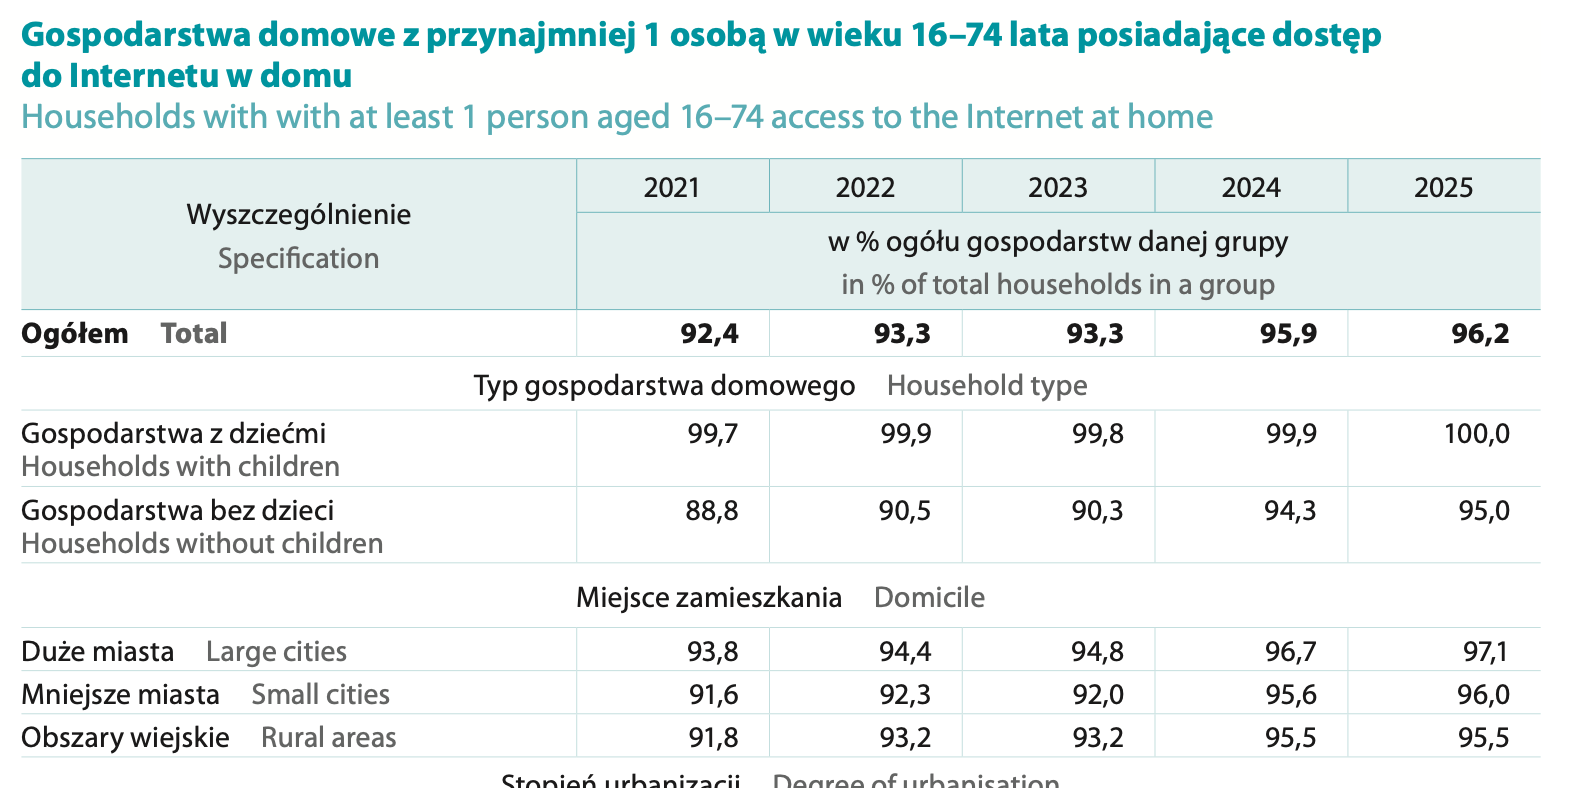
\includegraphics[width=\textwidth]{fig-1-internet/2-hh-dostep.png}
    \end{figure}
\end{frame}



\begin{frame}{Internet w Polsce -- źródło: badanie ICT GUS}
    \begin{figure}
        \centering
        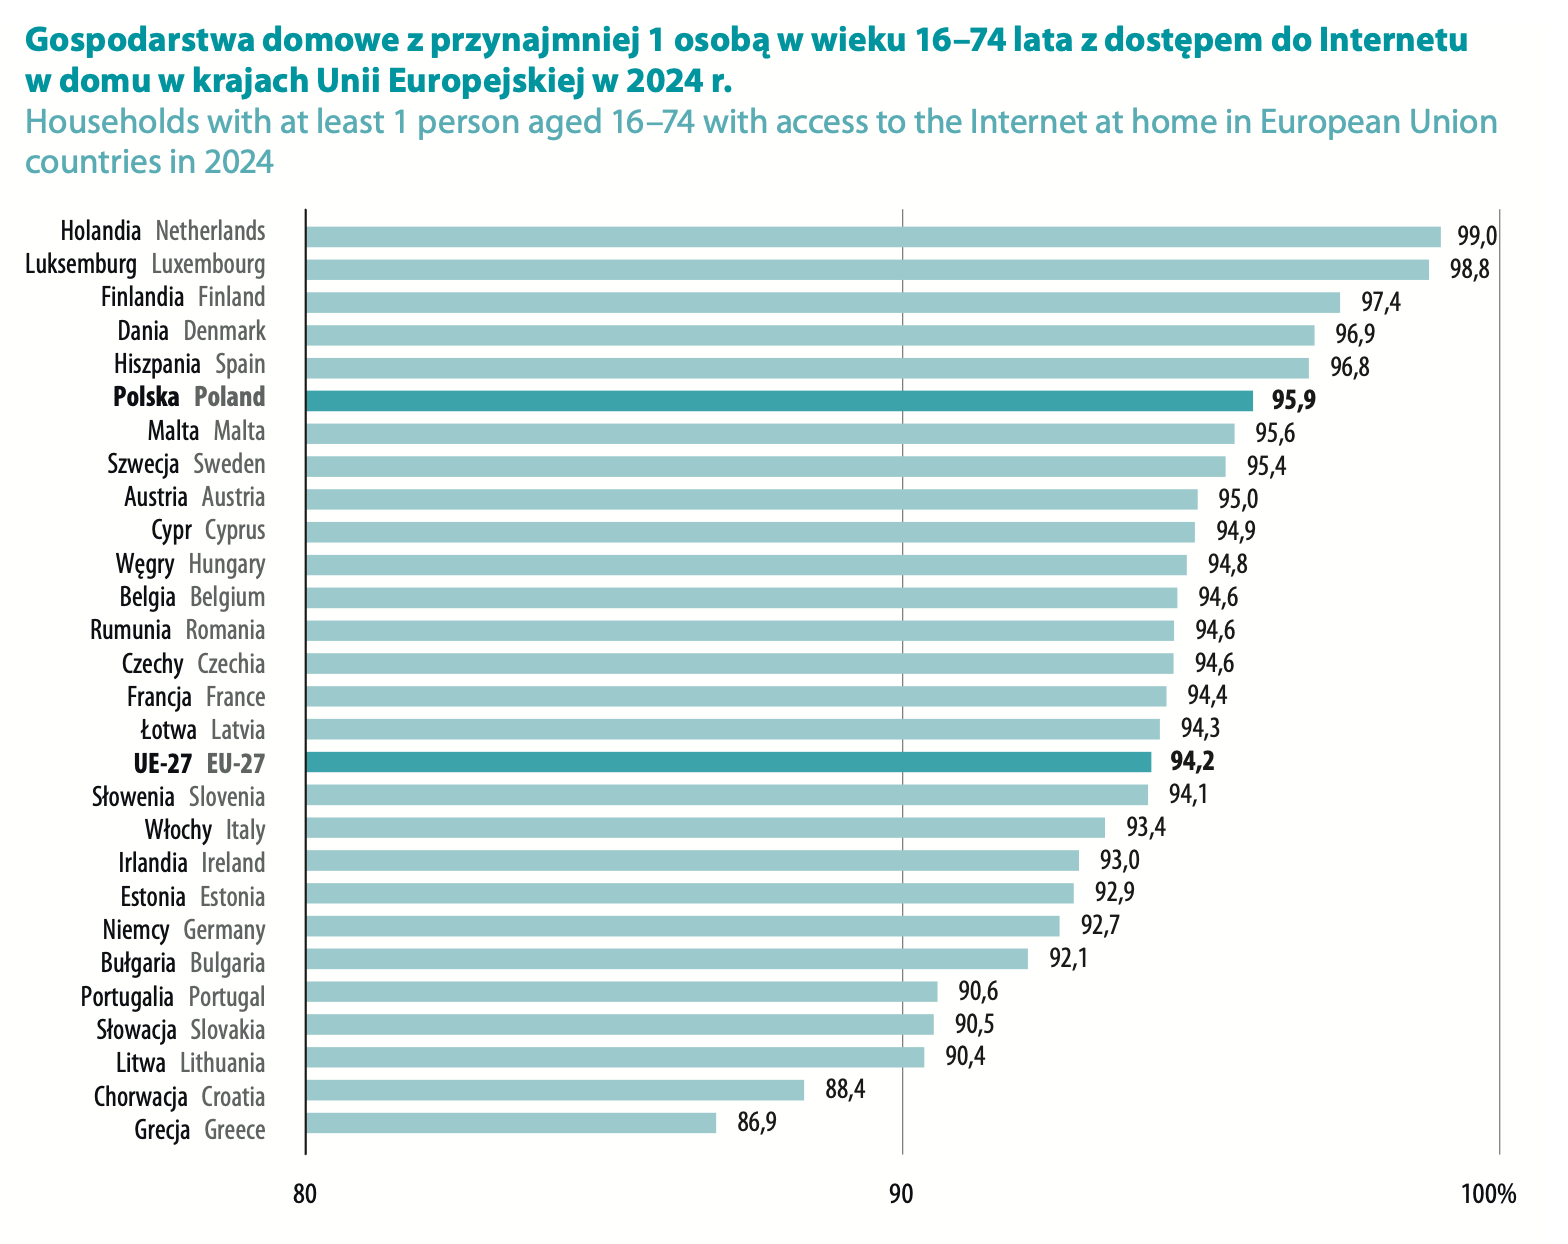
\includegraphics[width=0.6\textwidth]{fig-1-internet/3-hh-eu-dostep.png}
    \end{figure}
\end{frame}

\begin{frame}{Internet w Polsce -- źródło: badanie ICT GUS}
    \begin{figure}
        \centering
        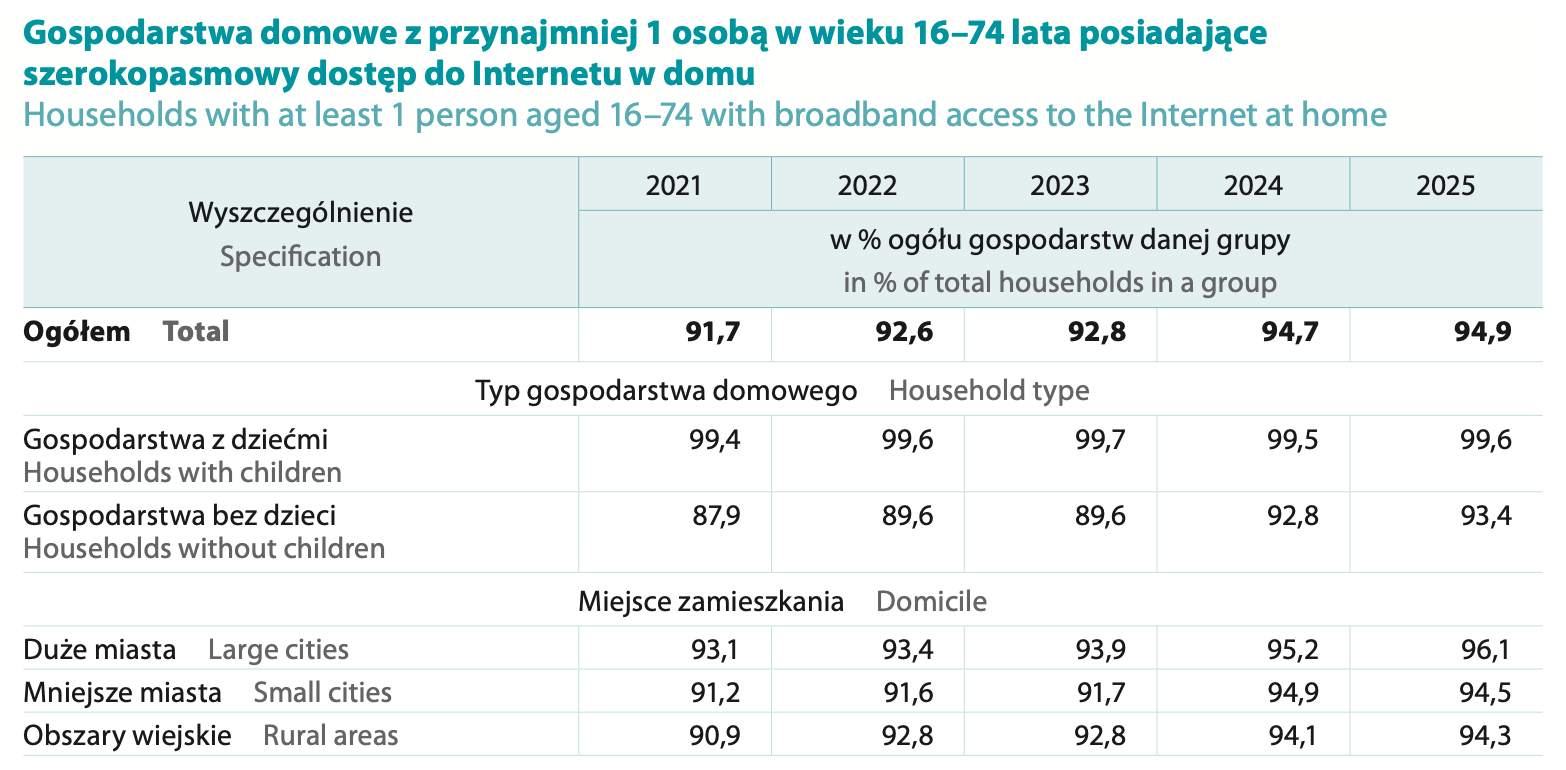
\includegraphics[width=\textwidth]{fig-1-internet/4-hh-szeroko.png}
    \end{figure}
\end{frame}

\begin{frame}{Internet w Polsce -- źródło: badanie ICT GUS}
    \begin{figure}
        \centering
        
\includegraphics[width=\textwidth]{fig-1-internet/6-os-korzyst1.png}
    \end{figure}
\end{frame}

\begin{frame}{Internet w Polsce -- źródło: badanie ICT GUS}
    \begin{figure}
        \centering
        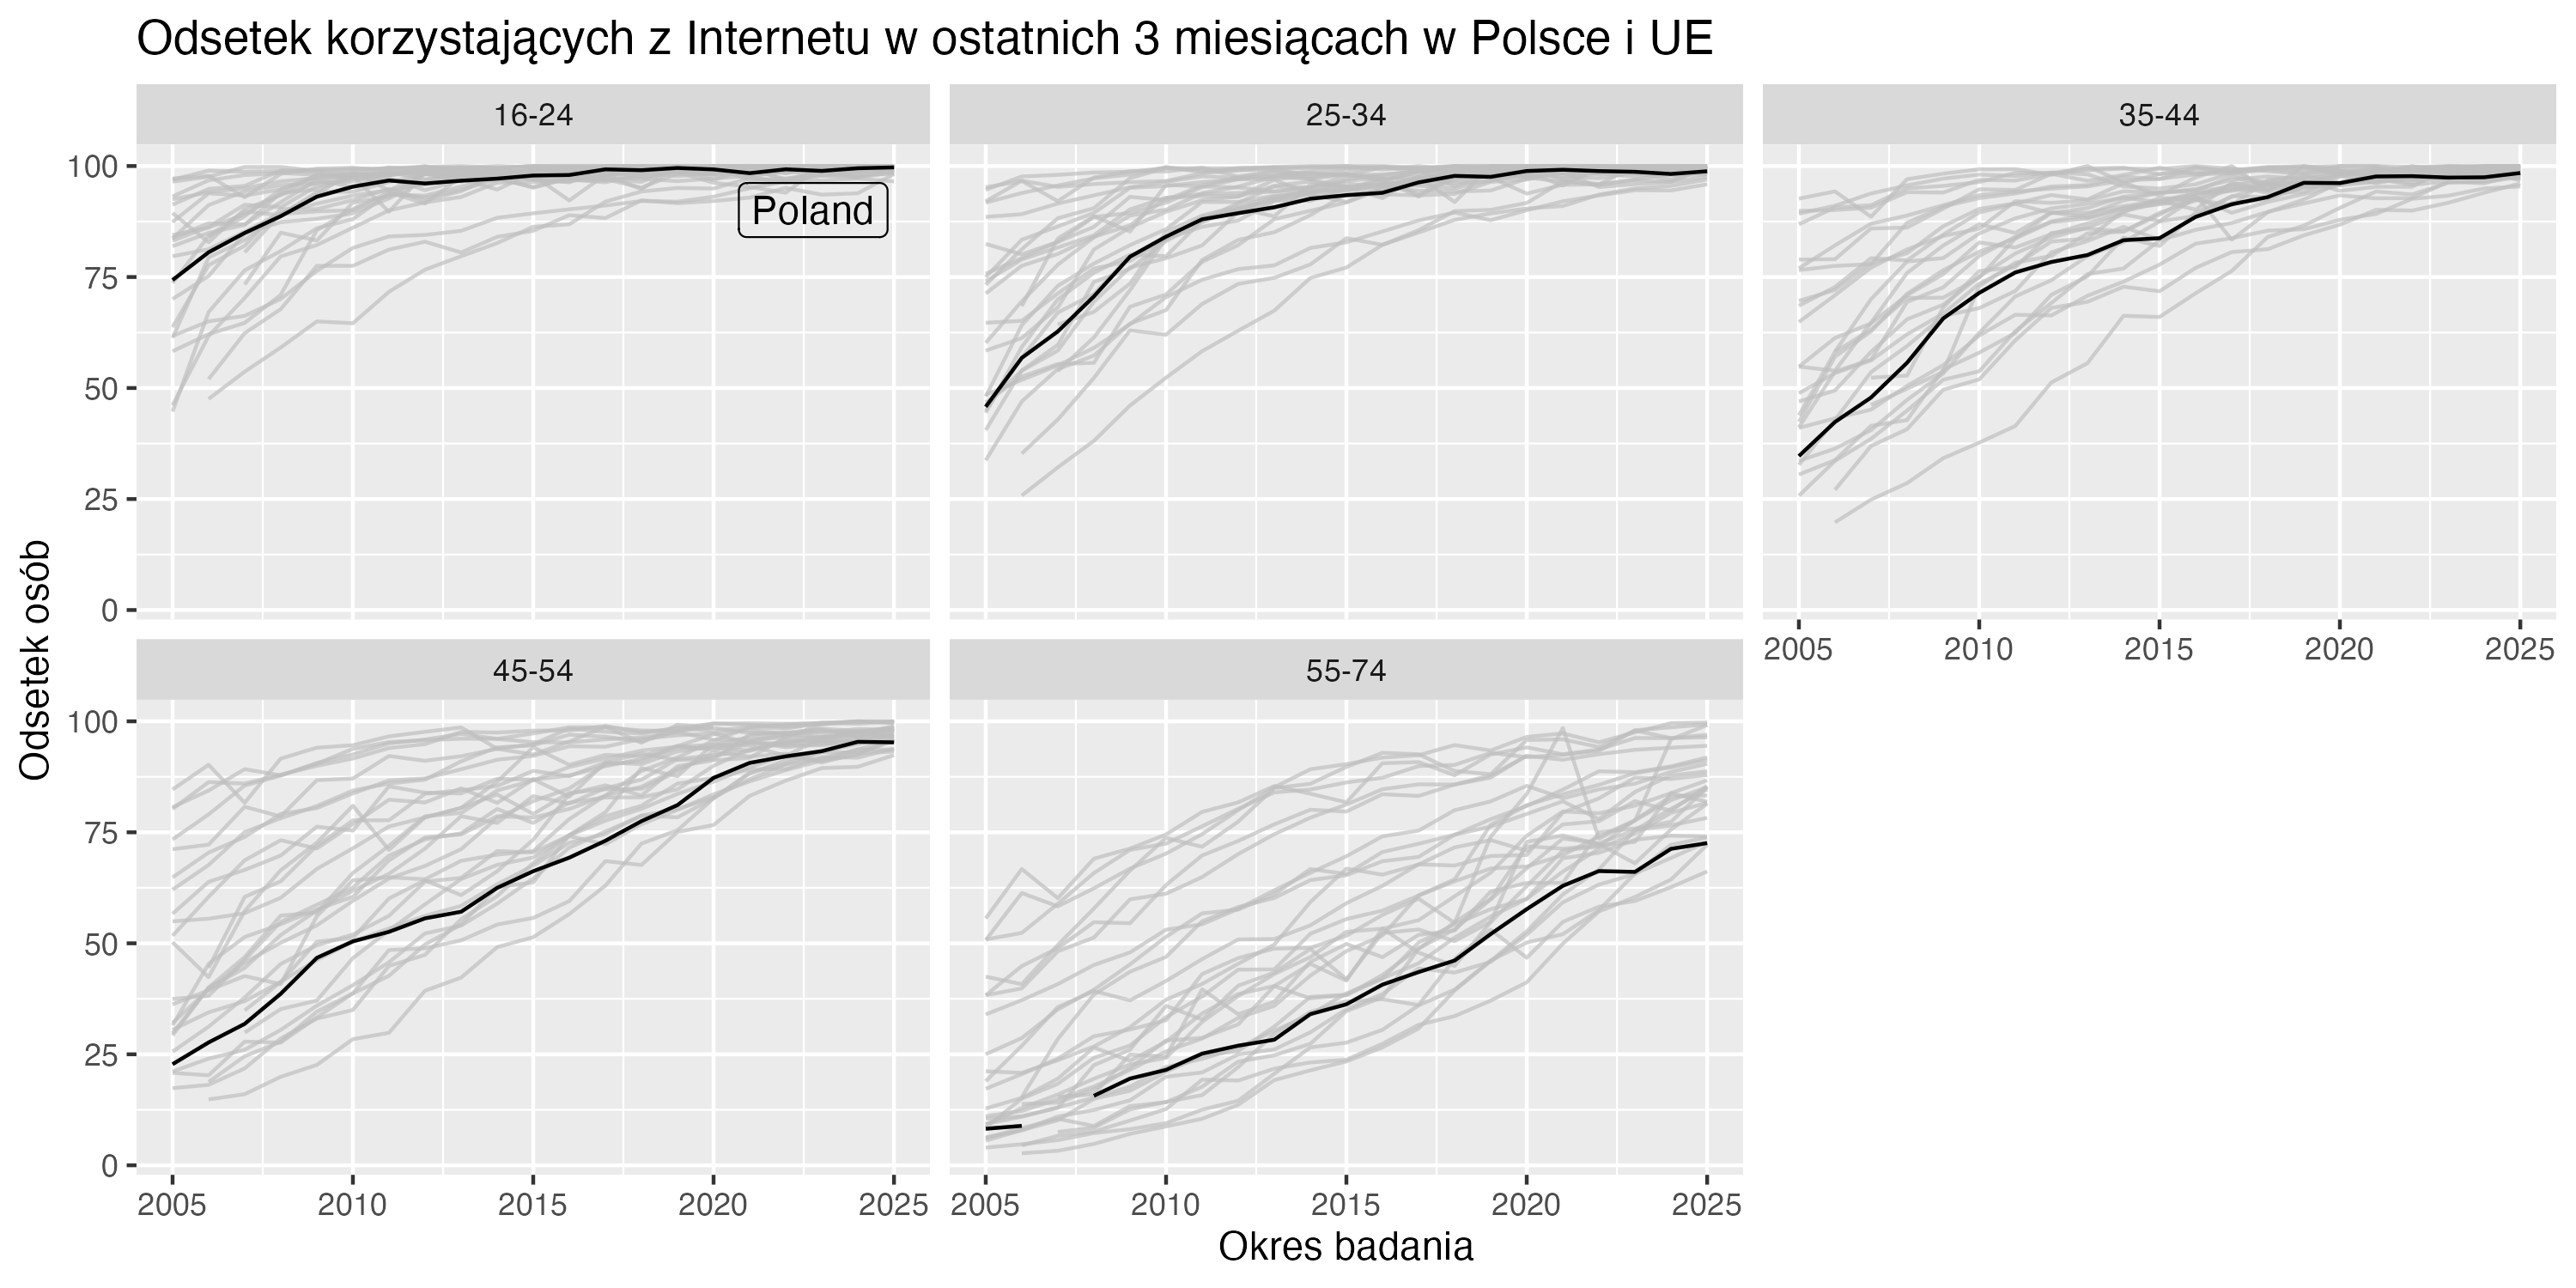
\includegraphics[width=\textwidth]{fig-1-internet/6-eurostat-wiek.png}
    \end{figure}
\end{frame}

\begin{frame}{Internet w Polsce -- źródło: badanie ICT GUS}
    \begin{figure}
        \centering
        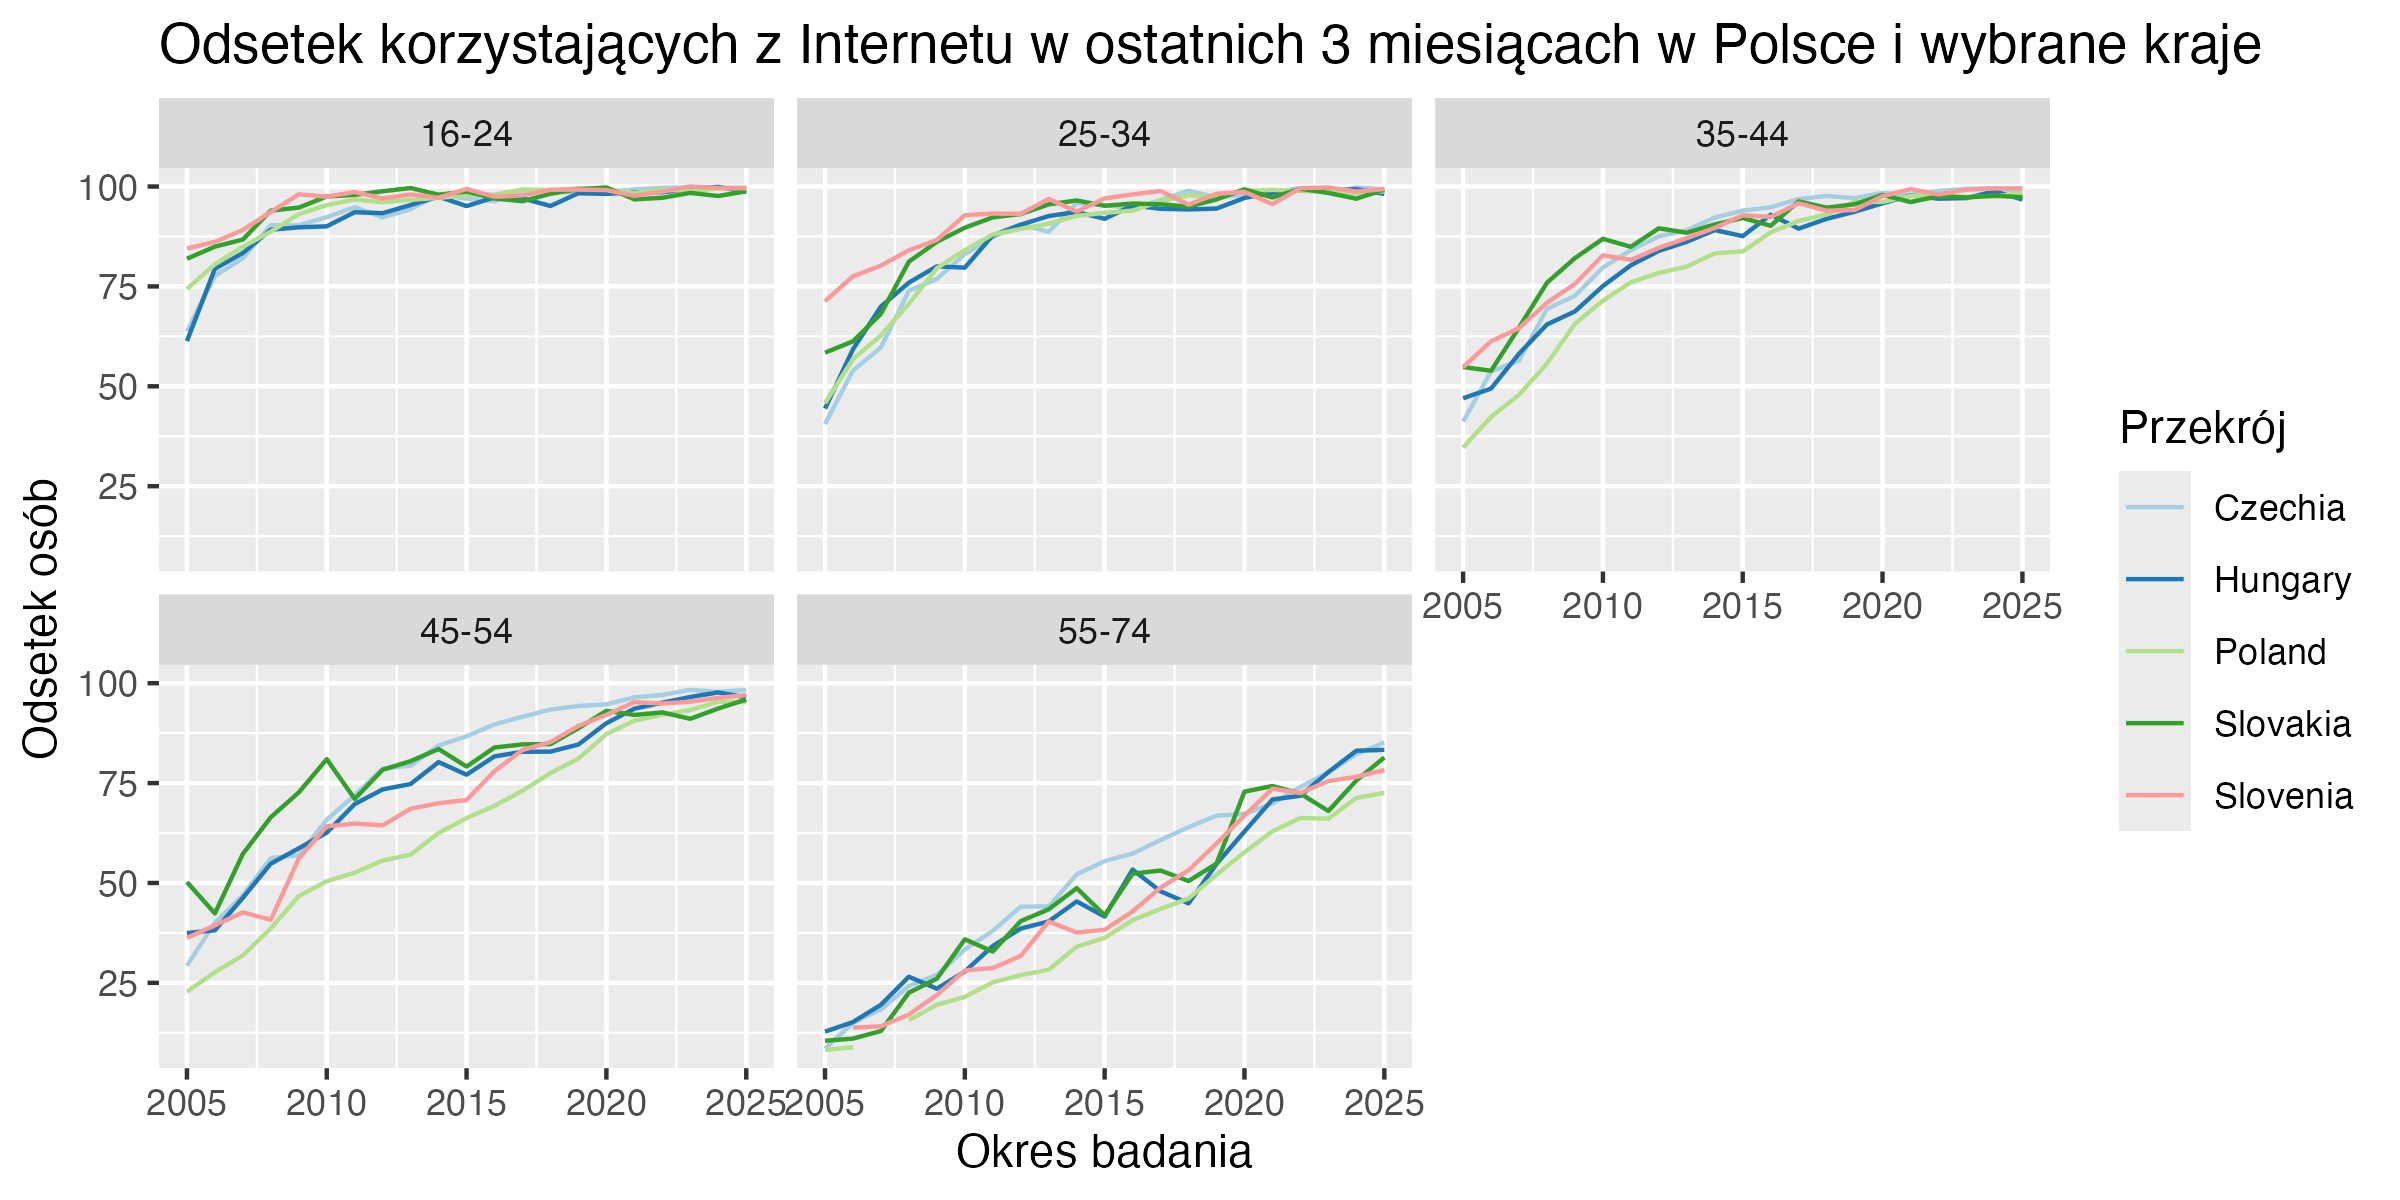
\includegraphics[width=\textwidth]{fig-1-internet/6-eurostat-sasiedzi.png}
    \end{figure}
\end{frame}

\begin{frame}{Internet w Polsce -- źródło: badanie ICT GUS}
    \begin{figure}
        \centering
        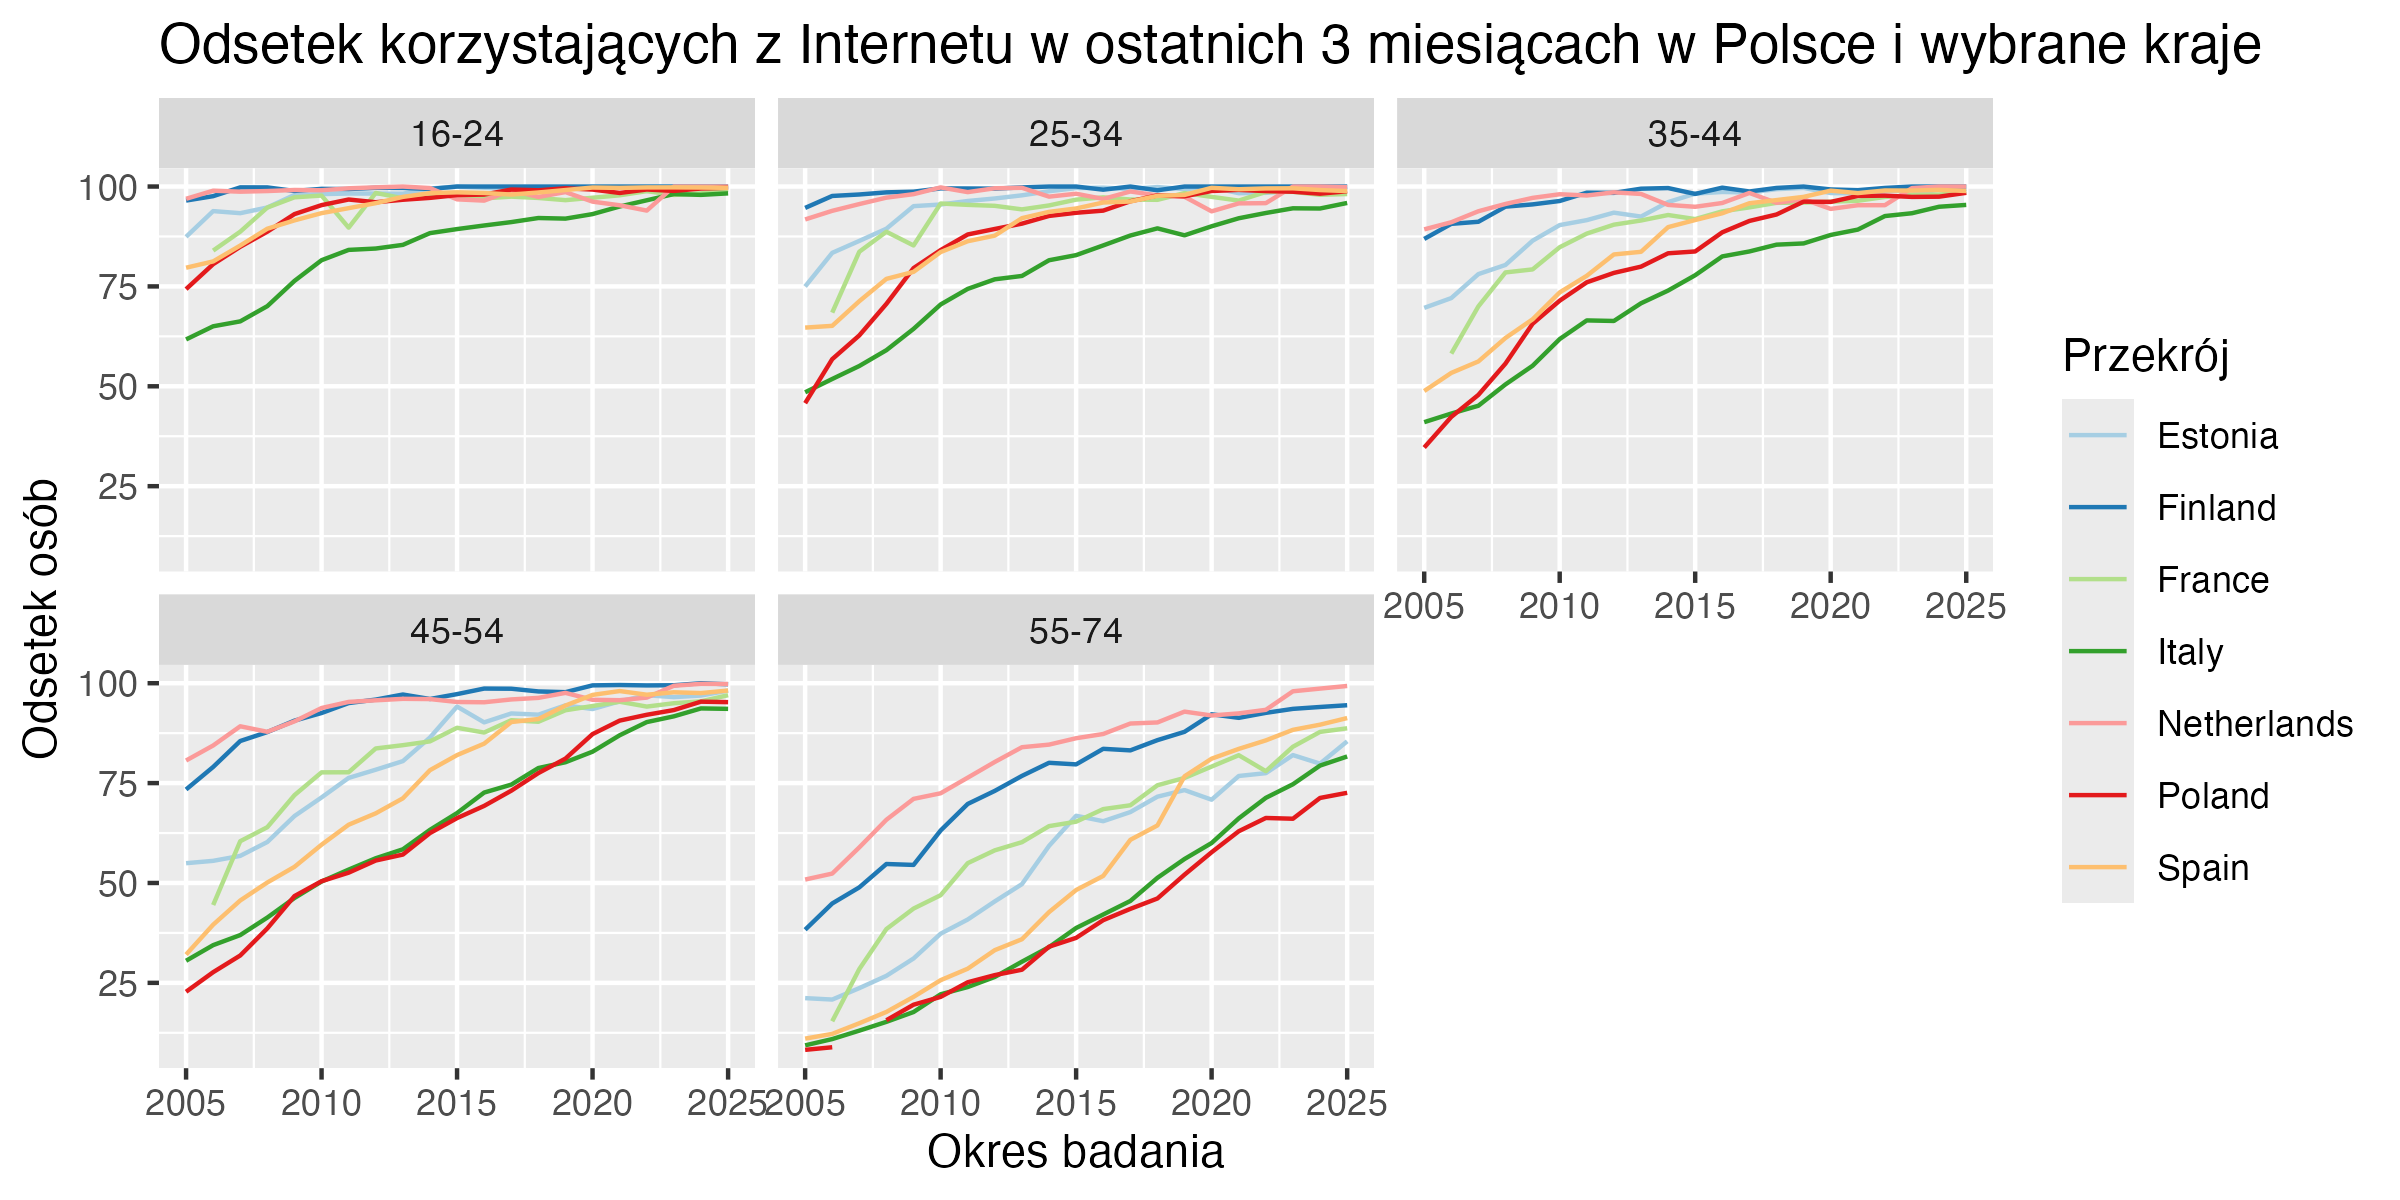
\includegraphics[width=\textwidth]{fig-1-internet/6-eurostat-inne.png}
    \end{figure}
\end{frame}


\begin{frame}{Internet w Polsce -- źródło: badanie ICT GUS}
    \begin{figure}
        \centering
        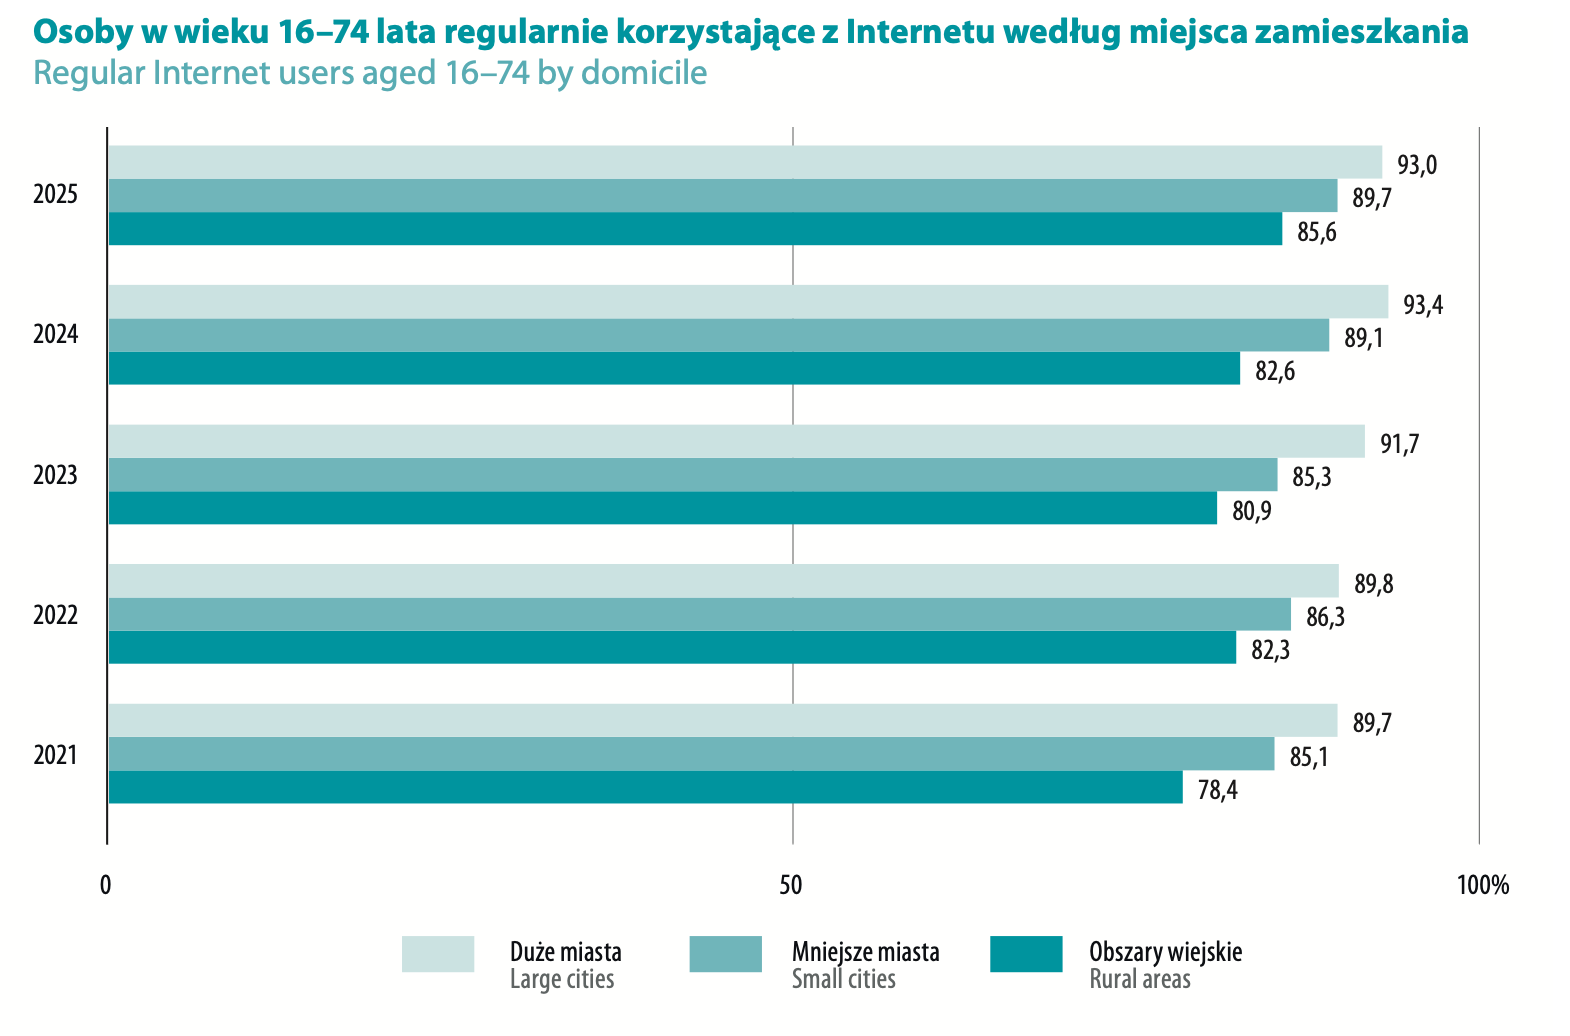
\includegraphics[width=0.8\textwidth]{fig-1-internet/6-os-regul-miejsce.png}
    \end{figure}
\end{frame}

\begin{frame}{Internet w Polsce -- źródło: badanie ICT GUS}
    \begin{figure}
        \centering
        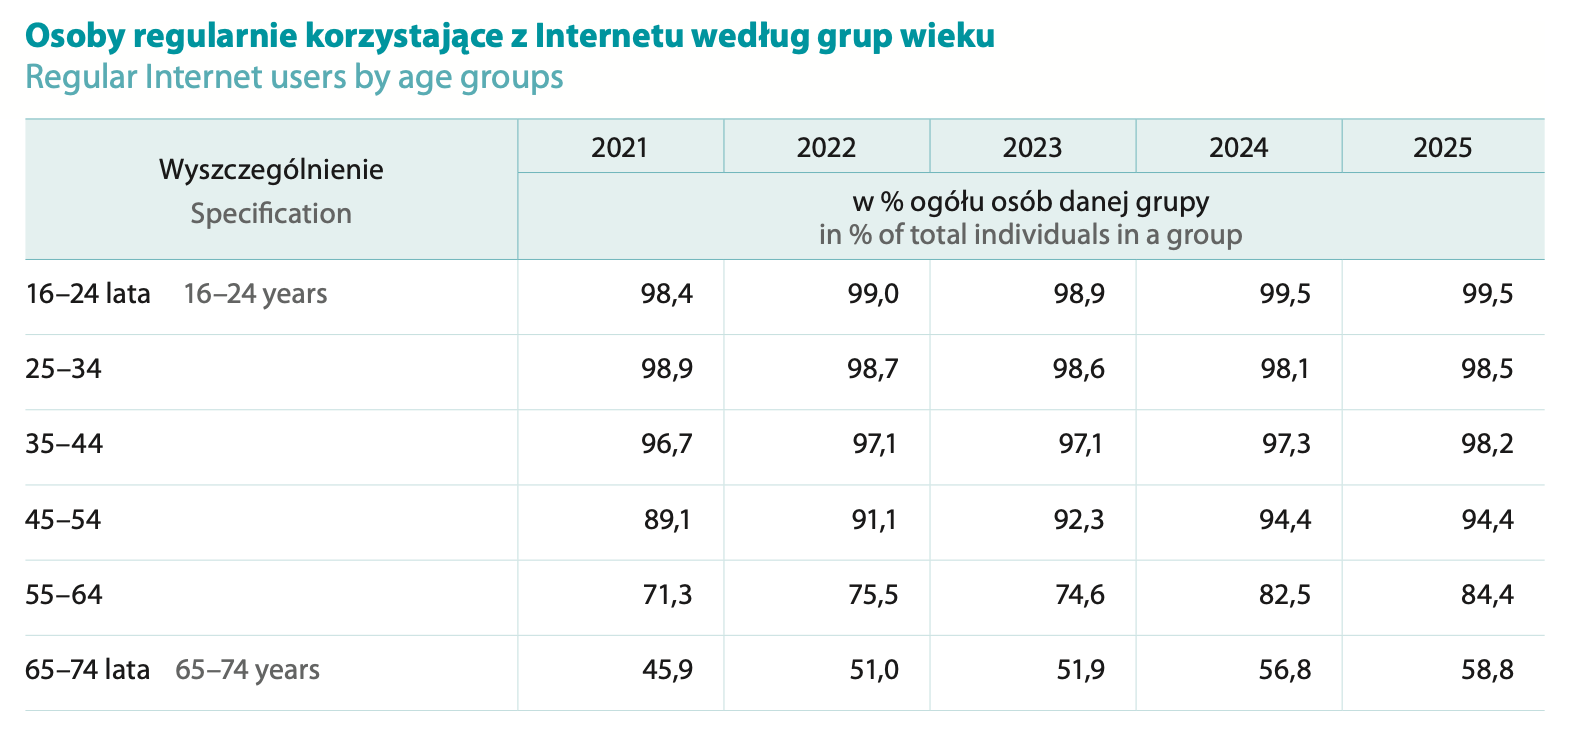
\includegraphics[width=\textwidth]{fig-1-internet/6-os-regul-wiek.png}
    \end{figure}
\end{frame}


\begin{frame}{Internet w Polsce -- źródło: badanie ICT GUS}
    \begin{figure}
        \centering
        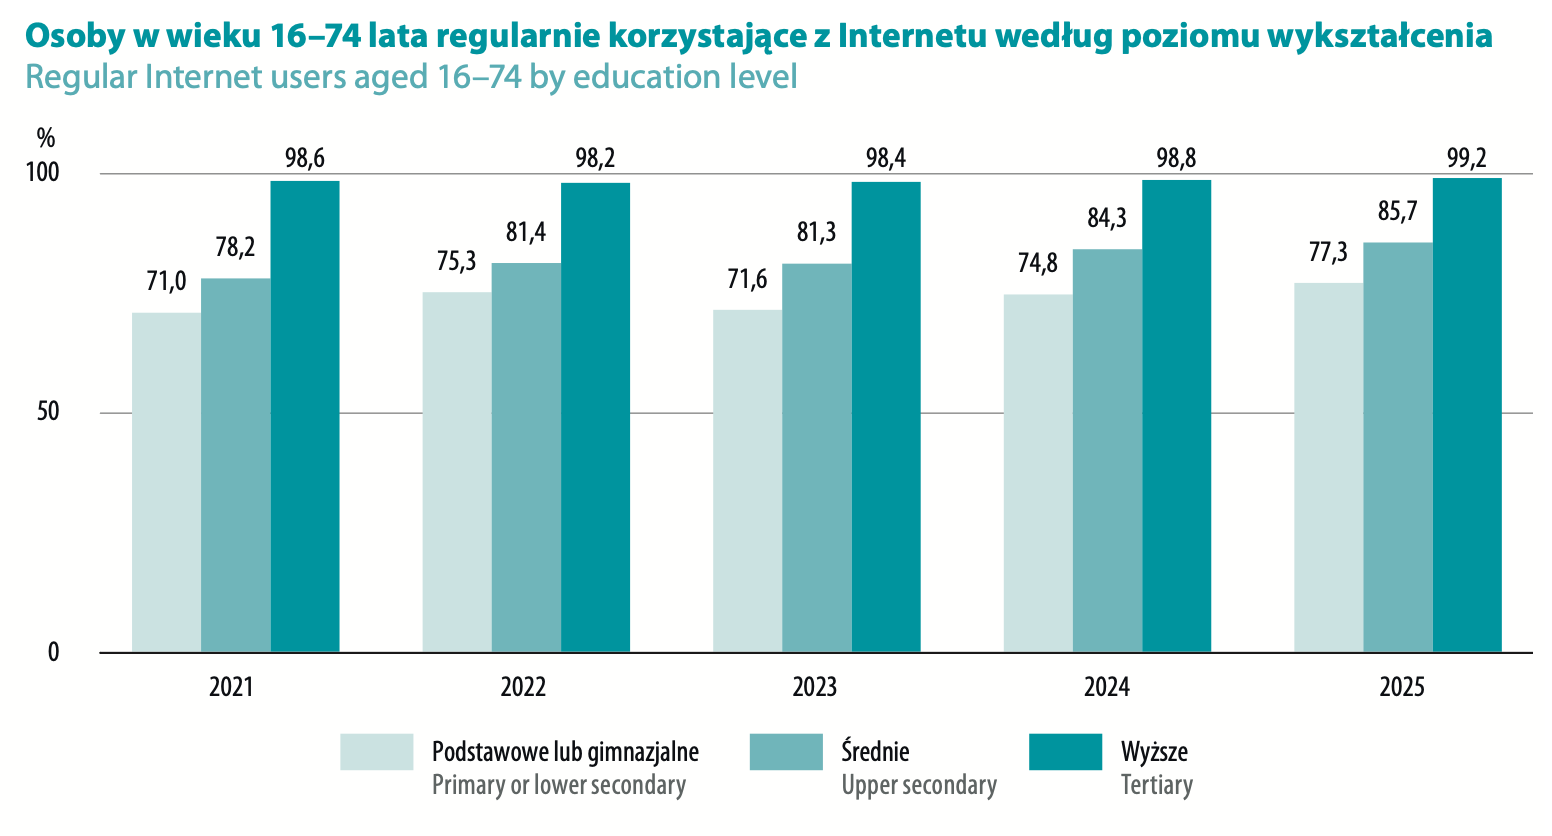
\includegraphics[width=0.9\textwidth]{fig-1-internet/6-os-regul-wyksz.png}
    \end{figure}
\end{frame}

\begin{frame}{Internet w Polsce -- źródło: badanie ICT GUS}
    \begin{figure}
        \centering
        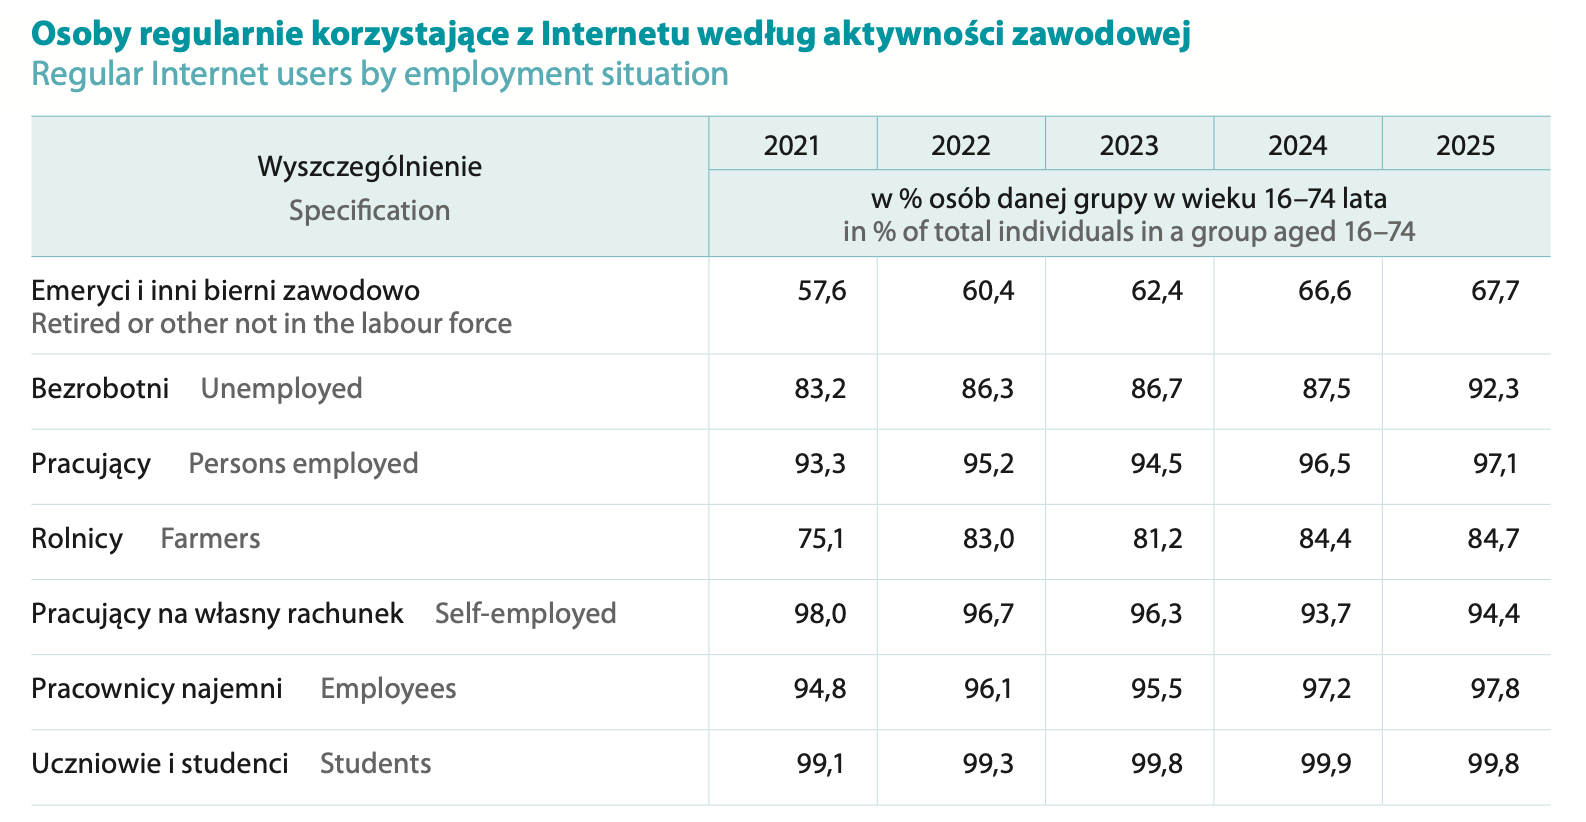
\includegraphics[width=0.9\textwidth]{fig-1-internet/6-os-regul-zawody.png}
    \end{figure}
\end{frame}


\begin{frame}{Internet w Polsce -- źródło: badanie ICT GUS}
    \begin{figure}
        \centering
        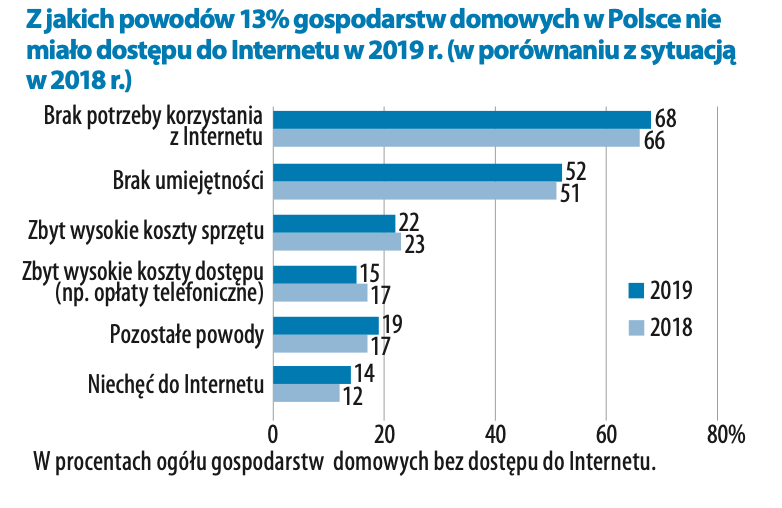
\includegraphics[width=0.8\textwidth]{fig-1-internet/9-brak-dlaczego.png}
    \end{figure}
\end{frame}

\begin{frame}{Internet w Polsce -- źródło: Diagnoza Społeczna 2015}
    \begin{figure}
        \centering
        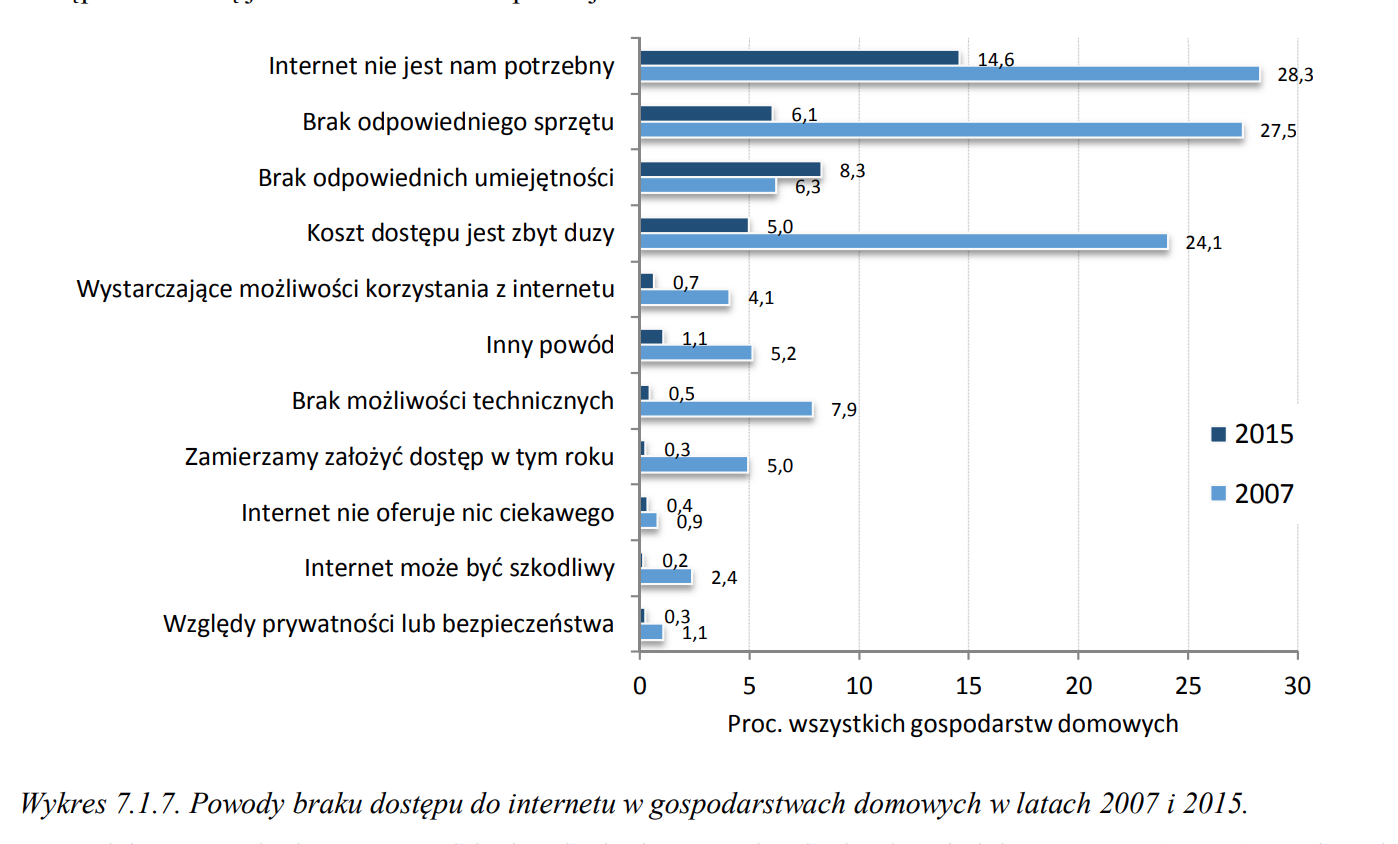
\includegraphics[width=\textwidth]{fig-1-internet/9-brak-diagnoza.png}
    \end{figure}
\end{frame}

\begin{frame}{Internet w Polsce -- źródło: BBGD 2025}
    \begin{figure}
        \centering
        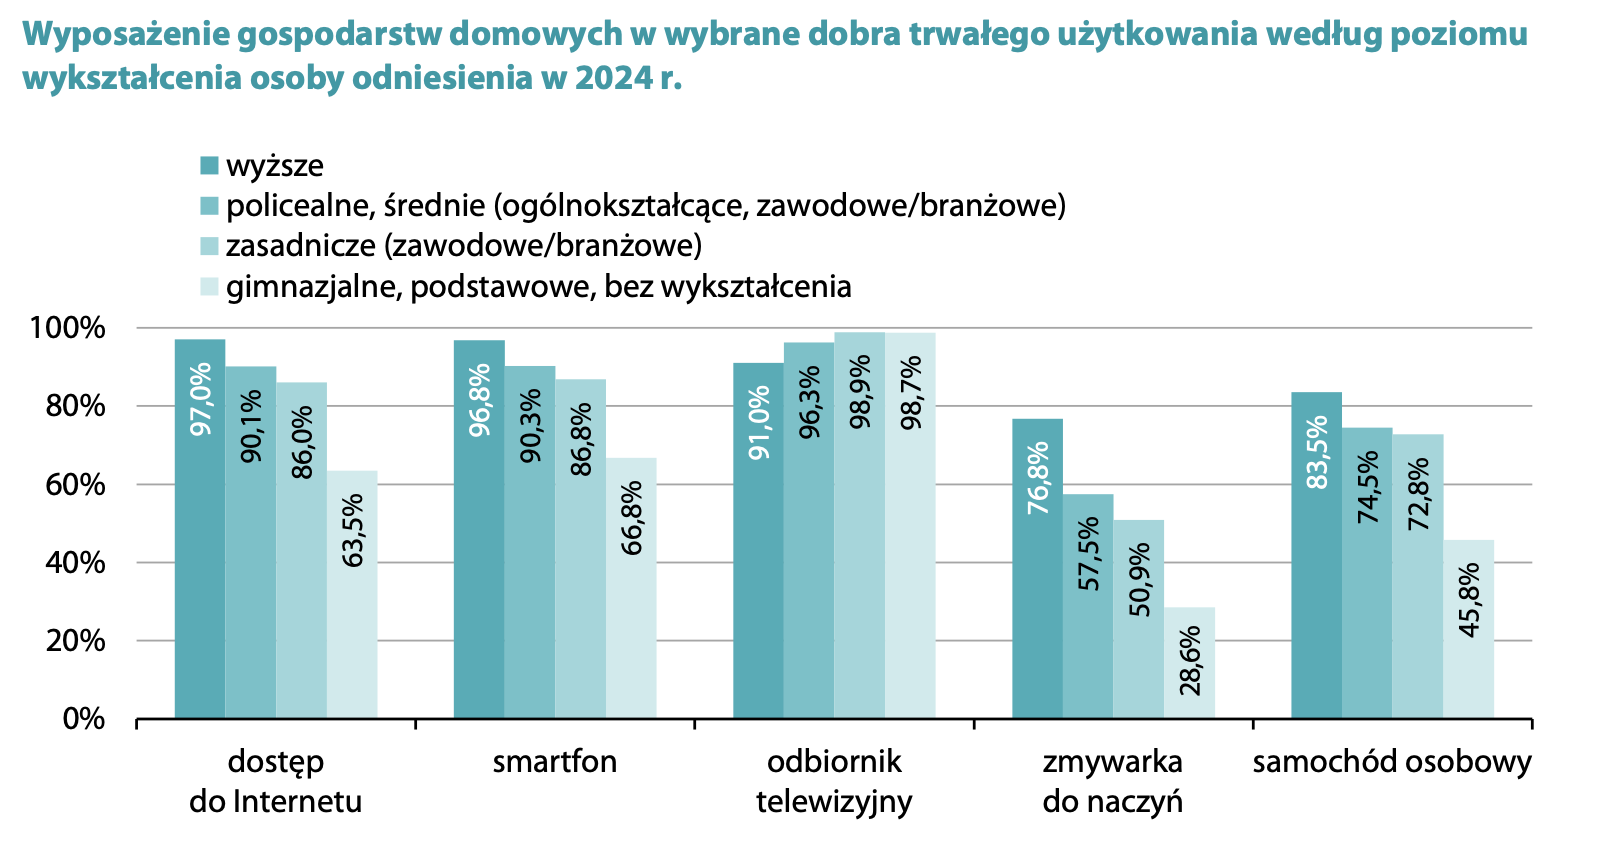
\includegraphics[width=0.9\textwidth]{fig-1-internet/10-dobra2.png}
    \end{figure}
\end{frame}

\begin{frame}{Internet w Polsce -- źródło: BBGD 2025}
    \begin{figure}
        \centering
        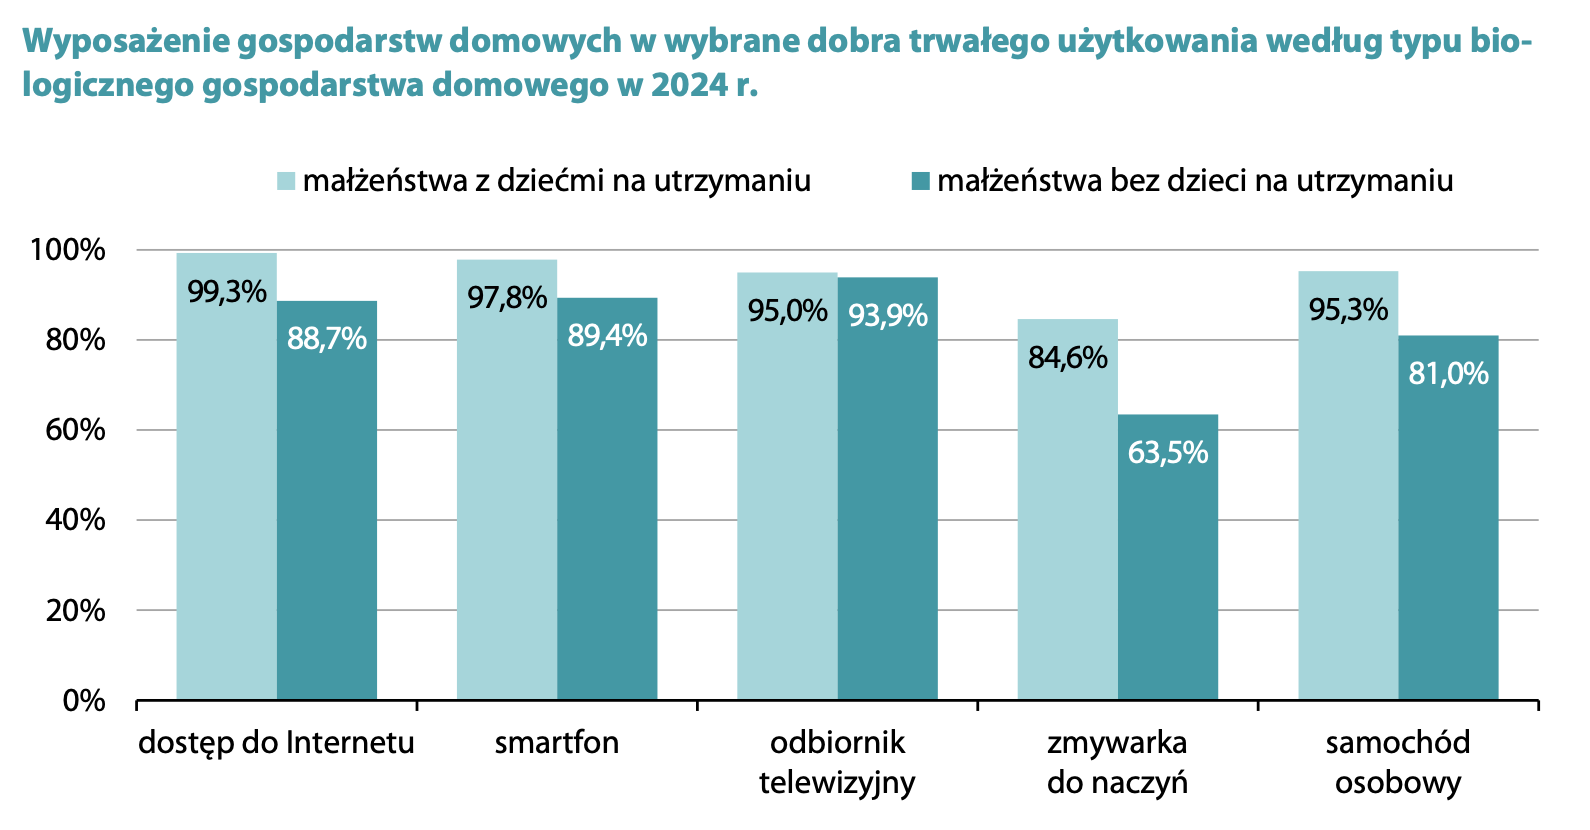
\includegraphics[width=0.9\textwidth]{fig-1-internet/10-dobra3.png}
    \end{figure}
\end{frame}

\begin{frame}{Internet w Polsce -- źródło: BBGD 2025}
    \begin{figure}
        \centering
        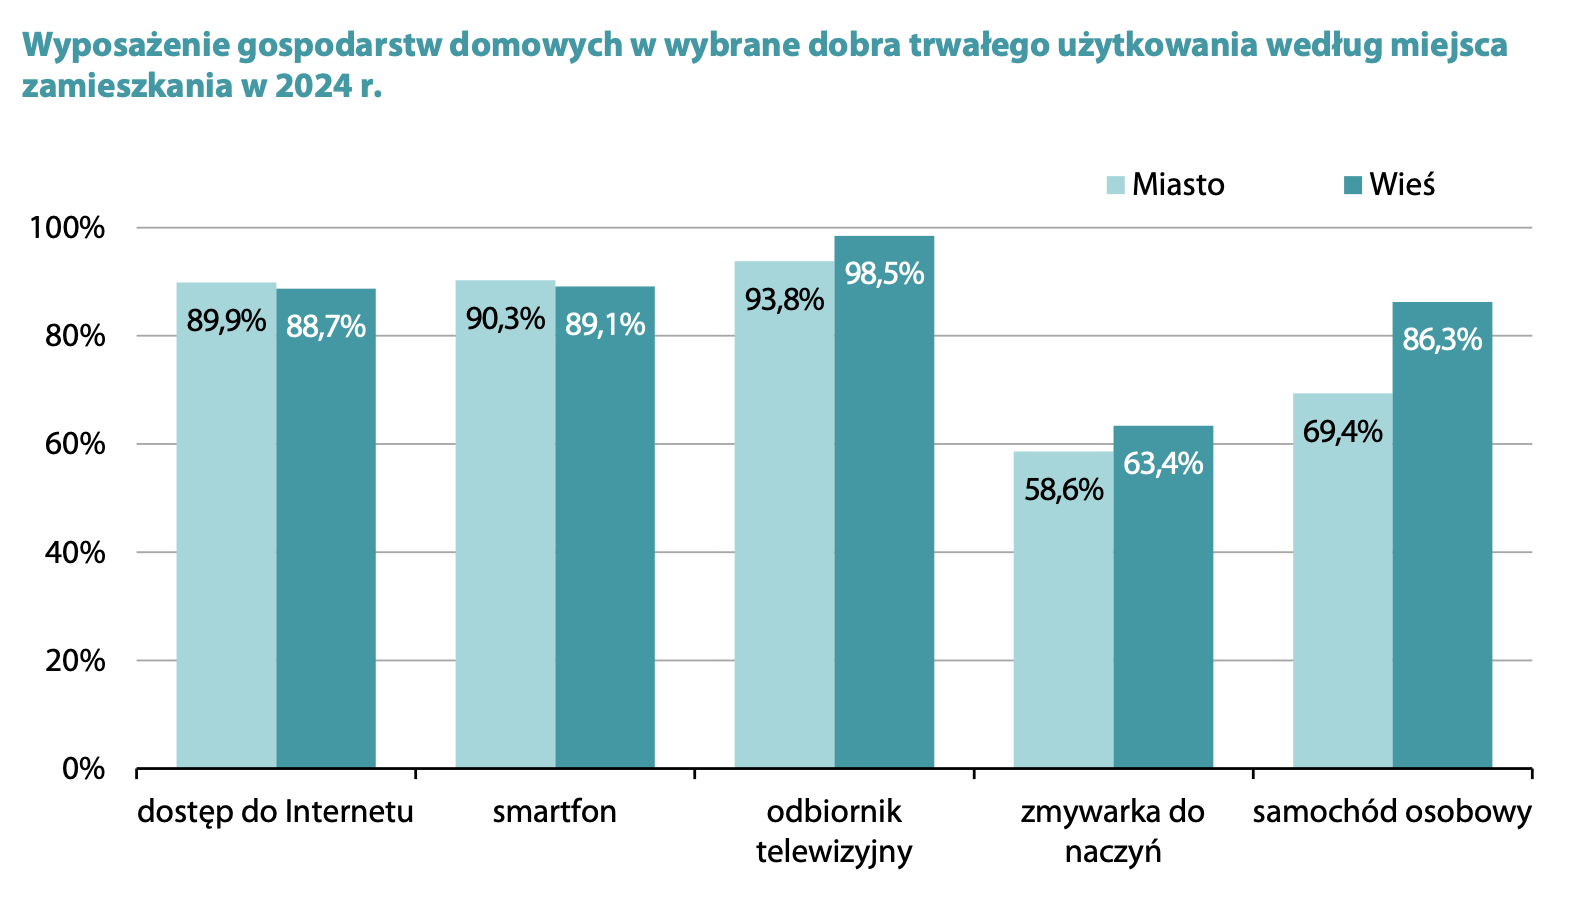
\includegraphics[width=0.9\textwidth]{fig-1-internet/10-dobra4.png}
    \end{figure}
\end{frame}

\begin{frame}{Internet w Polsce -- literatura}
    Literatura użyta na potrzeby zajęć o Internecie w Polsce
    
    \begin{itemize}
    \small
        \item GUS (2026), Społeczeństwo informacyjne w Polsce w 2025 r., \url{https://stat.gov.pl/obszary-tematyczne/nauka-i-technika-spoleczenstwo-informacyjne/spoleczenstwo-informacyjne/spoleczenstwo-informacyjne-w-polsce-w-2022-roku,1,16.html}.
        \item GUS (2025), Budżety gospodarstw domowych w 2024 roku, \url{https://stat.gov.pl/obszary-tematyczne/warunki-zycia/dochody-wydatki-i-warunki-zycia-ludnosci/budzety-gospodarstw-domowych-w-2024-r-,9,23.html}
        \item Czapiewski (2016) Raport z badania Diagnoza Społeczna 2015, \url{www.diagnoza.com}
    \end{itemize}
\end{frame}

% %%%%%%%%%%%% discrete dists %%%%%%%%%%%%%%%%%%

\section{Google Trends i inne serwisy} 

\begin{frame}{Google Trends}
    \begin{figure}
        \centering
        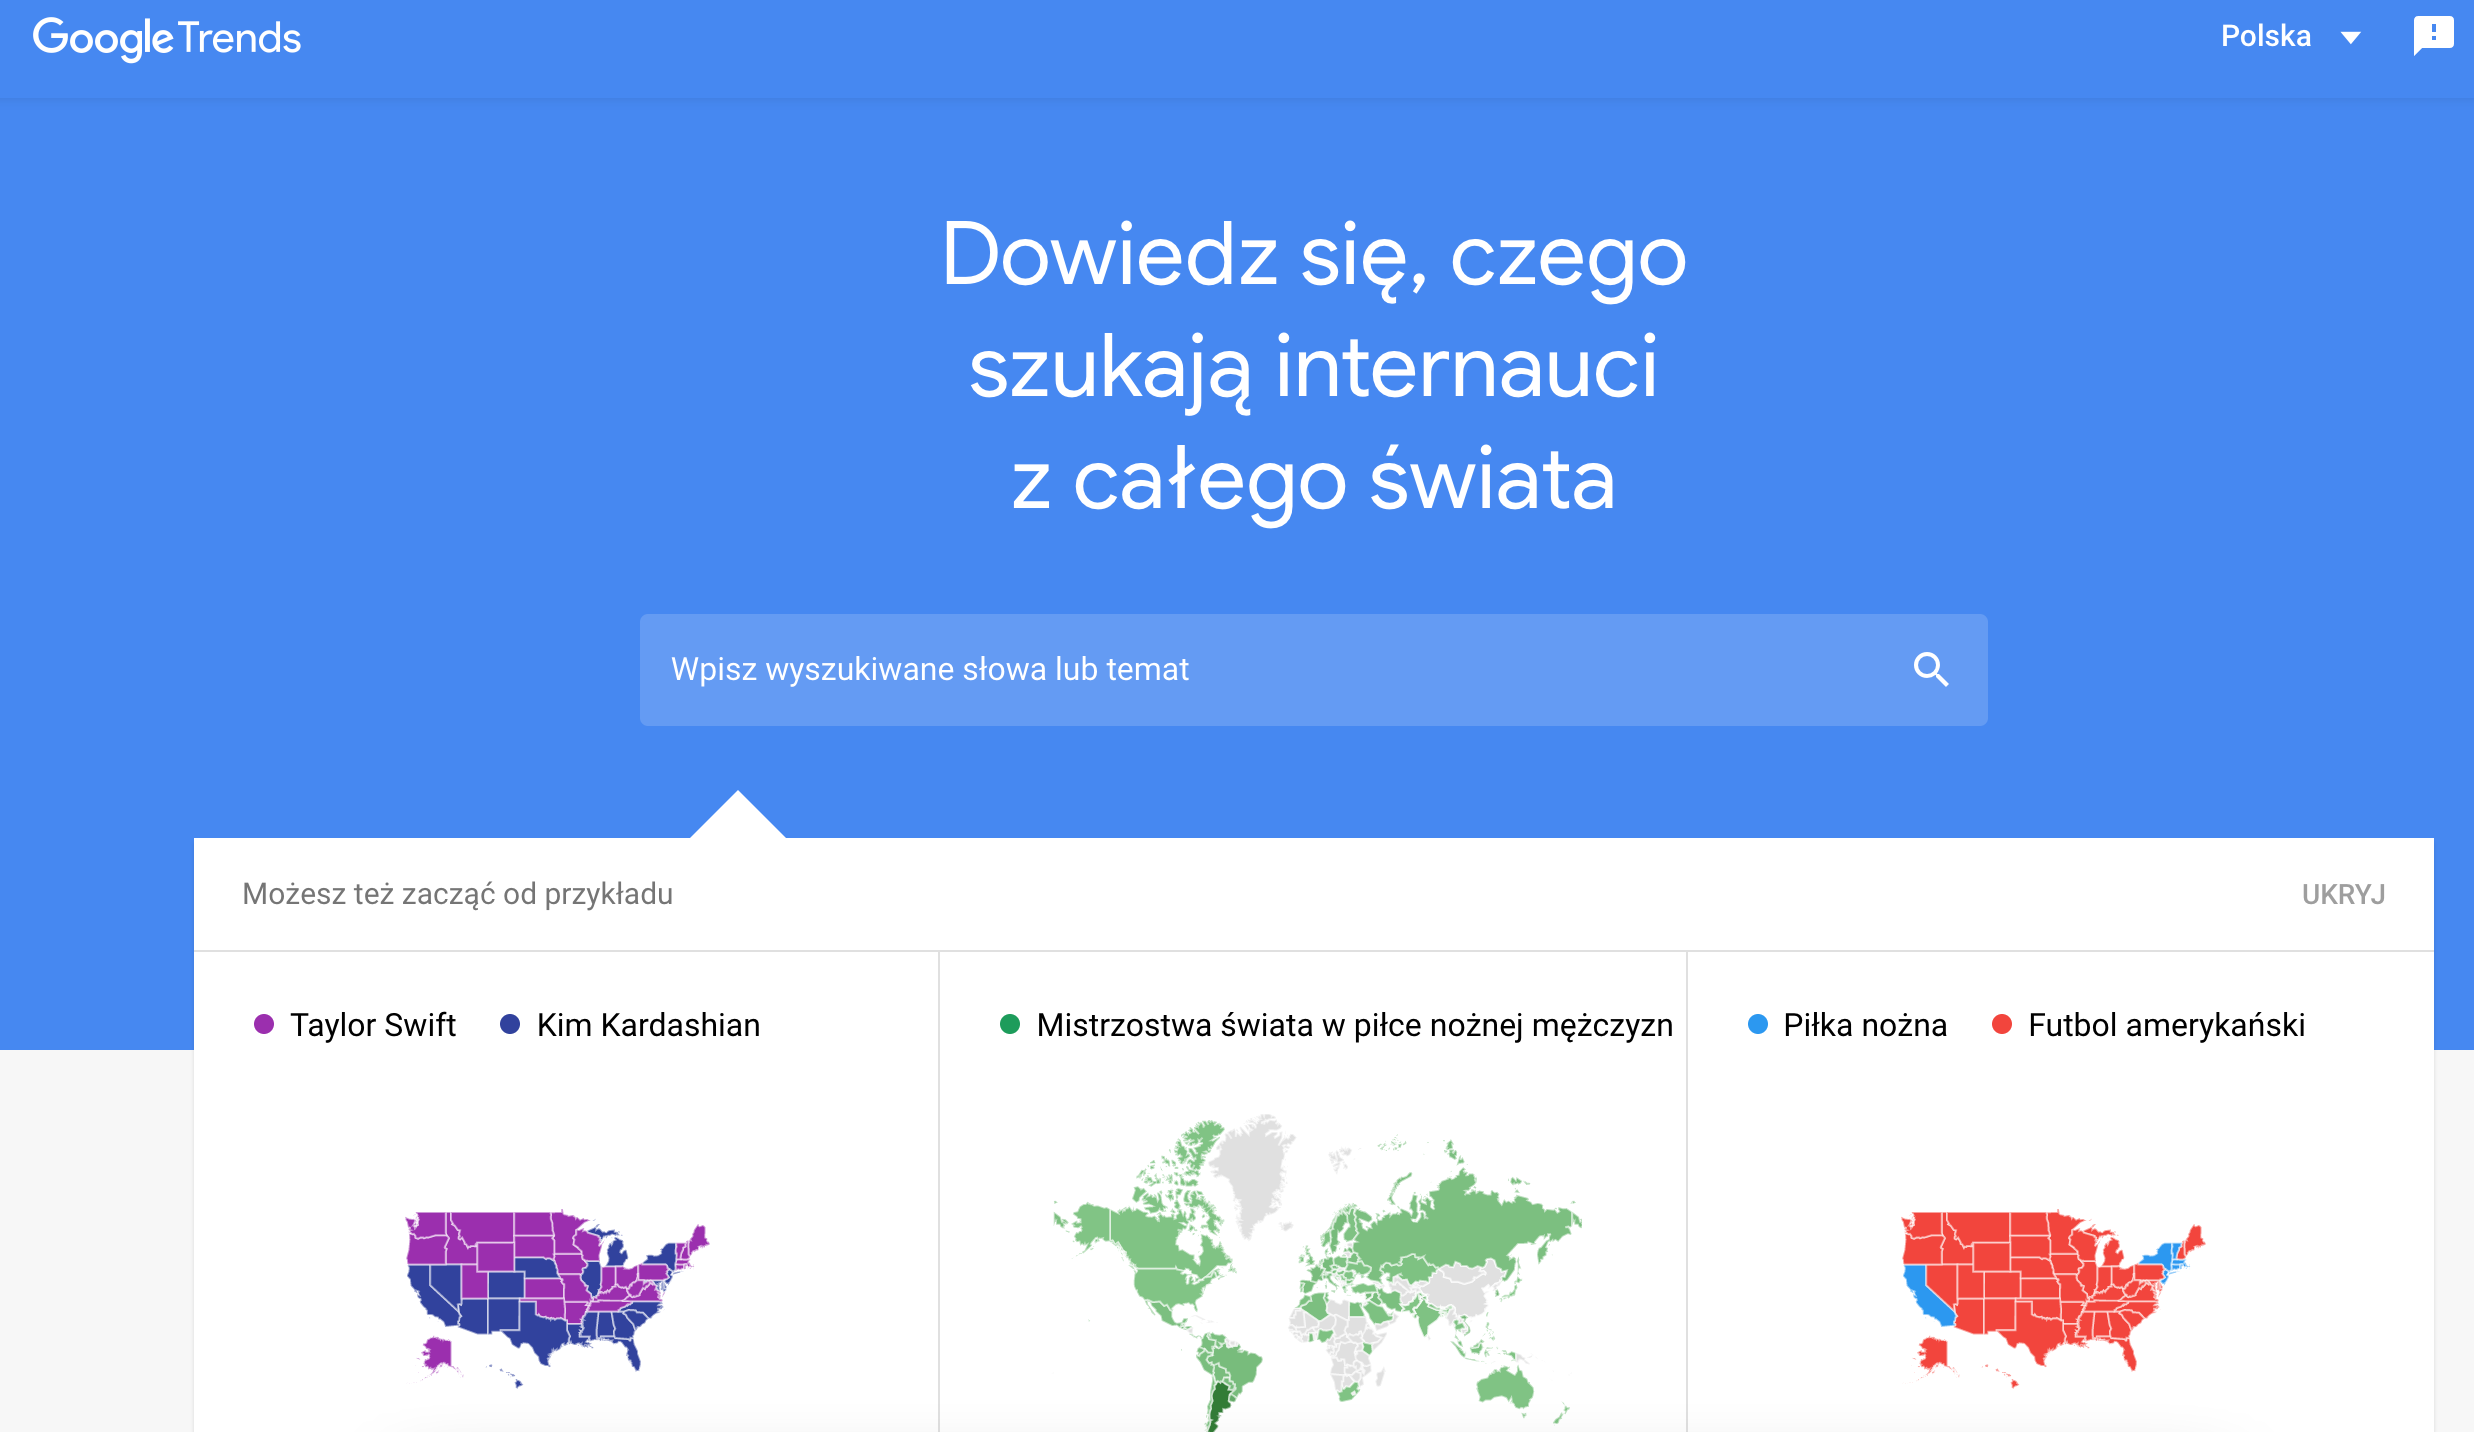
\includegraphics[width=\textwidth]{fig-7-trends/gtrends.png}
        \caption{Strona główna Google Trends}
    \end{figure}
\end{frame}

\begin{frame}{Google Trends -- podstawowe informacje}
    \begin{itemize}
        \item 11 maj 2006 -- start jako "Google Insights for Search".
        \item 27 września 2012 -- powstanie Google Trends w formie, którą teraz znamy.
        \item Trendy Google zapewniają dostęp do zasadniczo niefiltrowanej próbki rzeczywistych żądań wyszukiwania wysyłanych do Google.
        \item Dane te są zanonimizowane (nie można rozpoznać użytkowników), podzielone na kategorie (z określonym tematem wyszukiwanych haseł) i zagregowane (pogrupowane).
        \item W Trendach Google dostępne są dwa rodzaje próbek danych:
        \begin{itemize}
            \item Dane w czasie rzeczywistym to próbka obejmująca ostatnie siedem dni.
            \item Dane niedynamiczne stanowią osobną próbkę i obejmują okres od 2004 roku do 36 godzin przed wyszukiwaniem.
        \end{itemize}
        \item Dane Google Trends podlegają normalizacji.
    \end{itemize}
\end{frame}

\begin{frame}{Google Trends -- normalizacja}
    \begin{figure}
        \centering
        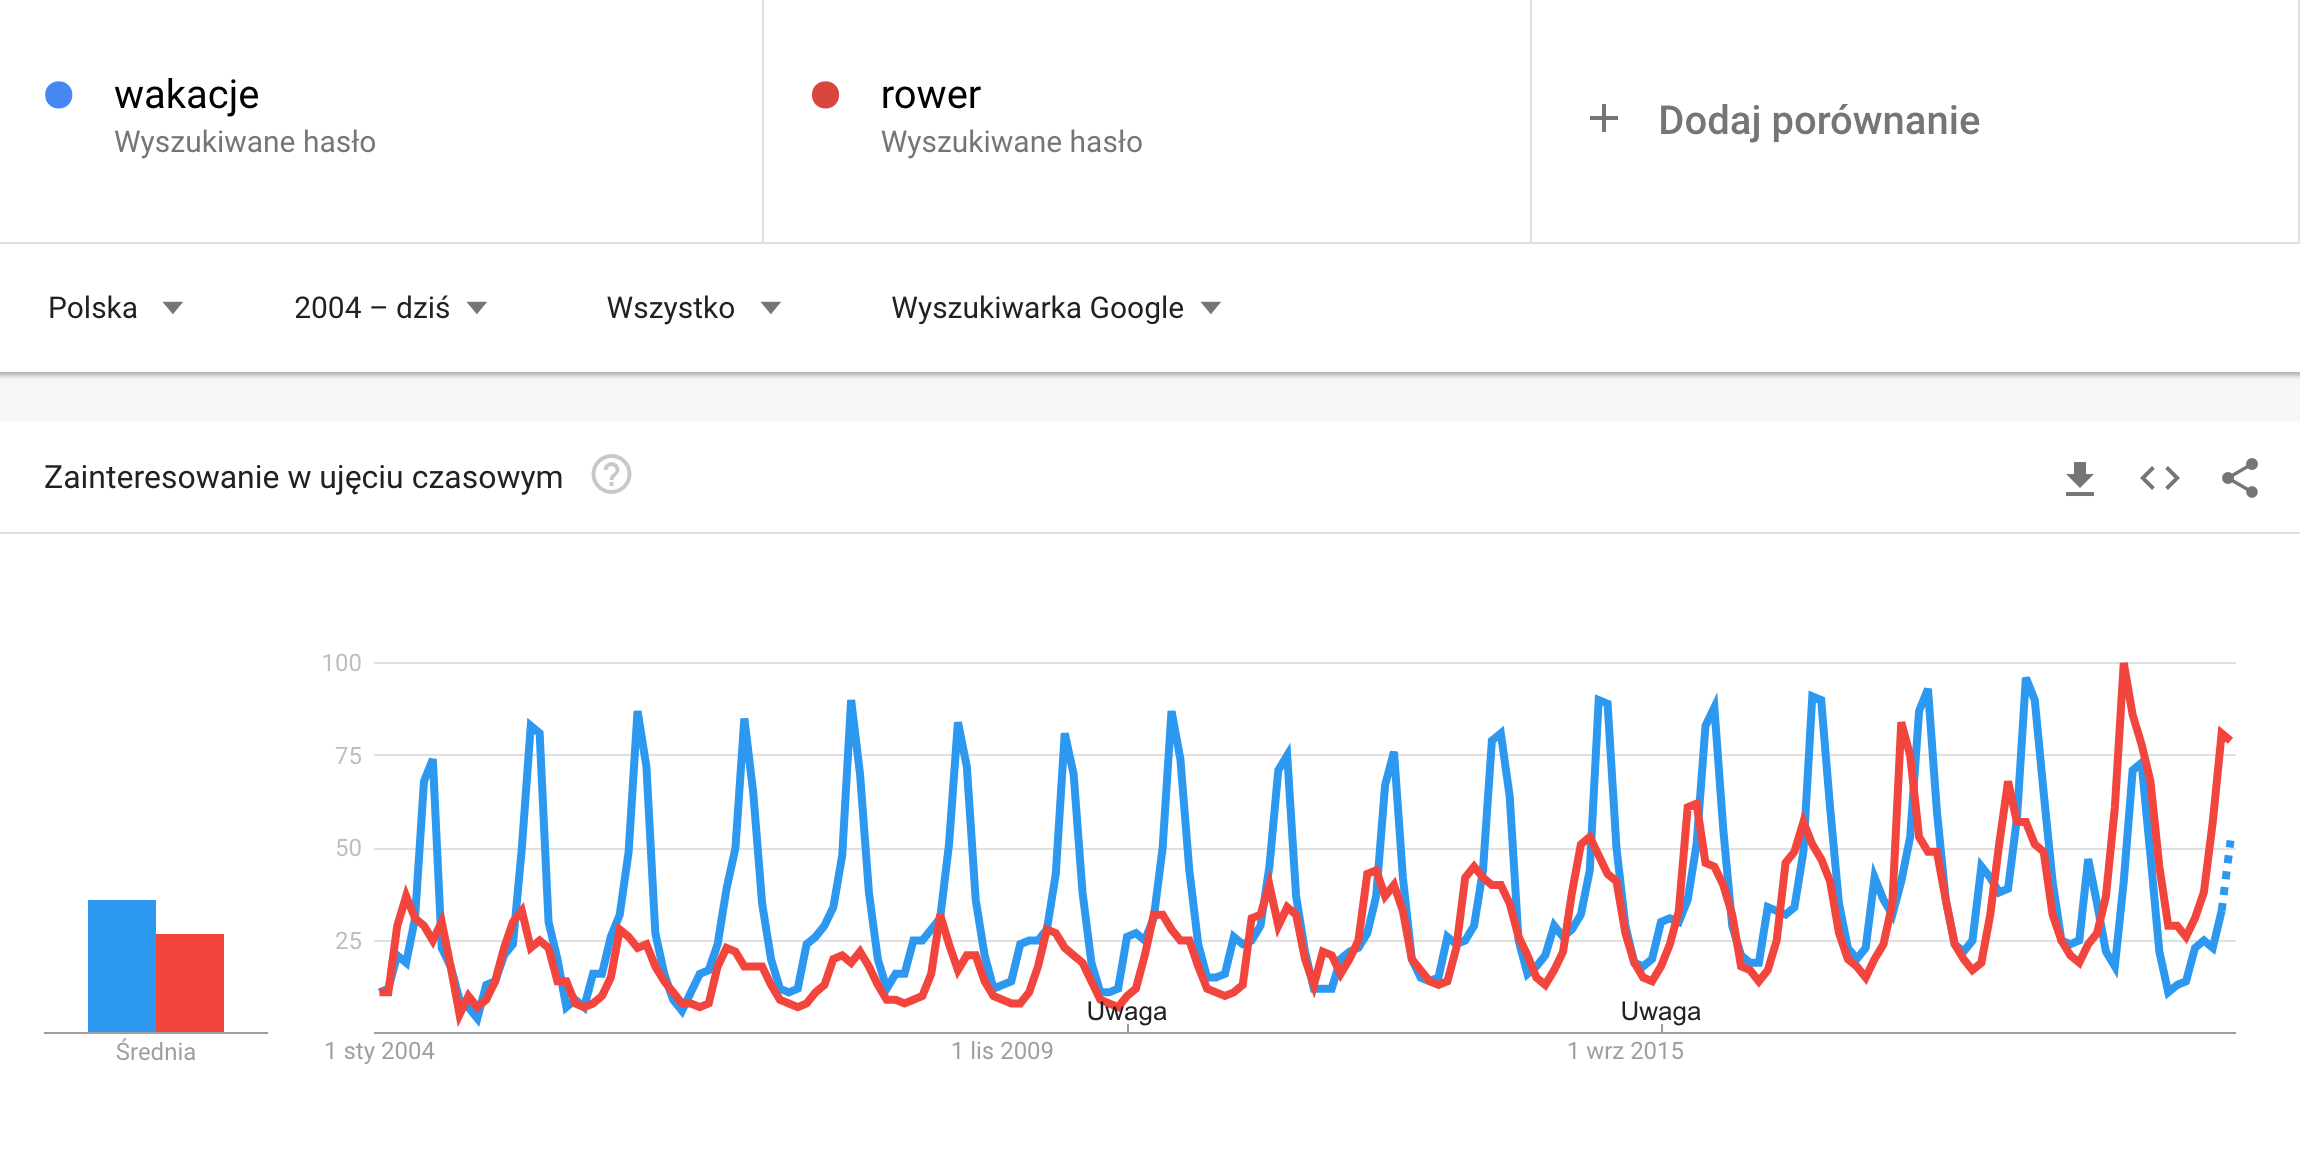
\includegraphics[width=\textwidth]{fig-7-trends/gtrends-norm.png}
        \caption{Przykład zapytania i normalizacji}
    \end{figure}
\end{frame}

\begin{frame}{Google Trends -- normalizacja}
Trendy Google normalizują dane wyszukiwania, by ułatwić porównywanie haseł. Wyniki wyszukiwania są normalizowane względem czasu i lokalizacji wyszukiwania w ten sposób:
    \begin{itemize}
    \justifying    
        \item Każdy punkt danych jest dzielony przez łączną liczbę wyszukiwań w danym regonie i okresie, co pozwala ocenić jego względną popularność. W przeciwnym razie regiony, w których wyszukiwań jest najwięcej, zawsze byłyby najwyżej w rankingu.
\item Rezultat jest następnie skalowany w zakresie od 0 do 100 na podstawie proporcjonalności tematu względem wszystkich wyszukiwań wszystkich tematów.
\item Jeśli w różnych regionach zainteresowanie wyszukiwaniem wybranego hasła jest takie samo, nie oznacza to jeszcze, że łączna liczba wyszukiwań jest w nich również taka sama.
    \end{itemize}
\end{frame}

\begin{frame}{Google Trends -- jakość danych}
    \begin{itemize}
    \justifying
        \item Dane w Trendach Google odzwierciedlają codzienne wyszukiwania w Google. 
        \item Mogą też pokazywać nieprawidłową aktywność związaną z wyszukiwaniem, np. wyszukiwanie zautomatyzowane lub zapytania potencjalnie związane z próbami spamowania wyników wyszukiwania.
        \item Trendy Google odfiltrowują niektóre typy wyszukiwań, między innymi:
        \begin{itemize}
            \item Wyszukiwania przeprowadzone przez niewielu użytkowników: Trendy pokazują tylko dane o hasłach, które są często wyszukiwane. Hasła o małej liczbie wyszukiwań są oznaczone jako „0”.
            \item Powtarzające się wyszukiwania: Trendy pomijają identyczne zapytania wpisywane przez tego samego użytkownika w krótkich odstępach czasu.
            \item Znaki specjalne: Trendy odfiltrowują zapytania z apostrofami i innymi znakami specjalnymi.
        \end{itemize}
    \end{itemize}
\end{frame}

% \begin{frame}{Google Trends}
%     \begin{center}
%         \Large Do czego można wykorzystać Google Trends? 
        
%         \vspace{1cm}
        
%         Proszę wejść na \url{www.menti.com}, 
%         wpisać kod \textbf{6249 9469} oraz 
%         podać maksymalnie 3 propozycje.
        
%     \end{center}
% \end{frame}

\begin{frame}{Google Trends -- przykłady}
    \begin{figure}
        \centering
        
\includegraphics[width=\textwidth]{fig-7-trends/gtrends-paper.png}
    \end{figure}
\end{frame}

\begin{frame}{Google Trends -- przykłady}
    \begin{figure}
        \centering
        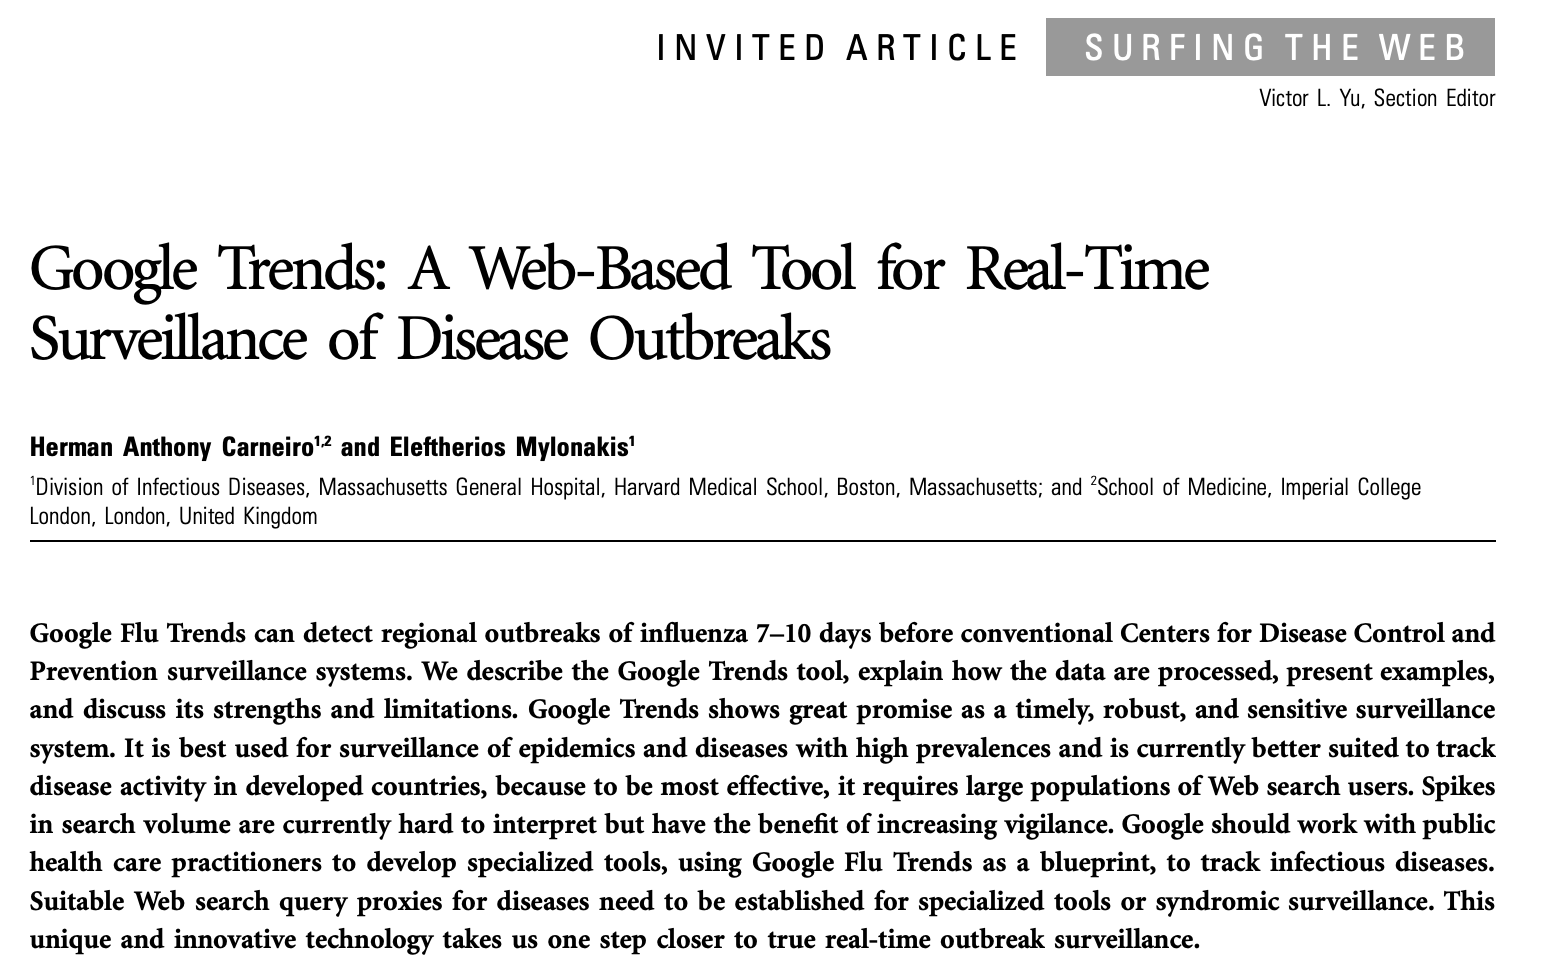
\includegraphics[width=\textwidth]{fig-7-trends/gtrends-flu.png}
    \end{figure}
\end{frame}

\begin{frame}{Google Trends -- przykłady}
    \begin{figure}
        \centering
        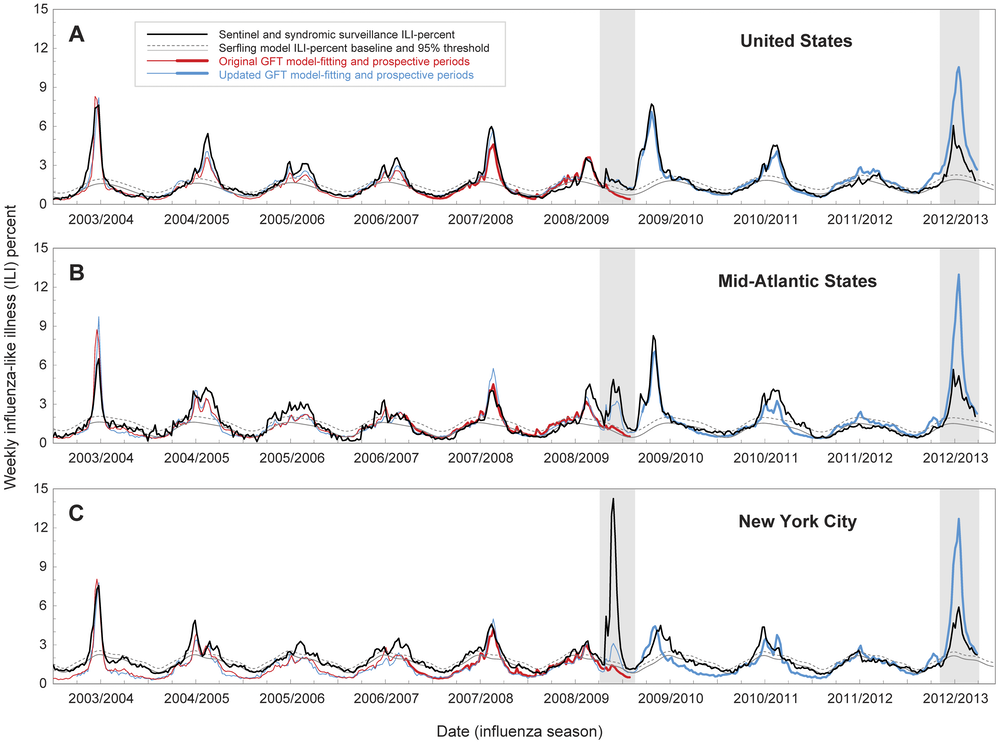
\includegraphics[width=0.8\textwidth]{fig-7-trends/gtrends-flu-2.png}
    \end{figure}
\end{frame}

\begin{frame}{Google Trends -- przykłady}
    \begin{figure}
        \centering
        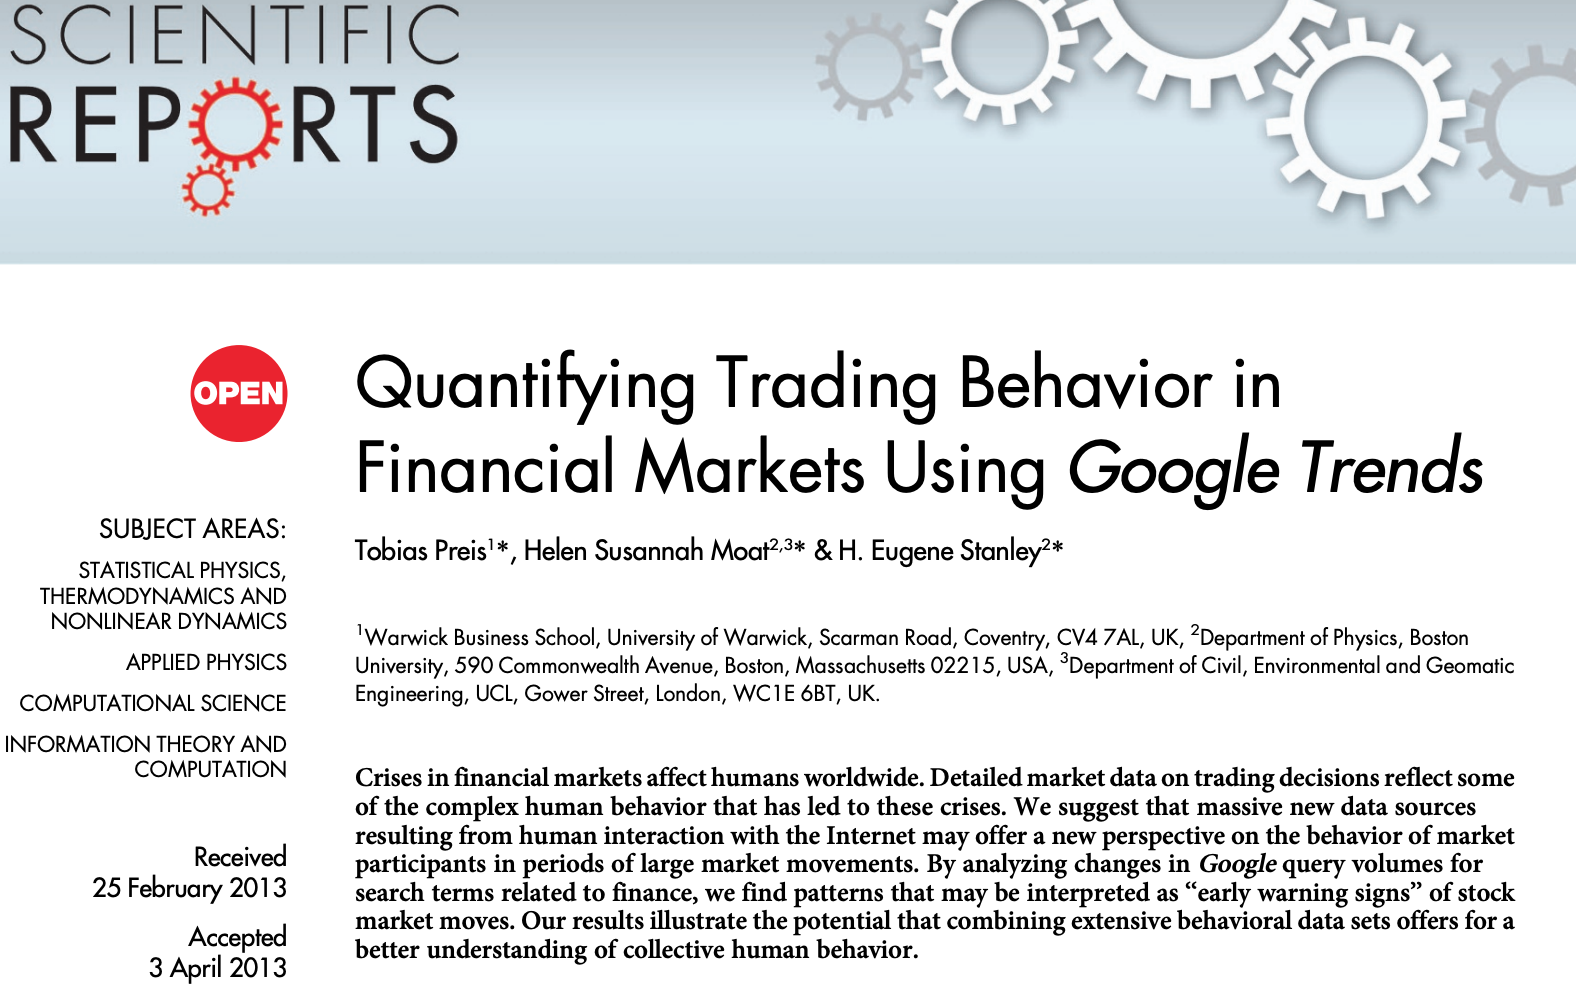
\includegraphics[width=\textwidth]{fig-7-trends/gtrends-paper2.png}
    \end{figure}
\end{frame}

\begin{frame}{Google Trends -- przykłady}
    \begin{figure}
        \centering
        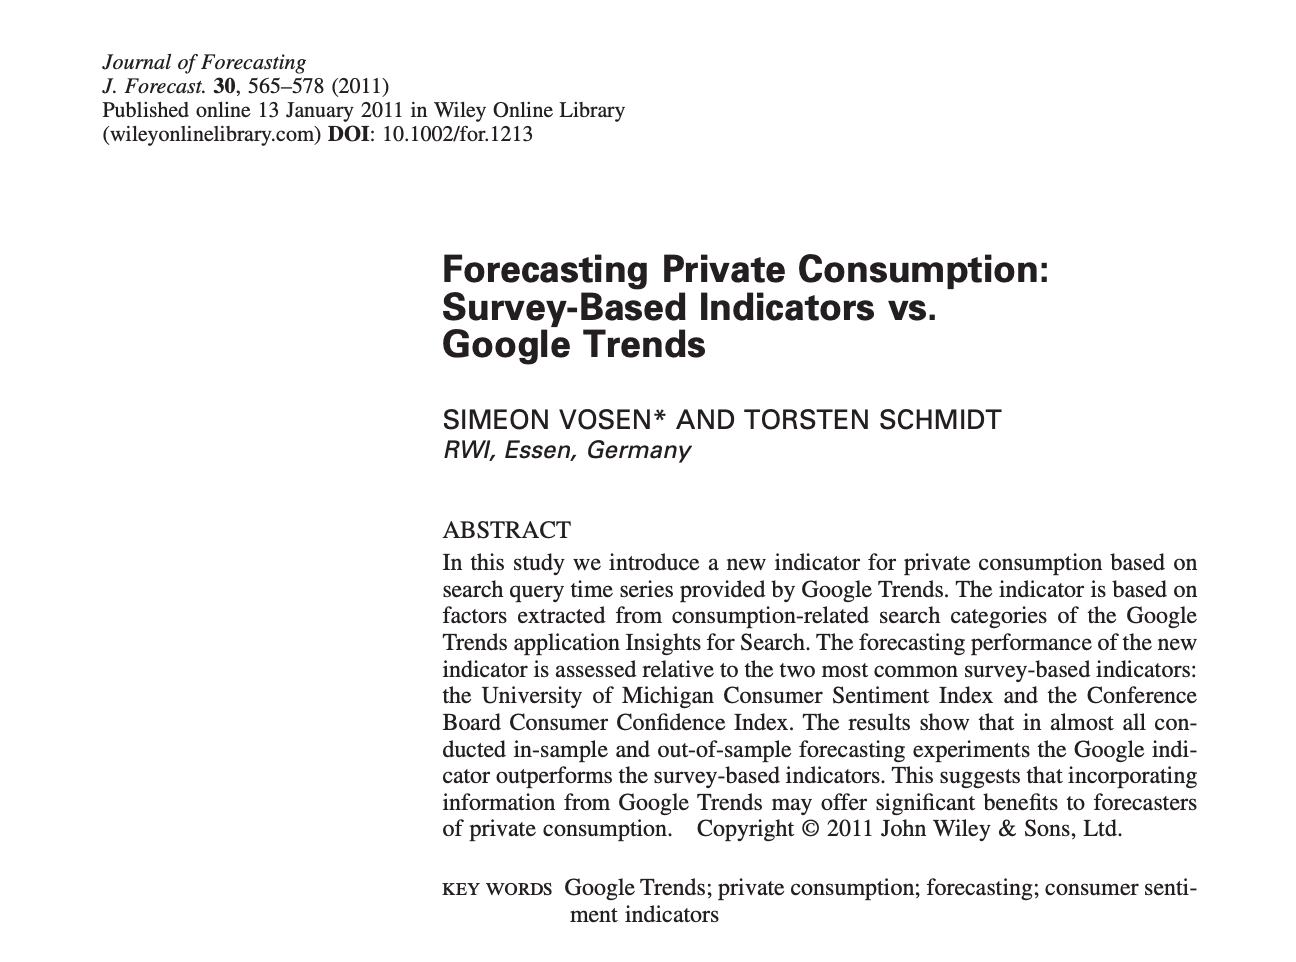
\includegraphics[width=\textwidth]{fig-7-trends/gtrends-paper3.png}
    \end{figure}
\end{frame}

\begin{frame}{Google Trends -- nauka}
    \begin{figure}
        \centering
        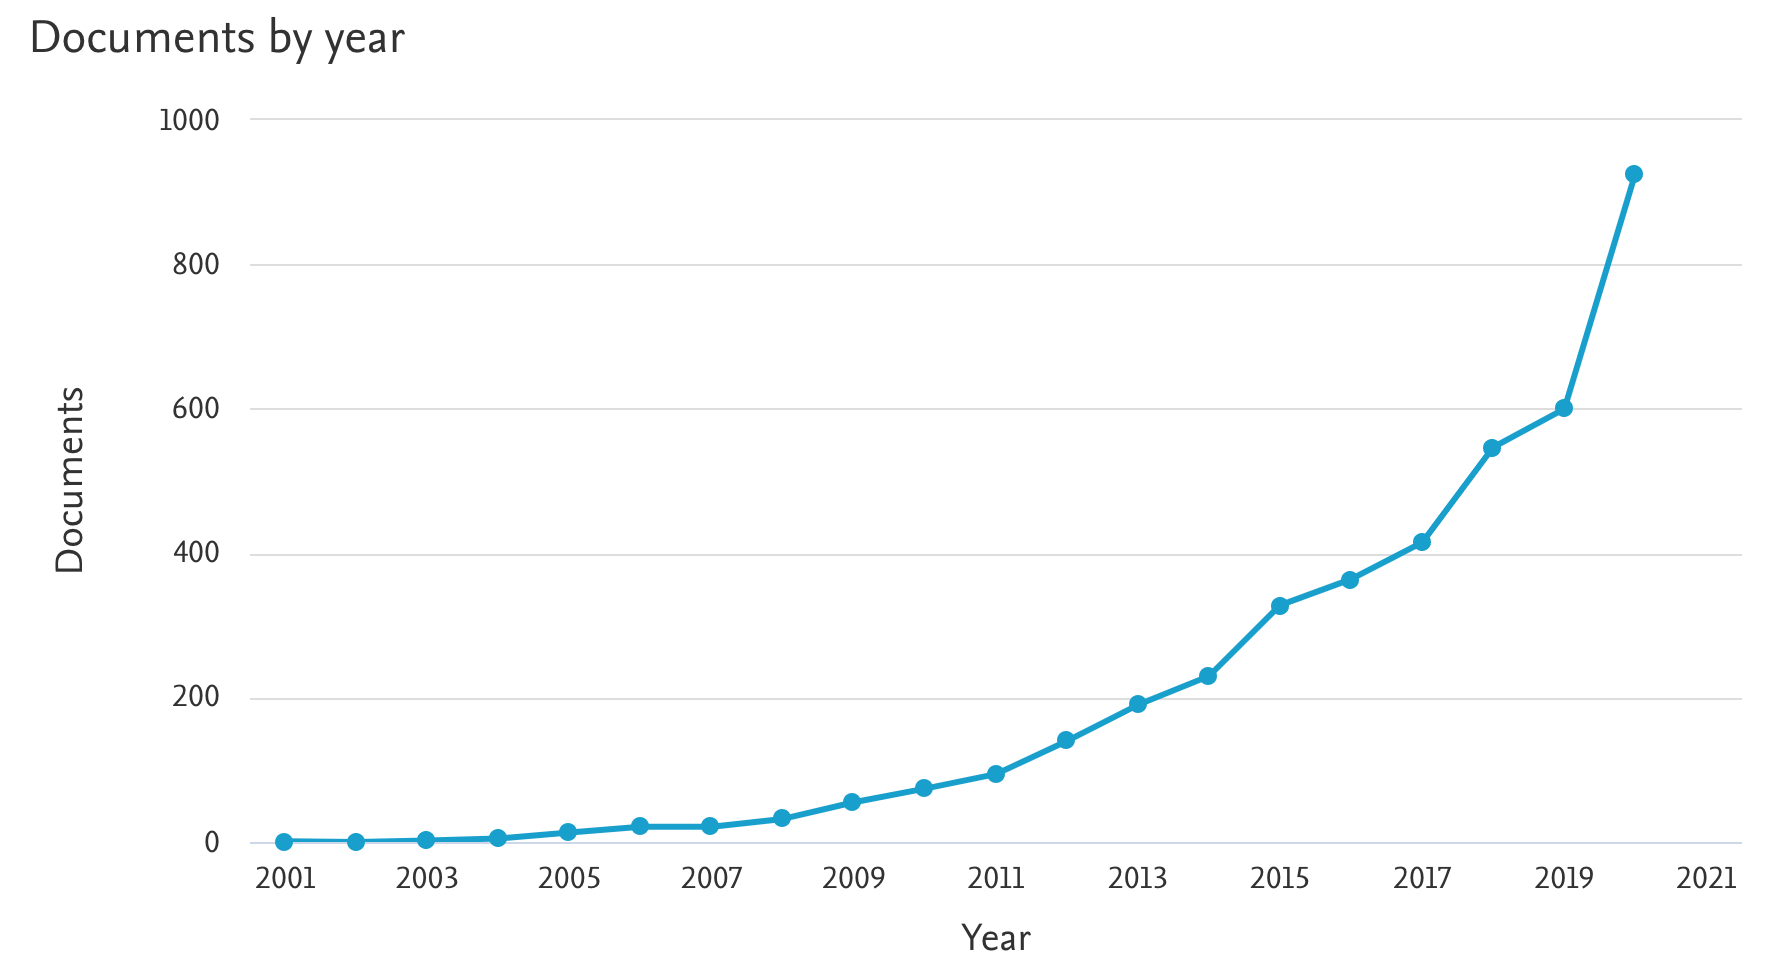
\includegraphics[width=\textwidth]{fig-7-trends/gtrends-scopus.png}
        \caption{Liczba artykułów naukowych indeksowanych w bazie Scopus zawierająca wyrażenie "Google Trends"}
    \end{figure}
\end{frame}

\begin{frame}{Google Trends -- nauka}
    \begin{figure}
        \centering
        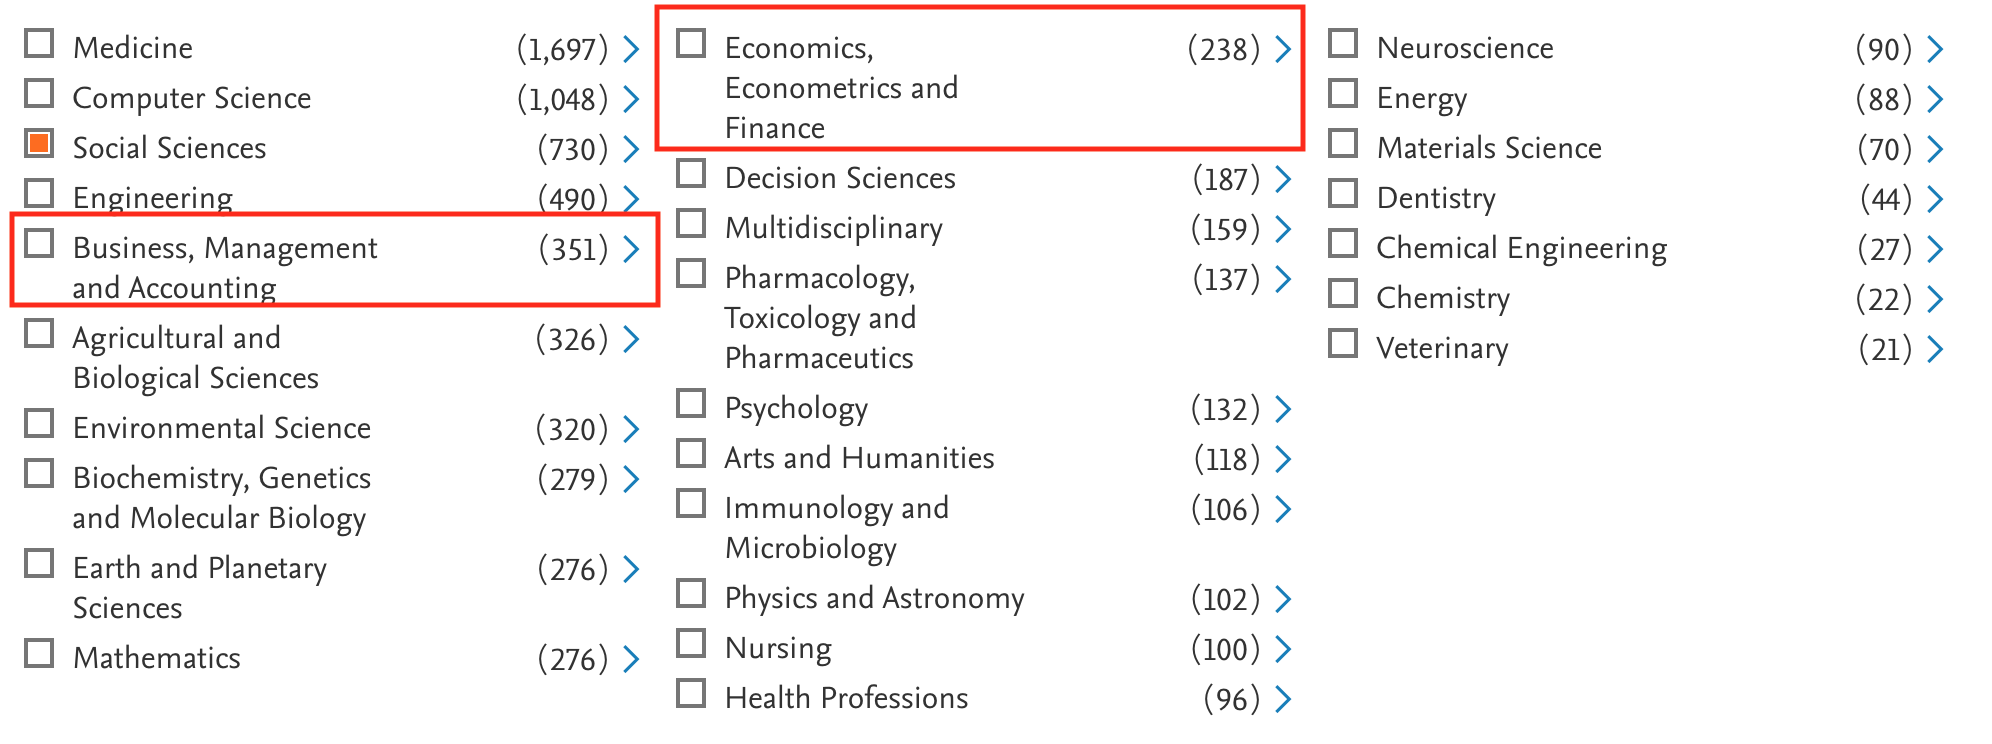
\includegraphics[width=\textwidth]{fig-7-trends/gtrends-scopus-2.png}
        \caption{Liczba artykułów naukowych indeksowanych w bazie Scopus zawierająca wyrażenie "Google Trends" według dziedziny}
    \end{figure}
\end{frame}


\begin{frame}{Google Trends -- COVID19}
    \begin{figure}
        \centering
        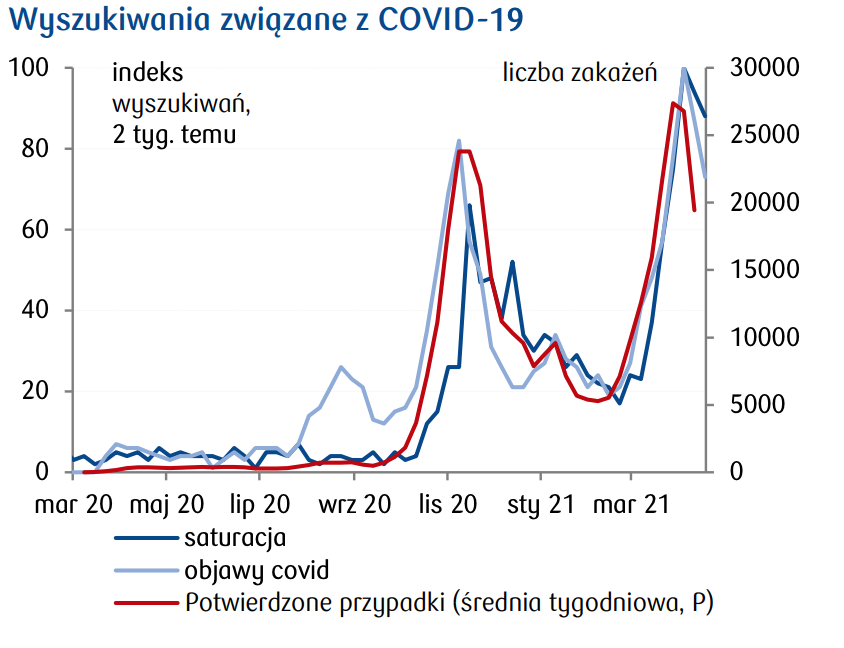
\includegraphics[width=0.8\textwidth]{fig-7-trends/gtrends-covid.png}
        \caption{Zestawienie przygotowane przez zespół PKO PB Research}
    \end{figure}
\end{frame}

\begin{frame}{Google Trends -- podsumowanie}
Ogólnie możemy podsumować korzystanie z Google Trends następujaco:

\begin{itemize}
    \item wykorzystanie indeksu Google Trends jako zmiennej w modelach prognostycznych (prognozowanie krótkookresowe, nowcasting),
    \item wykorzystanie indeksu Google Trends w modelach przekrojowych / panelowych dodatkowe zmienne wyjaśniające dane zjawisko.
\end{itemize}

\end{frame}


\begin{frame}{Google Trends -- jak korzystać?}
Mamy dwie możliwości korzystania z Google Trends:
\begin{itemize}
\item oficjalna strona Google Trends: \url{https://trends.google.com/trends/?geo=PL}
\item pakiety w językach programowania: \texttt{gtrendsR} (w R), \texttt{pytrends} (w Python).
\end{itemize}

\end{frame}

\begin{frame}{Google Trends -- przykład}
    \begin{center}
        Przejdźmy do przykładu.
    \end{center}
\end{frame}




\section{Web scraping}

\begin{frame}{Czym jest web scraping?}
\begin{itemize}
    \item Jest to metoda wykorzystywanych do automatycznego pobierania i ekstrakcji zawartości stron stron internetowych (niezależnie od stosowanej technologii).
    \item W tym kontekście należy rozróżnić: \textit{web crawling}, który polega na indeksowaniu stron/portali internetowych, a \textit{web scraping}, który polega na ekstrakcji informacji z tych stron.
    \item Głównym elementem tej metody jest odpowiedni algorytm (tzw. \textit{scraper}), który w małym (np. dopasowany do jednego portalu) lub dużym (np. rozpoznaje zwartość) stopniu działa automatycznie.
    \item Tożsame pojęcia: \textit{Web scraping}, \textit{web harvesting}, czy \textit{web data extraction}
    \item Podstawowe technologie: WWW, html, przeglądarka internetowa.
\end{itemize}
\end{frame}

\begin{frame}{Czym jest web scraping? -- idea}
\begin{center}
    
\includegraphics[width=0.7\textwidth]{fig-5-web/otodom.png}
\end{center}
\end{frame}

\begin{frame}{Web scraping w ekonomii -- przykłady}
    Wybrane publikacje:
    \begin{itemize}
    \small
        \item Edelman, B. (2012). Using internet data for economic research. Journal of Economic Perspectives, 26(2), 189-206.
        \item Cavallo, A. (2013). Online and official price indexes: Measuring Argentina's inflation. Journal of Monetary Economics, 60(2), 152-165.
        \item Cavallo, A., \& Rigobon, R. (2016). The billion prices project: Using online prices for measurement and research. Journal of Economic Perspectives, 30(2), 151-78.
        \item Hoekstra, R., ten Bosch, O., \& Harteveld, F. (2012). Automated data collection from web sources for official statistics: First experiences. Statistical Journal of the IAOS, 28(3, 4), 99-111.
        \item Beręsewicz, M., Białkowska, G., Marcinkowski, K., Maślak, M., Opiela, P., Pater, R., \& Zadroga, K. (2021). Enhancing the Demand for Labour survey by including skills from online job advertisements using model-assisted calibration. Survey Reseach Methods (forthcoming)
        \item Hołda, M. (2019). Newspaper-based economic uncertainty indices for Poland. Narodowy Bank Polski.
    \end{itemize}
\end{frame}

\begin{frame}{Web scraping w ekonomii -- przykłady}
\begin{figure}
    \centering
    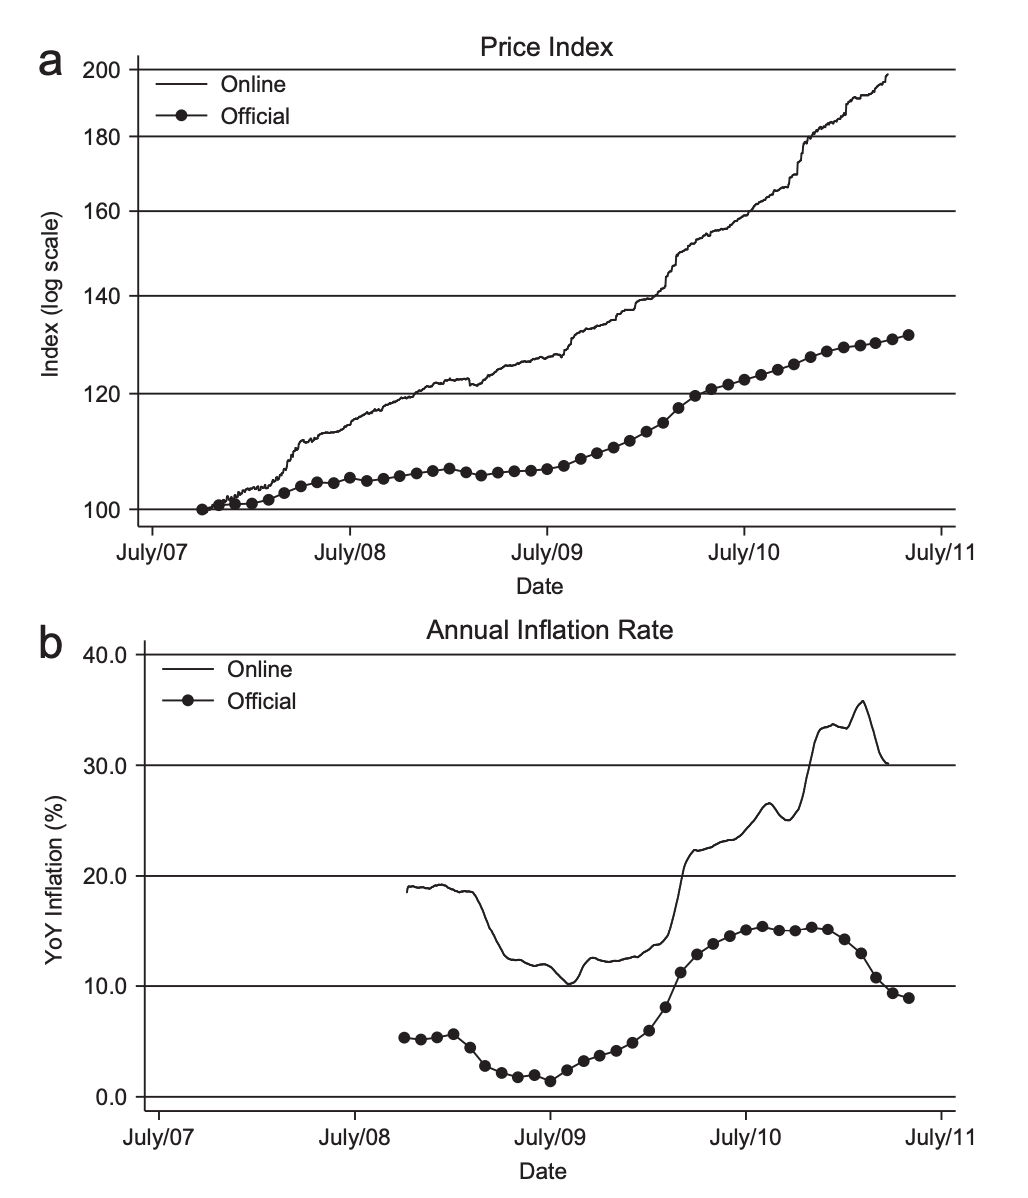
\includegraphics[width=0.5\textwidth]{fig-5-web/bpp-argentina.png}
    \caption{Źródło: Cavallo, A. (2013)}
    \label{fig:my_label}
\end{figure}
\end{frame}

\begin{frame}{Web scraping w ekonomii -- przykłady}
\begin{figure}
    \centering
    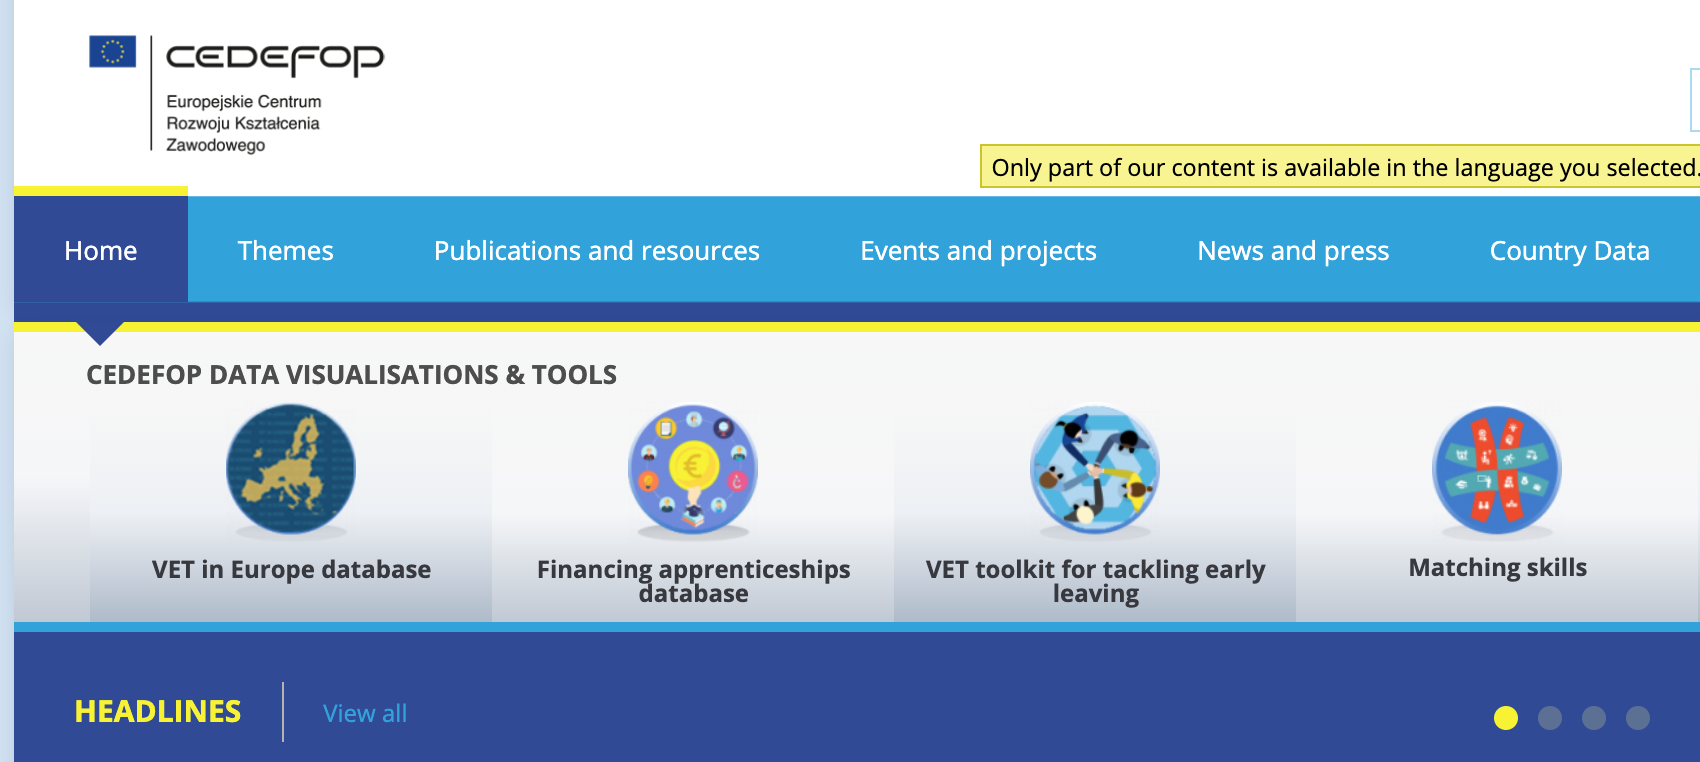
\includegraphics[width=\textwidth]{fig-5-web/cedefop.png}
    \caption{Źródło: Cedefop}
    \label{fig:my_label}
\end{figure}
\end{frame}

\begin{frame}{Web scraping w ekonomii -- przykłady}
\begin{figure}
    \centering
    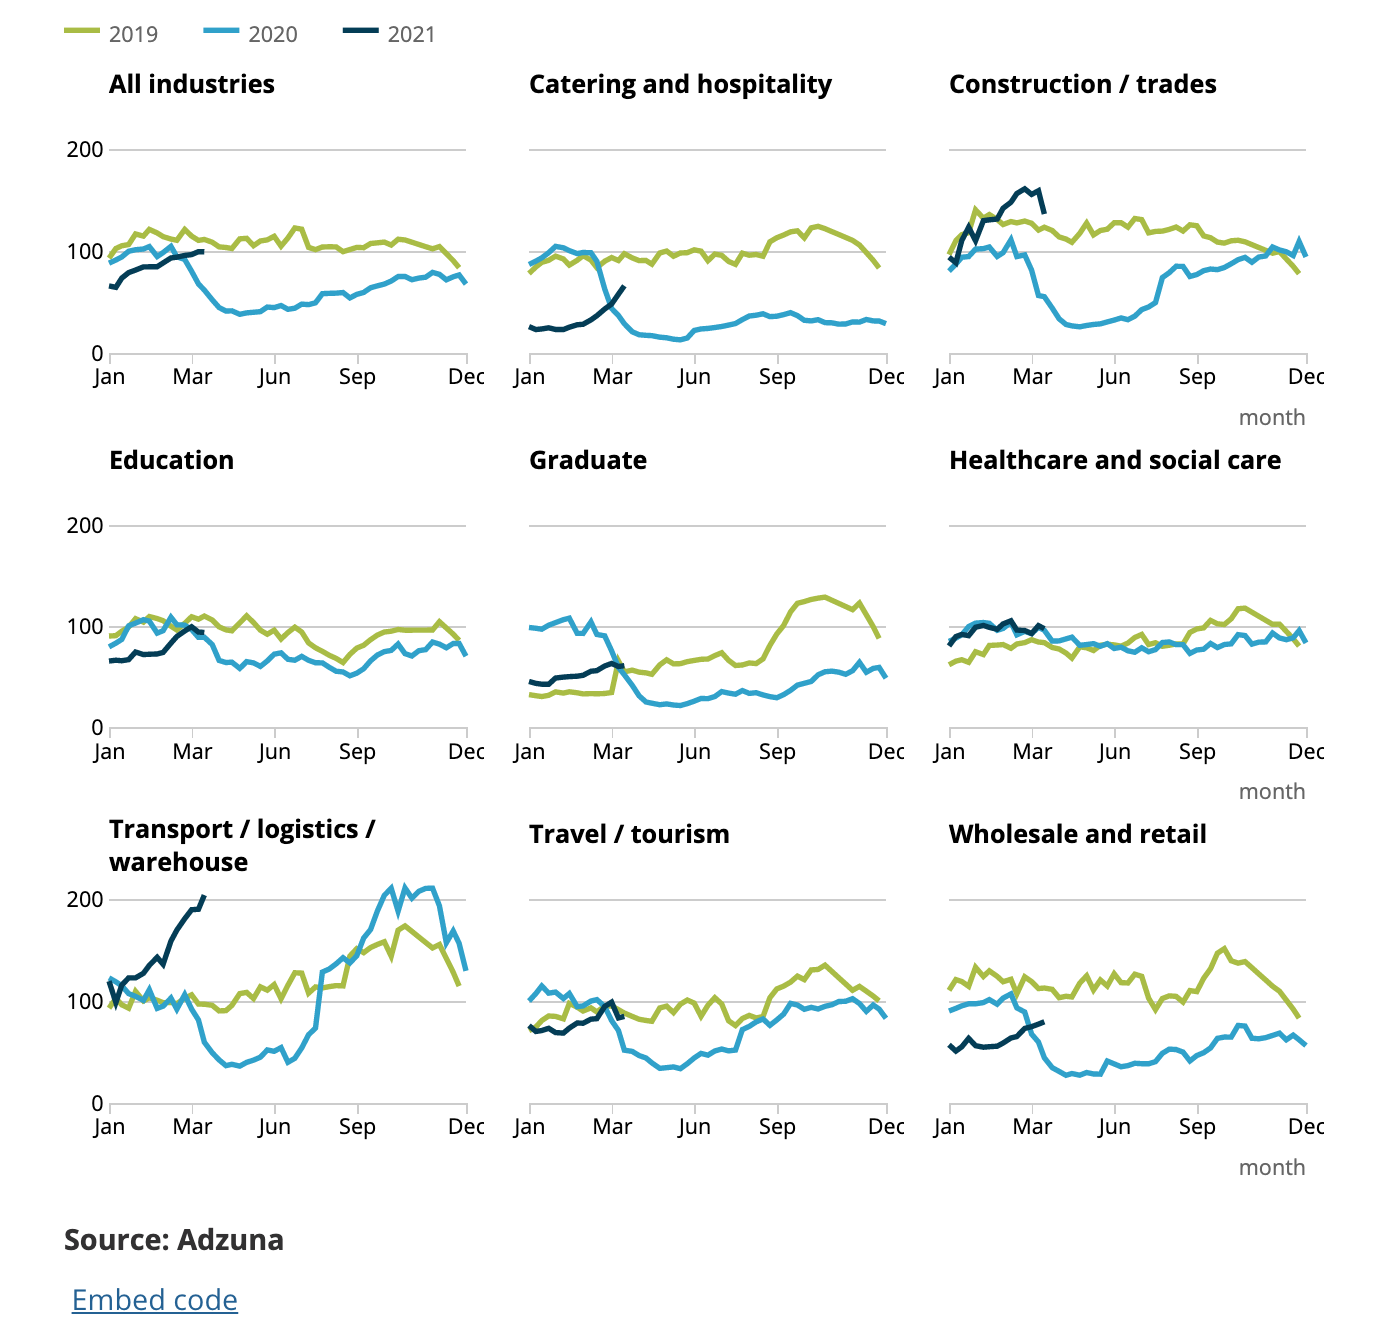
\includegraphics[width=0.5\textwidth]{fig-5-web/ons-jobs.png}
    \caption{Źródło: UK ONS -- Coronavirus and the latest indicators for the UK economy and society: 22 April 2021}
    \label{fig:my_label}
\end{figure}
\end{frame}


\begin{frame}{Web scraping w ekonomii -- przykłady}
\begin{figure}
    \centering
    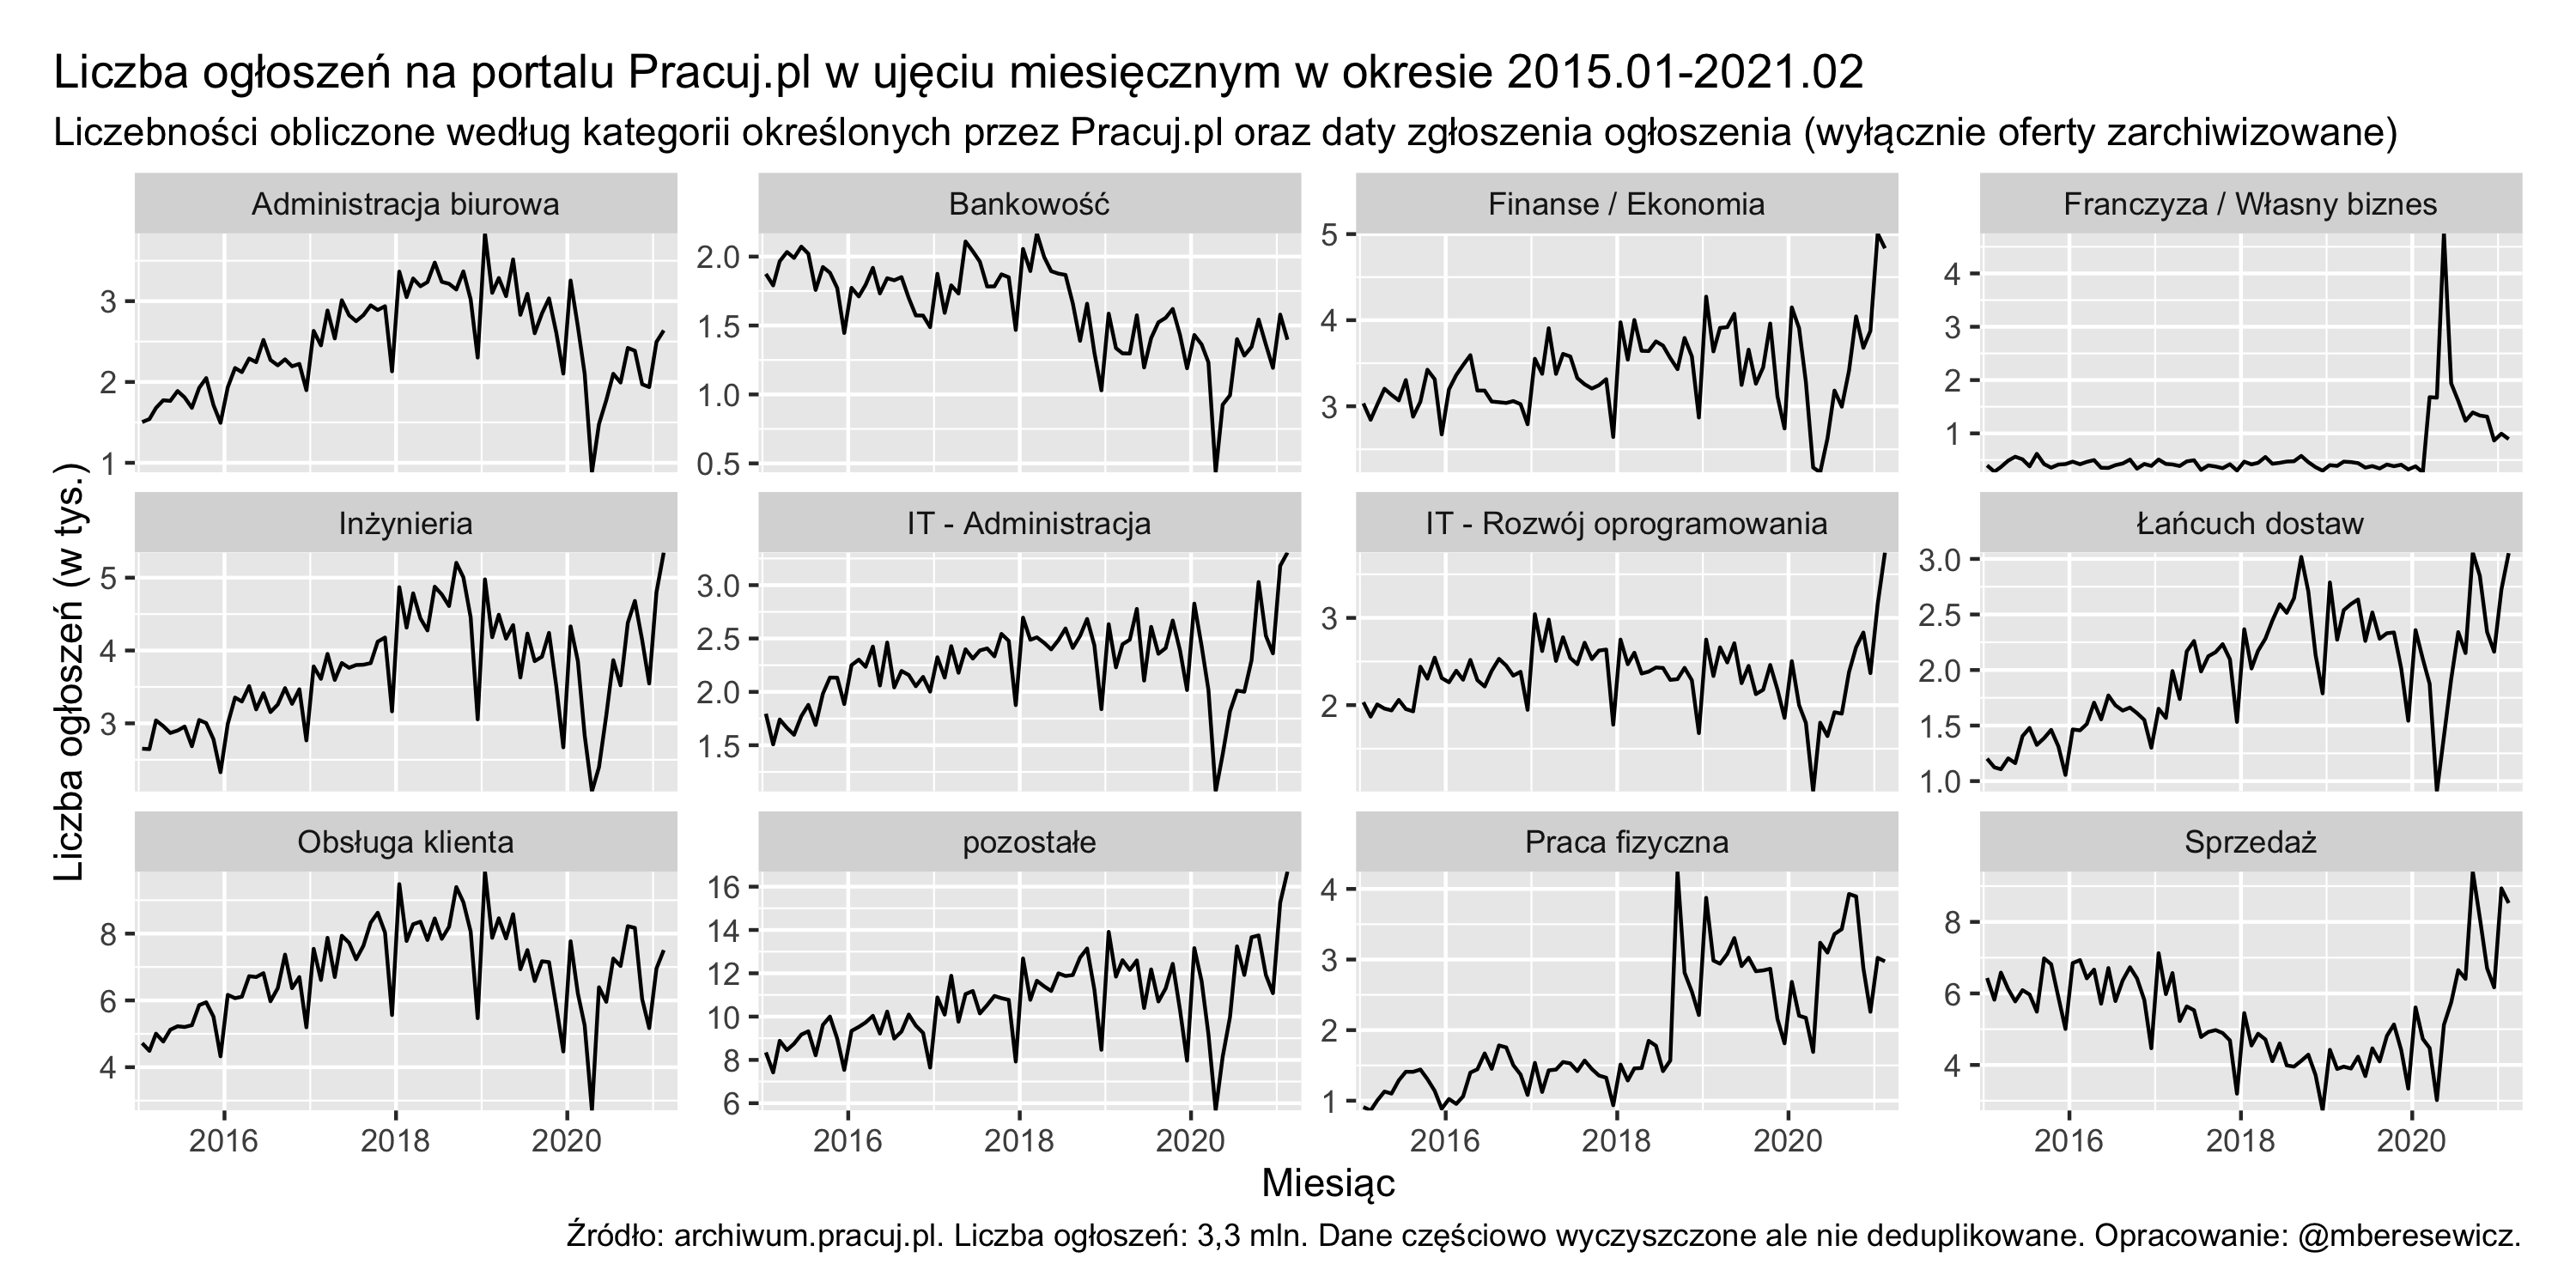
\includegraphics[width=\textwidth]{fig-5-web/oferty.png}
    \caption{Źródło: Opracowanie własne na podstawie pracuj.pl}
    \label{fig:my_label}
\end{figure}
\end{frame}

\begin{frame}{Web scraping w ekonomii -- przykłady}
\begin{figure}
    \centering
    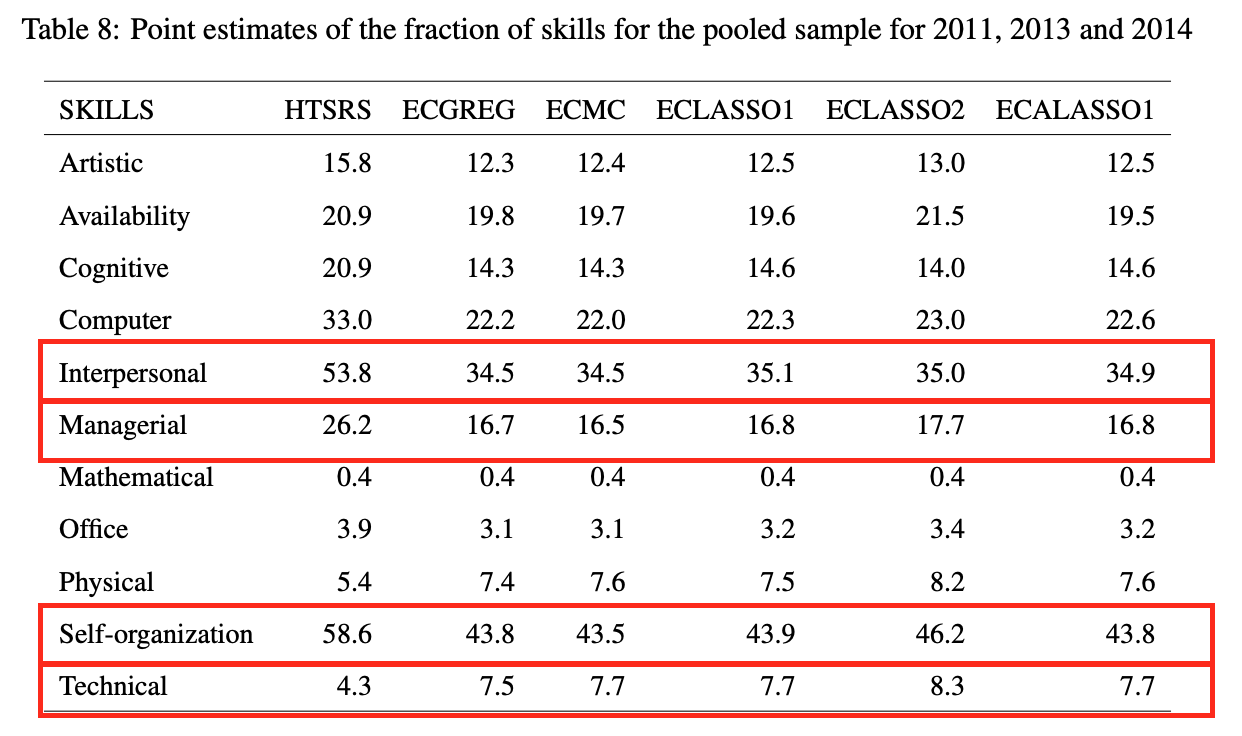
\includegraphics[width=\textwidth]{fig-5-web/beresewicz-tab.png}
    \caption{Źródło: Beręsewicz et al. (2021)}
    \label{fig:my_label}
\end{figure}
\end{frame}


\begin{frame}{Web scraping w ekonomii -- podsumowanie}
    Ogromna liczba zastosowań:
    \begin{itemize}
        \item mierniki ekonomii w czasie rzeczywistym (np. oferty pracy, nieruchomości, nastroje społeczne),
        \item weryfikacja różnych ekonomicznych konceptów (np. lepkość cen),
        \item now-casting / prognozowanie,
        \item rozszerzenie istniejących źródeł danych o informacje zawarte na portalach internetowych (np. popyt na pracę, RCiWN),
        \item zastąpienie wywiadów automatycznym pobieraniem informacji ze stron internetowych (np. pytanie o posiadanie social media, sklepu internetowego),
        \item aktualizacja operatów losowania (np. weryfikacja czy firma działa),
        \item wiele innych.
    \end{itemize}
\end{frame}

\begin{frame}{Web scraping -- wybrane technologie}
Słowo wstępu:
\begin{itemize}
    \item strony statyczne (HTML) vs dynamiczne (JavaScript),
    \item web scraping, a dostęp przez Application Programming Interface (API).
\end{itemize}

Przydatne biblioteki:
    \begin{itemize}
        \item Python -- \texttt{beautifulsoup}, \texttt{scrapy},
        \item R -- \texttt{rvest},
        \item Ogólne -- \texttt{PhantomJS}.
    \end{itemize}
\end{frame}

\begin{frame}{Web scraping -- przykład}
    \begin{center}
        Przejdźmy do przykładu w R.
    \end{center}
\end{frame}

\section{Reprezentatywność}

\subsubsection{Reprezentatywność -- definicje, pomiar, problematyka}


% % \begin{frame}{Quiz -- 3 minuty}

% % \begin{center}
% % \large

% %     Której wersji bardziej Państwo zaufacie?
    
% %     \vspace{0.5cm}
    
% %     \begin{enumerate}
% %         \item 1\% próbie losowej z 60\% realizacją (odsetkiem odpowiedzi), czy 
% %         \item rejestrowi administracyjnemu tworzonemu przez dobrowolne deklaracje (\textit{a self-reported administrative dataset.}) pokrywającym 80\% populacji?
% %     \end{enumerate}

% %     \vspace{0.5cm}
    
% %     \fbox{Quiz: \url{www.menti.com}, kod: 1659 4896}
% % \end{center}

% % \end{frame}


\begin{frame}{Zadanie -- 5 minut}

\begin{center}
\large

    Której wersji bardziej Państwo zaufacie? Dlaczego?
    
    \vspace{0.5cm}
    
    \begin{enumerate}
        \item 1\% próbie losowej z 60\% realizacją (odsetkiem odpowiedzi), czy 
        \item rejestrowi administracyjnemu tworzonemu przez dobrowolne deklaracje (\textit{a self-reported administrative dataset}) pokrywającym 80\% populacji?
    \end{enumerate}
\end{center}
\end{frame}

\begin{frame}{Zadanie -- 5 minut}
\begin{center}
\large
    Co oznacza reprezentatywność? Jak to Państwo rozumiecie? 
\end{center}
\end{frame}


\begin{frame}{Mocne prawo wielkich liczb}

Dla ciągów (całkowalnych) zmiennych losowych wprowadza się definicję spełniania przez nich tzw. mocnego (i słabego) prawa wielkich liczb.

Ciąg zmiennych niezależnych zmiennych losowych $\left(X_{n}\right)_{n=1}^{\infty}$ spełnia mocne prawo wielkich liczb (MPWL), gdy

\begin{equation}
\frac{1}{n} \sum_{k=1}^{n}\left(X_{k}-\mathrm{E} (X_{k})\right) \stackrel{p . n .}{\longrightarrow} 0
\end{equation}

p.n. (Prawie na pewno): określenie zdarzenia zachodzącego z pra\-wdo\-po\-do\-bień\-stwem 1. Sformułowanie to pojawia się w naturalny sposób np. przy badaniu zagadnień granicznych.
\end{frame}

\begin{frame}{Estymator -- własności}

Niech $\hat{\theta}=T(X_1,X_2,...,X_n)$ będzie estymatorem parametru $\theta$, to

    \begin{itemize}
        \item estymator jest nieobciążony gdy
        \begin{equation}
            E(\hat{\theta}) = \theta,
        \end{equation}
        \item obciążenie estymatora oznaczamy przez
        \begin{equation}
            B(\hat{\theta}) = E(\hat{\theta}) - \theta,
        \end{equation}
        \item wariancję estymatora natomiast
        \begin{equation}
            D^2(\hat{\theta}) = E(\hat{\theta} - E(\hat{\theta}))^2,
        \end{equation}
        \item estymator jest zgodny, gdy zachodzi
        \begin{equation}
        \lim_{n \rightarrow \infty} P \left( |\hat{\theta}_n - \theta| \leq \epsilon \right) = 1.
        \end{equation}
    \end{itemize}
\end{frame}

\begin{frame}{Mała, a duża próba -- The 1936 Literary Digest Poll}
    \begin{figure}
        \centering
        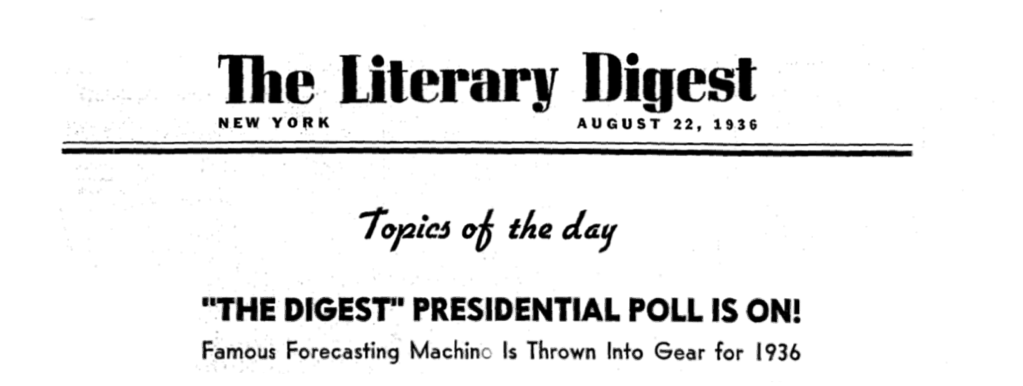
\includegraphics[width=\textwidth]{fig-2-definicje/digest.png}
    \end{figure}
\end{frame}

\begin{frame}{Mała, a duża próba -- The 1936 Literary Digest Poll}
    \begin{itemize}
        \item The Literary Digest był bardzo wpływowym, amerykańskim tygodnikiem.
        \item Od 1916 roku poprawnie przewidywał wyniki wyborów w USA, a w \textbf{1936 roku odbywały się ważne wybory między Rooseveltem, a Landonem}.
        \item Tygodnik wysłał ponad \textbf{10 mln} karty do głosowania, a ponad \textbf{2.4 mln} kart zostało odesłanych.
            \begin{itemize}
                \item \textit{The mailing list was “drawn from every telephone book in the United States, from the rosters of clubs and associations, from city directories, lists of registered voters, classified mail-order and occupational data” (Lohr and Brick (2017))}
            \end{itemize}
        \item Według tego badania wybory miał wygrać \textbf{Landon z 55\%} poparciem, a \textbf{Roosevelt} miał otrzymać\textbf{ 41\%}. 
         \item W tym samym czasie Instytut Gallup'a wykorzystując próbę wielkości 50 tys. prognozował \textbf{56\% dla Roosevelta}.
        \item Faktyczne wyniki były znacząco inne: \textbf{Roosevelt 61\%, Landon 37\%}.
        \item W 1938 roku Magazyn został zamknięty.
    \end{itemize}
\end{frame}

\begin{frame}{The 1936 Literary Digest Poll -- przyczyny}
    \begin{figure}
        \centering
        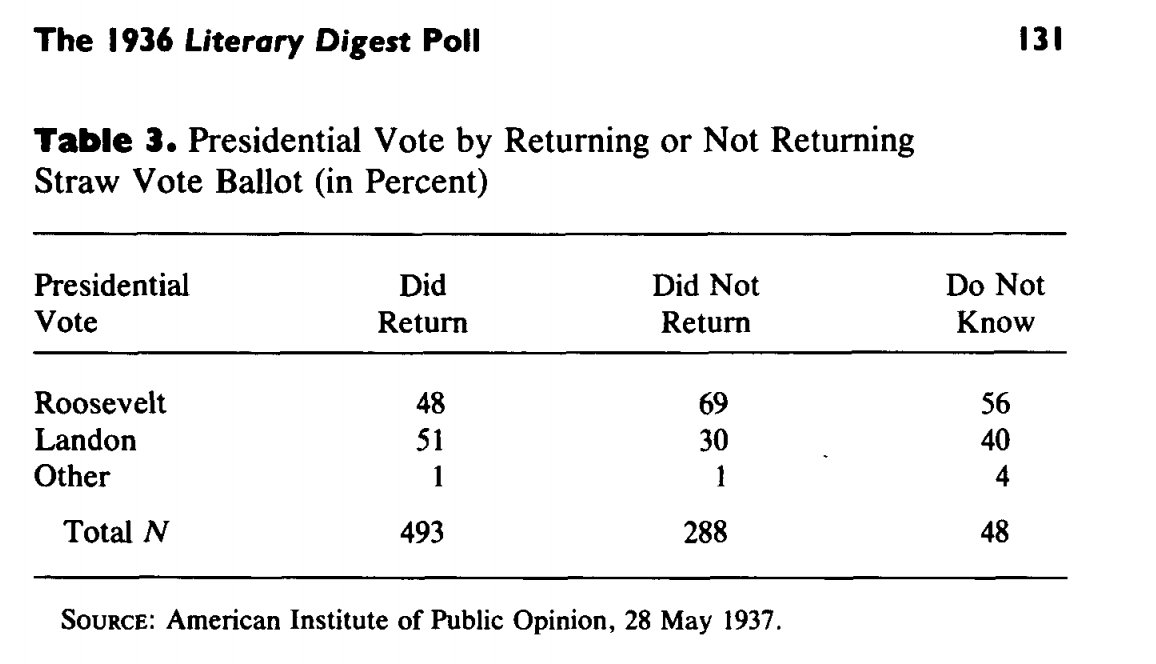
\includegraphics[width=\textwidth]{fig-2-definicje/digest-why.png}
        \caption{Źródło: Squire, P. (1988). Why the 1936 Literary Digest poll failed. Public Opinion Quarterly, 52(1), 125-133.}
        \label{fig:my_label}
    \end{figure}
\end{frame}


\begin{frame}{Przykłady}

Reprezentatywność w opisie badań, na przykład:

\begin{itemize}
    \justifying
    \item \textbf{Badanie EU-SILC} jest dobrowolnym, `reprezentacyjnym` badaniem ankietowym prywatnych gospodarstw domowych, realizowanym techniką bezpośredniego wywiadu z respondentem.
    \item \textbf{Badanie Aktywności Ekonomicznej Ludności} przeprowadzane jest `metodą reprezentacyjną`, a wyniki badania uogólniane są na populację generalną. Z uwagi na reprezentacyjną metodę badania zalecana jest ostrożność w posługiwaniu się danymi w tych przypadkach, gdy zastosowano bardziej szczegółowe podziały i występują liczby niskiego rzędu (mniejsze niż 15 tys.). 
\end{itemize}
\end{frame}


\begin{frame}{Reprezentatywność -- definicja}
Za słownikiem PWN (źródło: \url{http://sjp.pwn.pl/sjp/reprezentatywny;2515040.html})

\begin{itemize}
    \item \textbf{reprezentatywny} «mający cechy charakterystyczne dla jakiejś zbiorowości» (reprezentatywnie, reprezentatywność)
\end{itemize}


\end{frame}

\begin{frame}{Reprezentatywność -- Próba reprezentatywna}

\textbf{Próba reprezentatywna}

\begin{itemize}
    \item Próba, której struktura ze względu na badane cechy (zmienne) jest zbliżona do struktury populacji statystycznej, z której pochodzi. 
    \item Reprezentatywność próby (próba reprezentatywna) można uzyskać stosując zarówno losowe (probabilistyczne) jak i nielosowe (nieprobabilistyczne) techniki wyboru próby. 
    \item Należy jednak zaznaczyć, iż większą szansę na reprezentatywność próby daje zastosowanie technik losowego jej wyboru.
\end{itemize}

\vspace{0.5cm}

Źródło: \url{https://stat.gov.pl/metainformacje/slownik-pojec/pojecia-stosowane-w-statystyce-publicznej/2771,pojecie.html}.
\end{frame}

\begin{frame}{Reprezentatywność -- losowy dobór (za GUS)}
 
\textbf{Losowy wybór próby}

Technika pobierania próby z badanej populacji generalnej, która spełnia dwa następujące warunki: 
\begin{enumerate}
    \item każda jednostka populacji ma dodatnie i znane prawdopodobieństwo dostania się do próby; 
    \item dla każdego zespołu jednostek populacji można ustalić prawdopodobieństwo tego, że w całości znajdzie się on w próbie. 
\end{enumerate}

\vspace{0.5cm}

\textbf{Próba losowa}

Próba pobrana za pomocą odpowiednich technik probabilistycznych (losowy wybór próby).

\vspace{0.5cm}

Źródło: \url{https://stat.gov.pl/metainformacje/slownik-pojec/pojecia-stosowane-w-statystyce-publicznej/2748,pojecie.html}.

\end{frame}


\begin{frame}{Reprezentatywność -- nielosowy dobór (za GUS)}

\textbf{Nielosowy wybór próby}

Technika wyboru próby, która nie spełnia choć jednego z dwóch warunków określonych w definicji losowego wyboru próby. 

Najpopularniejszymi technikami nielosowego wyboru próby są: wybór przypadkowy, wybór dogodny, wybór celowy i wybór kwotowy.

\vspace{0.5cm}

Źródło: \url{https://stat.gov.pl/metainformacje/slownik-pojec/pojecia-stosowane-w-statystyce-publicznej/2761,pojecie.html}.
\end{frame}

\begin{frame}{Definicja reprezentatywności}
    Kruskal i Mosteller (1979a, 1979b, 1979c), na podstawie ówczesnej przeglądu literatury, podali następujące definicje reprezentatywności:

\begin{itemize}
\justifying
\item ogólne, nieuzasadnione twierdzenie o danych  (ang. \textit{general, unjustified acclaim for the data})
\item losowy doboru do próby (ang. \textit{absence of selective forces})
\item miniatura populacji (ang. \textit{mirror or miniature of the population})
\item typowa jednostka (ang. \textit{typical or ideal case(s)})
\item pokrycie populacji (ang. \textit{coverage of the population})
\item termin bez uzasadnienia (ang. \textit{a~vague term to be made precise})
\item określona metoda doboru próby (ang. \textit{representative sampling as a~specific sampling method})
\item pozwala na nieobciążoną estymację (ang. \textit{representative sampling as permitting good estimation})
\item dobór próby odpowiedni do danego problemu (ang. \textit{representative sampling as good enough for a~particular purpose})
\end{itemize}
\end{frame}

\begin{frame}{Reprezentatywność -- źródła danych }
    \begin{enumerate}
        \item \textbf{Źródła statystyczne} -- źródła informacji statystycznej zaprojektowane przez statystyków i na potrzeby statystyki (np badania częściowe, spisy powszechne, rejestry statystyczne, sprawozdawczość przedsiębiorstw)
        \item \textbf{Źródła niestatystyczne} -- wszystkie pozostałe źródła danych, których celem nie jest dostarczanie informacji statystycznej o całej populacji (np. rejestry administracyjne, big data)
    \end{enumerate}
\end{frame}

\begin{frame}{Reprezentatywność -- źródła danych wg Citro (2014)}

% Constance Ann Forbes Citro (born June 9, 1942 in St. Louis, Missouri)[1] is an American political scientist and statistician. She is the former director of the Committee on National Statistics of the National Research Council, and works as a senior scholar for the Committee on National Statistics.[2]

\begin{columns}

\begin{column}{0.5\textwidth}
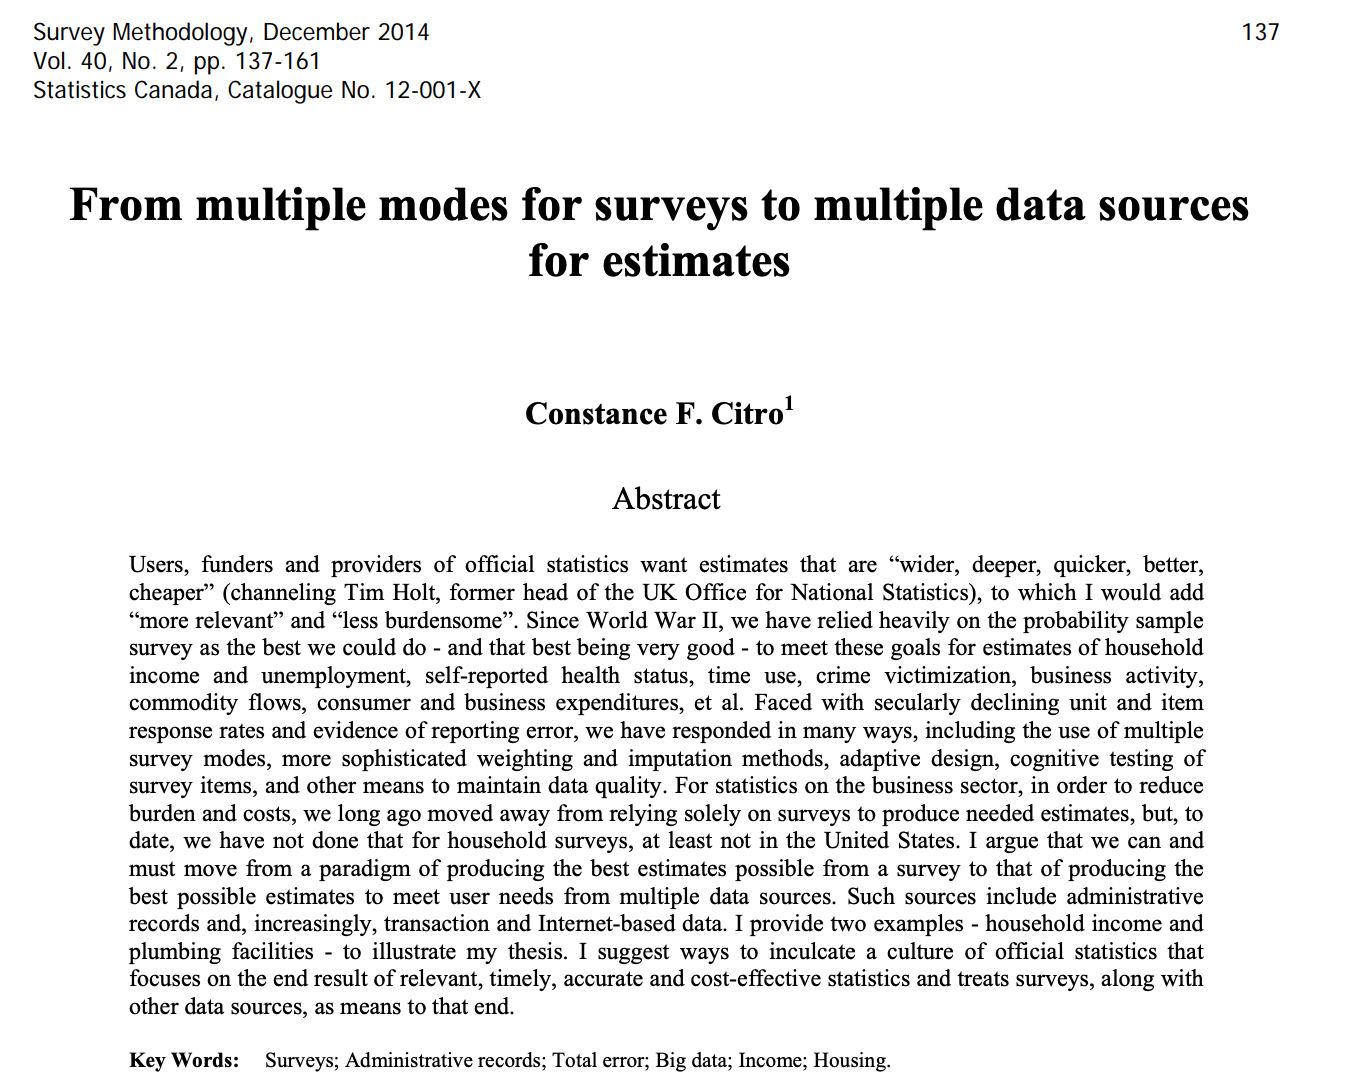
\includegraphics[width=\textwidth]{fig-2-definicje/citro1.png}
\end{column}

\begin{column}{0.5\textwidth}
\begin{itemize}
    \small
    \item \textbf{Constance Citro (ur. 1942)} -- amerykańska statystyczka i politolożka, m.in. była dyrektor \textit{the Committee on National Statistics of the National Research Council}.
\end{itemize}
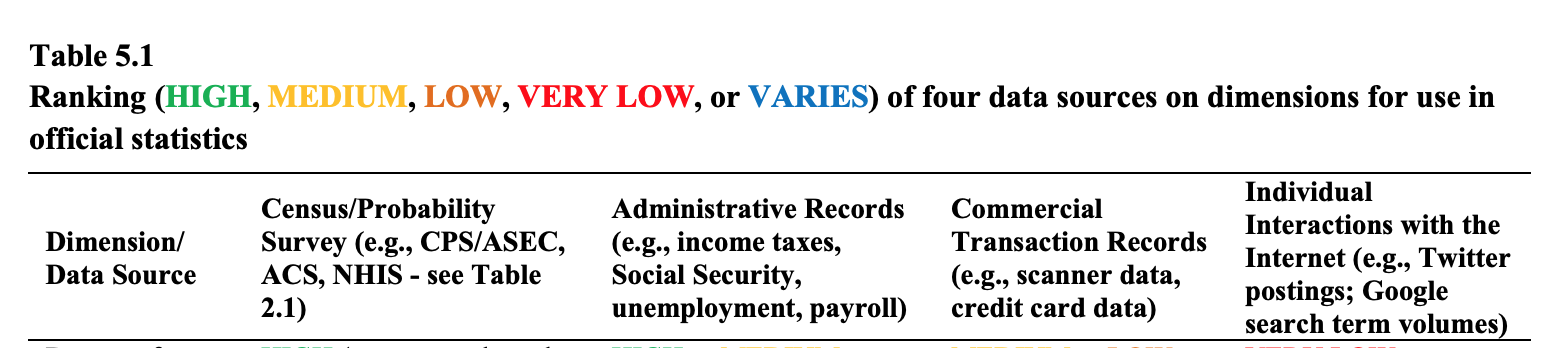
\includegraphics[width=\textwidth]{fig-2-definicje/citro2.png}
\end{column}

\end{columns}

\end{frame}




\begin{frame}{Przykłady -- Selectivv}
    
    \begin{itemize}

    \item Firma posiada obecnie największy w Europie Środkowo-Wschodniej zbiór informacji o właścicielach smartfonów i tabletów, \textbf{który obejmuje łącznie 82 mln osób, z czego 14 mln w Polsce}. \\
    
    
    \item Jesteśmy połączeni z sieciami reklamowymi, co daje nam dostęp do \textbf{200 tys. aplikacji i 15 milionów stron internetowych}. \\
    
    \item Średnio o jednym użytkowniku Selectivv \textbf{pozyskuje 362 informacje}, m.in. dane demograficzne, zainteresowania, jego styl życia oraz lokalizacje, w jakich przebywa. Wykorzystanie big data pozwoliło na wyróżnienie ponad 60 profili behawioralnych konsumentów, kategoryzując ich na m.in.: osoby planujące powiększenie rodziny, bywalców galerii handlowych, użytkowników bankowości mobilnej czy aplikacji muzycznych.
            
    \end{itemize}
\end{frame}

\begin{frame}{Przykłady -- banki}

\begin{figure}
    \centering
    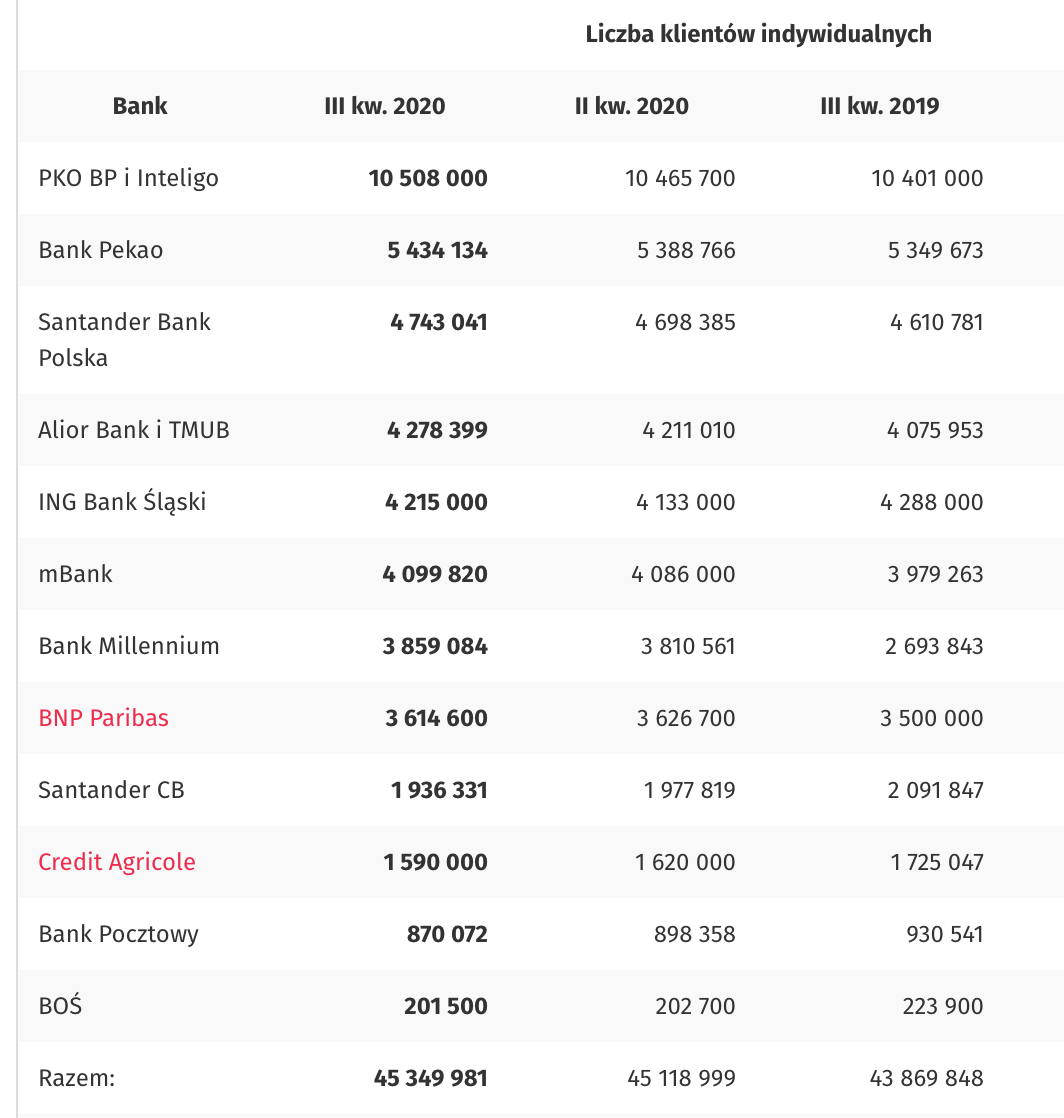
\includegraphics[width=0.5\textwidth]{fig-2-definicje/banki.png}
    \caption{Liczba indywidualnych klientów banków w Polsce w III kw. 2020}
\end{figure}
Źródło: \url{https://prnews.pl/raport-prnews-pl-liczba-klientow-w-bankach-iii-kw-2020-455068}    
\end{frame}

\begin{frame}{Przykład -- CBOP}
\begin{figure}
    \centering
    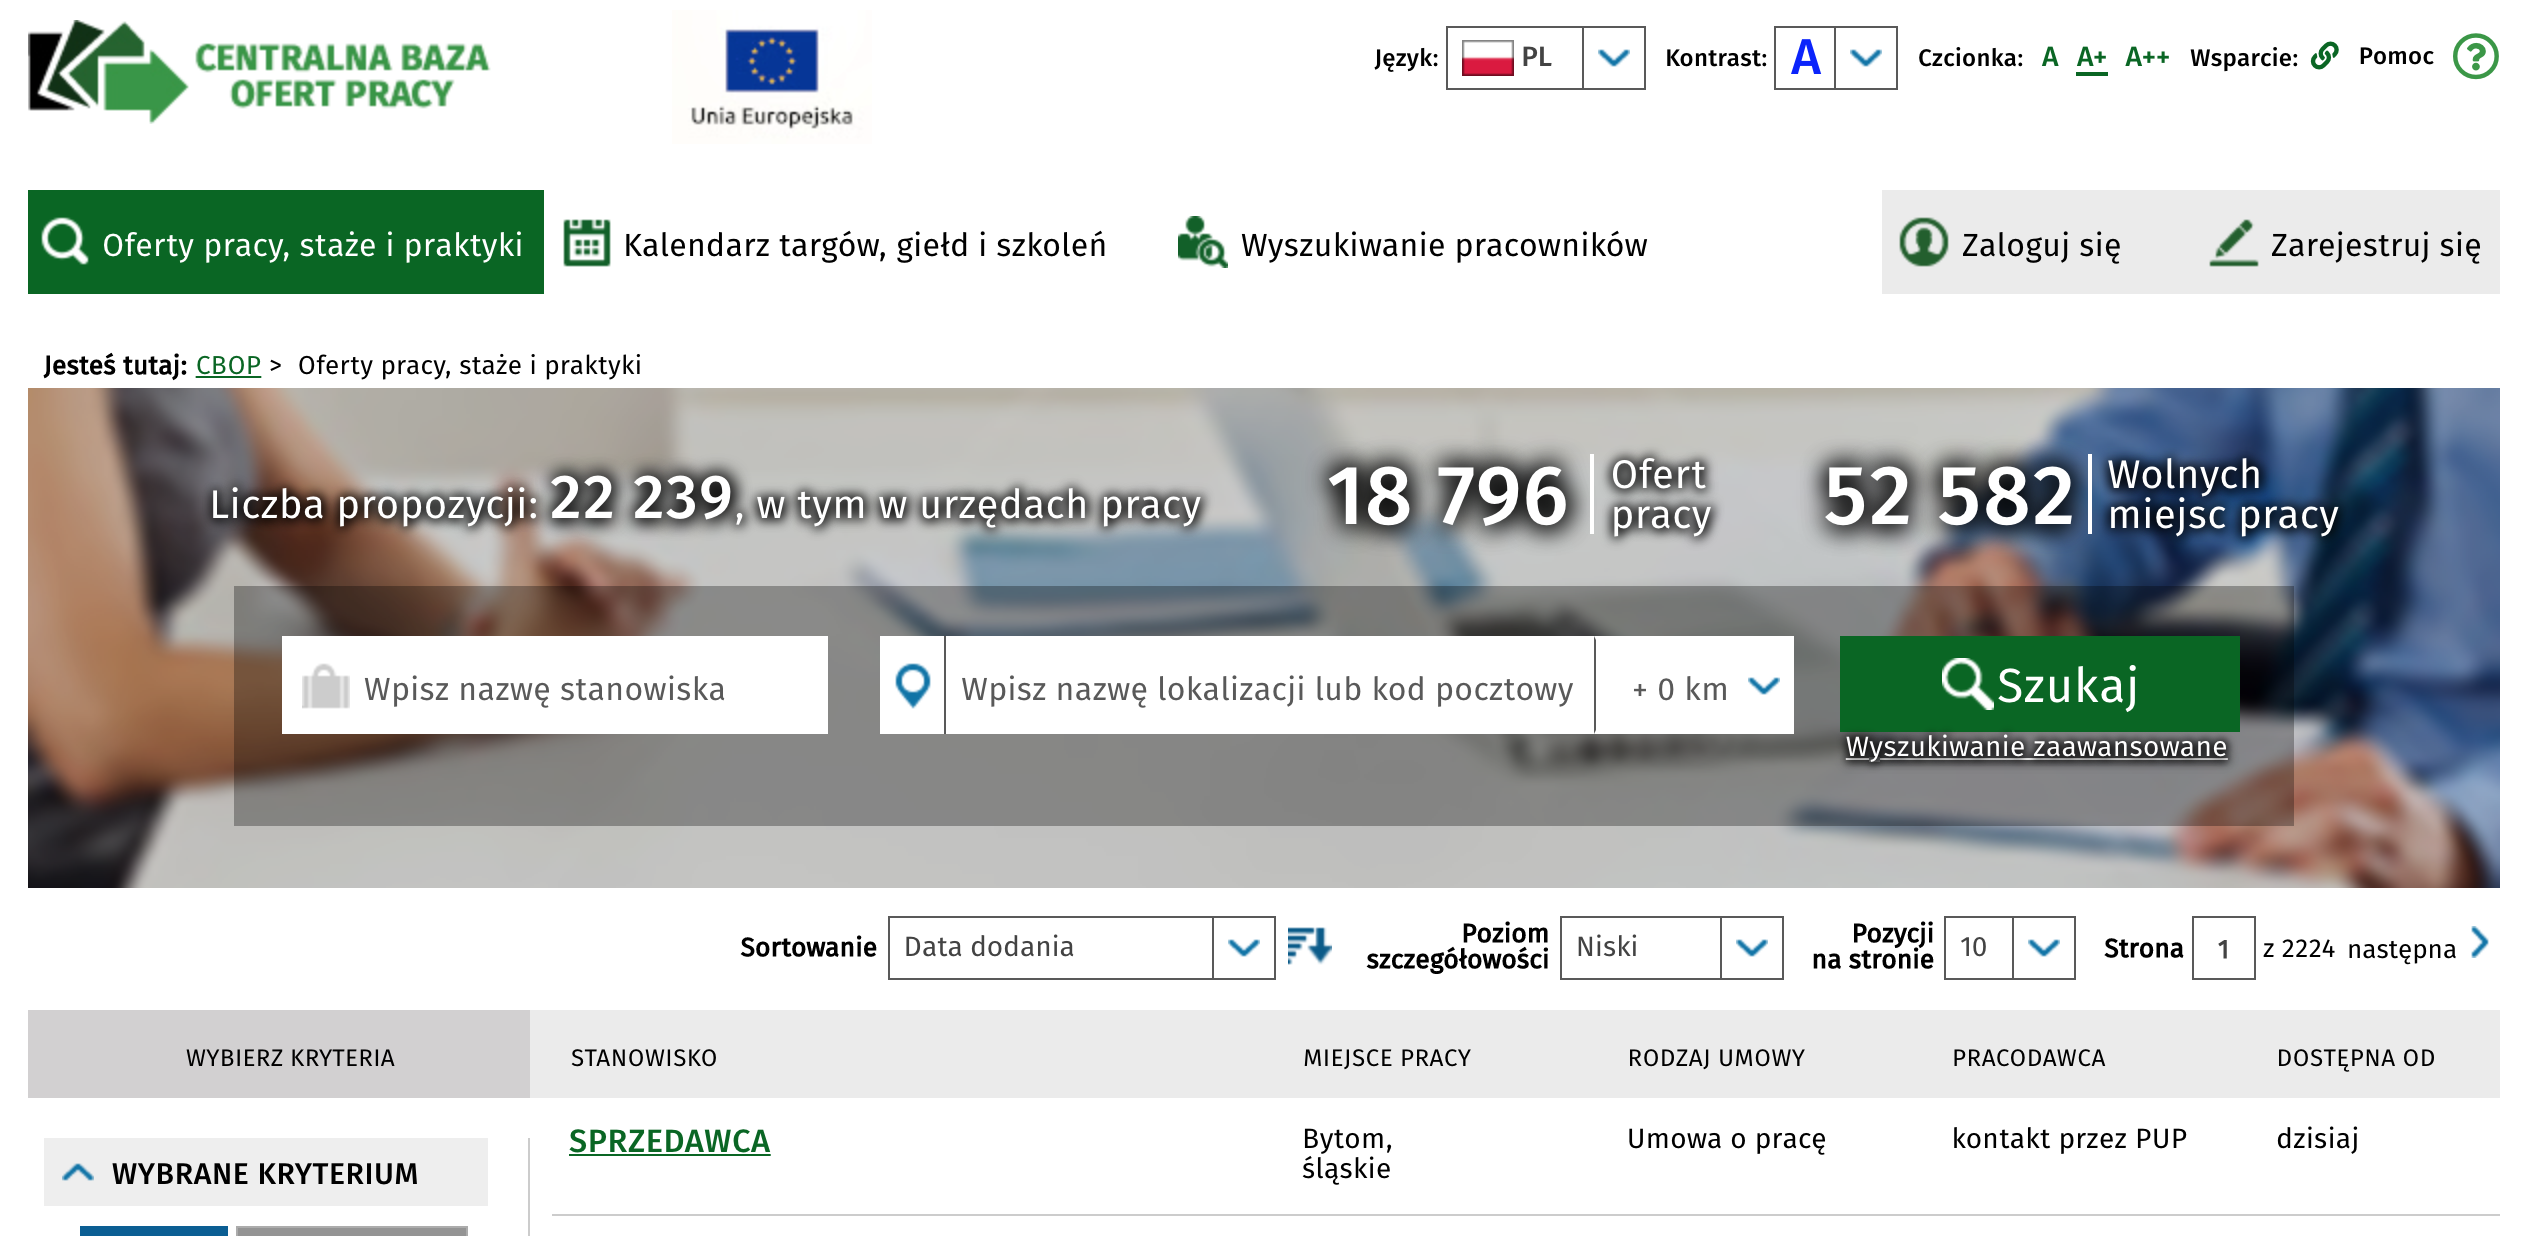
\includegraphics[width=\textwidth]{fig-2-definicje/cbop.png}
\end{figure}
\end{frame}

\begin{frame}{Przykład -- OtoDom}
\begin{figure}
    \centering
    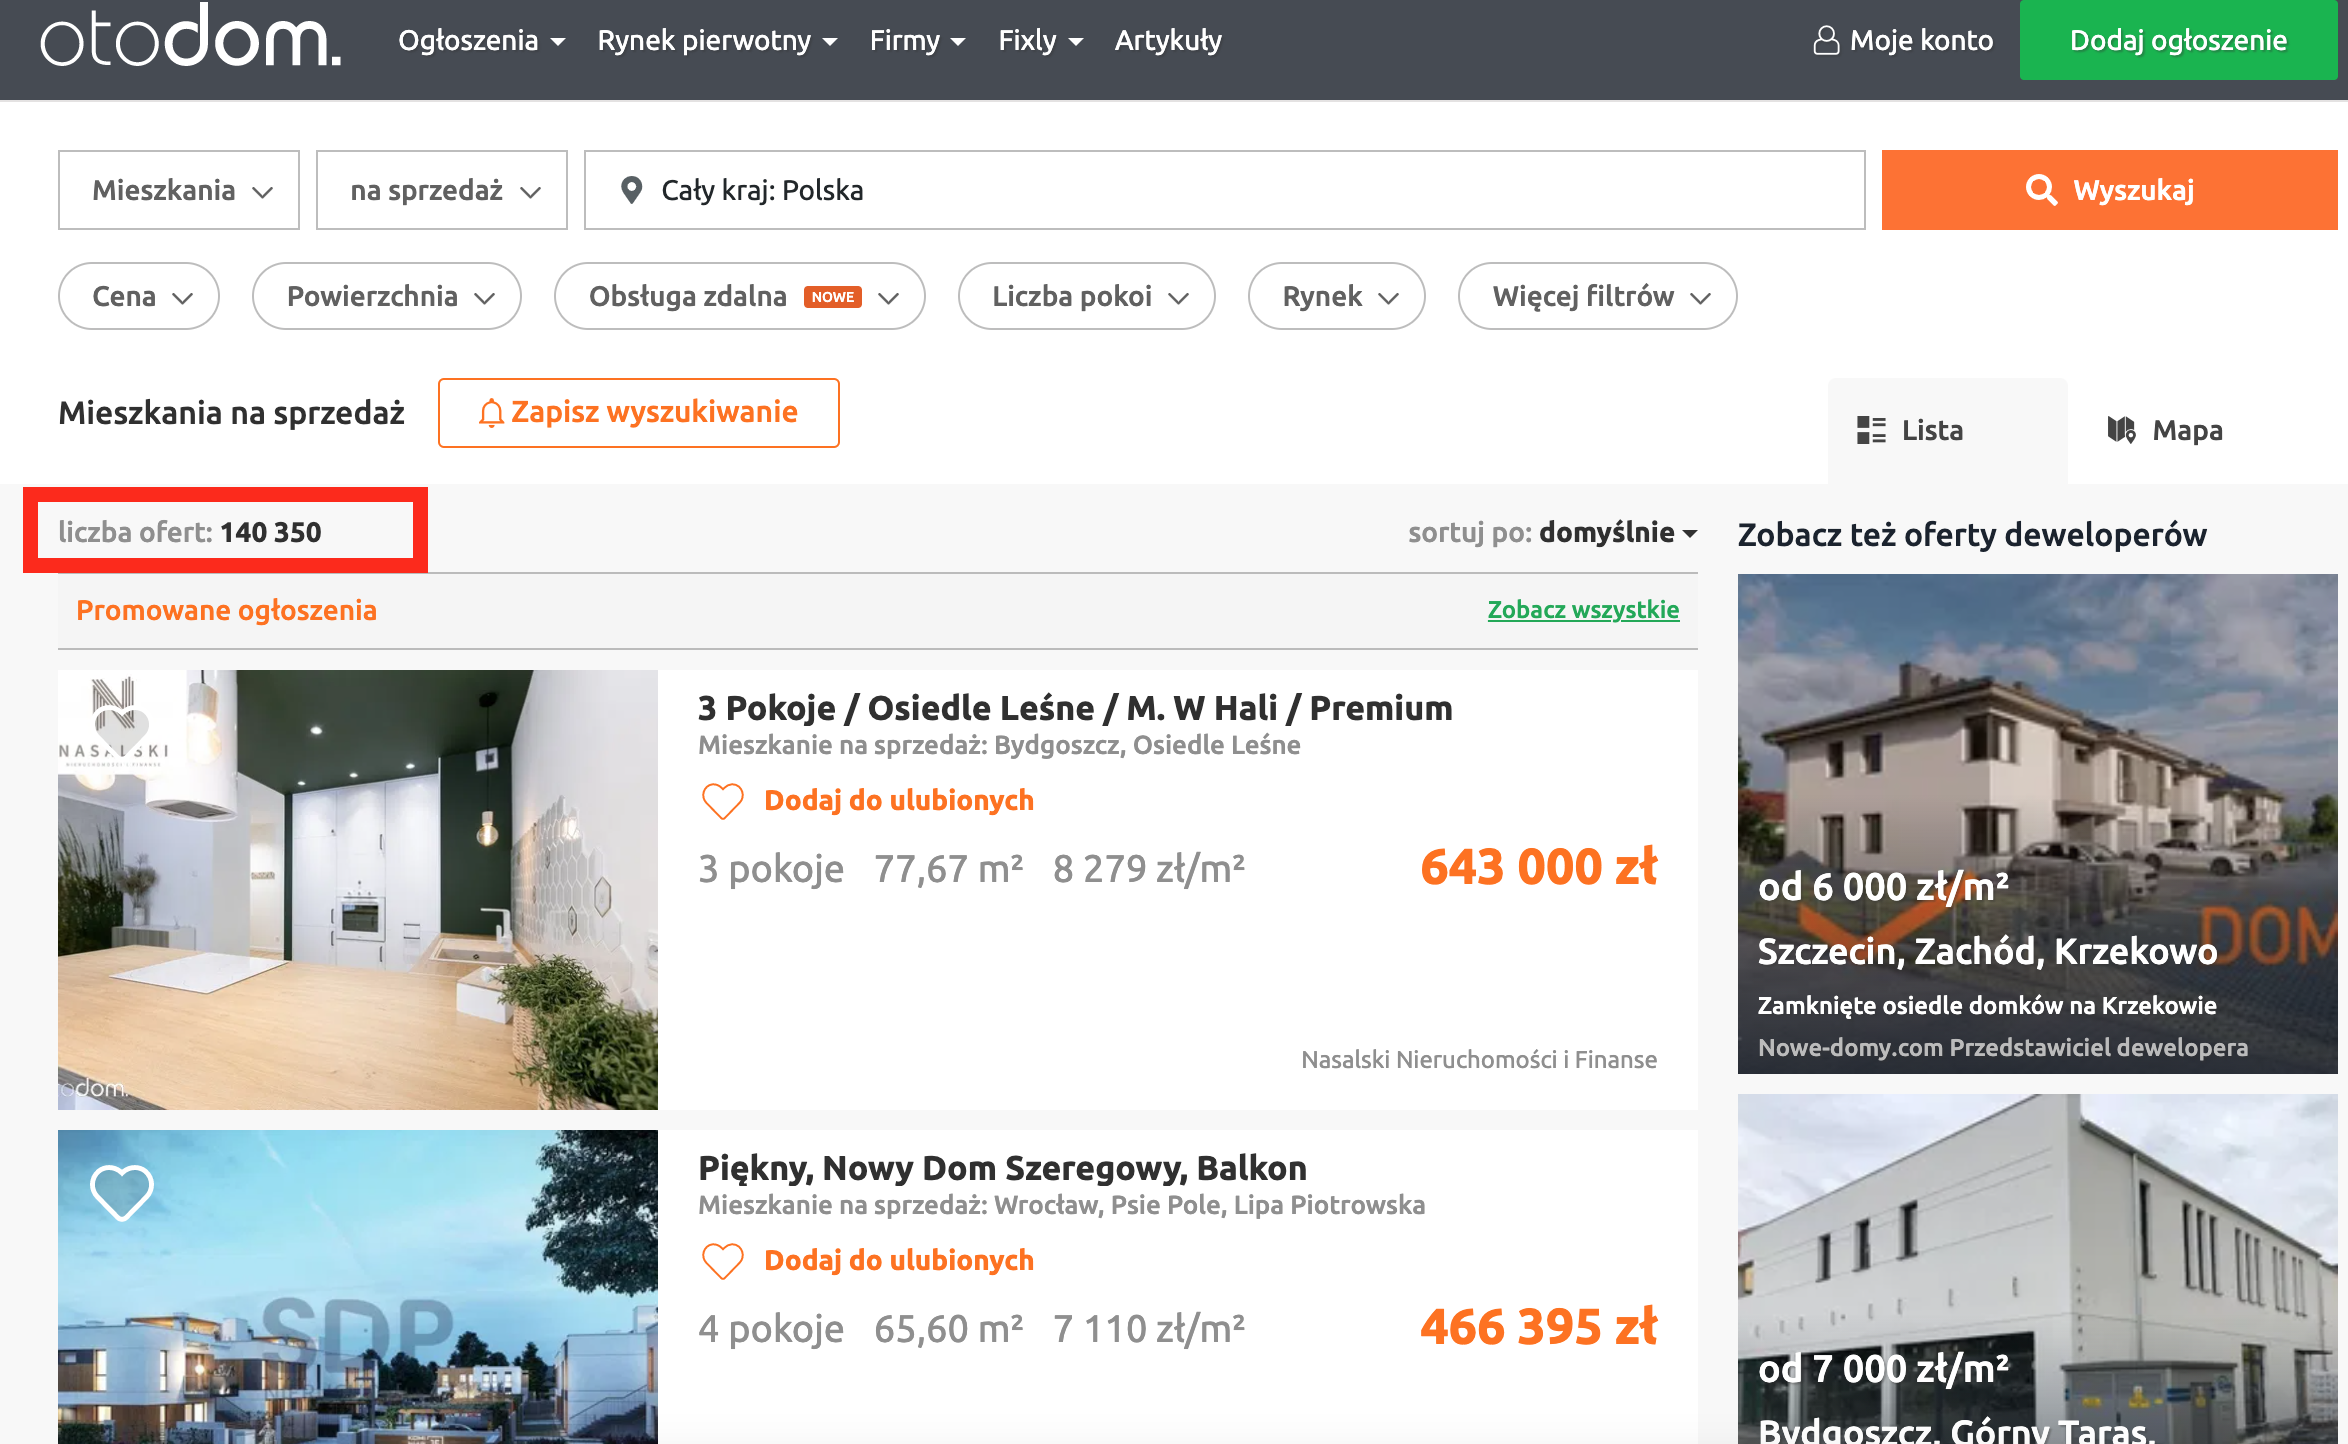
\includegraphics[width=\textwidth]{fig-2-definicje/otodom.png}

\end{figure}
\end{frame}

\begin{frame}{Przykład -- Kałużny, Beręsewicz i Filipowska (2018)}
\begin{figure}
    \centering
    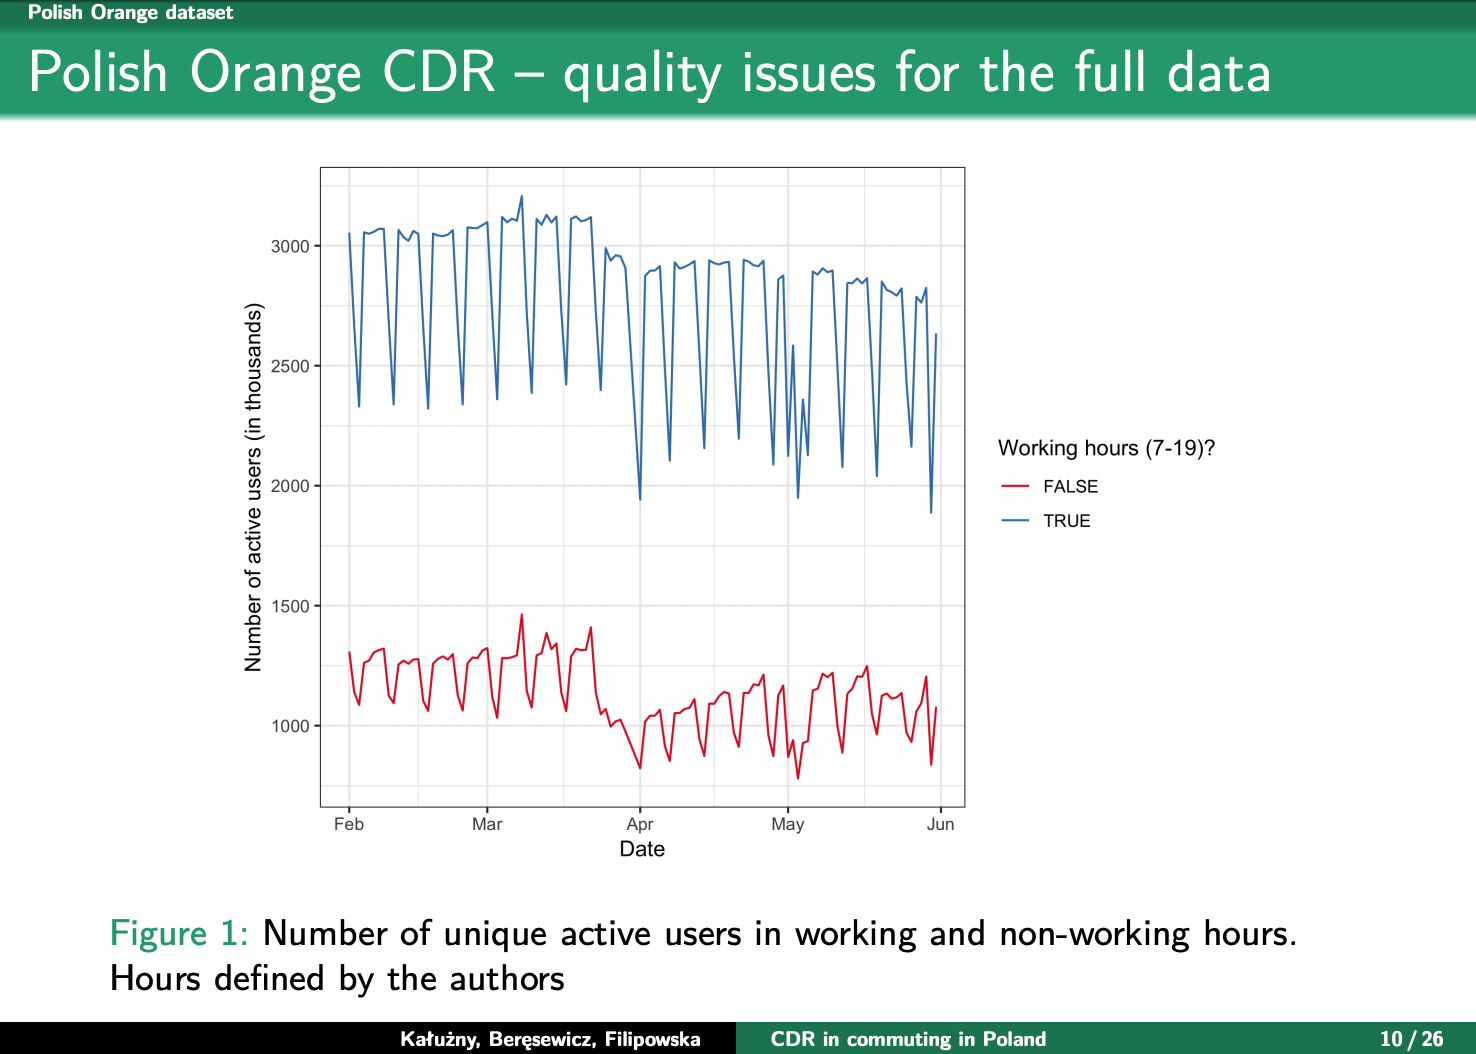
\includegraphics[width=\textwidth]{fig-2-definicje/cdr.png}
\end{figure}
\end{frame}

\begin{frame}{}
    \begin{center}
        \large
        
        Przejdźmy do precyzyjnych definicji reprezentatywności
        
    \end{center}
\end{frame}


\begin{frame}{Podstawowe oznaczenia}

\begin{itemize}
    \item $I_i = \{0, 1\}$ -- zmienna indykatorowa; określa czy dana jednostka $i$ była obserwowana w określonym zbiorze (np. ma dostęp do Internetu; ang. \textit{inclusion}).
    \item $R_i = \{0, 1\}$ -- zmienna indykatorowa; określa czy dana jednostka $i$ udzieliła odpowiedzi lub pseudo-odpowiedzi (np. umieściła wpis w Internecie; ang \textit{response}).
    \item $Y$ -- zmienna celu; cecha, którą badamy (np. poparcie dla danej partii)
    \item $y_i$ -- wartość, którą obserwujemy dla zmiennej celu (np. wskazanie nazwy partii),
    \item $\bX$ -- zmienne pomocnicze; cechy, które uważamy, że są związane z $Y$; $\bx_i$ -- wartości cech $\bX$, które obserwujemy w~zbiorze danych.
    \item $P(I_i=1)$ -- prawdopodobieństwo pokrycia.
    \item $P(R_i=1 | I_i=1) = \pi_i$ -- warunkowe prawdopodobieństwo pseudo-odpowiedzi (ang. \textit{propensity score}).
\end{itemize}
\end{frame}

\begin{frame}{Silna i słaba reprezentatywność}
    Schouten i in. (2009) zaproponował dwie definicje reprezentatywności w odniesieniu do odpowiedzi (ang. \textit{survey response}), które można ująć w kontekście losowego doboru do próby (braku autoselekcji), mianowicie:

\begin{itemize}
    \item Silna reprezentatywność
    \begin{equation}
  	\forall_i \; E(R_i) = \pi_i = P( R_i  = 1  \mid  I_i = 1) = \pi
	\label{def-strong} 
	\end{equation}
	\item Słaba reprezentatywność
	\begin{equation}
	    \bar{\pi}_h  = \frac{1}{N_h}\sum_{i=1}^{N_h} \pi_{ih} = \pi, \mbox{for $h=1,2,...,H$}
    \label{def-weak}
	\end{equation}
\end{itemize}

\small{Źródło: Schouten, B., Cobben, F., \& Bethlehem, J. (2009). Indicators for the representativeness of survey response. \textit{Survey Methodology}, 35(1), 101-113}

\end{frame}

\begin{frame}{Miniatura populacji}
    \begin{itemize}
        \item Próba jest reprezentatywna w odniesieniu do zmiennych pomocniczych ($\bx$) jeżeli rozkład cechy $\bX$ w próbie jest równy rozkładowi tej cechy w populacji przy założeniu losowego doboru próby
        
        \begin{equation}
            f_s(\bx_i, I_{i} = 1) = f_{\Omega}(\bx),    \label{definition-betlehem}
        \end{equation}
        
    \item Próba jest reprezentatywna w odniesieniu do zmiennych pomocniczych ($\bx$) jeżeli rozkład warunkowy cechy $\bX$ względem $\bw$ jest równy znanym wartościom globalnym (rozkładowi brzegowemu) tych cech w populacji generalnej.

    \begin{equation}
        f_s(\bx_i | w_i, I_{i} = 1) = f_{\Omega}(\bx),
    \label{definition-betlehem2}
    \end{equation}
    gdzie $w_i$ oznacza pewną wagę przypisaną danej jednostce $i$, którą może być zarówno odwrotność prawdopodobieństwa dostania się do próby $w_i = d_i = 1 / \pi_i$ czy wagi post-stratyfikowane czy kalibrowane.

    \end{itemize}
\end{frame}

\begin{frame}{Reprezentatywny model -- Pfeffermann (2011), Beręsewicz (2017)} 
    Na podstawie Pfeffermann(2011) można wskazać pojęcie reprezentatywnego modelu, które może być zdefiniowane następująco:

Model jest reprezentatywny, wtedy i tylko wtedy gdy rozkład warunkowy cechy $y$ pod warunkiem $\bx$ jest taki sam w próbie i populacji. To znaczy, $f_{s}(y_i | \bx_i) =  f_{\Omega}(y_i | \bx_i)$ tylko gdy

\begin{equation}
    Pr(R_i = 1 \mid \bx_i, y_i, I_i = 1)  = Pr(R_i = 1 \mid  \bx_i, I_i = 1).
\label{pfeffermann-equality}
\end{equation}

Pojęcie reprezentatywnego modelu możemy zapisać następująco:

\begin{equation}
    f_{s}(y_i | \bx_i) ={}  
f(y_i | \bx_i, I_i = 1, R_i=1) =  
\frac{Pr(R_i=1 \mid \bx_i, y_{i}, I_i=1)f_{\Omega}(y_i | \bx_i)}{Pr(R_i = 1 | \bx_i, I_i = 1)},
\label{def-pfefferman-modelling}
\end{equation}

gdzie $f_{s}(y_i | \bx_i)$ jest rozkładem warunkowym w próbie, $f_{\Omega}(y_i | \bx_i)$ jest rozkładem warunkowym w populacji, a pozostałe elementy zdefiniowane są jak poprzednio.
\end{frame}

\begin{frame}{Betlehem (1988, 2002, 2010)}
    Betlehem (1988, 2002, 2010) pokazał, że obciążenie estymatora średniej z próby zdefiniowanej jako
    
\begin{equation}
\bar{y}_{S}=\frac{1}{n_{S}} \sum_{i=1}^{N} R_{i} Y_{i},
\end{equation}

której wartość oczekiwana w przypadku próby internetowej dana jest

\begin{equation}
E\left(\bar{y}_{S}\right) \approx \bar{Y}_{I}^{*}=\frac{1}{N_{I} \bar{\pi}} \sum_{i=1}^{N} \pi_{k} I_{i} Y_{i},
\end{equation}

    może zostać zapisane jako
    
    \begin{equation}
        \boxed{B(\bar{y}_S) = \frac{Corr(\pi, Y) \sigma_\pi \sigma_Y}{\bar{\pi}},}
    \end{equation}
    
    gdzie $Corr(\pi, Y)$ to korelacja między $\pi$, a $Y$, $\sigma$ to odchylenie standardowe, a $\bar{\pi}$ to średnia arytmetyczna.
\end{frame}


\begin{frame}{Data Defect Index -- Xiao-Li MENG (2018)}
    \begin{figure}
        \centering
        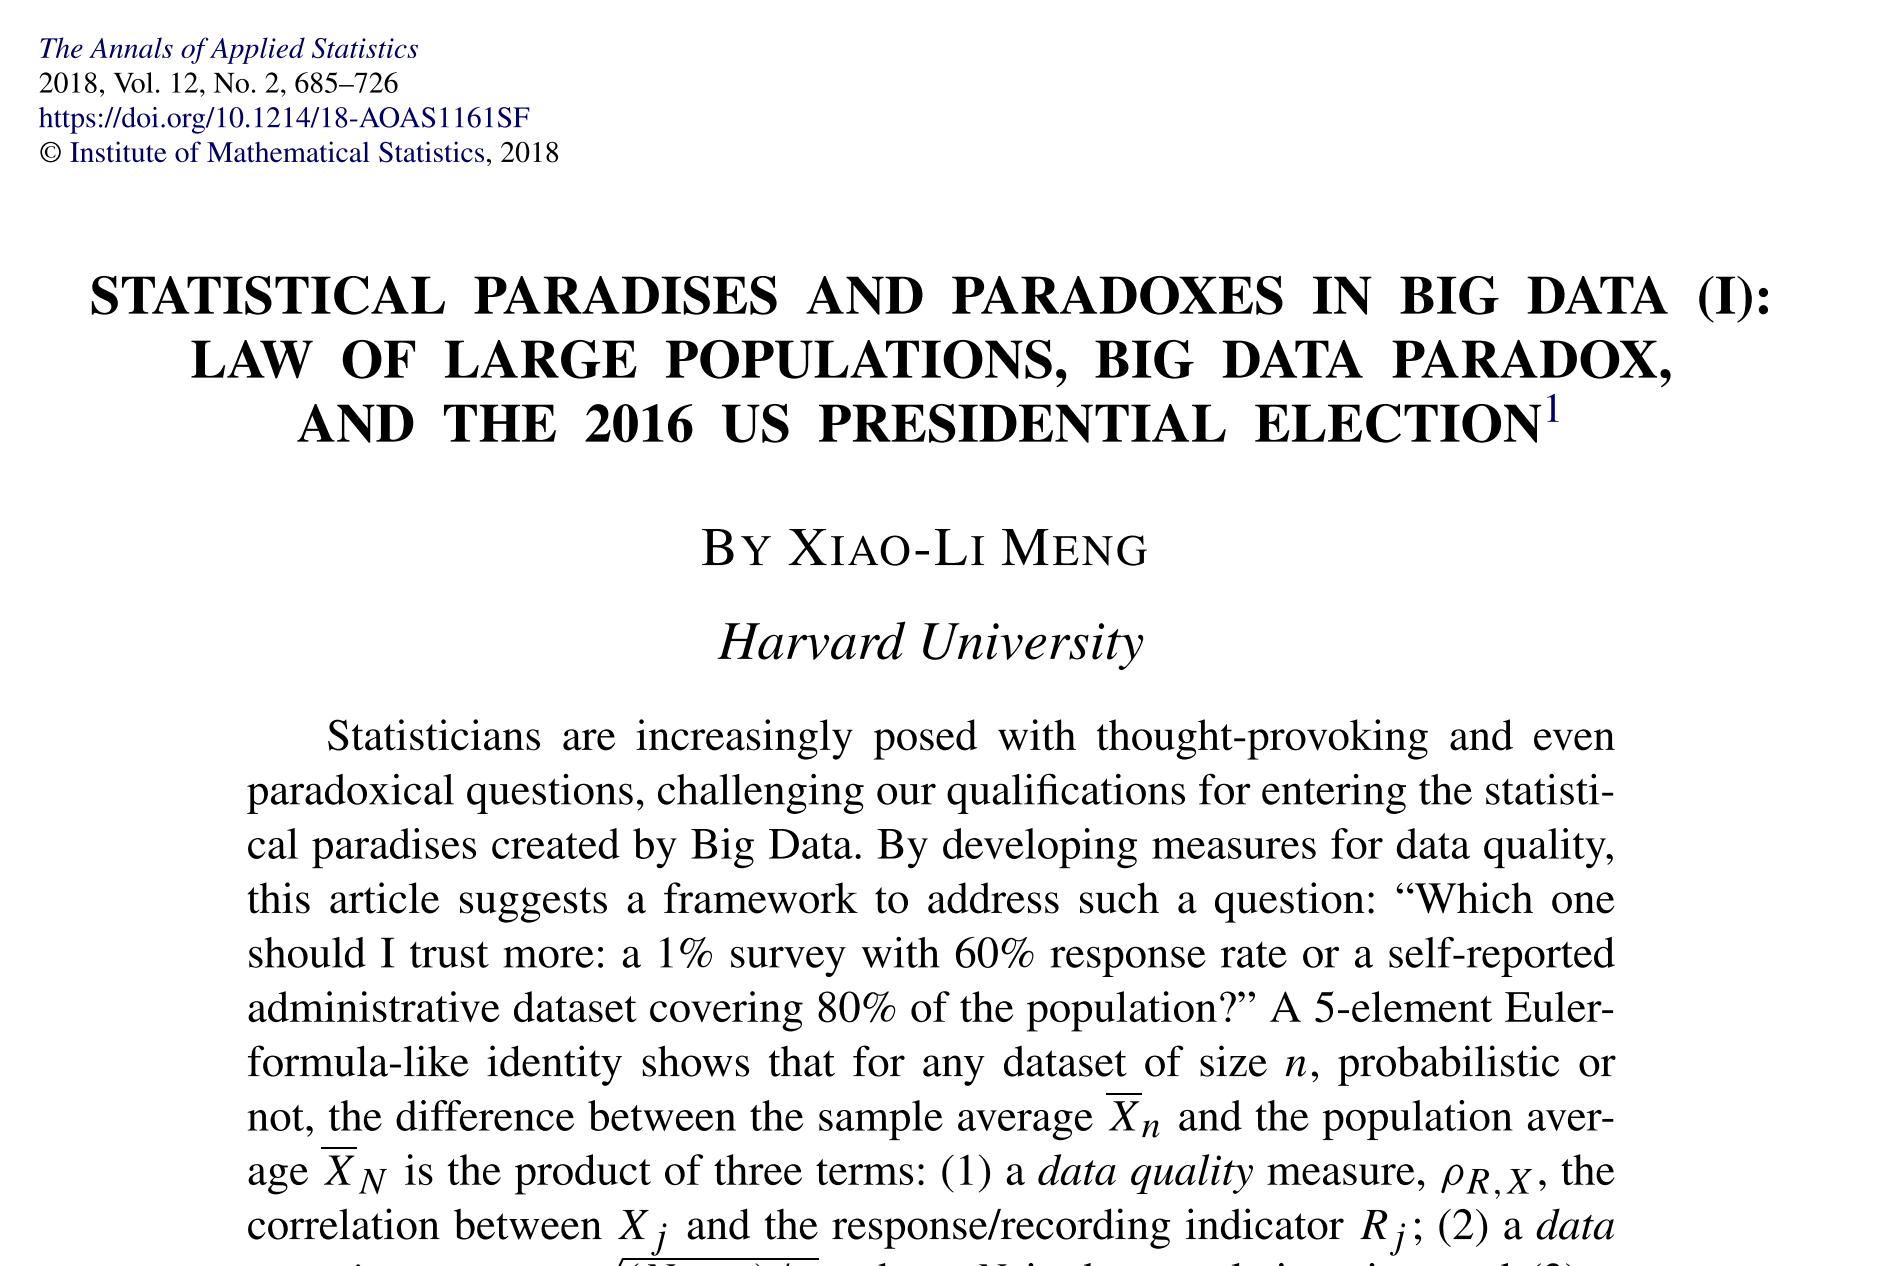
\includegraphics[width=\textwidth]{fig-2-definicje/meng.png}
    \end{figure}
\end{frame}

\begin{frame}{Data Defect Index -- Xiao-Li MENG (2018)}
 
\begin{equation}
\boxed{\overline{G}_{n}-\overline{G}_{N}=\underbrace{\rho_{R, G}}_{\text {Jakość danych}} \times \underbrace{\sqrt{\frac{1-f}{f}}}_{\text {Ilość danych}} \times \underbrace{\sigma_{G}}_{\text {Złożoność problemu}},}
\end{equation}

gdzie: 
\begin{itemize}
    \item $G_j = G(X_j)$ -- ogólna funkcja po zmiennych $X$, na przykład średnia arytmetyczna,
    \item $\overline{G}_{n}$ -- średnia z próby o liczebności $n$ ,
    \item $\overline{G}_{N}$ -- średnia w populacji o liczebności $N$,
    \item $\rho_{R, G} = Corr(R, G)$ -- korelacja między zmienną indykatorową $R$ a wartościami $G$ (\textbf{data defect correlation}),
    \item $\sqrt{(1-f)/f}$ -- $f$ oznacza odsetek w próbie tj. $f=n/N$,
    \item $\sigma_{G}$ -- odchylenie standardowe dla wartości funkcji $G$
\end{itemize}
Dowód: w artykule prof. Xiao-Li Menga.
\end{frame}

\begin{frame}{Prawo wielkich populacji (Meng, 2018)}
    W przypadku \textit{Big data} i występowaniu autoselekcji mierzonej $\rho_{R,G}$ następuje zmiana paradygmatu w ocenie błędów estymacji, tj.
    
    \vspace{0.5cm}
    
    przechodzimy z \textit{prawa wielkich liczb} i \textit{centralnego twierdzenia granicznego} według, którego
    
    
    \begin{equation}
        \boxed{\text{error} \propto \frac{\sigma}{\sqrt{n}},}
    \end{equation}
    
    \vspace{0.5cm}
    
    do relatywnego systematycznego błędu (\textit{prawa wielkich populacji}) według, którego
    
     \begin{equation}
        \boxed{\text{error} \propto \rho_{R,G} \cdot \sqrt{N}.}
    \end{equation}
\end{frame}

\begin{frame}{Przykład empiryczny -- Bradley i in. (2021, Nature)}
    \begin{itemize}
        \justifying
        \item Bradley i in. (2021) pokazali, że duże ankiety znacząco przeszacowały zaszczepienie COVID-19 w~USA:
        \begin{itemize}
            \item Delphi-Facebook ($\approx$250 tys. odpowiedzi/tydzień) -- przeszacowanie o~\textbf{17 p.p.}
            \item Census Household Pulse ($\approx$75 tys. co 2 tygodnie) -- przeszacowanie o~\textbf{14 p.p.}
            \item Axios-Ipsos ($\approx$1 tys./tydzień, dobrana próba panelowa) -- \textbf{trafne szacunki}
        \end{itemize}
        \item Jest to empiryczna ilustracja paradoksu Menga: zwiększenie wielkości próby zmniejsza przedział ufności, ale \textbf{powiększa efekt obciążenia} wynikającego z~autoselekcji.
    \end{itemize}

\small{Źródło: Bradley, V.C. i in. (2021). Unrepresentative big surveys significantly overestimated US vaccine uptake. \textit{Nature}, 600, 695--700.}
\end{frame}

\begin{frame}{Wybory w USA -- Clinton vs Trump}
    \begin{figure}
        \centering
        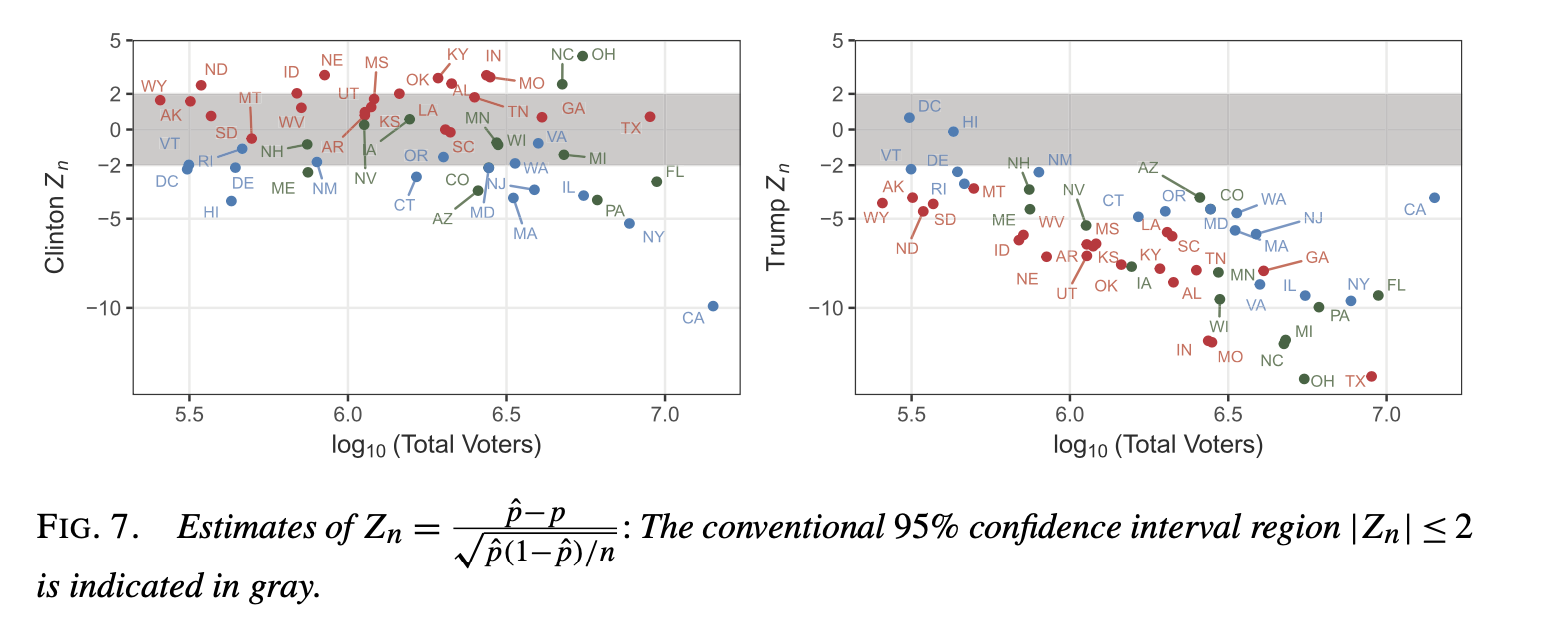
\includegraphics[width=\textwidth]{fig-2-definicje/meng-trump.png}
        \caption{Obliczone na podstawie próby n = 2,315,570 gdzie a N $\approx$ 136,700,730. Meng oszacował, że $\hat{\rho}=-0.005$. Źródło: Meng (2018)}
    \end{figure}
\end{frame}

\begin{frame}{DDI -- jak bardzo mylimy się w przypadku dużych prób?}

Celem przykładu będzie oszacowanie odsetka. Niech $G_n()$ będzie odsetkiem 1 dla zmiennej $Y = \{0, 1\}$, stosując standardowy test proporcji (przy założeniu rozkładu normalności) $Z_n$ będzie dany wzorem (za Mengiem)

\begin{equation}
    Z_n = \frac{\hat{p}-p}{\sqrt{\hat{p}(1-\hat{p})/n}} = 
    \frac{\sqrt{n}\sqrt{D_O}\rho_{R,G}}{
    \sqrt{1 - D_O\rho_{R,G}^2 - \sqrt{D_O}\rho_{R,G}
    \left( \sqrt{\frac{p}{1-p}} - \sqrt{\frac{1-p}{p}}\right)}
    },
\end{equation}

gdzie $D_O = (1-f)/f$. Załóżmy dla uproszczenia, że $p=0.5$ wtedy $Z_n$ redukuje się do

\begin{equation}
    Z_n = \sqrt{n}\sqrt{\frac{D_O\rho^2_{R,G}}{1-D_O\rho^2_{R,G}}}.
    \label{eq-meng-z}
\end{equation}

Dzięki \eqref{eq-meng-z} możemy porównać co by było w pytaniu: co wolimy 1\% próbę z 60\% realizacją czy 80\% próbę w postaci rejestru będącego wynikiem samo-rejestracji.
\end{frame}


\begin{frame}{DDI -- jak bardzo mylimy się w przypadku dużych prób?}

Załóżmy, że interesuje nas wnioskowanie o populacji Polski $N$=38 000 000.

\begin{table}
    \centering
    \caption{Porównanie $Z_n$ dla próby 80\% i 1\%}
    \label{tab:my_label}
    \begin{tabular}{ccc}
    \hline
    Parametr    &  80\% rejestr & 1\% próba\\
    \hline
    n     & 30,4 mln & 380 tys. \\
    $\rho_{R,G}$    & 0,005 & 0,001 \\
    $Z_n$ & 13.78 & 6.13 \\
    \hline
    \end{tabular}
\end{table}

Liczba 13 i 6 oznacza, że mylimy się o odpowiednio 13 i 6 odchyleń standardowych. \textbf{Oznacza to, mając próbę 30 mln mylimy się bardziej niż mając losową próbę.}

\vspace{0.5cm}

\textit{Uwaga}: przyjęliśmy tutaj, zgodnie z różnymi badaniami empirycznymi, że $\rho_{R,G}$ jest zwykle większe dla prób nielosowych (przykładowo Meng (2018) szacował  $\hat{\rho}_{R,G}=-0.005$ dla poparcia dla Trumpa).

\end{frame}


\begin{frame}{Zależność między X, Y, a R}
    \begin{figure}
        \centering  
        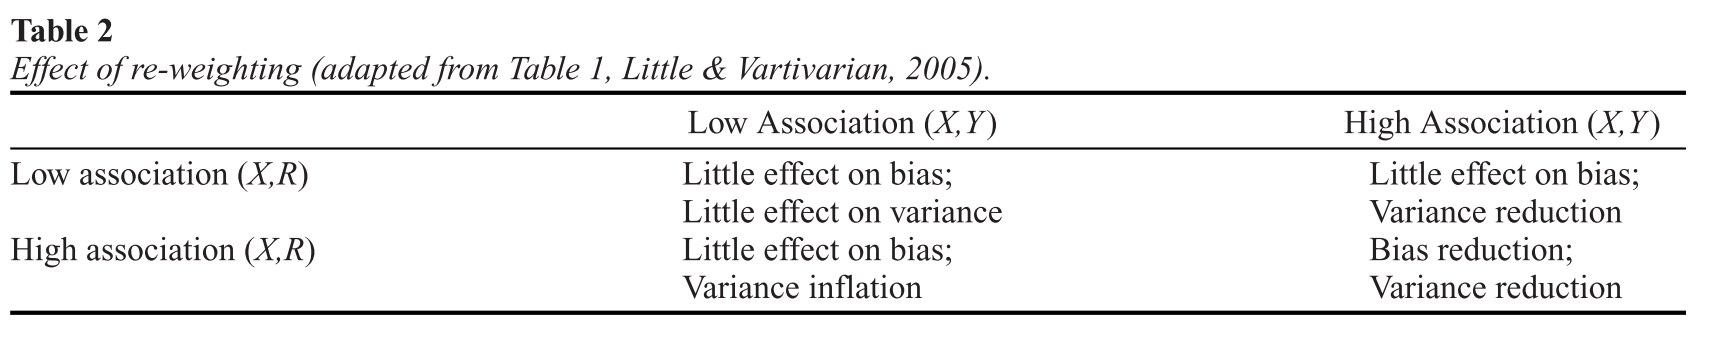
\includegraphics[width=\textwidth]{figs/zhang-relation.png}
        \caption{Zależność między cechami $\bX$, $Y$ oraz $R$. }
    \end{figure}
    
Gdzie: $\bX$ -- zmienne pomocnicze, $Y$ zmienna celu oraz $R = \{0,1\}$.

\vspace{0.5cm}

\small{Źródło: Zhang, L. C., Thomsen, I. B., \& Kleven, Ø. (2013). On the Use of Auxiliary and Paradata for Dealing With Non‐sampling Errors in Household Surveys. International Statistical Review, 81(2), 270-288.}

\end{frame}

\begin{frame}{Jaki jest z tego wniosek?}
    \begin{itemize}
        \item Redukcja obciążenia występuje tylko wtedy kiedy $\bX$ i $Y$ są ze sobą silnie skorelowane ($|Corr(Y,\bX)| > 0$)
        \item Redukcja obciążenia występuje tylko wtedy kiedy $\bX$ i $R$ są ze sobą silnie skorelowane  ($|Corr(R,\bX)| > 0$)
        \item Korelacja miedzy $Y$ i $R$ jest bliska zeru gdy  ($|Corr(Y,R| \bX)| \approx 0$)
        \item Konieczne jest posiadanie informacji o $X$, a najlepiej gdybyśmy dysponowali zmienną $X_k$, która jest tzw. \textit{proxy variable} -- zbliżona ale nie ta sama definicja  (np. cena ofertowa vs cena transakcyjna).
    \end{itemize}
\end{frame}

\begin{frame}{Inne miary reprezentatywności}

\begin{itemize}
    \justifying
    \item \textbf{R-indicator} (Schouten, Cobben, Bethlehem, 2009) -- mierzy zmienność prawdopodobieństw odpowiedzi $\pi_i$:
    \begin{equation}
        R = 1 - 2 S(\hat{\pi}_i),
    \end{equation}
    gdzie $S(\hat{\pi}_i)$ to odchylenie standardowe oszacowanych prawdopodobieństw odpowiedzi. $R = 1$ oznacza pełną reprezentatywność (stałe $\pi_i$), a $R$ bliskie 0 oznacza silną niereprezentatywność.

    \item \textbf{Metryki odległości} (Shlomo i Kim, 2025) -- porównanie rozkładów zmiennych pomocniczych w próbie i populacji z wykorzystaniem miar odległości (np. Hellinger, $\chi^2$).

    \item \textbf{Standaryzowane różnice średnich} (SMD) -- miara stosowana w kontekście propensity score weighting, pozwalająca ocenić balans zmiennych pomocniczych.
\end{itemize}

\vspace{0.3cm}
\small{Źródła: Schouten i in. (2009). \textit{Survey Methodology}, 35(1); Shlomo, N. i Kim, M.S. (2025). \textit{Survey Methodology}, 51(2).}
\end{frame}

\begin{frame}[fragile]{Data Defect Index -- przykład w R}

\begin{columns}
\begin{column}{0.5\textwidth}
\small
\begin{verbatim}
library(ddi)
data(g2016)

# ddc dla calego USA
ddc(
  mu    = 62984824/136639786,
  muhat = 12284/35829,
  N     = 136639786,
  n     = 35829
)
# [1] -0.003837163

# ddi = rho^2
(-0.003837)^2
# [1] 1.47e-05
\end{verbatim}
\end{column}

\begin{column}{0.5\textwidth}
\small
\begin{itemize}
    \item $\hat{\rho} \approx -0.004$ -- wyborcy Trumpa niedoreprezentowani w~CCES
    \item Mimo małej korelacji, przy $N \approx 137$ mln, błąd kumuluje się
    \item DDI jest \textbf{model-free}: nie wymaga estymacji propensity score, wystarczy znać $\mu$, $\hat{\mu}$, $N$, $n$
    \item Pakiet R: \texttt{ddi} (Kuriwaki)
\end{itemize}
\end{column}
\end{columns}
\end{frame}

\begin{frame}{Krótkie podsumowanie dotychczasowej wiedzy}
    \begin{table}
        \centering
        \caption{Próby losowe, a nielosowe}
        \begin{tabular}{lll}
        \hline
        \textbf{Czynnik}     &  \textbf{Próba losowa} & \textbf{Próba nielosowa}\\
        \hline
        Dobór     &  Schemat losowania & Auto-selekcja \\
        Pokrycie     &  Zwykle dobre & Pewne grupy są wykluczone \\
        Obciążenie & Zwykle mniejsze & duże, lub bardzo duże \\
        Wariancja & Zwykle większa & Mała, lub bardzo mała \\
        Koszt & Duży lub bardzo duży & Zwykle nieduży \\
        \hline
        \end{tabular}

    \end{table}
\end{frame}


\begin{frame}{Zadanie 1: Oblicz Data Defect Correlation (15 min)}

Ankieta internetowa szacowała frekwencję wyborczą w 6 województwach. Poniżej oficjalne wyniki (PKW) i szacunki z ankiety. Przyjmij $\sigma_G = 0.49$.

\begin{table}
    \centering
    \small
    \begin{tabular}{lrrcc}
    \hline
    Województwo & $N$ & $n$ & $\mu$ (PKW) & $\hat{\mu}$ (ankieta) \\
    \hline
    mazowieckie   & 4 200 000 & 12 000 & 0.68 & 0.79 \\
    śląskie       & 3 500 000 &  8 500 & 0.58 & 0.71 \\
    wielkopolskie & 2 700 000 &  5 200 & 0.62 & 0.73 \\
    małopolskie   & 2 600 000 &  6 800 & 0.65 & 0.74 \\
    dolnośląskie  & 2 300 000 &  4 900 & 0.60 & 0.72 \\
    podkarpackie  & 1 600 000 &  1 200 & 0.55 & 0.63 \\
    \hline
    \end{tabular}
\end{table}

\begin{enumerate}
    \item Oblicz błąd estymacji $\hat{\mu} - \mu$ dla każdego województwa.
    \item Oblicz $\rho_{R,G} = \frac{\hat{\mu} - \mu}{\sigma_G \cdot \sqrt{(1-f)/f}}$, gdzie $f = n/N$.
    \item Czy ankieta zawyża czy zaniża frekwencję? Dlaczego?
    \item W którym województwie autoselekcja jest najsilniejsza?
\end{enumerate}

\end{frame}


\begin{frame}{Zadanie 2: 1\% próba losowa vs.\ 80\% rejestr (15 min)}

Cel: oszacować odsetek osób popierających partię X w~Polsce ($N = 30$ mln). Dysponujemy dwoma źródłami. Przyjmij $p = 0.5$.

\begin{table}
    \centering
    \begin{tabular}{lcc}
    \hline
    Parametr & Próba losowa & Rejestr \\
    \hline
    $n$           & 300 000 (1\%) & 24 000 000 (80\%) \\
    $\rho_{R,G}$  & 0.001         & 0.005 \\
    \hline
    \end{tabular}
\end{table}

Wzór na statystykę testową (przy $p = 0.5$):

\begin{equation*}
    Z_n = \sqrt{n} \cdot \sqrt{\frac{D_0 \cdot \rho_{R,G}^2}{1 - D_0 \cdot \rho_{R,G}^2}} \approx \sqrt{N - n} \cdot \rho_{R,G}, \quad \text{gdzie } D_0 = \frac{1-f}{f}.
\end{equation*}

\textbf{Wskazówka:} $\sqrt{n} \cdot \sqrt{D_0} = \sqrt{n \cdot \frac{N-n}{n}} = \sqrt{N-n}$, więc $Z_n$ zależy od wielkości \textbf{populacji}, nie próby.

\begin{enumerate}
\small
    \item Oblicz $f$, $N - n$ i $Z_n$ dla obu źródeł.
    \item Które źródło daje większy błąd (w odchyleniach standardowych)?
    \item O ile musielibyśmy zmniejszyć $\rho_{R,G}$ w rejestrze, żeby $Z_n < 2$?
    \item Jaki wniosek płynie z tego porównania?
\end{enumerate}

\end{frame}


% % \section{Badania symulacyjne}


% % \begin{frame}{Badania symulacyjne}
 
% % W statystyce i ekonometrii, celem badań symulacyjnych jest zweryfikowanie
% %     \begin{itemize}
% %         \item poprawności implementacji konkretnych podejść (np. czy dany program poprawie oszacowuje konkretne parametry),
% %         \item porównaniu różnych metod (np. czy faktycznie proponowana metoda działa lepiej niż inne),
% %         \item analizę wrażliwości (np. jak bardzo odporna jest dana metoda na złamanie założeń).
% %     \end{itemize}
    
% %     Na dzisiejszych zajęciach, które będą przydatne z punktu projektu, będę chciał pokazać Państwu jak można prowadzić takie badania symulacyjne na podstawie wybranych publikacji naukowych.
% % \end{frame}

% % \begin{frame}{Kim i Wang (2018)}
% %     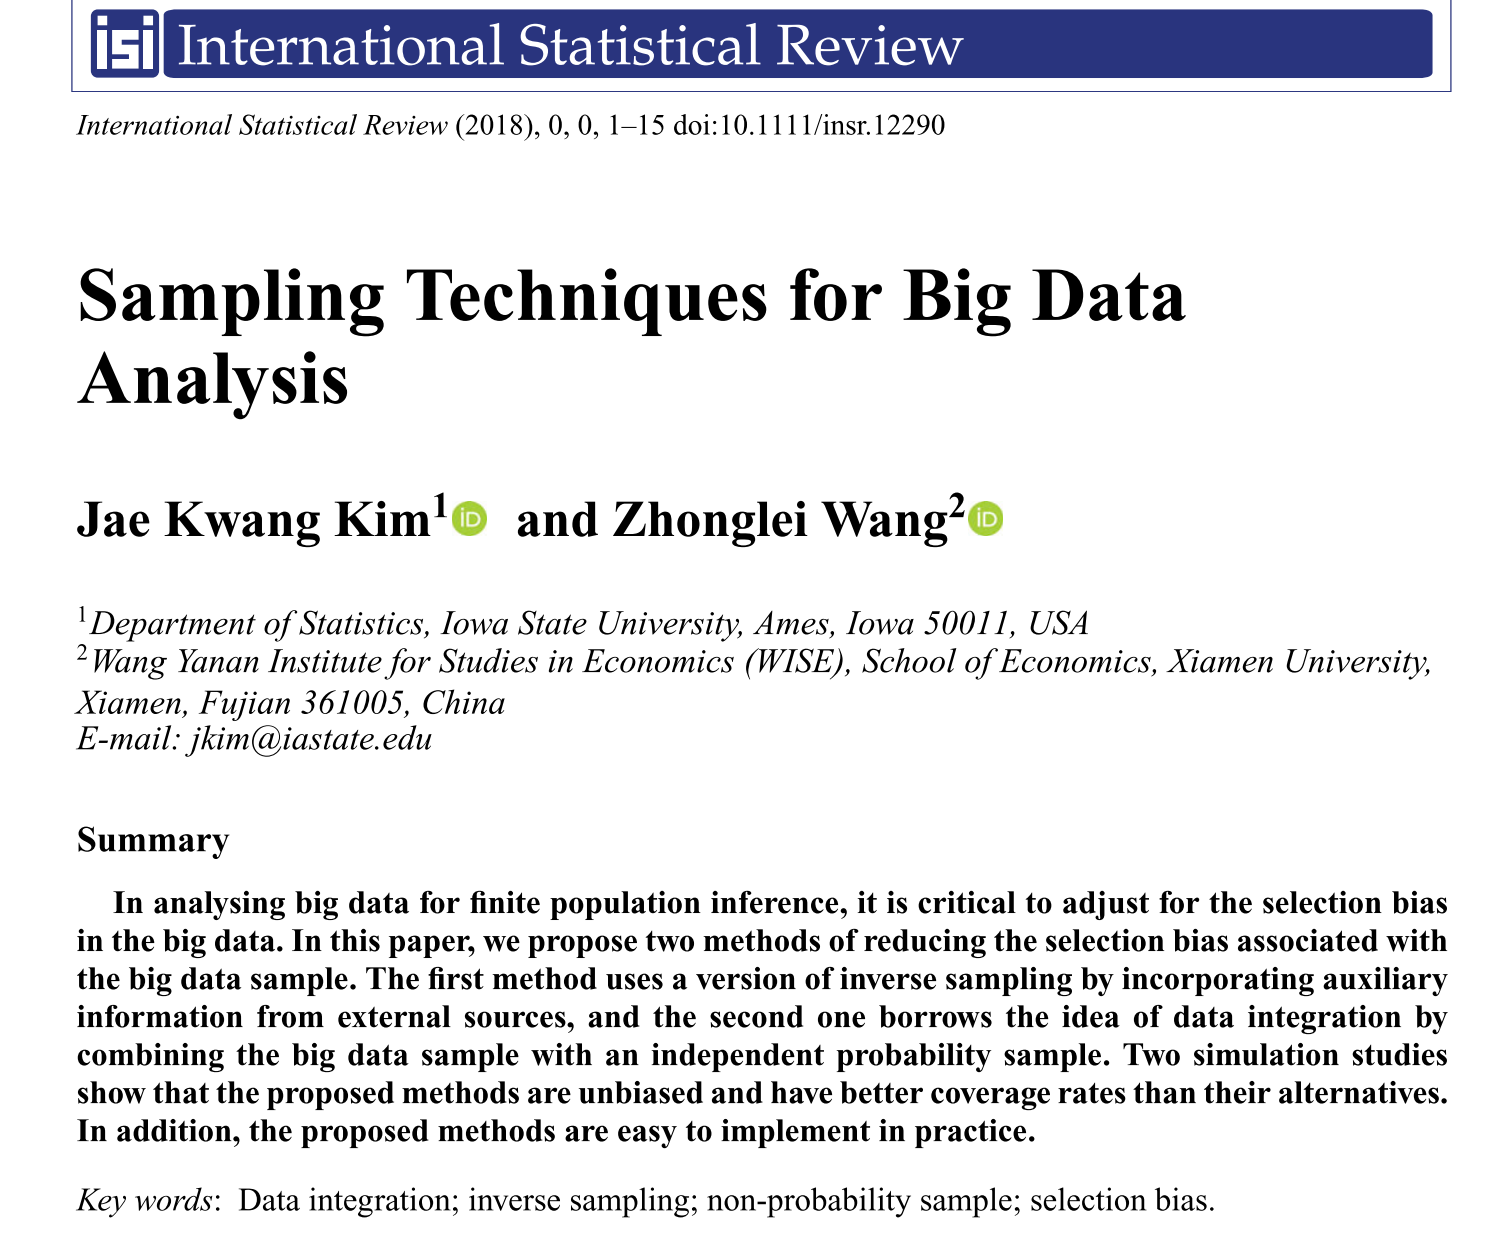
\includegraphics[width=0.9\textwidth]{fig-3-sims/sim-2.png}
% % \end{frame}

% % \begin{frame}{Kim i Wang (2018) -- badanie symulacyjne -- założenia}
% %     \begin{itemize}
% %         \item Celem badania było zweryfikowanie skuteczności metod estymacji w przypadku prób nielosowych.
% %         \item Metody zaproponowane przez Kim'a i Wang'a (2018) zakładają istnienie dwóch prób: losowej (o liczebności 500 lub 1 000) oraz nielosowej.
% %         \item Próba losowa została wylosowania stosując losowanie proste bez zwracania.
% %         \item Przynależność do próby losowej wylosowano zgodnie z rozkładem Bernulliego ($\delta_i \sim Bern(p_i)$)
% %         \item Wielkość populacji ($N$) ustalono na 1 000 000.
% %         \item Zmienne objaśniające ($X_1$ i $X_2$) oraz błąd losowy ($\epsilon$) były wygenerowane zgodnie z następującym układem
% %         \begin{equation}
% %             \begin{aligned}
% %                 X_1 & \sim N(1,1), \\
% %                 X_2 & \sim Exp(1), \\ 
% %                 \epsilon & \sim N(0,1).
% %             \end{aligned}
% %         \end{equation}
% %     \end{itemize}    
% % \end{frame}

% % \begin{frame}{Kim i Wang (2018) -- badanie symulacyjne -- założenia}
% % \begin{itemize}
% %     \item Następnie wygenerowano dwie zmienne celu $Y_1$ i $Y_2$ według następujących modeli
    
% %     \begin{equation}
% %         \begin{aligned}
% %             Y_1 & = 1 + X_1 + X_2 + \epsilon, \\
% %             Y_2 & = 0.5(X_1-0.5)^2 + X_2 + \epsilon.
% %         \end{aligned}
% %     \end{equation}
% %     \item Identyfikator $\delta_i$ wylosowano z rozkładu Bernoullego zgodnie z prawdopodobieństwem $p_i$ danym dwoma wzorami:
% %         \begin{equation}
% %             \begin{aligned}
% %                 \text{logit}(p_1) & = X_2 \quad, \text{czyli} \frac{\exp(X_2)}{1 + \exp(X_2)}, \\
% %                 \text{logit}(p_2) & = -0.5 + 0.5(X_2-2)^2 \quad, \text{czyli} \frac{\exp(-0.5 + 0.5(X_2-2)^2)}{1 + \exp(-0.5 + 0.5(X_2-2)^2)}.
% %             \end{aligned}
% %         \end{equation}
% % \end{itemize}
% % \end{frame}

% % \begin{frame}{}
% %     \begin{center}
% %         \Large
        
% %         Przejdźmy do R. 
        
% %     \end{center}
% % \end{frame}
% % \begin{frame}{Betlehem (2010)}
% %     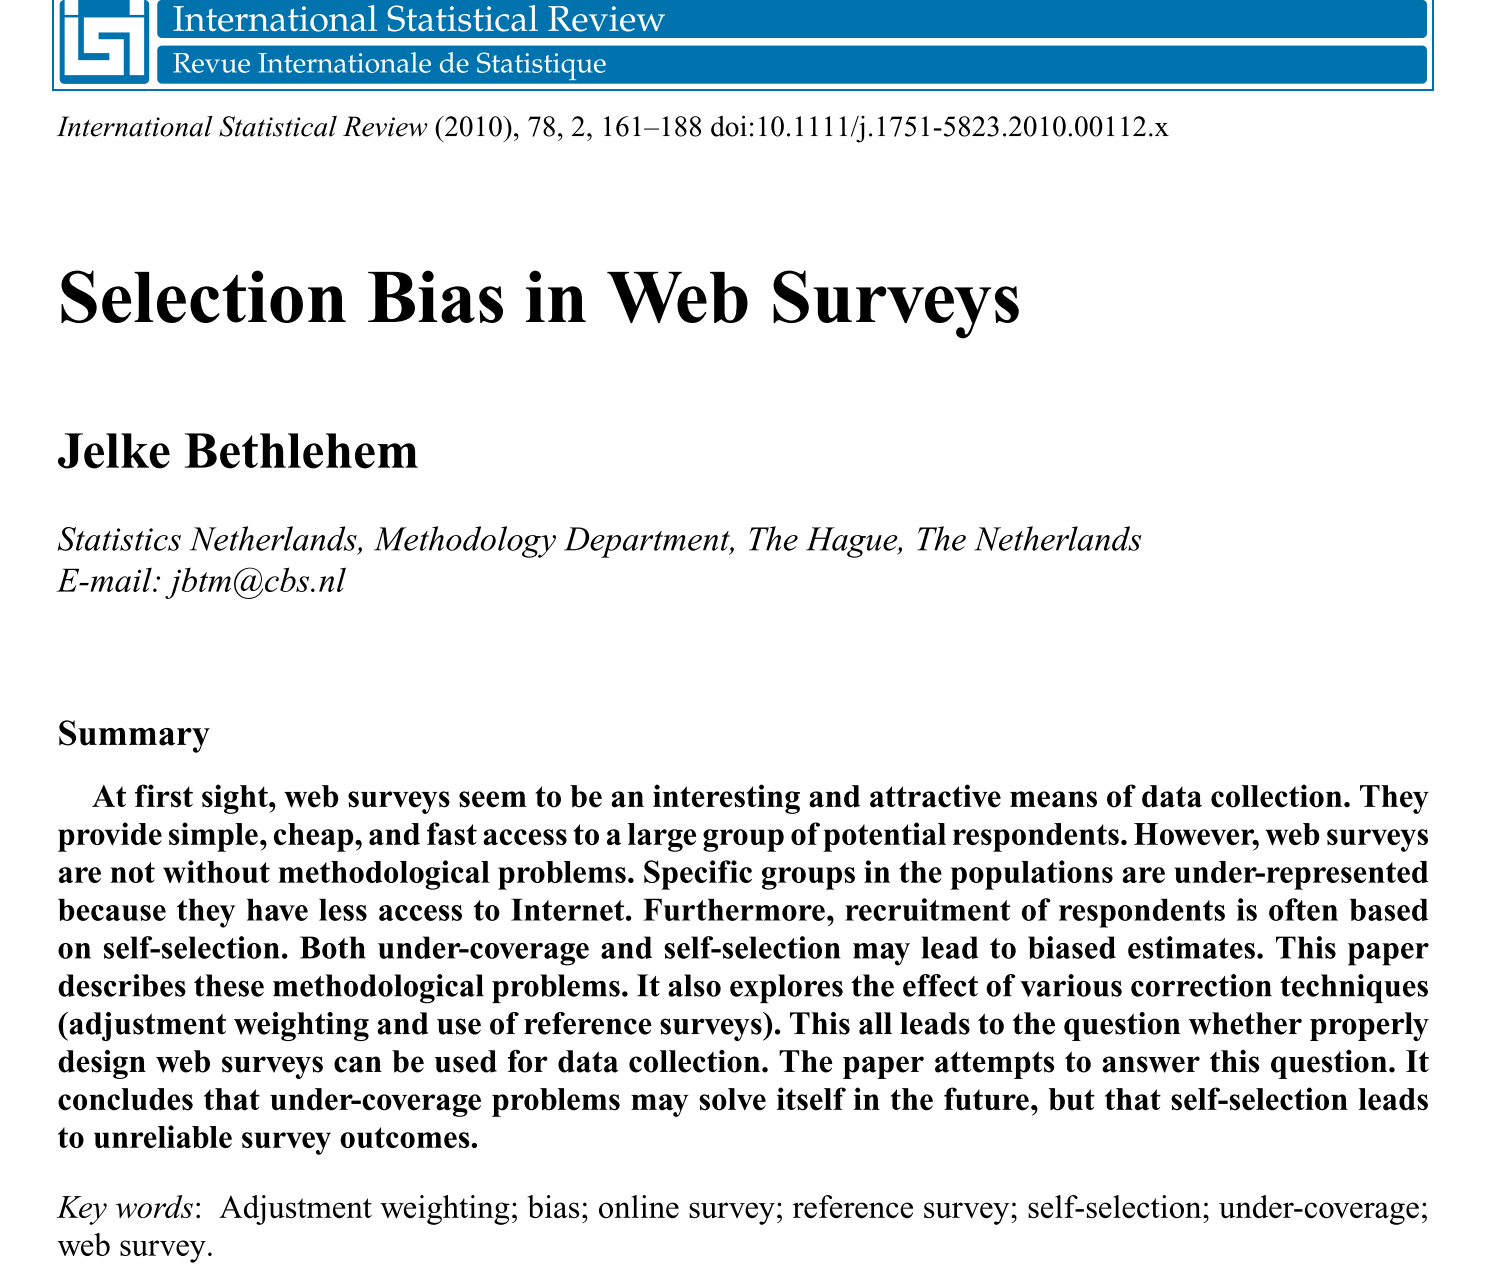
\includegraphics[width=0.9\textwidth]{fig-3-sims/sim-1.png}
% % \end{frame}


% % \begin{frame}{Betlehem (2010) -- badanie symulacyjne -- założenia}
% %     \begin{itemize}
% %         \item Celem badania było zweryfikowanie skuteczności metod estymacji w zależności od różnych scenariuszy powstawania 
% %         \item Badanie dotyczyło poparcia dla dwóch fikcyjnych partii politycznych: the National Elderly Party (NEP) oraz the New Internet Party (NIP).
% %         \item Założono następujące zależności między zmiennymi, które zostały odpowiednio utworzone na potrzeby tego badania.
% %         \begin{figure}
% %             \centering
% %             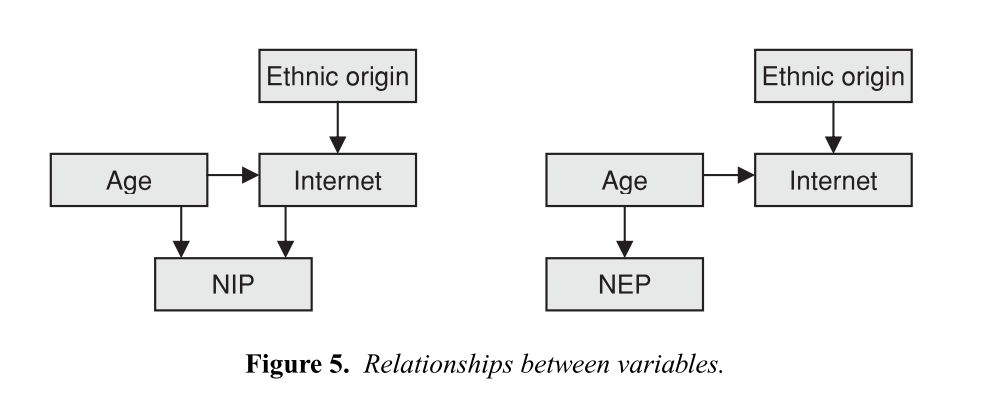
\includegraphics[width=0.6\textwidth]{fig-3-sims/sim-1-zal.png}
% %         \end{figure}
% %         \item W badaniu utworzono pseudo-populację o wielkości 30 tys., z której dokonywano losowania prostego: z całej populacji i tylko z populacji internetowej (obie po 2 000 jednostek)
% %     \end{itemize}
% % \end{frame}

% % \begin{frame}{Betlehem (2010) -- badanie symulacyjne -- generowanie (1)}

% % W jaki sposób utworzono zmienne (jest to metoda nieparametryczna)

% % \begin{itemize}
% %     \item Wiek w grupach (age): młodzi (40\%), średni (35\%), starsi (25\%),
% %     \item Pochodzenie (ethnic origin): rodzimi mieszkańcy (85\%), obcokrajowcy (15\%),
% %     \item Posiadanie dostępu do Internetu (Tak/ Nie). założono, że zależy od pochodzenia (ethnic) i wieku (age):
% %         \begin{table}
% %             \centering
% %             \begin{tabular}{llrr}
% %             \hline
% %              Przekroje   & Internet &  Tak & Nie\\
% %             \hline 
% %               Rodzimi   & Młodzi   &  90\% &  10\% \\
% %                         &  Średni  &  70\% &  30\% \\
% %                         &  Starsi  &  50\% & 50\% \\
% %                 \hline
% %               Obcokrajowcy   &  Młodzi & 20\% & 80\% \\
% %                              &  Średni & 10\% & 90\% \\
% %                              &  Starsi & 0\% & 100\%  \\
% %             \hline
% %             \end{tabular}
% %         \end{table}
% % \end{itemize}
% % \end{frame}


% % \begin{frame}{Betlehem (2010) -- badanie symulacyjne -- generowanie (2)}
% % \begin{itemize}
% %     \item Głosowanie na the National Elderly Party (NEP) zależy od wieku: młodzi (0\%), średni (40\%), starsi (60\%)
% %     \item the New Internet Party (NIP) zależy od wieku i posiadania Internetu:
% %     \begin{table}
% %         \centering
% %           \begin{tabular}{llrr}
% %             \hline
% %              Przekroje   & NIP &  Tak & Nie\\
% %             \hline 
% %               Internet   & Młodzi   &  80\% &  20\% \\
% %                         &  Średni  &  40\% &  60\% \\
% %                         &  Starsi  &  20\% & 80\% \\
% %                 \hline
% %               Brak internetu   &  Młodzi & 10\% & 90\% \\
% %                              &  Średni & 10\% & 90\% \\
% %                              &  Starsi & 10\% & 90\%  \\
% %             \hline
% %             \end{tabular}
% %     \end{table}
% % \end{itemize}    
% % \end{frame}

% % \section{Błędy w badaniach}

% % \begin{frame}{Główna idea}
% %     \begin{figure}
% %         \centering
% %         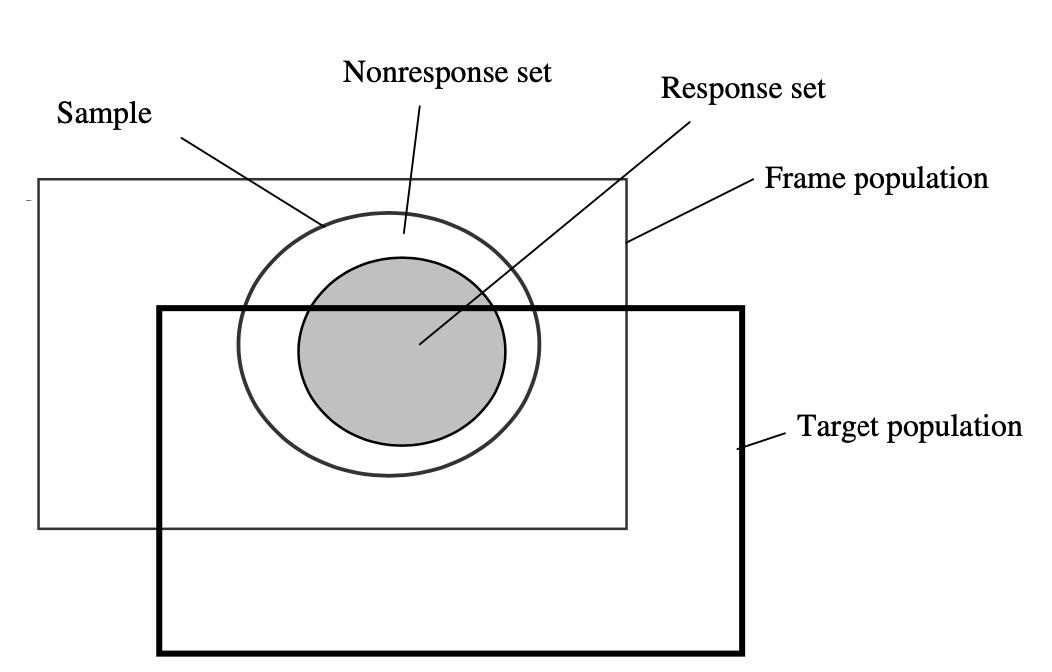
\includegraphics[width=0.8\textwidth]{fig-2-definicje/coverage.png}
% %         \caption{Błąd pokrycia i braki odpowiedzi. Źródło: Särndal, C. E., \& Lundström, S. (2005). Estimation in surveys with nonresponse. John Wiley \& Sons.}
% %     \end{figure}
% % \end{frame}

% % \begin{frame}{Główna idea -- źródła błędów w badaniach}
% %         \begin{figure}
% %         \centering
% %         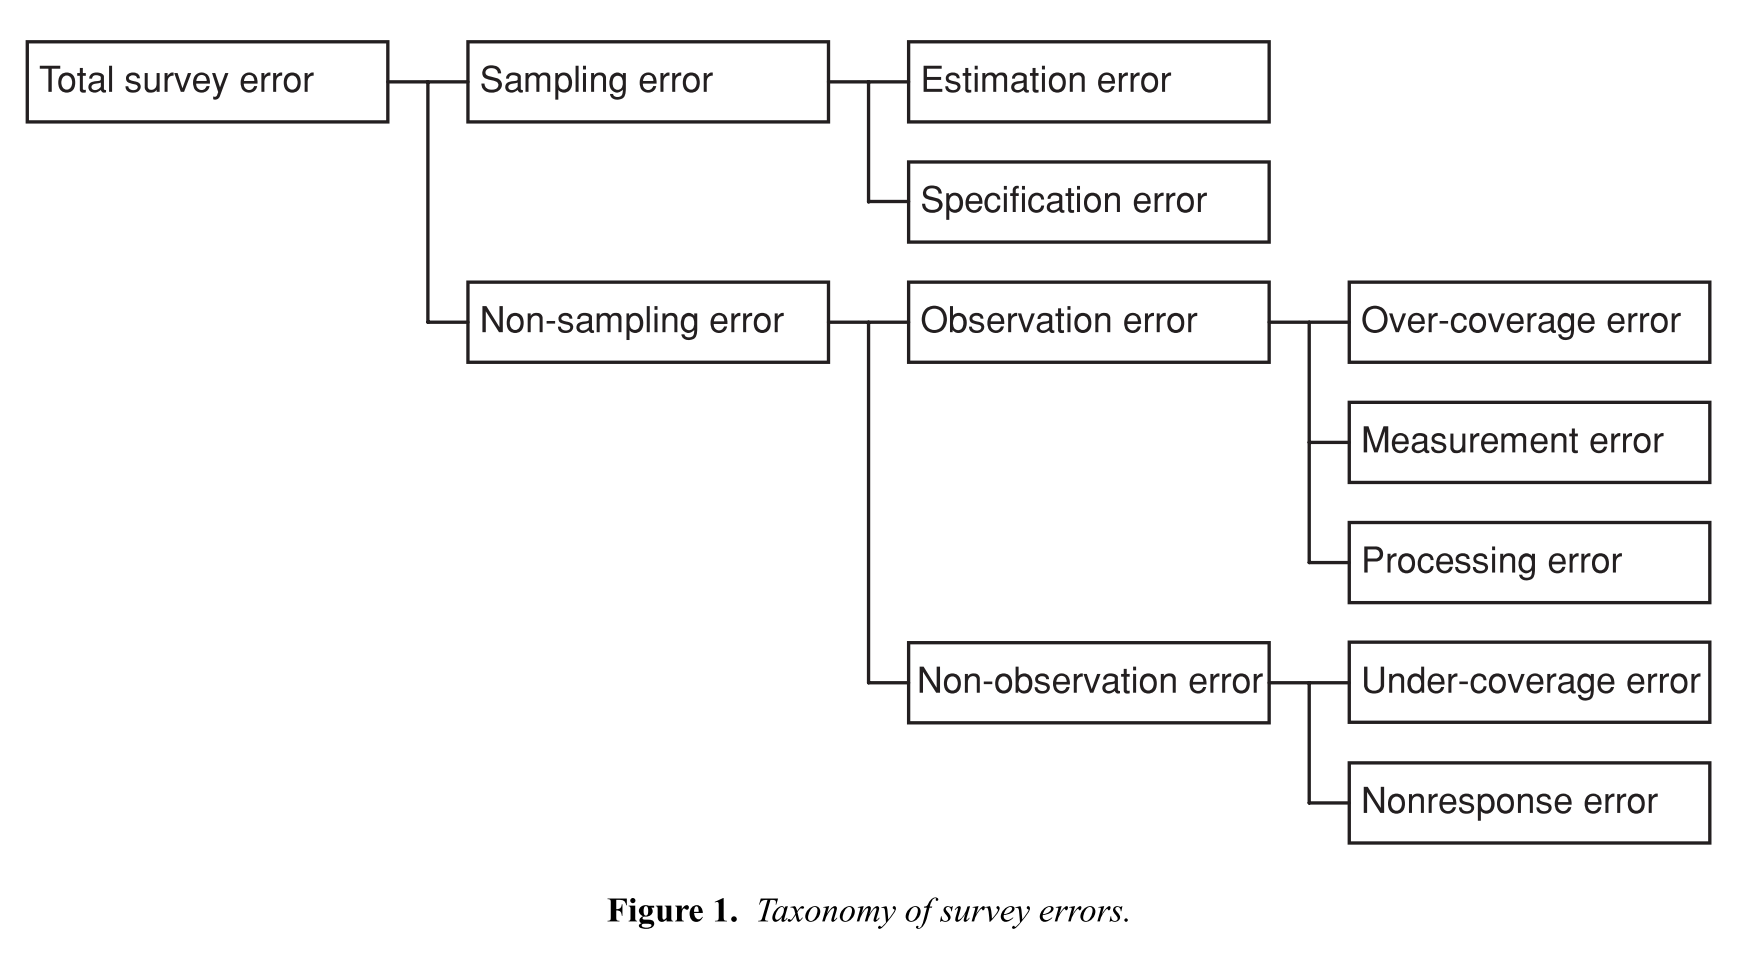
\includegraphics[width=0.9\textwidth]{fig-2-definicje/betlehem-errors.png}
% %         \caption{Taksonomia błędów w badaniach. Źródło: Bethlehem, J. (2010). Selection Bias in Web Surveys. International Statistical Review, 78(2), 161–188}
% %     \end{figure}
% % \end{frame}


% % \begin{frame}{Główna idea -- w praktyce trochę trudniejsze}
% %     \begin{figure}
% %         \centering
% %         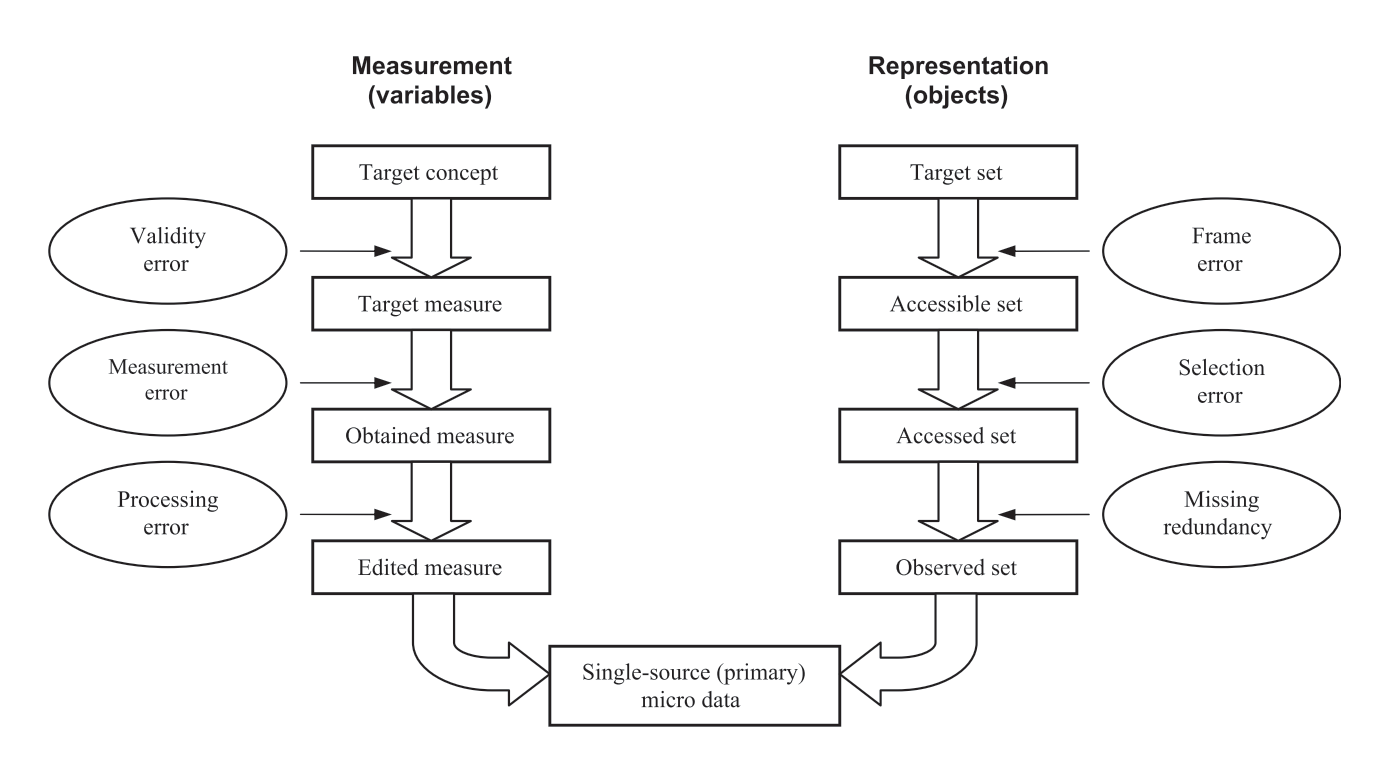
\includegraphics[width=0.9\textwidth]{fig-2-definicje/zhang1.png}
% %         \caption{Dwu fazowy cykl życia zintegrowanych mikrodanych statystycznych: Faza 1. Źródło: Zhang, L. (2012). Topics of statistical theory for register-based statistics and data integration. 66(1), 41–63.}
% %     \end{figure}
% % \end{frame}

% % \begin{frame}{Główna idea -- w praktyce trochę trudniejsze}
% %     \begin{figure}
% %         \centering
% %         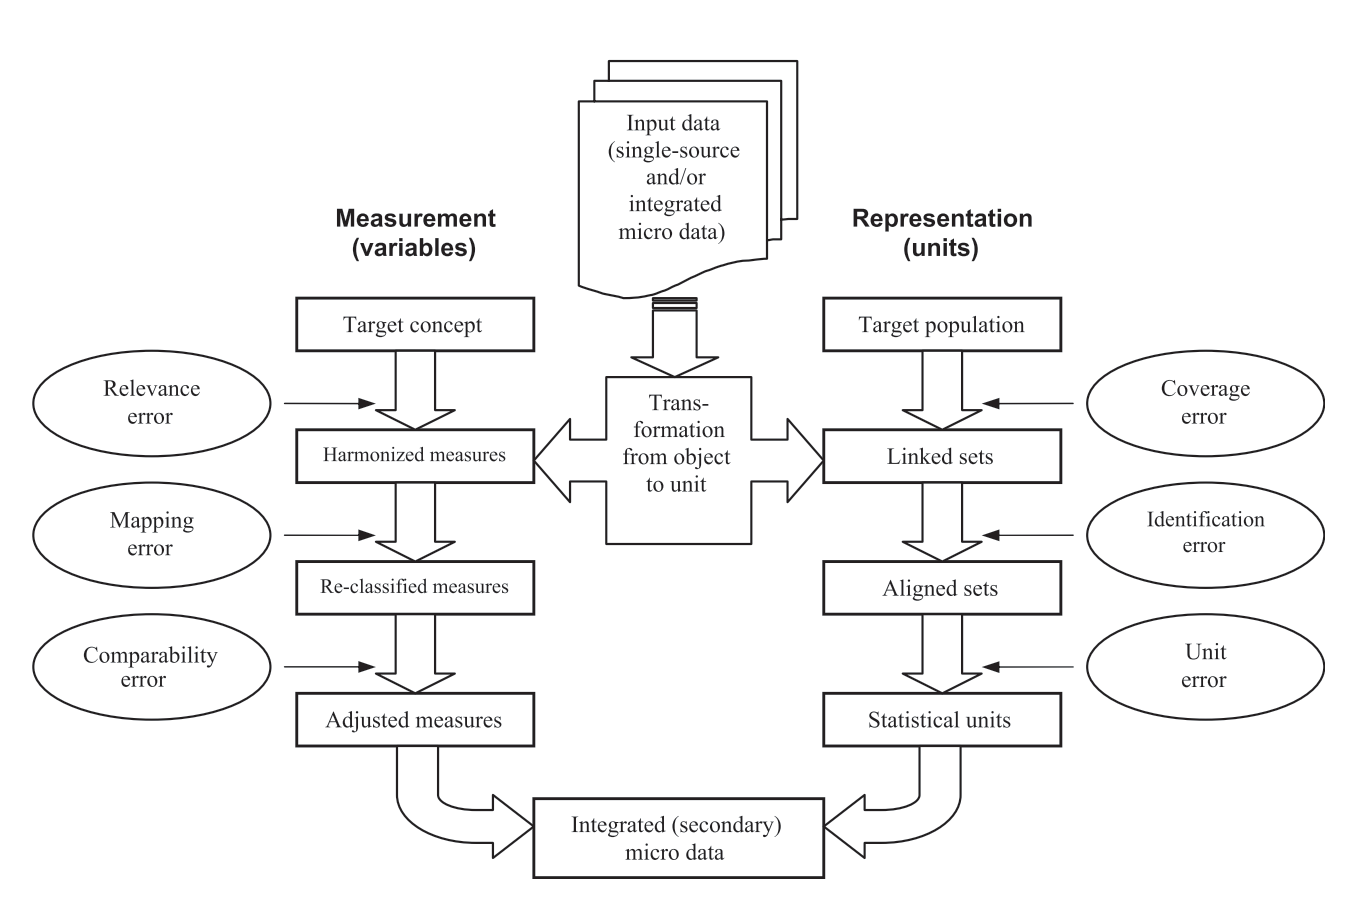
\includegraphics[width=0.9\textwidth]{fig-2-definicje/zhang2.png}
% %         \caption{Dwu fazowy cykl życia zintegrowanych mikrodanych statystycznych: Faza 2. Źródło: Zhang, L. (2012). Topics of statistical theory for register-based statistics and data integration. 66(1), 41–63.}
% %     \end{figure}
% % \end{frame}


% % \begin{frame}{Zadanie grupowe -- 15 minut}
% %  W kontekście źródeł nielosowych oraz powyższej klasyfikacji błędów proszę przedyskutować w grupach następujące sposoby badania:
 
% %  \begin{enumerate}
% %      \item \textbf{Grupa 1: badanie popyt na pracę (wolne miejsca pracy)} -- cel: oszacowanie ile firm oraz wolnych miejsc pracy jest w gospodarce.
% %      \item \textbf{Grupa 2: ceny najmu} -- cel: oszacowanie średniej ceny nieruchomości na wynajem,
% %      \item \textbf{Grupa 3: spędzanie wolnego czasu przez studentów} -- cel: oszacowanie struktury wolnego czasu czyli co robią studenci w wolnym czasie (np. \% na czytanie książek, \% na streaming itp),
% %      \item \textbf{Grupa 4: nastroje społeczeństwa} -- cel: określenia relacji między pozytywnymi, a negatywnymi nastrojami w społeczeństwie.
% %  \end{enumerate}
 
% % \end{frame}

% % \begin{frame}{Zadanie grupowe -- 15 minut}
% %  Dyskutując to zadania proszę wziąć pod uwagę:
% %  \begin{enumerate}
% %     \item jaką populację chcemy zbadać? co jest jednostką? co cechą?
% %      \item z jakich źródeł możemy (hipotetycznie) skorzystać? kto jest ich właścicielem?
% %      \item jakie jest pokrycie tych źródeł? czy obserwujemy tam tę samą populację, która nas interesuje?
% %      \item na jakie inne błędy nielosowe możemy się natknąć (np. błąd pomiaru, duplikaty)? 
% %      \item w jaki sposób moglibyśmy określić czy uzyskane szacunki są zbliżone do (nieznanych) wartości teoretycznych?
% %  \end{enumerate}
% %  Proszę przygotować krótką 1-2 slajdową prezentację.
% % \end{frame}


% % \subsubsection{Problematyka braków danych}

% % \begin{frame}{}
% %         \begin{center}
% %         \large
        
% %         A teraz szerzej, problematyka braków danych.
        
% %     \end{center}
% % \end{frame}

% % \begin{frame}{Big data, a problematyka braków danych}
% % \begin{itemize}
% %     \item Problem z big data możemy przedstawić w kontekście problemu braków danych.
% %     \item Powyższa sytuacja została przedstawiona na poniższym wykresie
% %     \begin{figure}
% %         \centering
% %         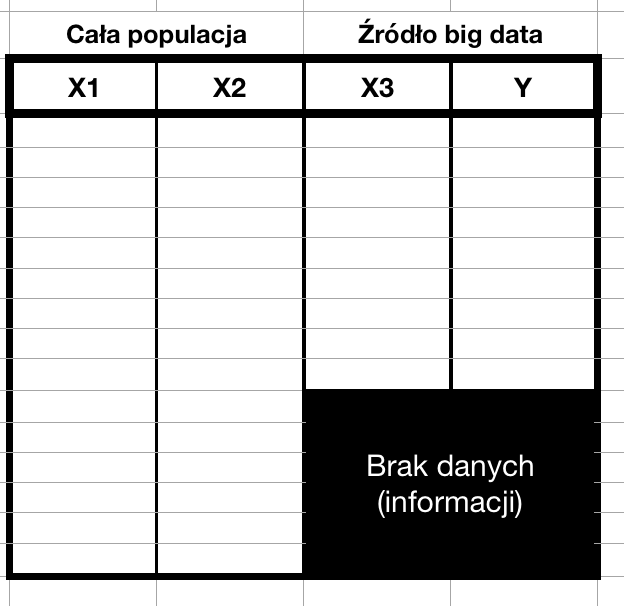
\includegraphics[width=0.4\textwidth]{figs/big-data-zrodlo.png}
% %     \end{figure}
% % gdzie $X1,X2$ są obserwowane dla całej populacji, a $X3$ i $Y$ są obserwowane wyłącznie w źródle big data. Na czarno zaznaczono część populacji, dla której nie mamy informacji.
% % \end{itemize}    
% % \end{frame}

% % \begin{frame}{Mechanizmy powstawania braków danych}
% % 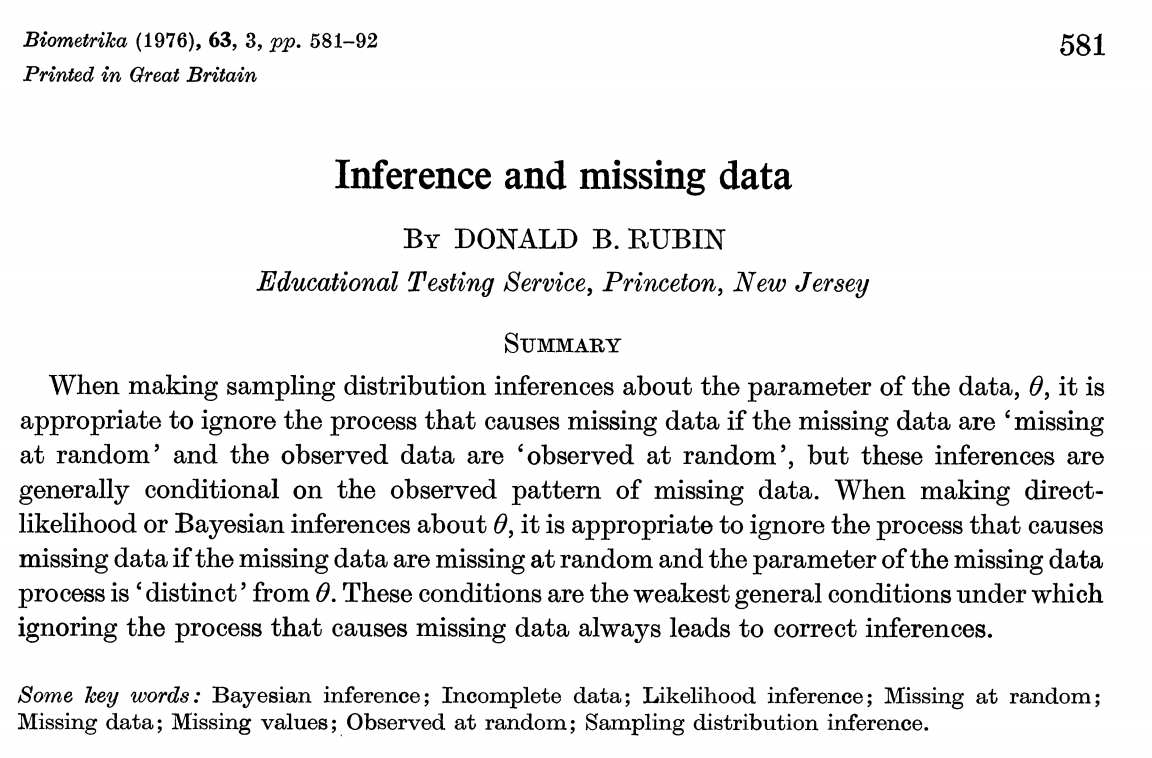
\includegraphics[width=\textwidth]{fig-2-definicje/rubin.png}
% % \end{frame}

% % \begin{frame}{Mechanizmy powstawania braków danych}
% % 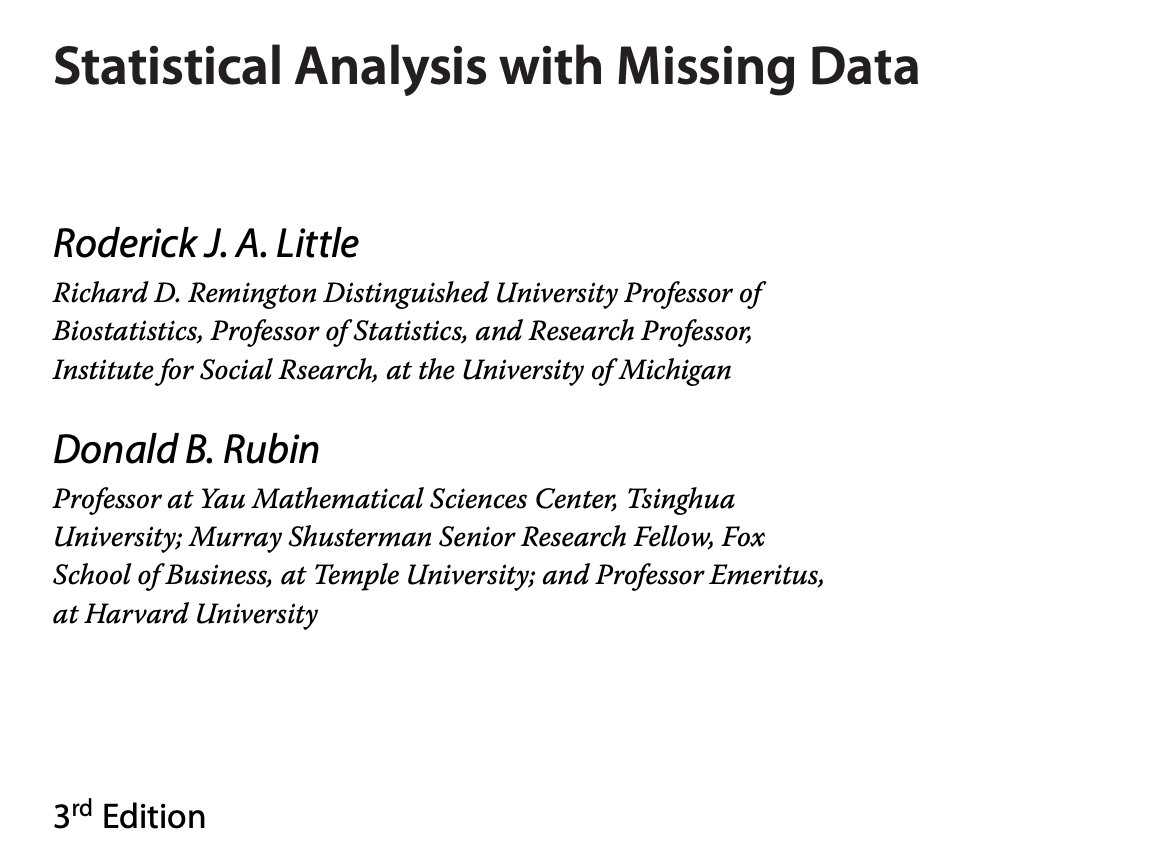
\includegraphics[width=\textwidth]{fig-2-definicje/rubin-little.png}
% % \end{frame}

% % \begin{frame}{Mechanizmy powstawania braków danych}
% % 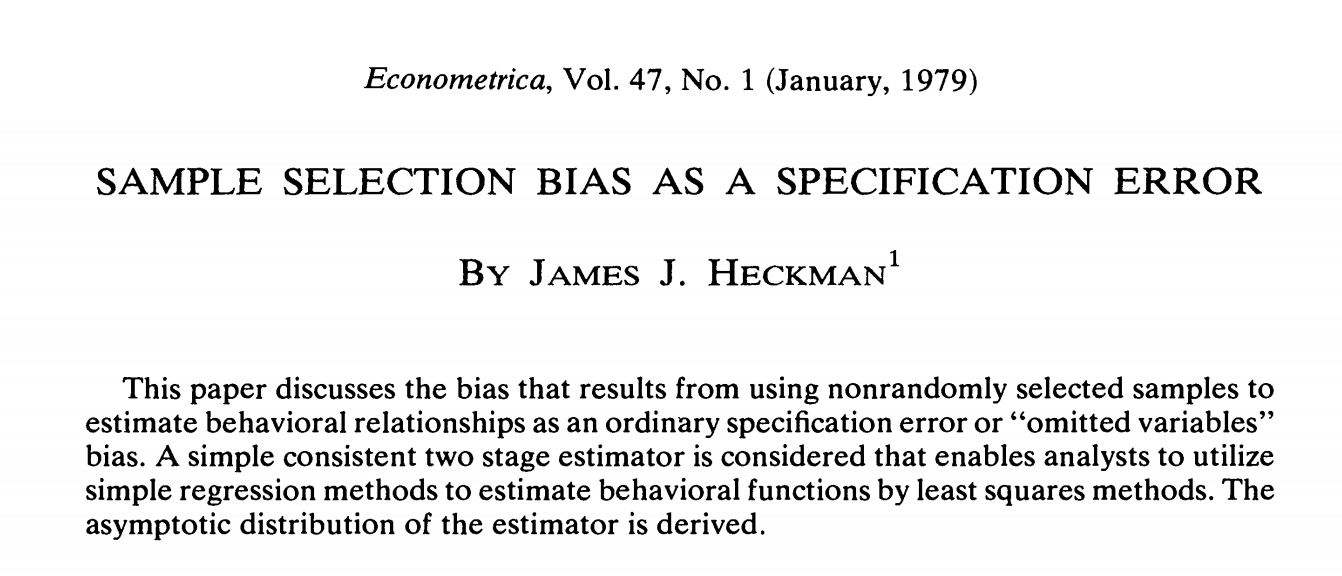
\includegraphics[width=\textwidth]{fig-2-definicje/heckman.png}
% % \end{frame}

% % \begin{frame}{Mechanizmy powstawania braków danych -- Rubin (1976)}
  
% %   Rubin (1976), Little i Rubin (2019) zdefiniował następujące mechanizmy braków danych:
% %   \begin{itemize}
% %       \item  Braki danych są całkowicie losowe (ang. \textit{Missing Completely at Random}, MCAR) -- \textbf{braki danych można pominąć}.
% %       \item Braki są losowe (ang. \textit{Missing at Random}, MAR)  -- \textbf{braków danych nie można pominąć, należy wykorzystać zmienne $X$ do korekcji ich wpływu} -- braki zależą od cech $X$,
% %       \item Braki danych nie są losowe (ang. \textit{Not Missing at Random}, NMAR) -- \textbf{braków danych nie można pominąć, należy zastosować bardzo zaawansowane metody} -- braki zależą od cech $X$ i $Y$.
% %   \end{itemize}  
% % \end{frame}

% % \begin{frame}{Mechanizmy powstawania braków danych}
% %  \begin{figure}
% %      \centering
% %      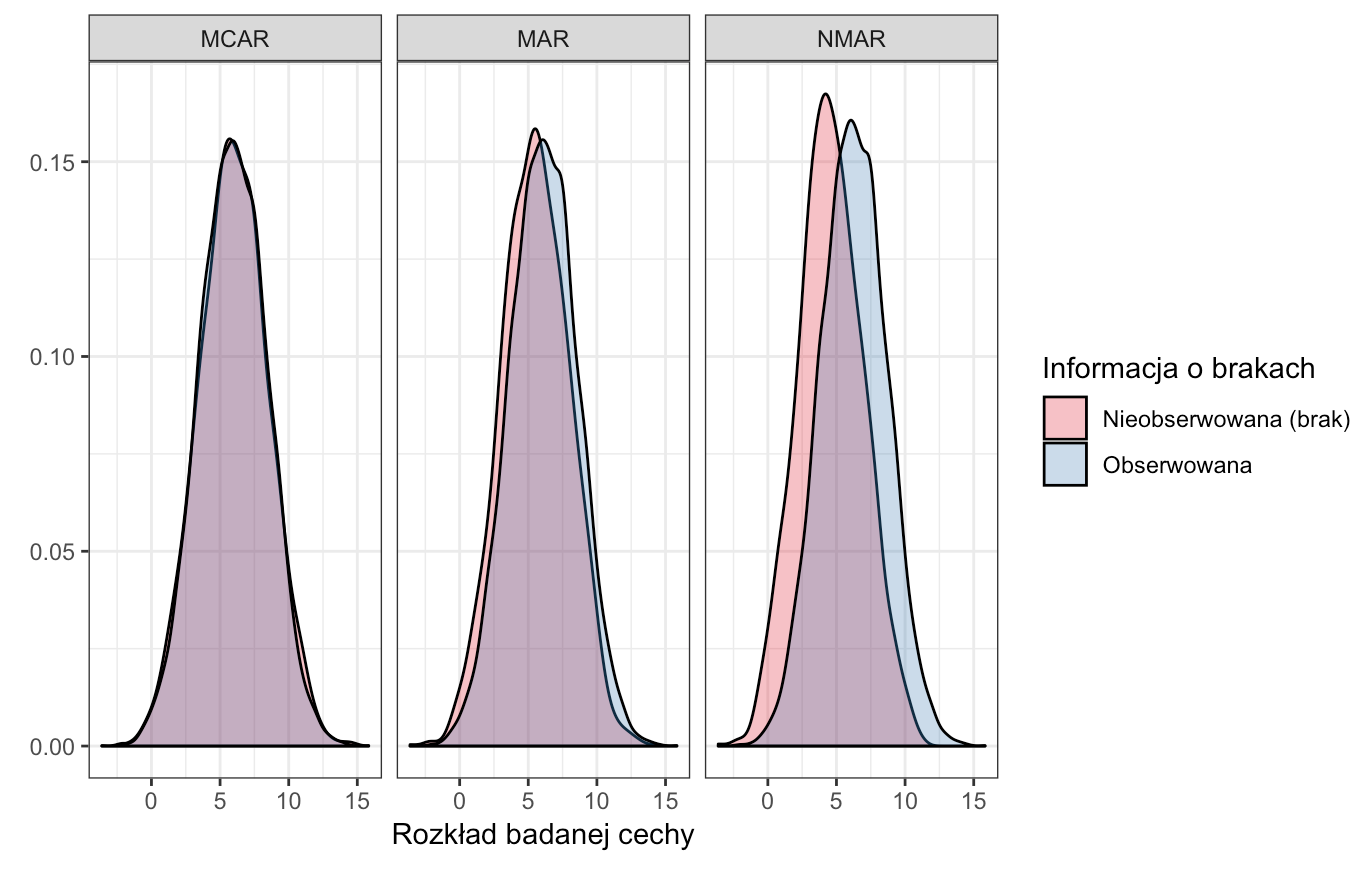
\includegraphics[width=\textwidth]{figs/nmar-r.png}
% %      \label{fig:my_label}
% %  \end{figure} 
% %  \end{frame}

% % \begin{frame}{Mechanizmy powstawania braków danych}
% % Dane były generowane zgodnie z następującym schematem

% % \begin{itemize}
% %     \item $X_1 \sim N(-2,1)$, $X_2 \sim N(4,1)$ -- niezależnie
% %     \item $Y \sim X_1 + X_2 + N(0,1)$
% % \end{itemize}
% % Następnie braki danych zostały wygenerowane zgodnie z następującymi schematami:
% % \begin{itemize}
% %     \item MCAR: $P(R=1) = \text{Bernoulli}(0.80)$
% %     \item MAR: $P(R=1) = \text{Bernoulli}( \exp(0.3*X_2)/(1 + \exp(0.3*X_2)))$ 
% %     \item MAR: $P(R=1) = \text{Bernoulli}( \exp(0.3*Y)/(1 + \exp(0.3*Y)))$ 
% % \end{itemize}
% %  \end{frame}


% % \begin{frame}{Mechanizmy powstawania braków danych -- rozkład ucięty}
% %  \begin{figure}
% %      \centering
% %      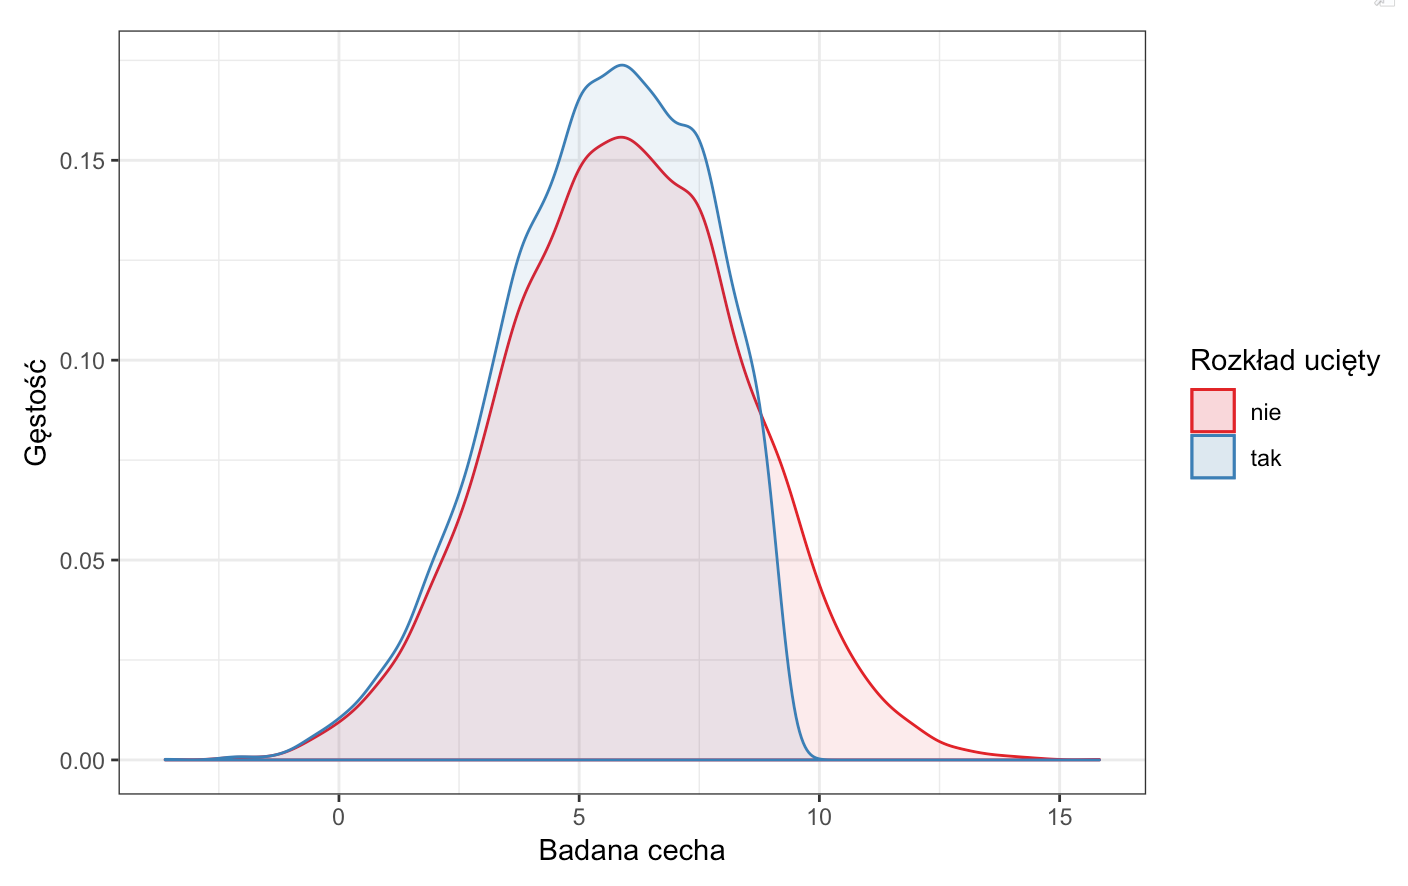
\includegraphics[width=\textwidth]{figs/rozklad-uciety.png}
% %      \label{fig:my_label}
% %  \end{figure} 
% %  \end{frame}


% % \begin{frame}{Mechanizmy powstawania braków danych}
% %  Inne przykłady za  Rubin (1976)
% %  \begin{figure}
% %      \centering
% %      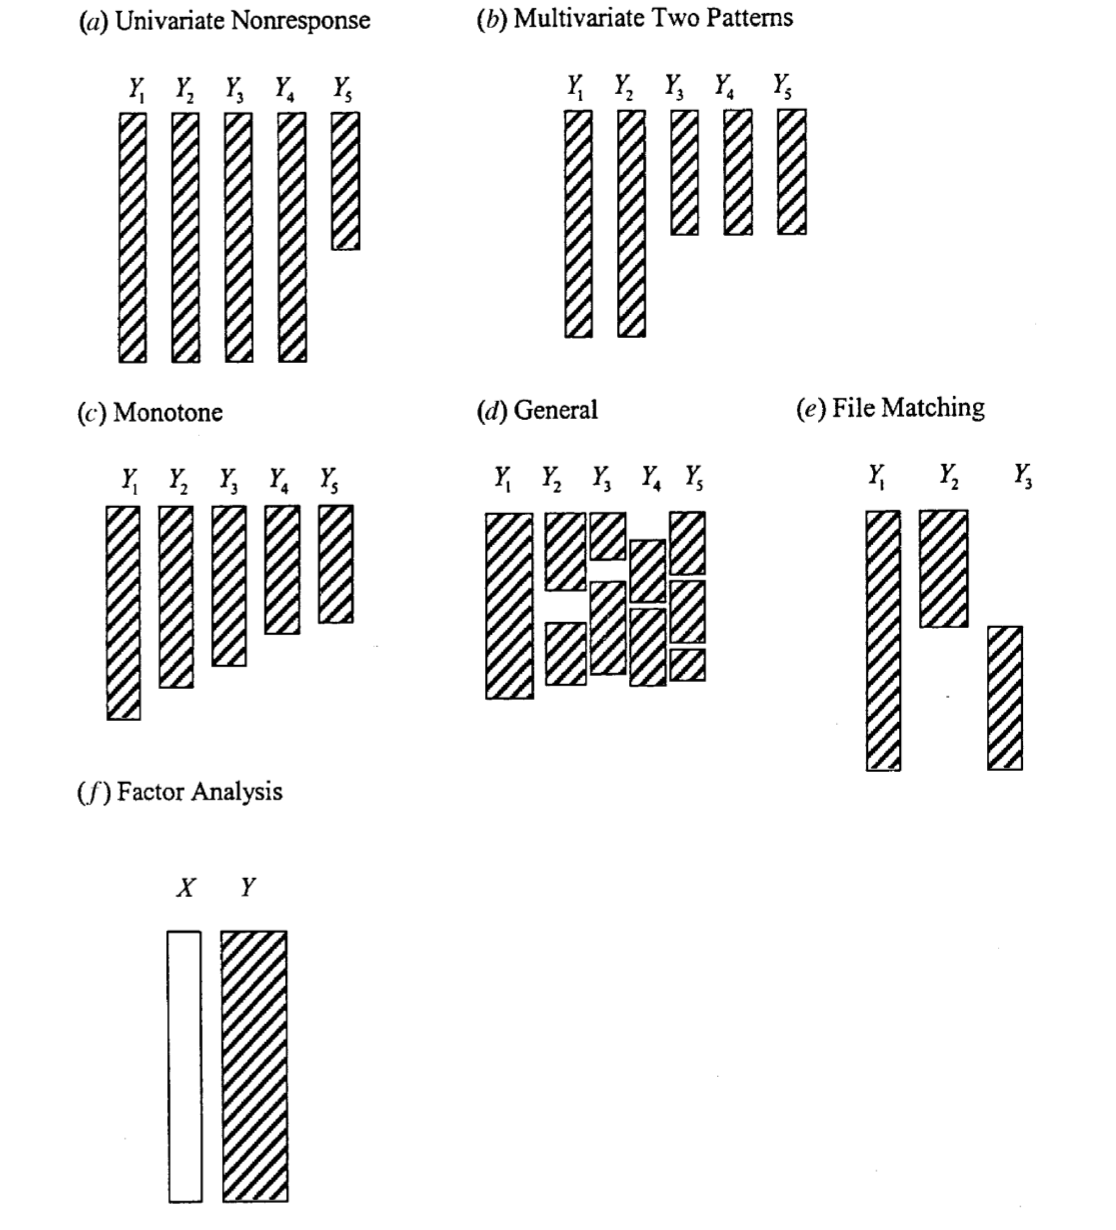
\includegraphics[width=0.6\textwidth]{figs/little-missing-data.png}
% %      \label{fig:my_label}
% %  \end{figure} 
% %  \end{frame}



% % % \begin{frame}{Przykład empiryczny -- wtórny rynek nieruchomości}
% % % \begin{itemize}
% % %     \item Badanie dotyczyło wtórnego rynku nieruchomości w Polsce w roku 2017.
% % %     \item Celem było określenie błędów pokrycia internetowych źródeł danych o wtórnym rynku nieruchomości (Gratka, OtoDom).
% % %     \item Porównania dokonano z danymi transakcyjnymi dla wszystkich powiatów w Polsce.
% % % \end{itemize}
% % % \end{frame}



% % % \begin{frame}{Przykład empiryczny -- wtórny rynek nieruchomości}
% % %  \begin{figure}
% % %      \centering
% % %      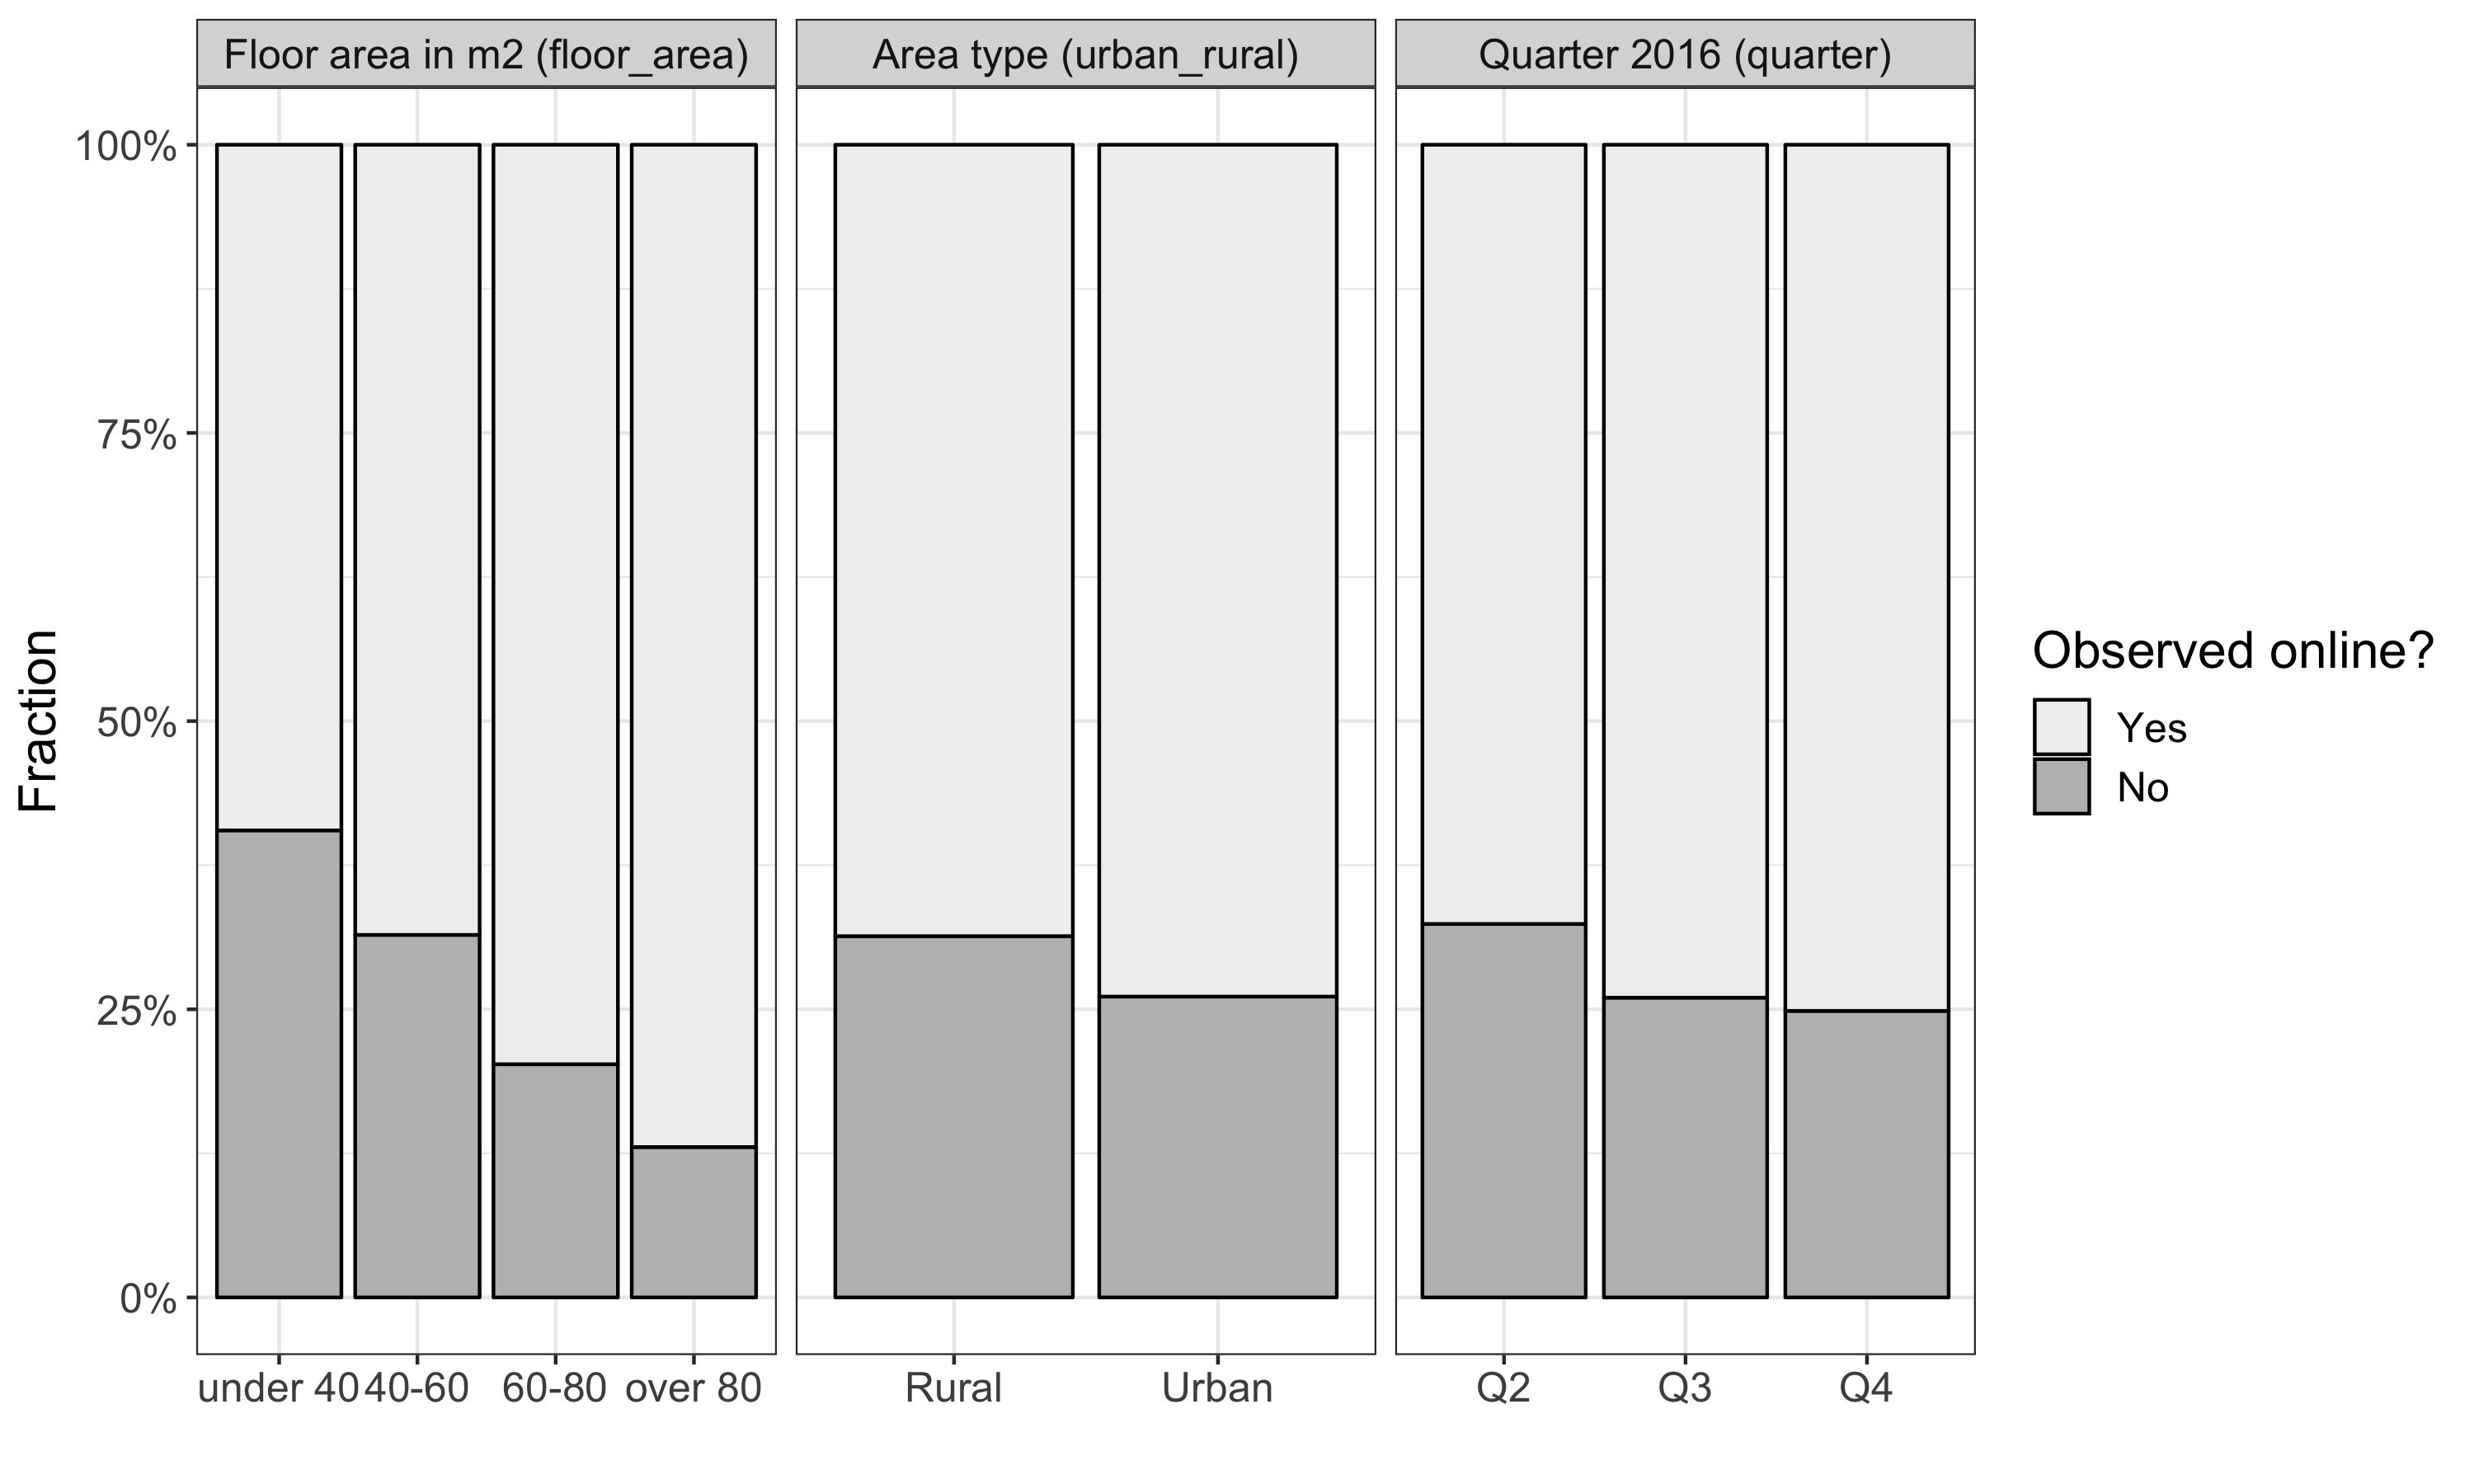
\includegraphics[width=\textwidth]{figs/cat-vars.jpg}
% % %      \label{fig:my_label}
% % %  \end{figure} 
% % % \end{frame}

% % % \begin{frame}{Przykład empiryczny -- wtórny rynek nieruchomości}
% % %  \begin{figure}
% % %      \centering
% % %      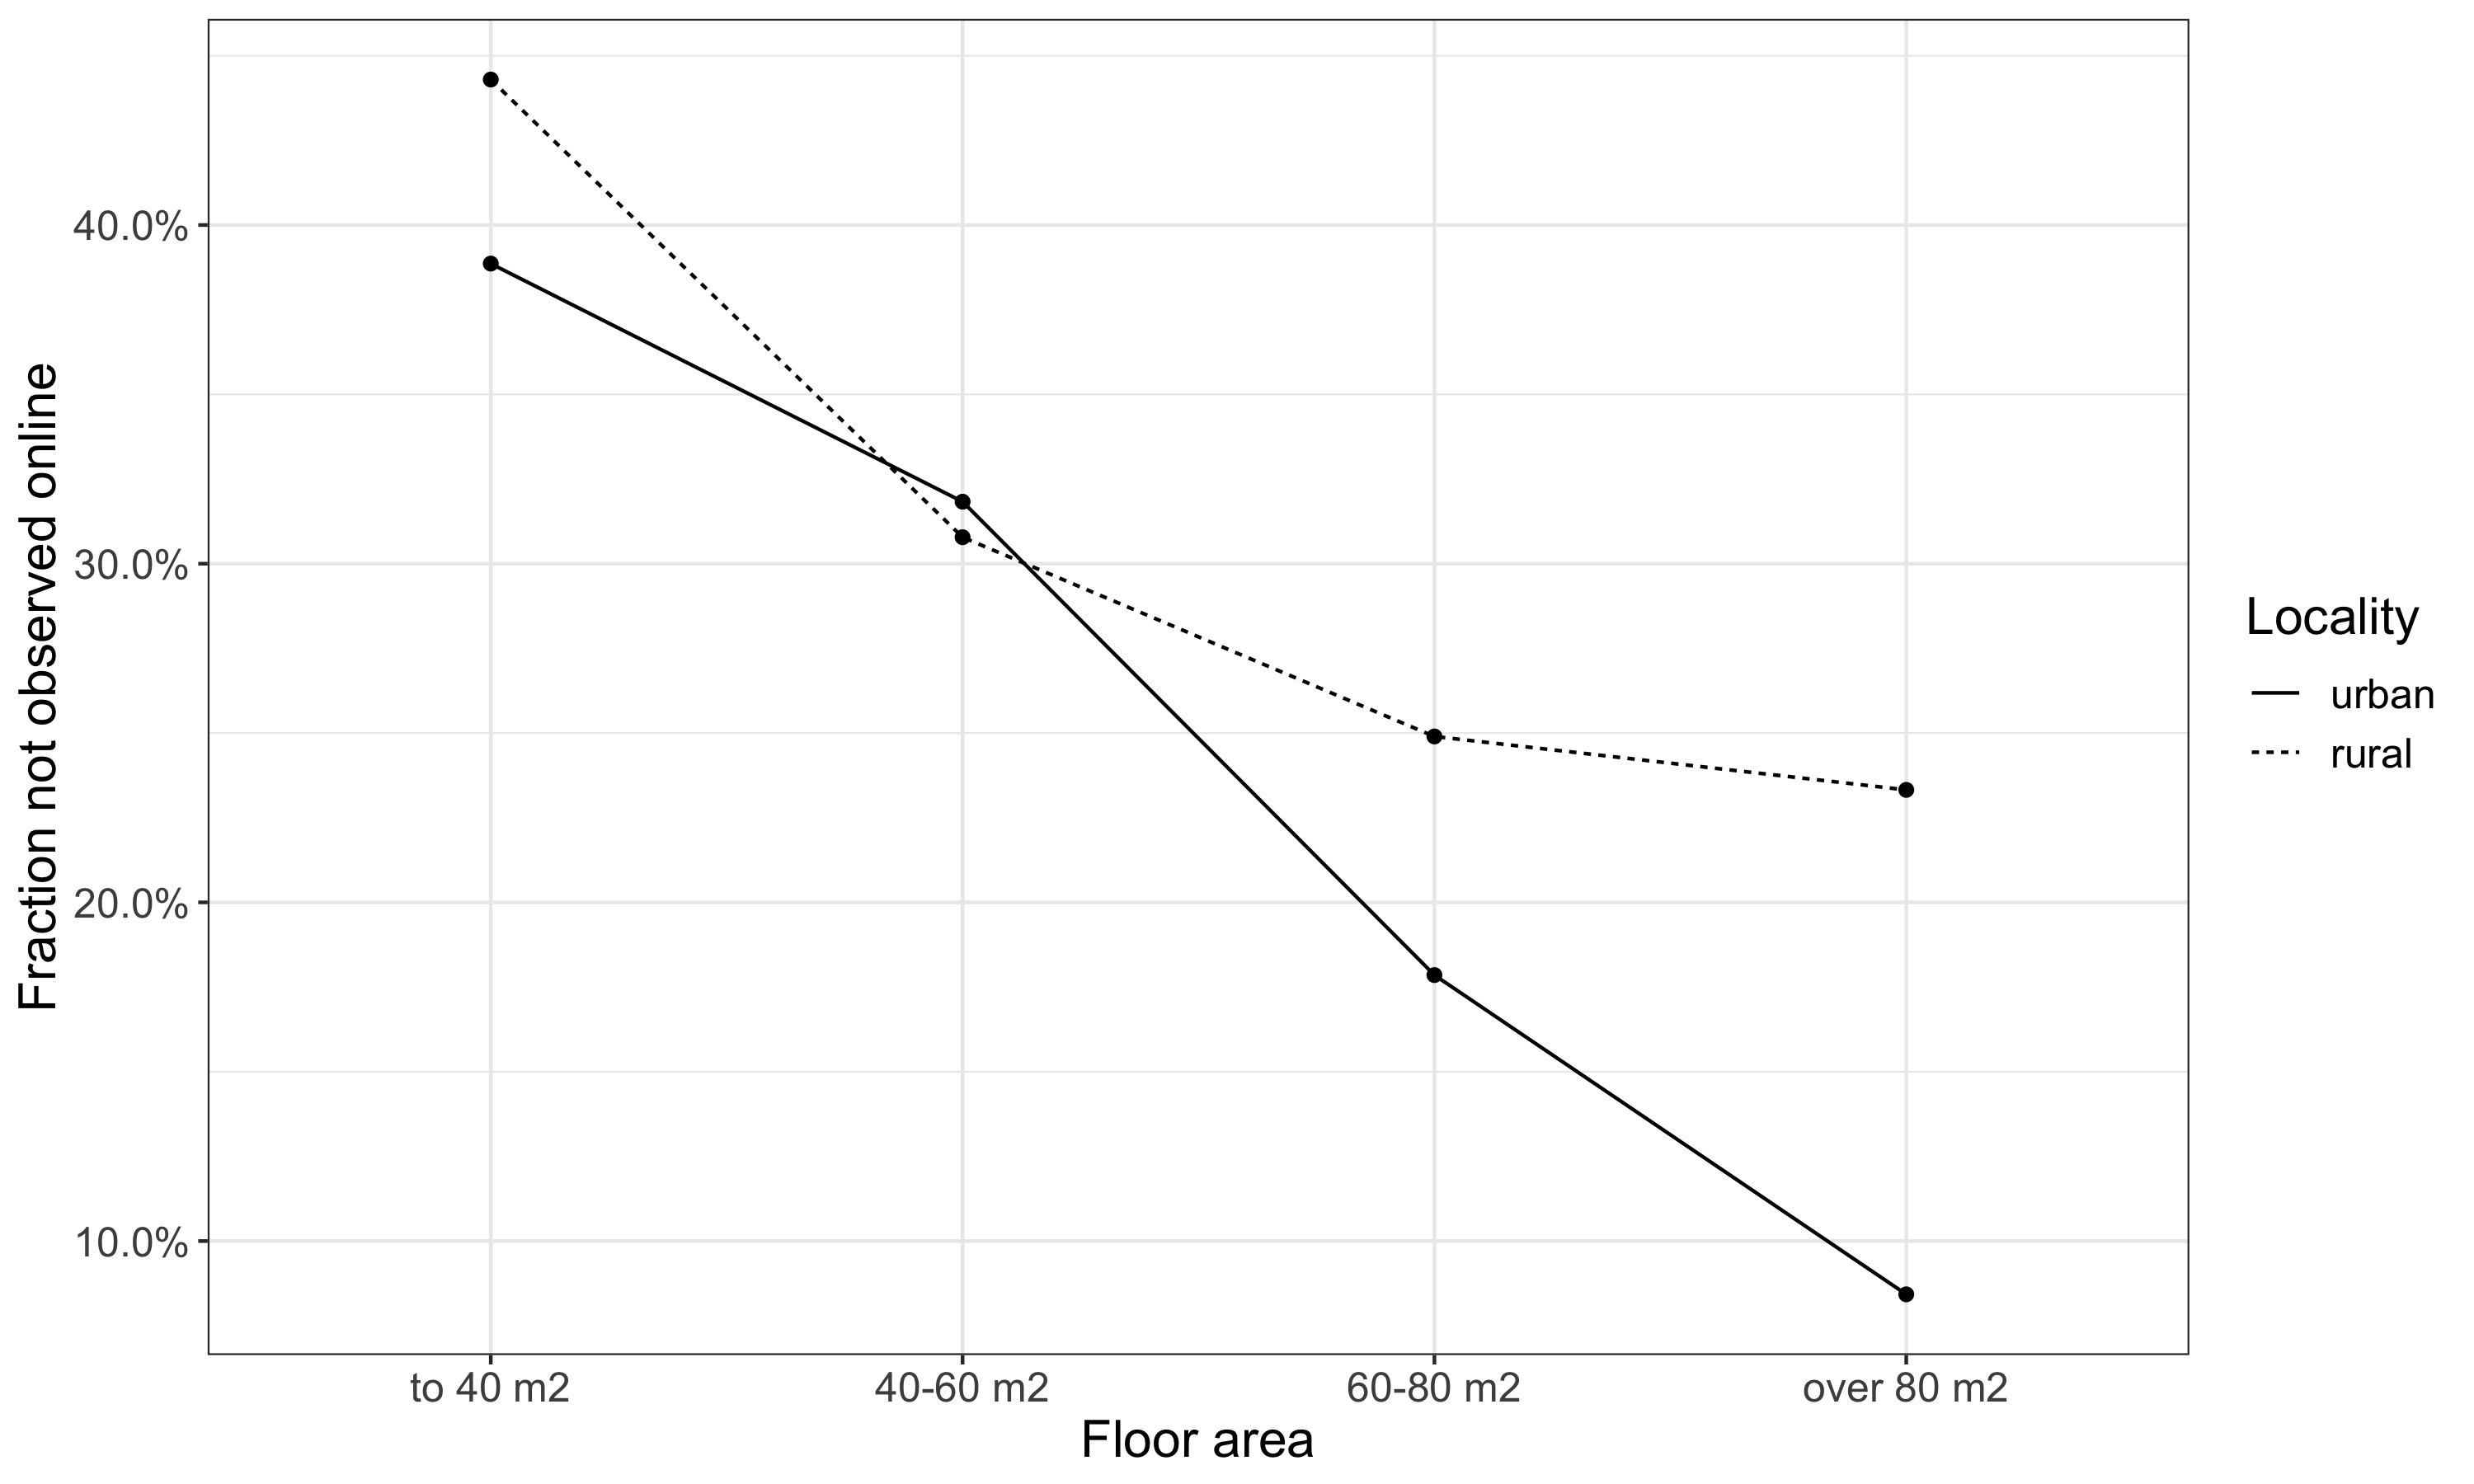
\includegraphics[width=0.8\textwidth]{figs/cat-locality.jpg}
% % %      \label{fig:my_label}
% % %  \end{figure} 
% % % \end{frame}

% % % \begin{frame}{Przykład empiryczny -- wtórny rynek nieruchomości}
% % %  \begin{figure}
% % %      \centering
% % %      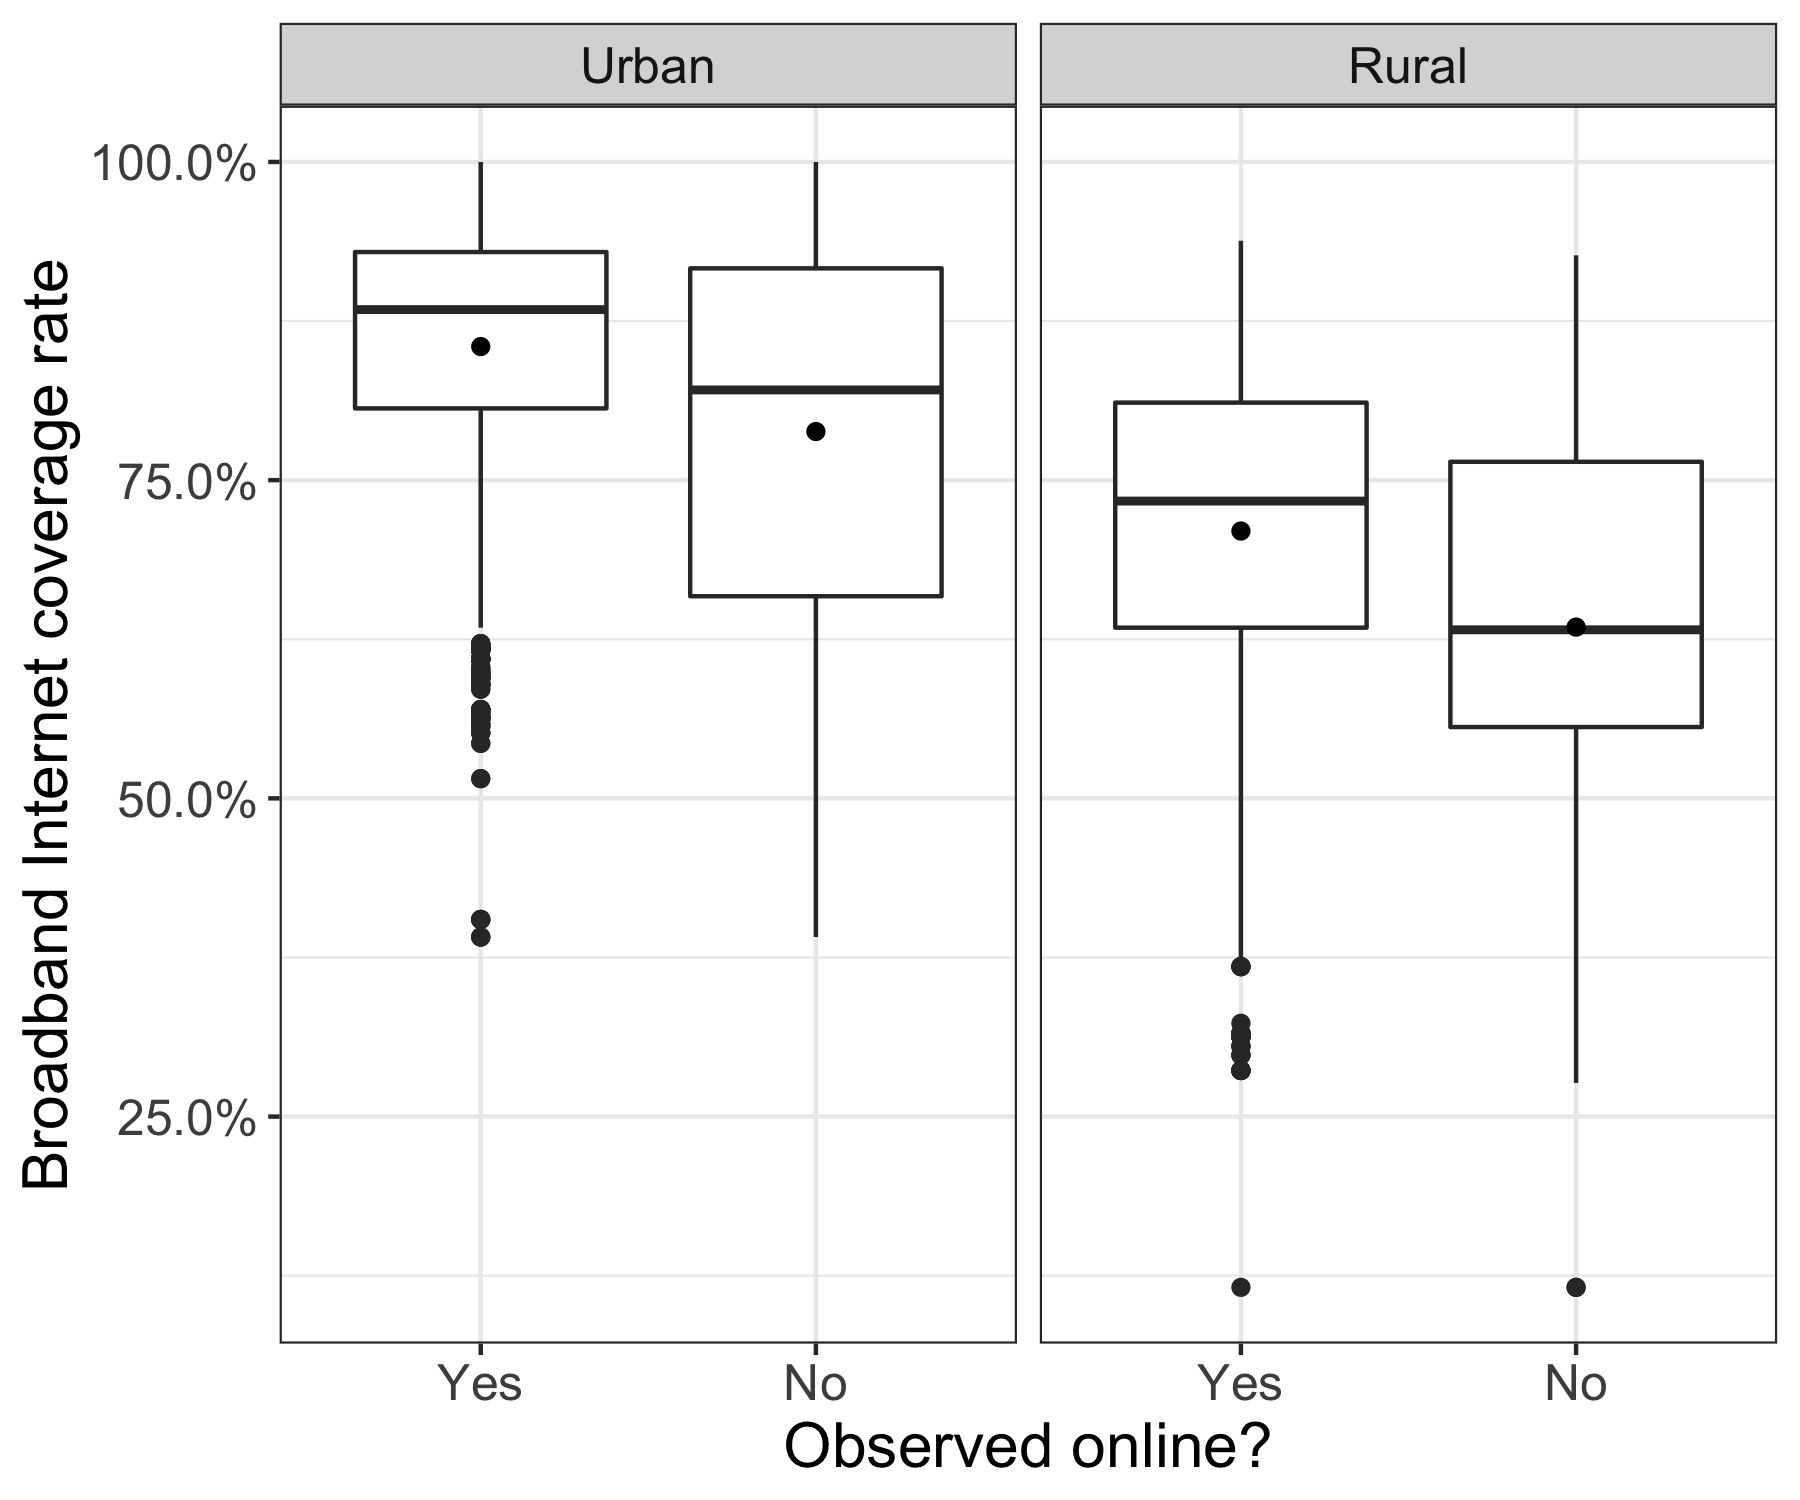
\includegraphics[width=0.8\textwidth]{figs/cont-internet-cov.jpg}
% % %      \label{fig:my_label}
% % %  \end{figure} 
% % % \end{frame}

% % % \begin{frame}{Przykład empiryczny -- wtórny rynek nieruchomości}
% % %  \begin{figure}
% % %      \centering
% % %      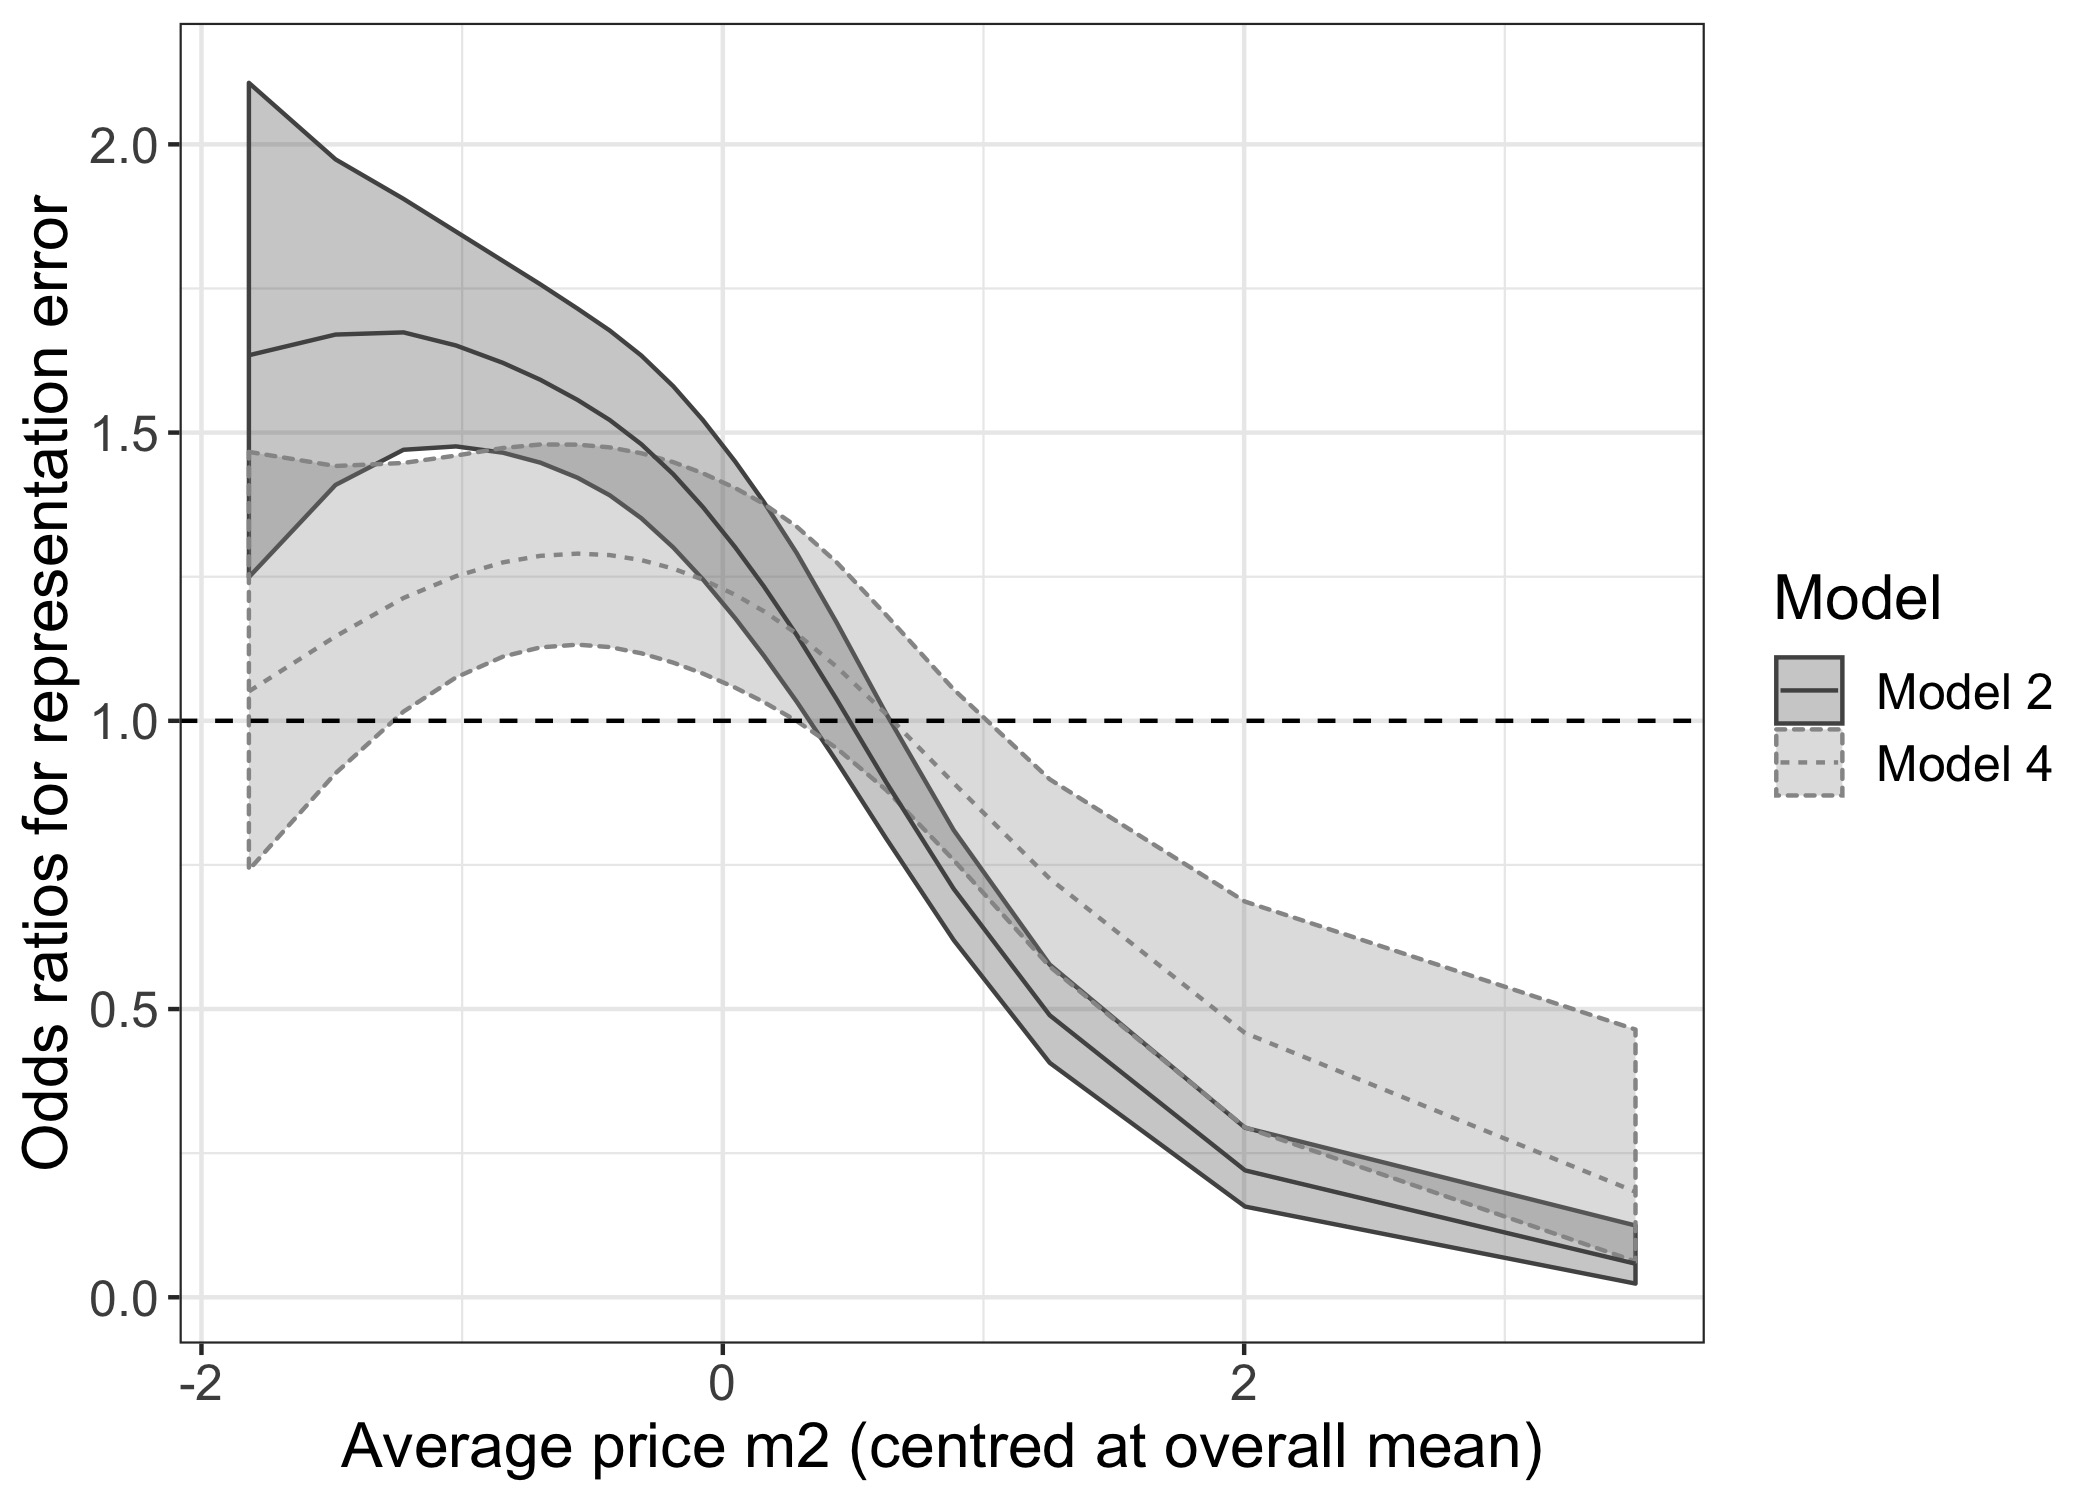
\includegraphics[width=0.8\textwidth]{figs/model-average.jpg}
% % %      \label{fig:my_label}
% % %  \end{figure} 
% % % \end{frame}


% % \begin{frame}{Ogólny wniosek}

% % \begin{center}
% %     \Large Nie skorygujemy błędów pokrycia czy autoselekcji bez dostępu do co najmniej jednego, niezależnego źródła danych (najlepiej próby losowej lub danych o populacji).
% % \end{center}
% % \end{frame}


% % % \begin{frame}{Przykład empiryczny}

% % % \begin{center}
% % % Przejdźmy do przykładu    
% % % \end{center}

% % % \end{frame}


\section{Metody estymacji dla prób nielosowych}

\begin{frame}{Metody estymacji -- rozważmy następujące przypadki}
    \begin{figure}
        \centering
        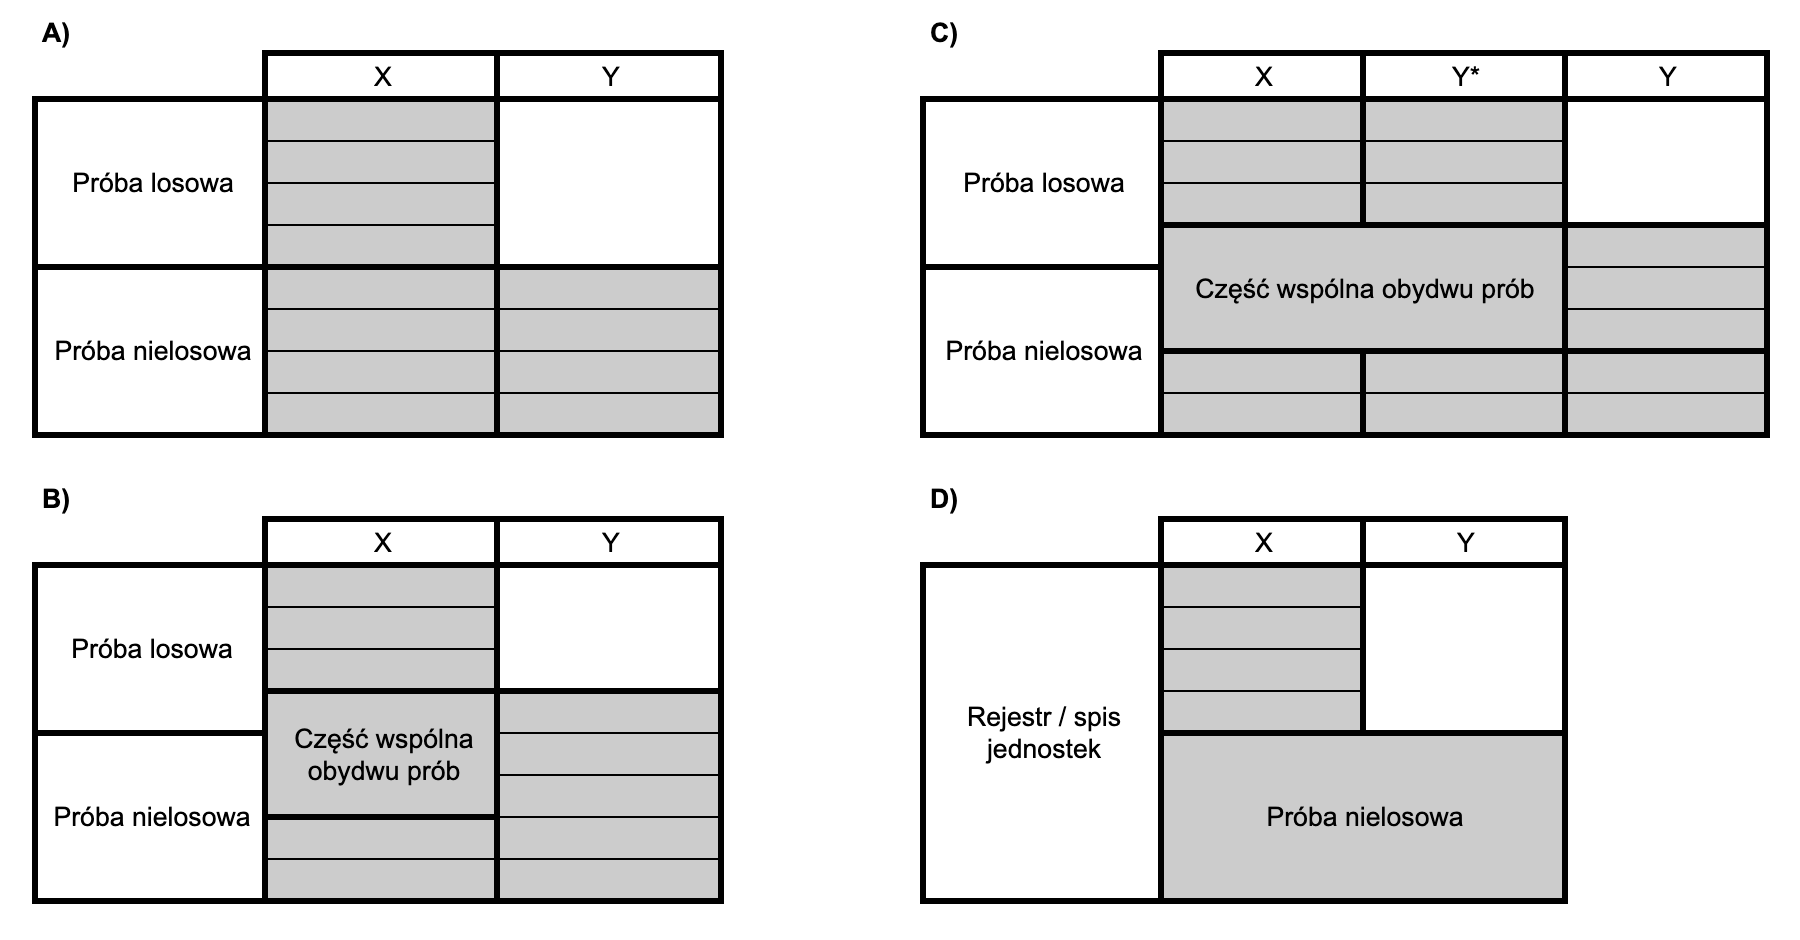
\includegraphics[width=\textwidth]{fig-4-meth/kombinacje-zrodel.png}
        \caption{Cztery przykładowe przypadki źródeł danych, gdzie celem jest oszacowanie wybranej charakterystyki cechy $Y$. Cechy $\bX$ są wspólne, cecha $Y^*$ to tzw. zmienna proxy.}
    \end{figure}
\end{frame}


\begin{frame}{Metody estymacji w przypadku prób nielosowych}
    \begin{center}
          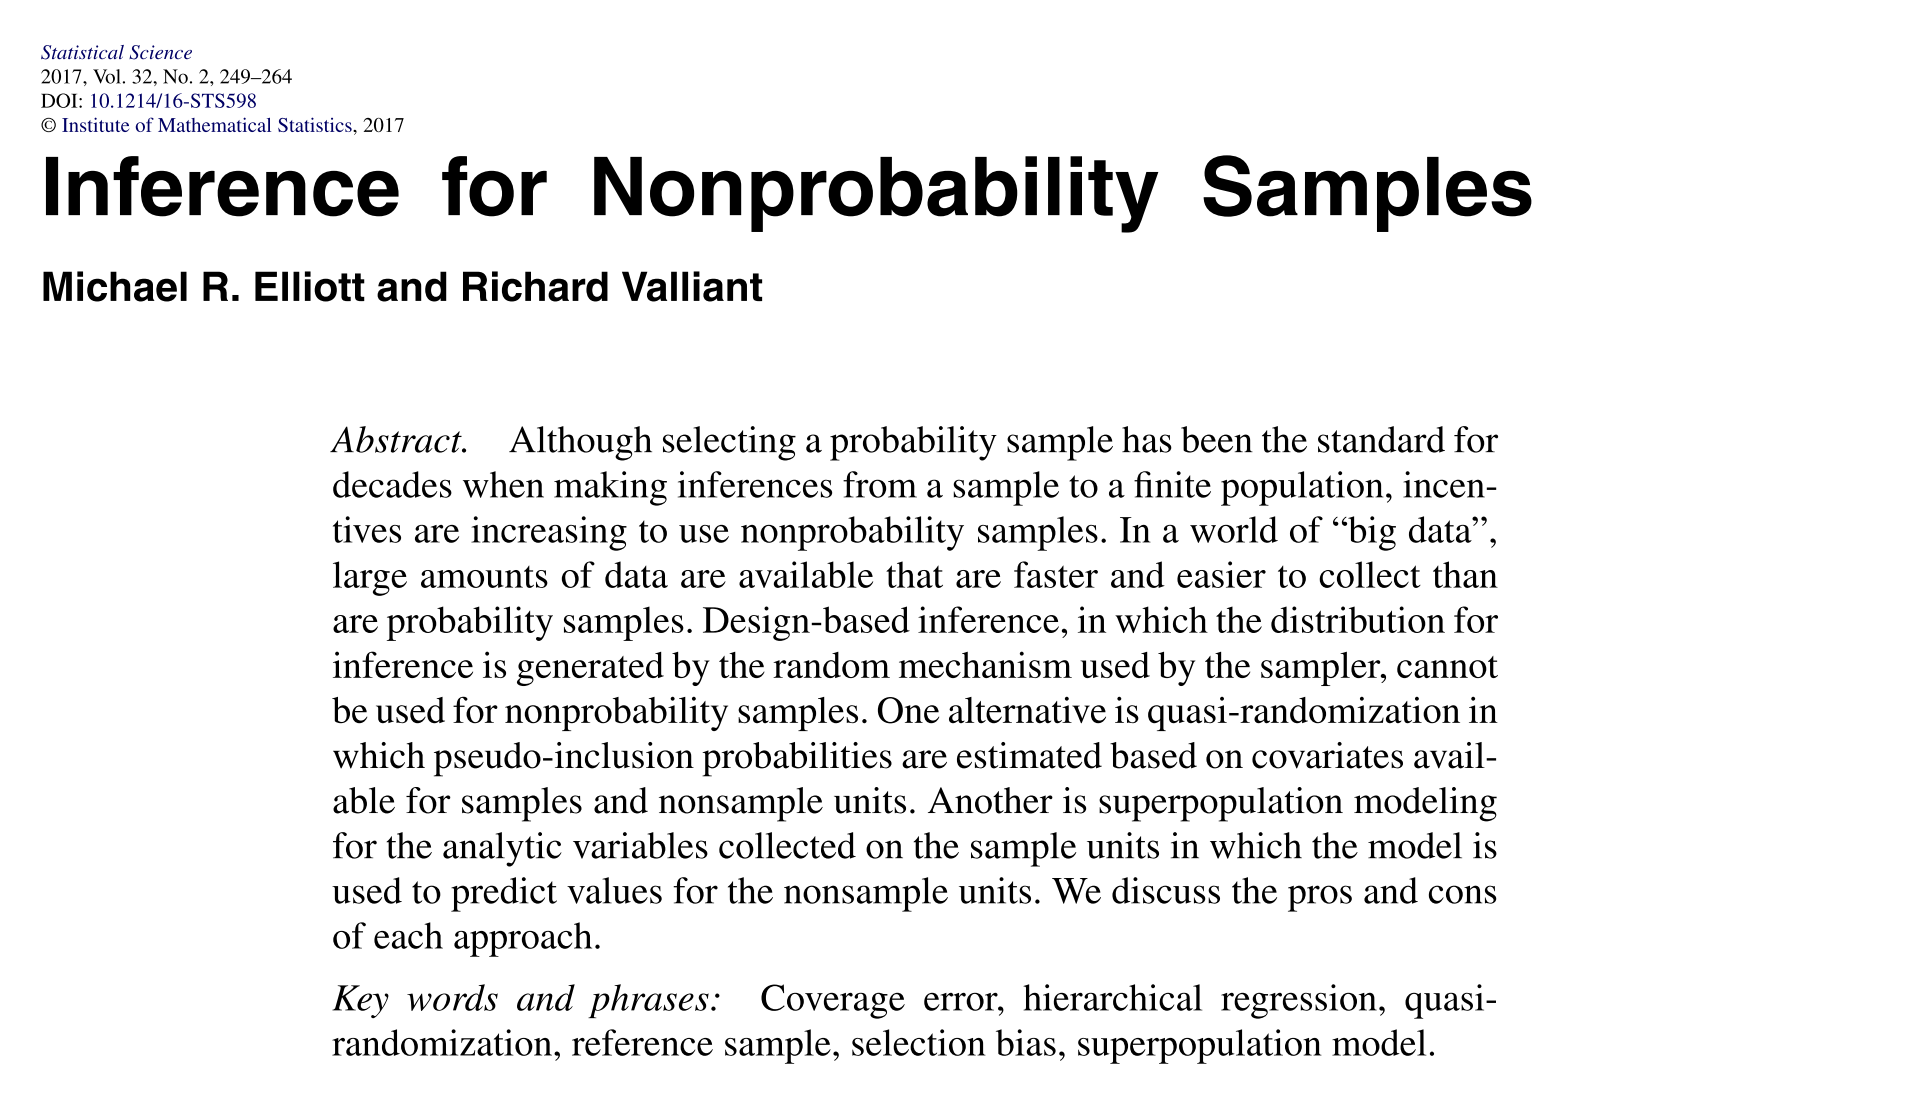
\includegraphics[width=\textwidth]{fig-4-meth/elliot-statsci.png}
    \end{center}
\end{frame}

\begin{frame}{Elliott i Valliant (2017) wyróżniają dwa podejścia:}
 \begin{itemize}
        \item \textbf{quasi-randomizacyjne} -- w której konstruujemy \textit{pseudo-wagi} z wykorzystaniem próby losowej lub znanych (albo estymowanych) wartości globalnych.
        \begin{center}
            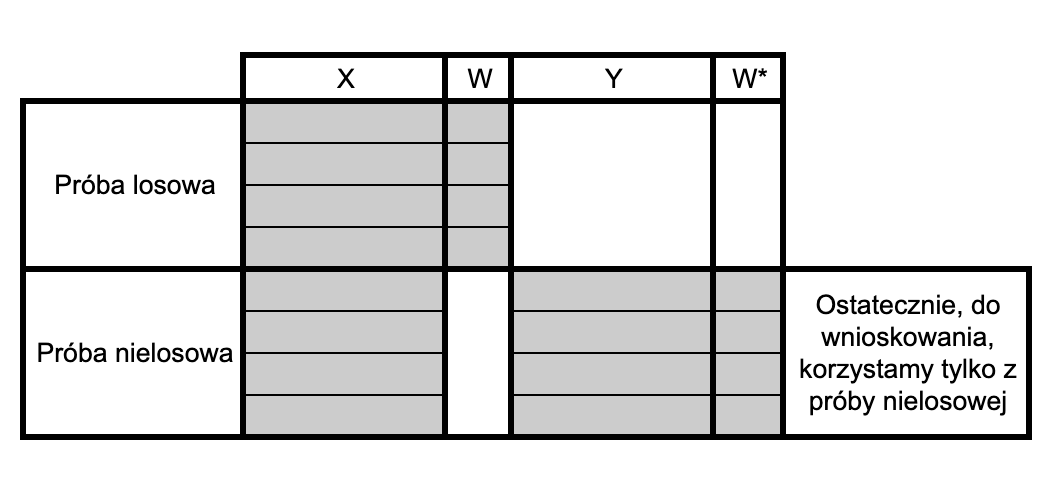
\includegraphics[width=0.55\textwidth]{fig-4-meth/pseudo-based.png}
        \end{center}
        \item \textbf{oparte na modelu} -- w którym zakładamy pewien model.
        \begin{center}
            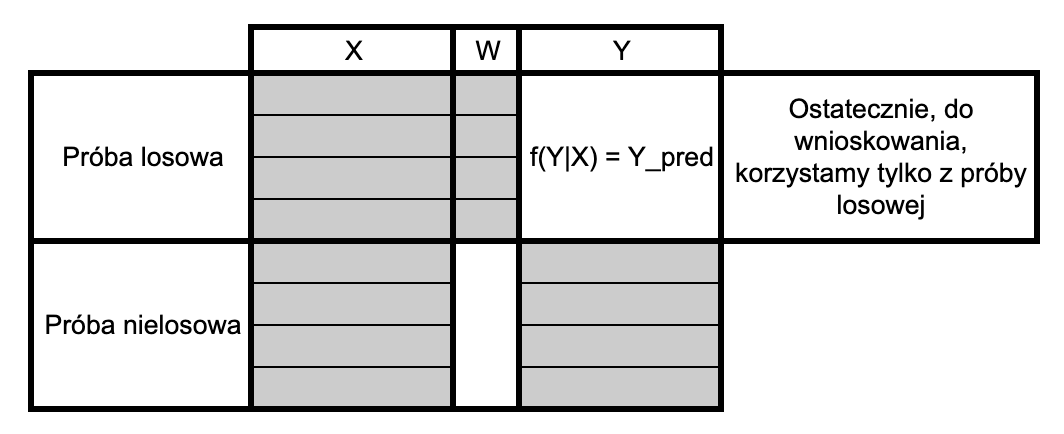
\includegraphics[width=0.55\textwidth]{fig-4-meth/model-based.png}
        \end{center}
    \end{itemize}
\end{frame}


\subsection{Podstawowe założenia na potrzeby zajęć} 


\begin{frame}{Podstawowe założenia}

\begin{itemize}
\justifying
    \item Niech $U=\{1,..., N\}$ oznacza populację docelową składającą się z $N$ oznaczonych jednostek. Każda jednostka $i$ ma powiązany wektor zmiennych pomocniczych $\bx_{i}$ oraz zmienną badaną $y_{i}$. 
     \begin{itemize}
        \item $\{ (y_i, \bx_i), i \in S_A\}$ - próba nielosowa $S_A$ o liczebności $n_A$
        \item $\left\{\left(\bx_i, \pi_{i}^B\right), i \in S_B\right\}$ - próba losowa $S_B$ o liczebności $n_B$
    \end{itemize}
    \item Dla próby losowej $S_B$ każda jednostka ma przypisaną wagę wynikającą z schematu losowania: $d_i^B = 1/\pi_i^B$, gdzie $\pi_i^B$ to prawdopodobieństwo włączenia.
    \item Naszym celem jest oszacowanie średniej w populacji $\mu_y=N^{-1}\sum_{i=1}^{N} y_{i}$ zmiennej $y$.
\end{itemize}

\end{frame}

% Slajd 2
\begin{frame}{Wskaźniki i prawdopodobieństwa włączenia}

\begin{itemize}
\justifying
    \item Wprowadźmy wskaźniki włączenia do prób, zdefiniowane dla wszystkich jednostek w populacji docelowej:
     \begin{itemize}
        \item $R_i^A=I(i \in S_A)$ - włączenie do próby nielosowej $S_A$
        \item $R_i^B=I(i \in S_B)$ - włączenie do próby losowej $S_B$
    \end{itemize}
    \item Niech $\pi_i^A=P(R_i^A=1 \mid \bx_i, y_i)=P(R_i^A=1 \mid \bx_i)$ będzie prawdopodobieństwem włączenia (propensity score), które charakteryzuje mechanizm doboru próby $S_A$.
    \item W przeciwieństwie do $\pi_i^B$, wartości $\pi_i^A$ i odpowiadające im wagi $d_i^A=1/\pi_i^A$ są nieznane.
\end{itemize}
    
\end{frame}

\begin{frame}{Struktura danych}
    \begin{table}[ht!]
        \centering
        \resizebox{\linewidth}{!}{
        \begin{tabular}{llcccc} 
        \hline
        Próba & ID & Włączenie ($R$) & Waga ($d$) & Zmienne pom. ($\bx$) & Zm. badana ($y$) \\
        \hline
        Nielosowa  & 1 & 1 & ? & $\checkmark$ & $\checkmark$ \\ 
        $S_A$ & $\vdots$ & $\vdots$ & $\vdots$ & $\vdots$ & $\vdots$ \\
        & $n_A$ & 1 & ? & $\checkmark$ & $\checkmark$ \\
        Losowa  & 1 & 0 & $\checkmark$ & $\checkmark$ & ? \\
        $S_B$ & $\vdots$ & $\vdots$ & $\vdots$ & $\vdots$ & $\vdots$ \\ 
        & $n_B$ & 0 & $\checkmark$ & $\checkmark$ & ? \\                                     
        \hline     
        \end{tabular}
        }
        \caption{Struktura danych w układzie dwóch prób}
    \end{table}
    
    Wartości zmiennej $y_i$ nie są obserwowane w próbie losowej, więc nie można ich bezpośrednio wykorzystać do oszacowania badanej wielkości. Zamiast tego, próbujemy łączyć próbę nielosową i losową.
\end{frame}

\begin{frame}{Główne założenia}
    Ze względu na brak uniwersalnie przyjętej metody łączenia prób, założenia różnią się znacznie. Jednak dla większości metod przyjmuje się następujące główne założenia:
    
    \begin{itemize}
    \justifying
        \item[A1] $R_i^A$ i zmienna badana $y_i$ są niezależne przy ustalonym zbiorze zmiennych pomocniczych $\bx_i$ (mechanizm MAR).
        \item[A2] Wszystkie jednostki w populacji docelowej mają niezerowe prawdopodobieństwo włączenia do próby nielosowej, tj. $\pi_i^A>0$, $i=1,2, \ldots, N$ (brak błędu pokrycia).
        \item[A3] Wskaźniki włączenia $R_1, R_2, \ldots, R_N$ są niezależne przy ustalonym zbiorze zmiennych pomocniczych $\left(\bx_1, \bx_2, \ldots, \bx_N\right)$ (brak grupowania).
    \end{itemize}
    
    Obecnie pomijamy nakładanie się prób $S_A$ i $S_B$ oraz zakładamy brak błędów pomiaru w $y_i$ i znajomość wartości $\bx_i$.
\end{frame}

\subsection{Metody quasi-randomizacyjne}

\begin{frame}{Propensity score -- Rosenbaum \& Rubin (1983)}
\begin{center}
    
\includegraphics[width=\textwidth]{fig-4-meth/rubin.png}
\end{center}
\end{frame}

\begin{frame}{Propensity score  -- Lee (2006)}
\begin{center}
    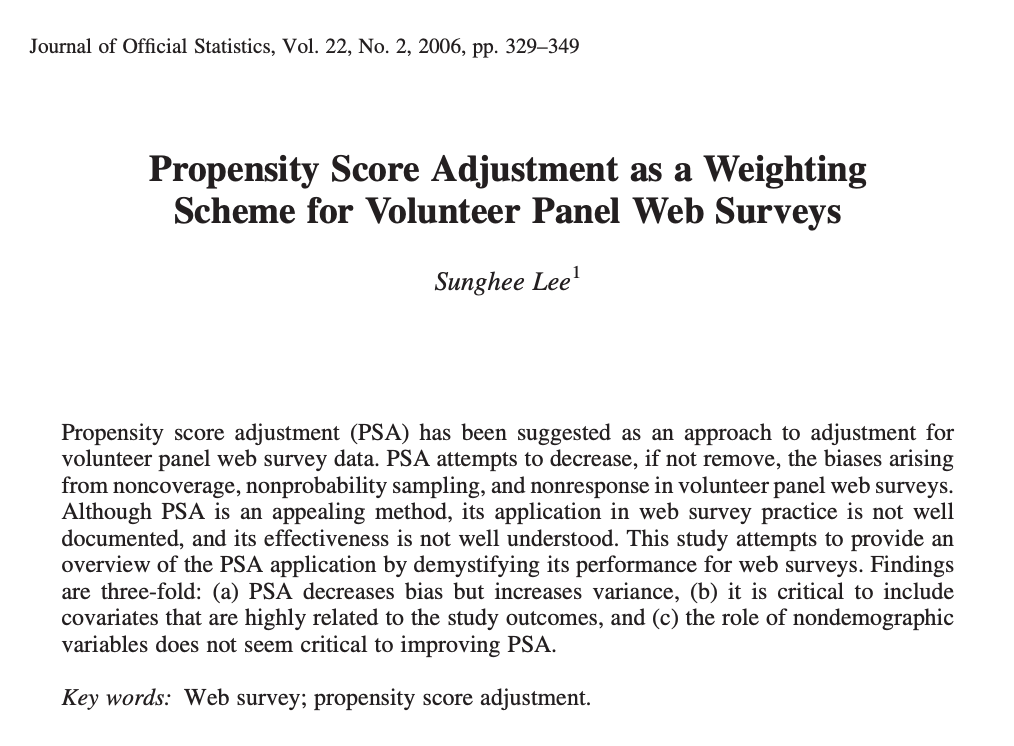
\includegraphics[width=\textwidth]{fig-4-meth/lee.png}
\end{center}
\end{frame}

\begin{frame}{Propensity score  -- Chen (2020)}
\begin{center}
    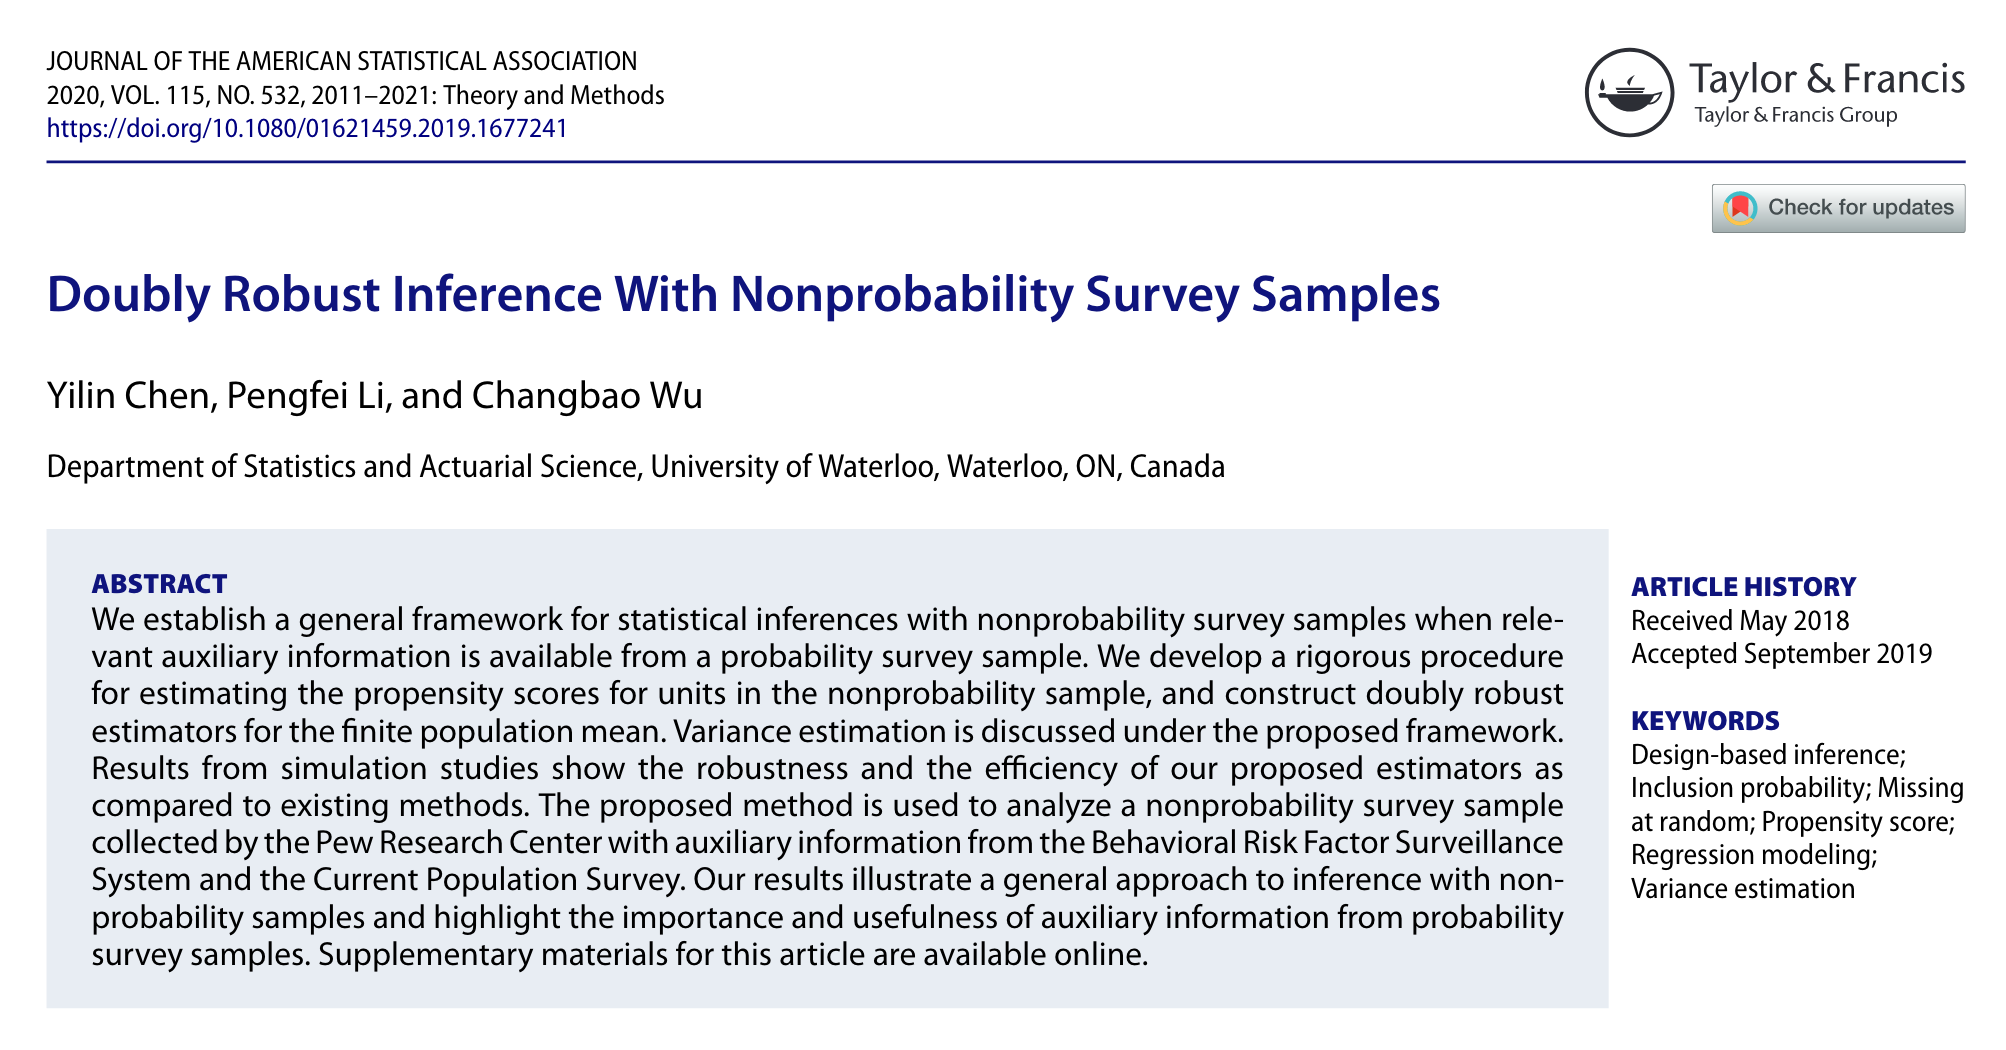
\includegraphics[width=\textwidth]{fig-4-meth/ps-dr.png}
\end{center}
\end{frame}

\begin{frame}{Propensity score  -- Wu (2022)}
\begin{center}
    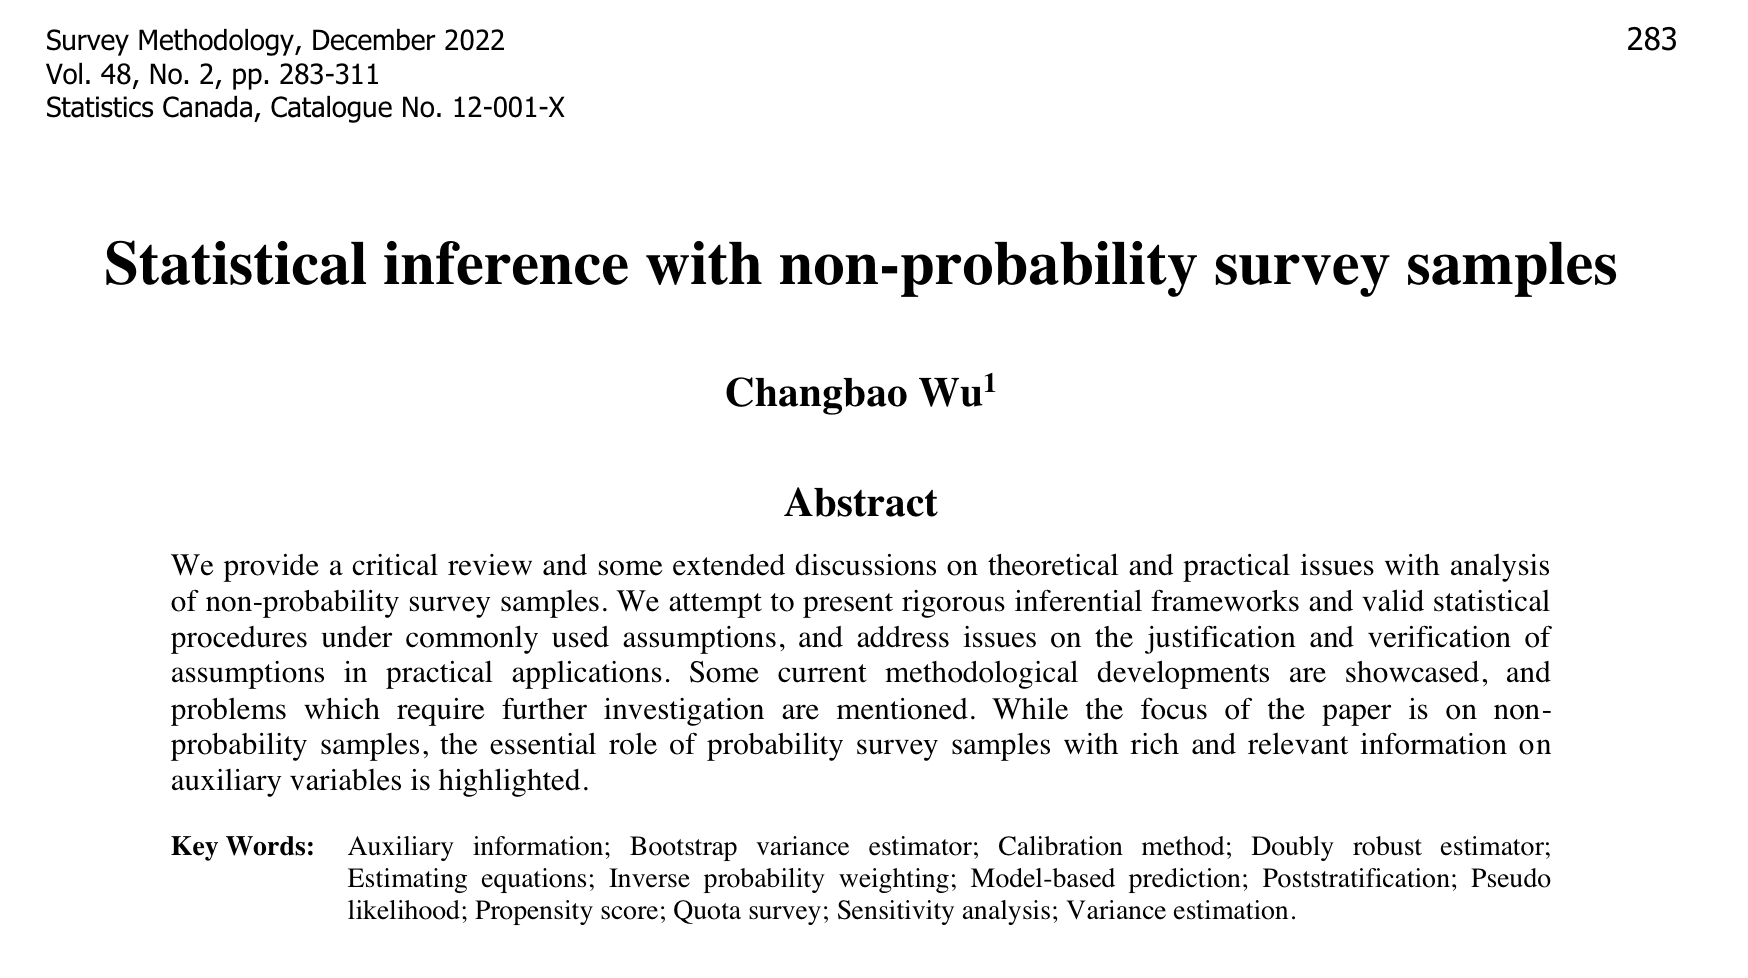
\includegraphics[width=\textwidth]{fig-4-meth/ps-review.png}
\end{center}
\end{frame}

\begin{frame}{Nazewnictwo}
    \begin{itemize}
    \justifying
        \item Propensity score (PS) -- prawdopodobieństwa inkluzji do próby nielosowej $S_A$
        \item Propensity score weighting (PSW) / Inverse probability weighting (IPW) -- ważenie przez odwrotność prawdopodobieństwa inkluzji 
    \end{itemize}
\end{frame}

\begin{frame}{Wprowadzenie do metody IPW}
    \begin{itemize}
    \justifying
        \item Inverse Probability Weighting (IPW) to popularna metoda estymacji wykorzystująca prawdopodobieństwa włączenia do próby
        \item Opiera się na estymacji prawdopodobieństwa włączenia (PS) danego wzorem $\pi_i^A=P\left(i \in S_A \right)$
        \item Metoda szczególnie przydatna w kontekście próby nielosowej
        \item Prawdopodobieństwa włączenia są używane do korygowania obciążeń wynikających z mechanizmu selekcji próby
    \end{itemize}
\end{frame}

\begin{frame}{Dwa warianty estymatora IPW}
    Metoda IPW oferuje dwa główne warianty estymatora średniej populacyjnej:
    
    \begin{equation}
      \hat{\mu}_{y,\text{IPW1}}=\frac{1}{N} \sum_{i \in S_A} \frac{y_i}{\hat{\pi}_i^A} \quad \text { i } \quad 
      \hat{\mu}_{y,\text{IPW2}}=\frac{1}{\hat{N}^A} \sum_{i \in S_A} \frac{y_i}{\hat{\pi}_i^A},
    \end{equation}
    
    gdzie:
    \begin{itemize}
        \item $\hat{\mu}_{y,\text{IPW1}}$ - modyfikacja estymatora Horvitza-Thompsona
        \item $\hat{\mu}_{y,\text{IPW2}}$ - modyfikacja estymatora Hájeka
        \item $\hat{N}^A = \sum_{i \in S_A} (\pi_i^A)^{-1}$ - oszacowana liczebność populacji
    \end{itemize}
    
    \vspace{0.5em}
    \small{Wu (2022) zauważa, że estymator $\hat{\mu}_{y,\text{IPW2}}$ daje lepsze wyniki niż $\hat{\mu}_{y,\text{IPW1}}$ nawet gdy liczebność populacji jest znana.}
\end{frame}

\begin{frame}{Konstrukcja estymatora IPW}
    Budowa estymatora IPW wymaga dwóch kroków:
    
    \begin{enumerate}
        \item Estymacja prawdopodobieństw włączenia $\pi_i^A$
        \item Wyznaczenie wag $d_i^A = 1/\pi_i^A$
    \end{enumerate}
    
    \vspace{1em}
    
    Do estymacji prawdopodobieństw $\pi_i^A=\pi(\bx_i, \bgamma)$ można zastosować metodę największej wiarygodności, zakładając, że informacje o $\bx_i$ są dostępne dla każdej jednostki w populacji (lub próby losowej).
\end{frame}

\begin{frame}{Regresja logistyczna w estymacji PS}
    \begin{itemize}
    \justifying
        \item W praktyce, do modelowania prawdopodobieństwa włączenia $\pi(\bx_i, \bgamma)$ najczęściej stosuje się regresję logistyczną
        \item Model logistyczny przyjmuje postać:
        
        \begin{equation}
        \pi(\bx_i, \bgamma) = \frac{\exp(\bx_i^T \bgamma)}{1 + \exp(\bx_i^T \bgamma)}
        \end{equation}
        
        \item Parametry $\bgamma$ mają interpretację logarytmu ilorazu szans
        \item Model jest elastyczny i może uwzględniać zmienne ilościowe, jakościowe oraz interakcje
    \end{itemize}
\end{frame}

\begin{frame}{Estymacja modelu logistycznego}
    \begin{itemize}
    \justifying
        \item Do estymacji parametrów $\bgamma$ modelu logistycznego używamy próby nielosowej ($S_A$) i losowej ($S_B$)
        \item Jednostki z próby nielosowej traktujemy jako "sukcesy"\; ($R_i^A = 1$)
        \item Jednostki z próby losowej traktujemy jako "porażki"\; ($R_i^A = 0$)
        \item Zmienne objaśniające $\bx_i$ powinny dobrze przewidywać mechanizm włączenia do próby nielosowej
        \item Ważne jest uwzględnienie wag $d_i^B$ z próby losowej w procesie estymacji
    \end{itemize}
    
    \vspace{0.5em}
    
    \alert{Uwaga:} Jakość oszacowań $\hat{\pi}_i^A$ bezpośrednio wpływa na jakość finalnego estymatora IPW. Istotny jest dobór odpowiednich zmiennych pomocniczych $\bx_i$ silnie związanych zarówno z mechanizmem włączenia do próby jak i zmienną badaną $y$.
\end{frame}

\begin{frame}{Warunki stosowania modelu logistycznego}
    \begin{itemize}
    \justifying
        \item Wymaga spełnienia założenia MAR (Missing At Random) - prawdopodobieństwo włączenia do próby zależy tylko od obserwowalnych zmiennych $\bx_i$
        \item Wymaga odpowiedniego pokrycia przestrzeni zmiennych pomocniczych w próbie losowej i nielosowej
        \item Możliwe jest rozszerzenie do bardziej złożonych modeli (np. modele GAM, lasy losowe) jeśli relacja nie jest liniowa w logicie
    \end{itemize}
    
    \vspace{1em}
    
    Po estymacji modelu, otrzymane prawdopodobieństwa $\hat{\pi}_i^A$ są używane do konstruowania wag $\hat{d}_i^A = 1/\hat{\pi}_i^A$ stosowanych w estymatorach IPW.
\end{frame}

\begin{frame}{Funkcja wiarygodności}
    Teoretyczna funkcja logarytmu wiarygodności ma postać:
    
    \begin{align}
    \small
    \ell(\bgamma) &= \log\left\{\prod_{i=1}^N \left(\pi_i^A\right)^{R_i}\left(1-\pi_i^A\right)^{1-R_i}\right\} \nonumber \\
    &= \sum_{i \in S_{A}} \log \left\{\frac{\pi\left(\bx_i, \bgamma\right)}{1-\pi\left(\bx_i, \bgamma\right)}\right\}+\sum_{i=1}^N \log \left\{1-\pi\left(\bx_i, \bgamma\right)\right\}.
    \end{align}
    
    \vspace{0.5em}
    
    W praktyce funkcja tej postaci nie może być stosowana, ponieważ nie wszystkie jednostki z populacji są obserwowane.
\end{frame}

\begin{frame}{Pseudo funkcja wiarygodności}
    Bardziej realistyczne podejście polega na wykorzystaniu referencyjnej próby losowej $S_B$. Wtedy otrzymujemy pseudo funkcję logarytmu wiarygodności:
    
    \begin{equation}
    \small
    \ell^*(\bgamma) = \sum_{i \in S_{A}} \log \left\{\frac{\pi\left(\bx_i, \bgamma\right)}{1-\pi\left(\bx_i, \bgamma\right)}\right\} + \sum_{i \in S_{B}} d_i^B \log \left\{1-\pi\left(\bx_i, \bgamma\right)\right\}.
    \end{equation}
    
    \vspace{0.5em}
    
    Estymator $\hat{\bgamma}$ największej pseudo-wiarygodności można uzyskać jako rozwiązanie równania pseudo-score, które przy założeniu funkcji logitowej dla $\pi_i^A$ ma postać:
    
    \begin{equation}
    \small
    \bU(\bgamma) = \sum_{i \in S_A} \bx_i - \sum_{i \in S_B} d_i^B \pi(\bx_i, \bgamma) \bx_i.
    \end{equation}
\end{frame}

\begin{frame}{}
    Przejdźmy do przykładu w R
\end{frame}

\begin{frame}{Ograniczenia IPW MLE}
Estymacja $\pi(\bx_i, \bgamma)$ z wykorzystaniem metody MLE lub pseudo-MLE ma następujące ograniczenia
    \begin{itemize}
        \item  działa tylko jeżeli model dla $\pi(\bx_i, \bgamma)$ jest poprawnie wyspecifykowany,
        \item może skutkować dużymi wagami gdy $\pi(\bx_i, \bgamma)$ jest małe,
        \item wariancja wag zwykle jest większa,
        \item wagi $1/\pi(\bx_i, \bgamma)$ nie odtwarzają wartości globalnych z próby lub populacji,
        \item możemy zastosować tylko gdy dysponujemy danymi z populacji lub próby.
    \end{itemize}
\end{frame}


\begin{frame}{Rozszerzenia i metoda kalibracji}
    Funkcja $\bU(\bgamma)$ może być zastąpiona przez ogólne równania estymujące (ang. \textit{generalized estimation equations}; GEE). 
    
    \begin{itemize}
        \item Niech $\bh(\bx, \bgamma)$ będzie wektorem funkcji o tym samym wymiarze co $\bgamma$
        \item Definiujemy funkcję $\bG(\bgamma)$ jako:
        
        \begin{equation}
        \bG(\bgamma)=\sum_{i \in S_A} \bh\left(\bx_i, \bgamma\right)-\sum_{i \in S_B} d_i^B \pi\left(\bx_i, \bgamma\right) \bh\left(\bx_i, \bgamma\right)
        \end{equation}
        
        \item Rozwiązanie równania $\bG(\bgamma)=\bZero$ daje zgodny estymator $\hat{\bgamma}$
        \item Najczęściej wybierane funkcje to 
        \begin{itemize}
            \item $\bh\left(\bx_i, \bgamma\right) = \bx_i \pi\left(\bx_i, \bgamma\right)^{-1}$,
            \item $\bh\left(\bx_i, \bgamma\right) = \bx_i$ (prowadzi do $\bU(\bgamma)$).
        \end{itemize} 
    \end{itemize}
    
    Dla drugiego wariantu funkcji $\bh$ otrzymujemy \textit{skalibrowane} IPW:
    
    \begin{equation}
    \bG(\btheta) = \sum_{i \in S_A} \frac{\bx_i}{\pi\left(\bx_i, \bgamma\right) }-\sum_{i \in S_B} d_i^B \bx_i.
    \label{eq-ipw-gee}
    \end{equation}
    
\end{frame}

\begin{frame}{Rozszerzenia i metoda kalibracji}
Proszę zauważyć, że dla \eqref{eq-ipw-gee} sumę daną wzorem $\sum_{i \in S_B} d_i^B \bx_i$ możemy zastąpić wartościami globalnym (znanymi z populacji)

    \begin{equation}
    \bG(\btheta) = \sum_{i \in S_A} \frac{\bx_i}{\pi\left(\bx_i, \bgamma\right)} -\btau_{\bx} = 
    \begin{bmatrix}
    \sum_{i \in S_A} \frac{\bx_{i1}}{\pi\left(\bx_i, \bgamma\right)} \\
    \sum_{i \in S_A} \frac{\bx_{i2}}{\pi\left(\bx_i, \bgamma\right)} \\
    ... \\
    \sum_{i \in S_A} \frac{\bx_{ip}}{\pi\left(\bx_i, \bgamma\right)} 
    \end{bmatrix} - 
    \begin{bmatrix}
     \tau_{x_1} \\
     \tau_{x_2} \\
     ... \\
     \tau_{x_p}
    \end{bmatrix}
    \end{equation}
    
Kim i Riddles (2012) pokazali, że gdy estymujemy $\bgamma$ z wykorzystaniem GEE to estymator IPW jest podwójnie odporny przy założeniu, że model zmiennej wynikowej (Y) jest liniowy (tj. liniowy w populacji).
 
\end{frame}


\begin{frame}{Rozszerzenia i metoda kalibracji}
Metoda GEE ma następujące własności:
    \begin{itemize}
    \justifying
        \item estymator ten jest podwójnie odporny i.e. kalibrując do znanych wartości globalnych zakładamy, że model $E(Y|X)$ jest liniowy, por. Kim  and Riddles (2012). \textit{Some theory for propensity scoring adjustment estimator}, Survey Methodology 38, 157-165 -- oznacza to, że jeżeli model dla $\pi\left(\bx_i, \bgamma\right)$ będzie źle wyspecifykowany ale model $E(Y|X)$ jest liniowy to estymator dostarczy nam (asymptotycznie) nieobciążonych szacunków.
        \item wagi $1/\pi\left(\bx_i, \bgamma\right)$ odtwarzają wartości globalne,
        \item estymator GEE możemy stosować gdy nie mamy dostępu do danych jednostkowych a jedynie wartości globalnych,
        \item wariancja estymatora GEE jest zwykle mniejsza niż IPW,
        \item wariancja wag $1/\pi\left(\bx_i, \bgamma\right)$ w przypadku metody GEE jest zwykle mniejsza i zwykle unikamy wag ekstremalnych.
    \end{itemize}
\end{frame}

\begin{frame}{Estymacja wariancji IPW}
\begin{itemize}
\justifying
    \item Chen et al. (2020) przedstawili postać analityczną oraz metodę bootstrap umożliwiającą estymację wariancji estymatora IPW dla średniej.
    \item W pakiecie \texttt{nonprobsvy} zaimplementowaliśmy zarówno podejście analityczne, jak i metodę bootstrap.
    \item Idea metody bootstrap polega na, $b=1,...,B$ razy powtarzamy
    \begin{enumerate}
        \item Losujemy ze zwracaniem jednostki z próby $S_A$ (nielosowej)
        \item Losujemy ze zwracaniem jednostki z próby $S_B$ (losowej) zgodnie ze schematem losowania.
        \item Estymujemy parametry $\bgamma$ funkcji propensity score $\pi\left(\bx_i, \bgamma\right)$ i wyznaczamy $\hat{\mu}_{y,\text{IPW2},b}$
    \end{enumerate}
    Następnie wyznaczamy wariancję z wektora oszacowań 
    
    $$
    \left(\hat{\mu}_{y,\text{IPW2},1}, \hat{\mu}_{y,\text{IPW2},2}, ..., \hat{\mu}_{y,\text{IPW2},b}\right)^T.
    $$
\end{itemize}
\end{frame}

\begin{frame}{}
    Przejdźmy do przykładu w R
\end{frame}

\subsection{Podejście predykcyjne}

\begin{frame}{Model semi-parametryczny w podejściu predykcyjnym}
\begin{itemize}
    \item W podejściu predykcyjnym zakłada się semi-parametryczny model dla populacji skończonej:
    \begin{equation*}
    E_{\xi}\left(y_i \mid \bx_i\right)=m\left(\bx_i, \bbeta\right), \quad V_{\xi}\left(y_i \mid \bx_i\right)=v\left(\bx_i\right) \sigma^2.
    \end{equation*}
    \item Funkcje $m(\cdot,\cdot)$ i $v(\cdot)$ mają znane formy.
    \item $y_i$ są warunkowo niezależne, gdy dane są $\bx_i$.
    \item Model obowiązuje dla wszystkich jednostek populacji $U$ (model super-populacyjny) -- parametry $\bbeta$ szacujemy na próbie nieprobabilistycznej $S_A$ i przenosimy na pozostałe jednostki populacji.
    \item Parametry modelu można oszacować metodą quasi-największej wiarygodności.
\end{itemize}
\end{frame}

\begin{frame}{Pytania badawcze}
    \begin{itemize}
        \item a co jeśli $m(\cdot,\cdot)$  i $v(\cdot)$ źle wyspecyfikujemy?
        \item a co jeśli $y_i$ są warunkowo \textbf{zależne}, gdy dane są $\bx_i$?
        \item a co jeśli nie możemy przenieść $\bbeta$? kiedy?
    \end{itemize}
\end{frame}





\begin{frame}{Estymatory predykcyjne}
\begin{itemize}
    \item Dwa powszechnie stosowane estymatory predykcyjne:
    \begin{equation*}
    \hat{\mu}_{y,\text{PR1}}=\frac{1}{N} \sum_{i=1}^N \hat{m}_i \quad \text{i} \quad \hat{\mu}_{y,\text{PR2}}=\frac{1}{N}\left\{\sum_{i \in S_A} y_i-\sum_{i \in S_A} \hat{m}_i+\sum_{i=1}^N \hat{m}_i\right\}.
    \end{equation*}
    \item Dla modeli liniowych, gdzie $m(\bx_i, \bbeta)=\bx_i^{\prime}\bbeta$, estymatory upraszczają się do:
    \begin{equation*}
    \hat{\mu}_{y,\text{PR1}}=\mu_{\bx}^{\prime} \hat{\bbeta} \quad \text{i} \quad \hat{\mu}_{y,\text{PR2}}=\frac{n_A}{N}\left(\bar{y}_A-\overline{\bx}_A^{\prime} \hat{\bbeta}\right)+\mu_{\bx}^{\prime} \hat{\bbeta}.
    \end{equation*}
    \item Jeśli model liniowy zawiera wyraz wolny i $\hat{\bbeta}$ jest estymatorem najmniejszych kwadratów, to $\hat{\mu}_{y,\text{PR1}}=\hat{\mu}_{y,\text{PR2}}$.
\end{itemize}
\end{frame}

\begin{frame}{Korzyści z estymatorów predykcyjnych}
\begin{itemize}
    \item Formuła $\hat{\mu}_{y,\text{PR2}}$ wymaga tylko:
    \begin{itemize}
        \item próby nieprobabilistycznej $S_A$,
        \item średnich populacyjnych (lub sum i wielkości populacji $N$).
    \end{itemize}
    \item Jeśli średnie populacyjne są nieznane, można je zastąpić estymatorami z referencyjnej próby probabilistycznej $S_B$ (model $\hat{m}_i$ jest dopasowany na $S_A$ i stosowany na $S_B$):
    \begin{itemize}
        \item $\sum_{i=1}^N \hat{m}_i$ zastępuje się przez $\sum_{i \in S_B} d_i^B\hat{m}_i$
        \item $\mu_{\bx}$ zastępuje się przez $\hat{\mu}_{\bx}=(\hat{N}^B)^{-1}\sum_{i \in S_B}d_i^B\bx_i$, gdzie $\hat{N}^B=\sum_{i \in S_B}d_i^B$.
    \end{itemize}
\end{itemize}
\end{frame}

\begin{frame}{Podejście oparte na modelu}
    \begin{figure}
        \centering
        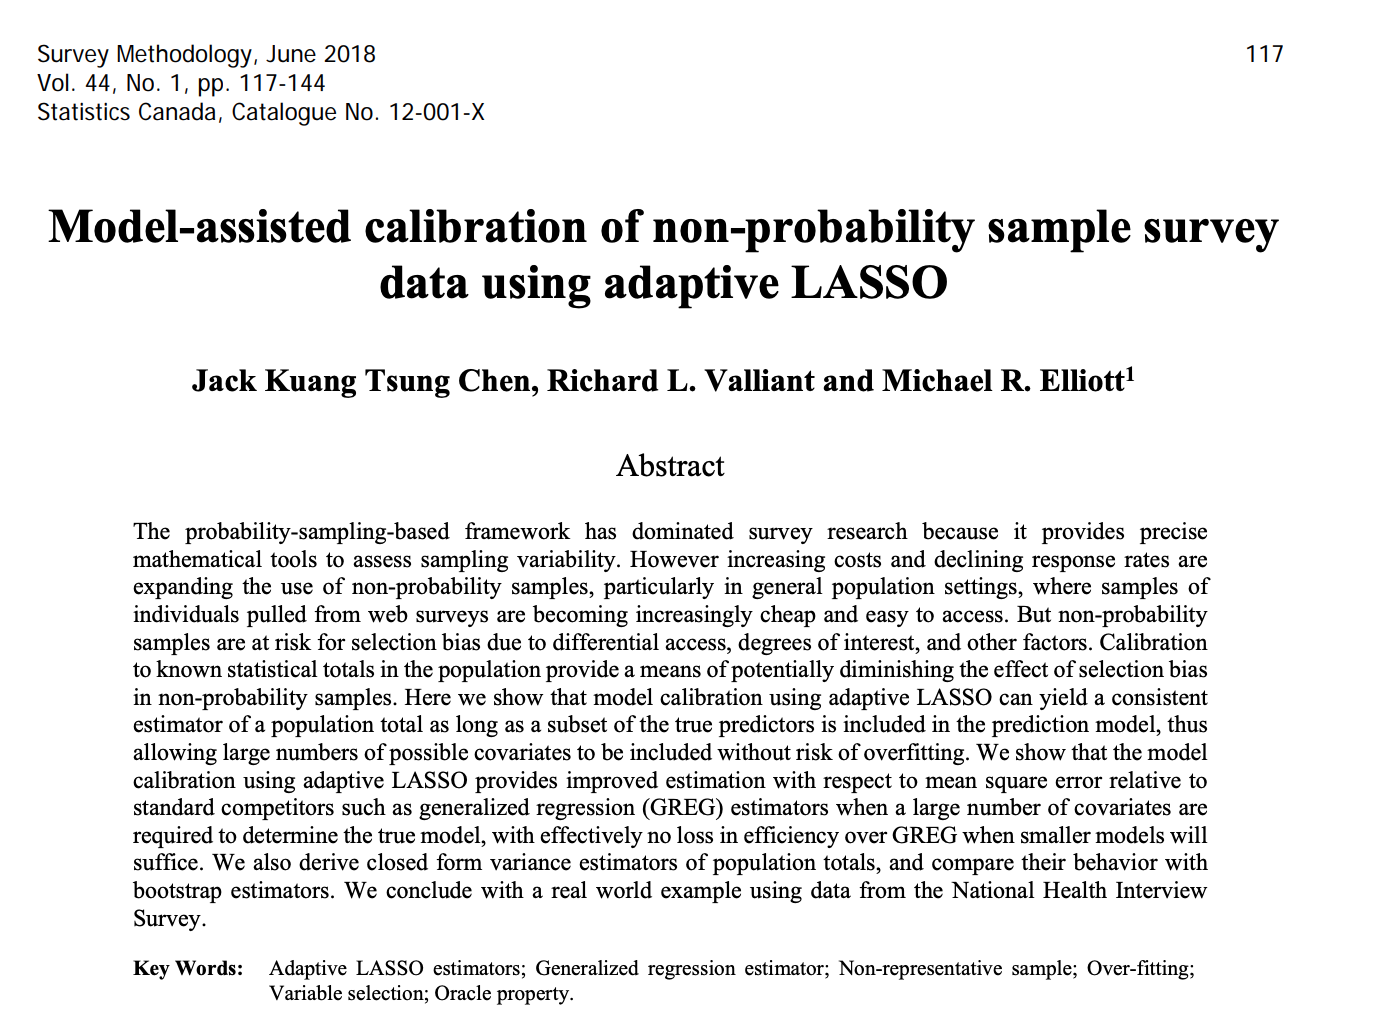
\includegraphics[width=0.8\textwidth]{fig-6-model/model-1.png}
    \end{figure}
\end{frame}

\begin{frame}{Podejście oparte na modelu}
    \begin{figure}
        \centering
        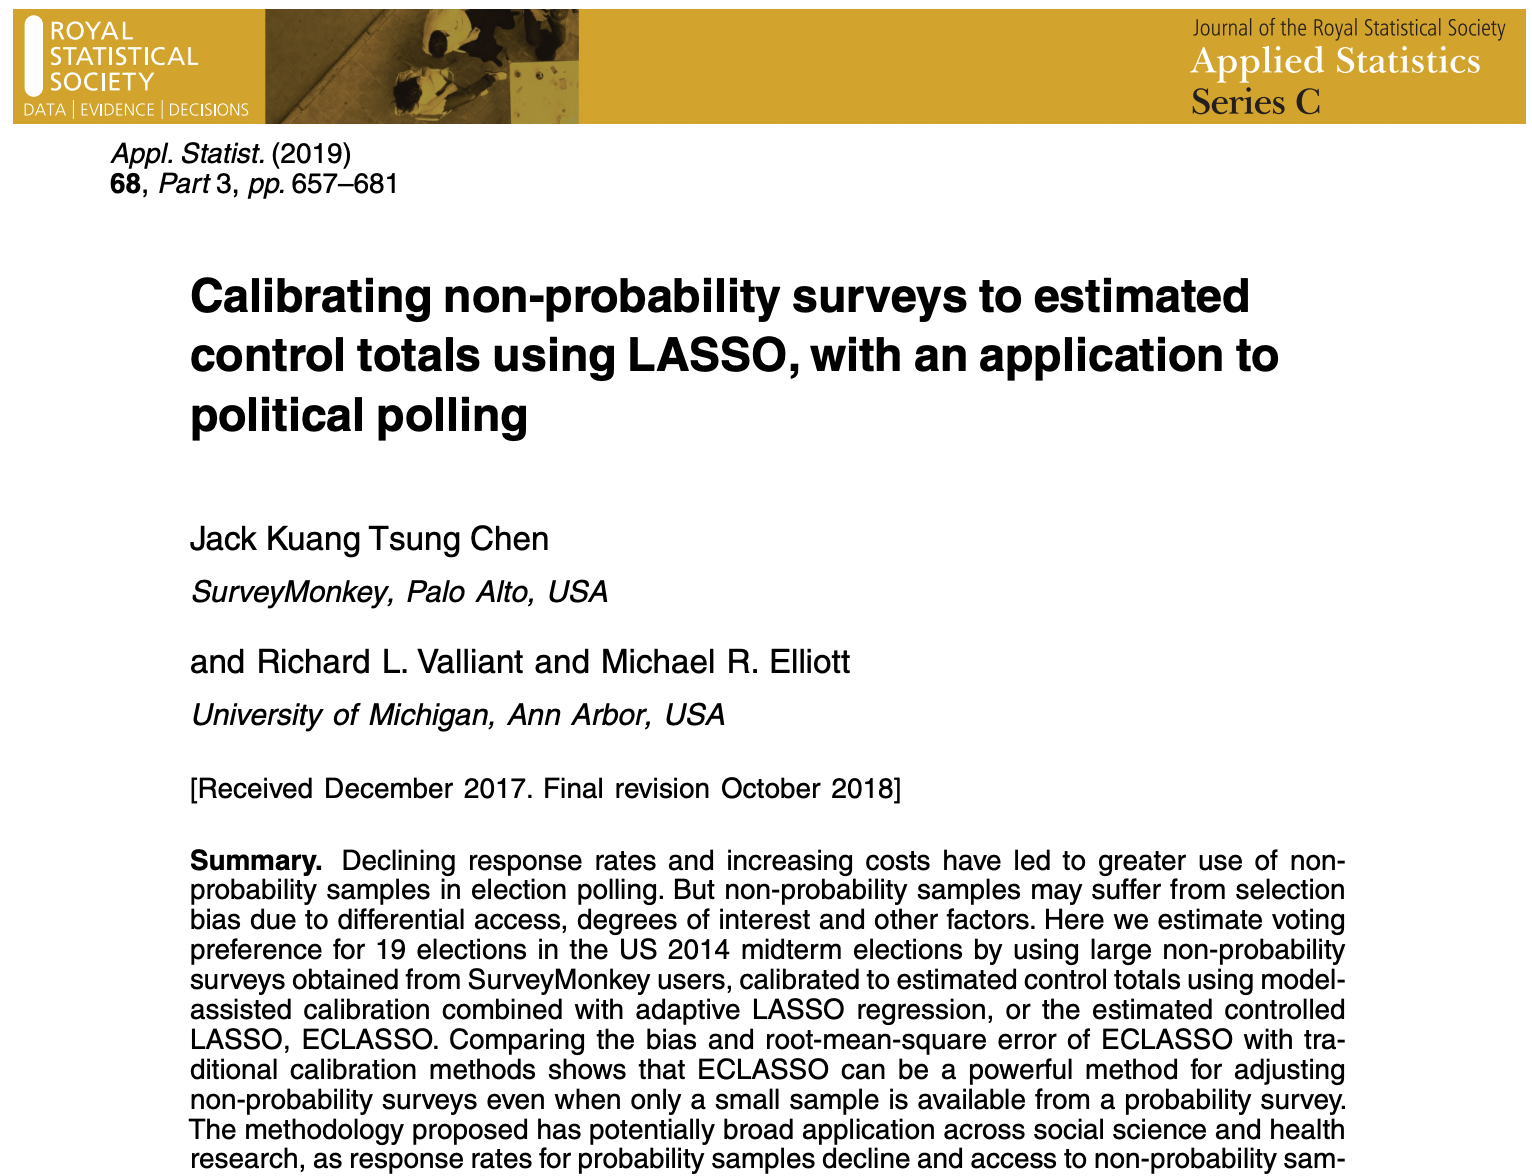
\includegraphics[width=0.8\textwidth]{fig-6-model/model-2.png}
    \end{figure}
\end{frame}

\begin{frame}{Podejście oparte na modelu}
    \begin{figure}
        \centering
        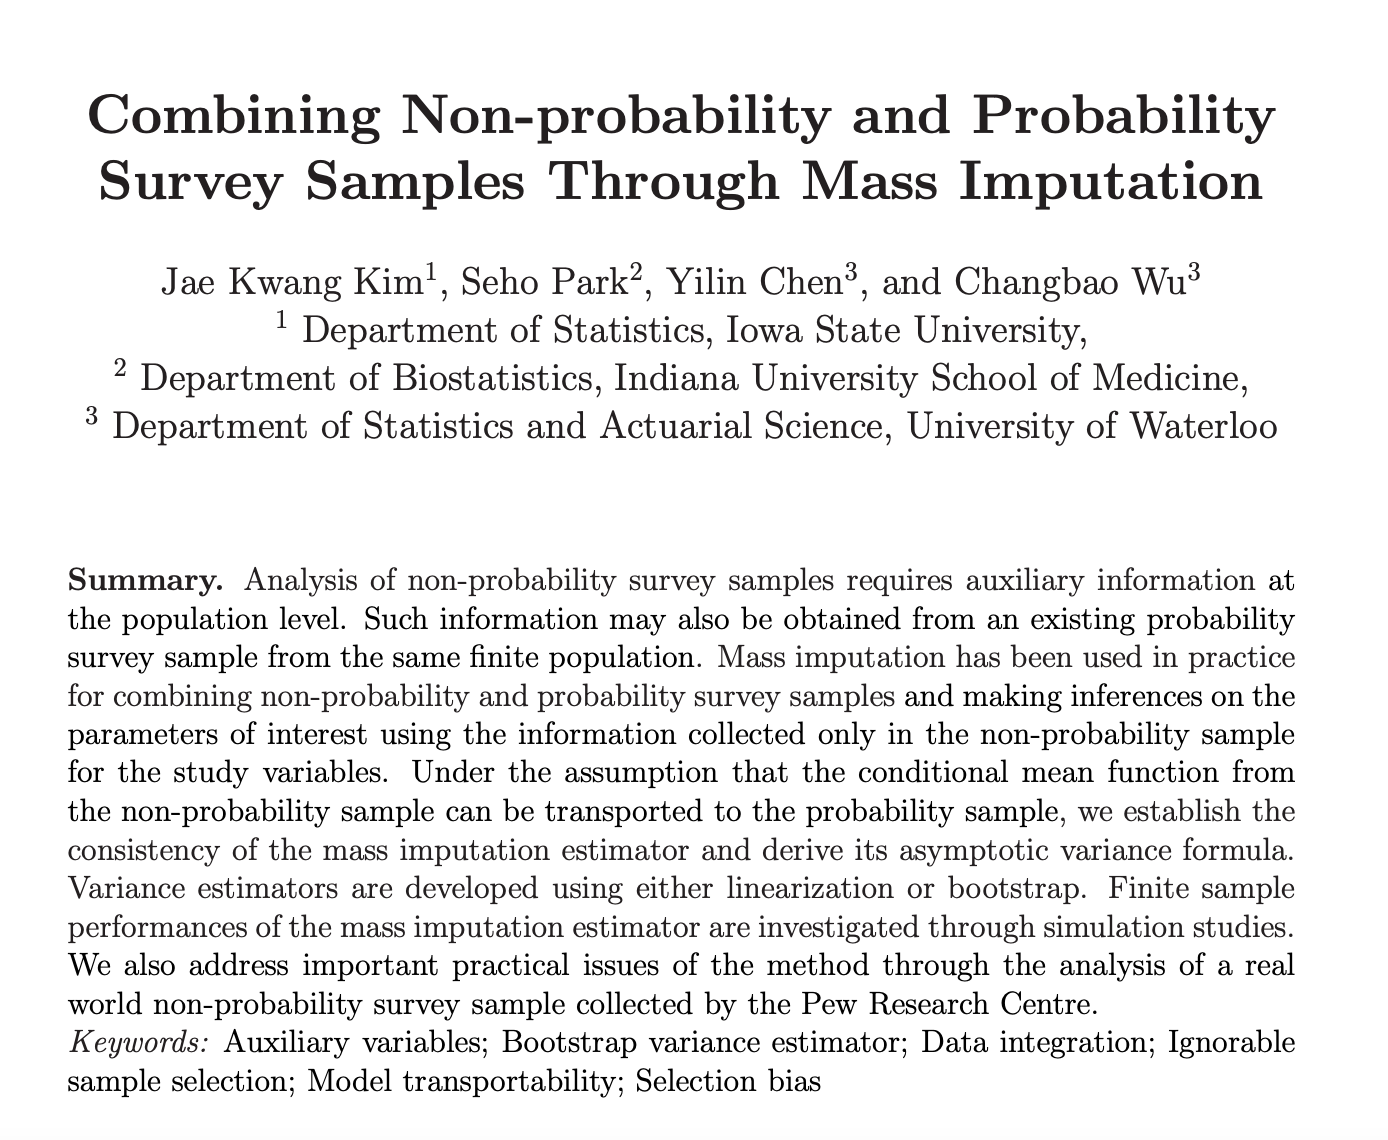
\includegraphics[width=0.8\textwidth]{fig-6-model/model-3.png}
    \end{figure}
\end{frame}



\begin{frame}{Podejście oparte na modelu -- klasyfikacja metod}
\begin{itemize}
    \item Gdy znamy wszystkie jednostki z populacji,
    \item Gdy znamy tylko jednostki z próby nielosowej -- masowa imputacja (metoda Riversa, metody opracowane przez Jae-Kwang Kim'a i współpracowników).
\end{itemize}
\end{frame}

\begin{frame}{Podejście oparte na modelu -- założenia}
    \begin{itemize}
        \item Model z próby losowej możemy przenieść na resztę jednostek (ang. missing at random) -- tzw. model dla super-populacji.
        \item Dysponujemy zmiennymi $\boldsymbol{X}$, które są obserwowane w próbie/próbach i~populacji.
        \item Możemy zidentyfikować jednostki między próbą nielosową i populacją.
        \item Zakładamy, że zmienna $Y$ oraz  $\boldsymbol{X}$ są obserwowane bez błędów.
        \item Zakładamy brak korelacji między obserwacjami, brak błędu nadreprezentacji itp. 
    \end{itemize}
\end{frame}


\begin{frame}{Masowa imputacja -- dwa podejścia}
\begin{figure}
    \centering
    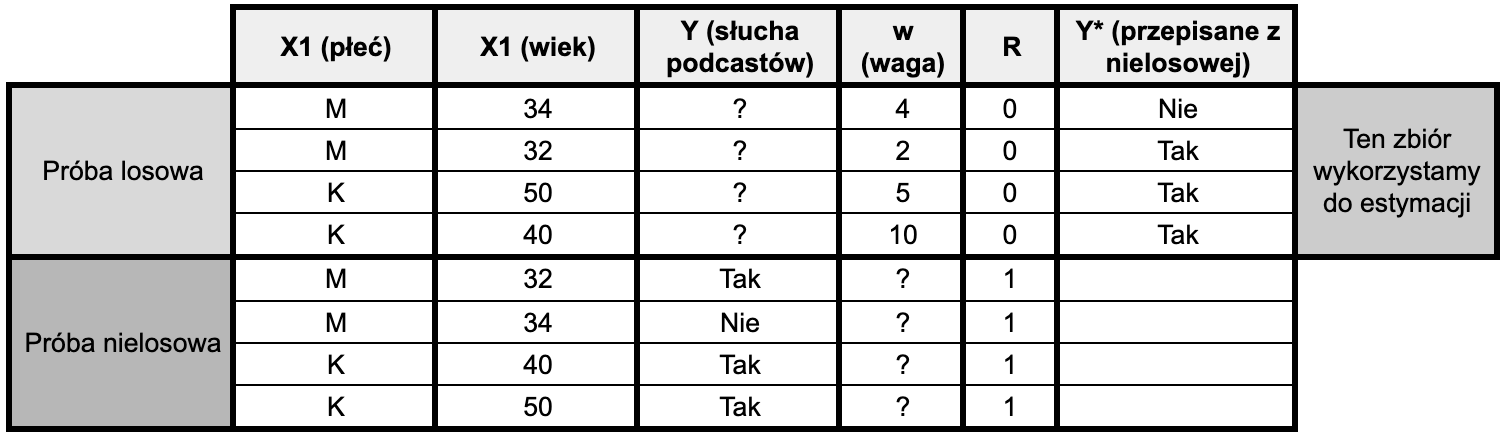
\includegraphics[width=0.7\textwidth]{fig-6-model/mass-1.png}
    \caption{Podejście I: Przepisanie wartości z próby nielosowej}
\end{figure}
\begin{figure}
    \centering
    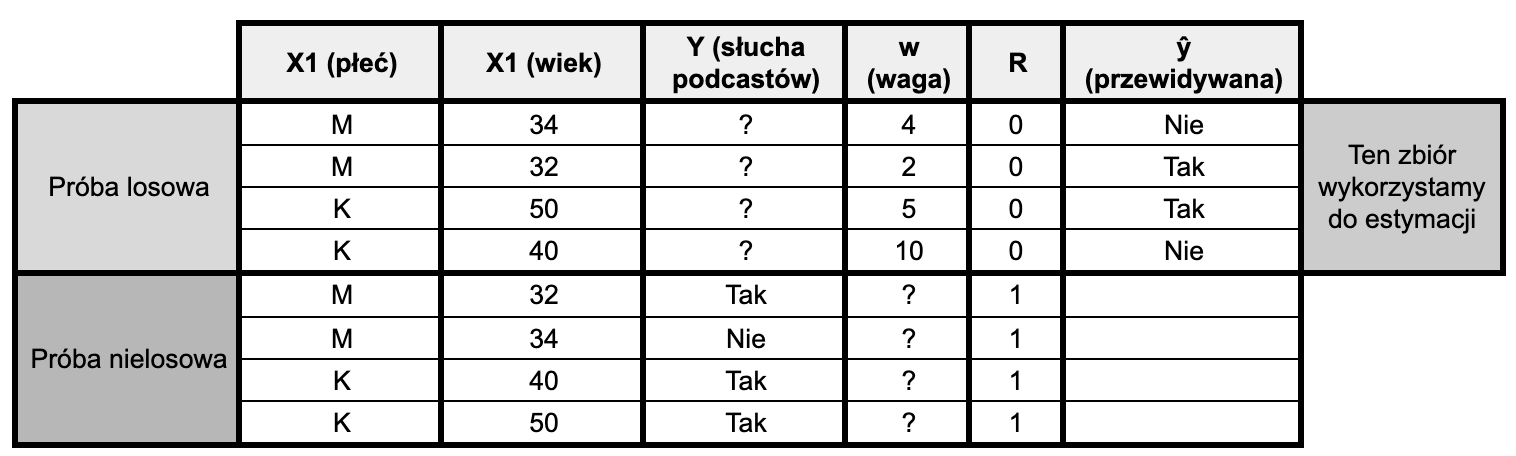
\includegraphics[width=0.7\textwidth]{fig-6-model/mass-2.png}
    \caption{Podejście II: wartości przewidywane z modelu zbudowanego na próbie nielosowej}
\end{figure}
\end{frame}


\begin{frame}{Masowa imputacja -- podejście I}
W pierwszym podejściu, zaproponowanym przez Rivers (2007), dokonujemy masowej imputacji przez tzw. sample matching, który polega na następujących krokach:
\begin{enumerate}
    \item Dla próby nielosowej $S_A$ oraz losowej $S_B$ określamy zestaw wspólnych cech $\bx$.
    \item Następie, dla każdej jednostki $i \in S_B$ szukamy najbliższej jednostki ze zbioru $k \in S_A$, tak żeby
    \begin{equation}
        d(\bx_k, \bx_i) =  || \bx_k - \bx_i||
    \end{equation}
    była jak najmniejsza. Możemy w tym celu wykorzystać np. odległość euklidesową. Jednostce $i$ przypisujemy wartość cechy $y_k$ ze zbioru $S_A$.
    \item Po znalezieniu odpowiednich sąsiadów, wyznaczamy estymator. Przykładowo, estymator wartości średniej dany będzie:
    \begin{equation}
        \hat{\mu}_{y,\text{MI-NN}} = \sum_{i \in S_B} d_i^B y_i / \sum_{i \in S_B} d_i^B.
    \end{equation}
\end{enumerate}
\end{frame}

\begin{frame}{Masowa imputacja -- podejście I -- UWAGA}
Na podstawie pracy: Abadie \& Imbens (2006) \textbf{Large sample properties of matching estimators for average treatment effects} (Econometrica, 74(1), 235-267) można wykazać, że obciążenie estymatora $\hat{\mu}_{y,\text{MI-NN}}$ rośnie wraz z liczbą zmiennych użytych do obliczenia $d(\bx_k, \bx_i)$. Dokładnie:

\begin{equation}
    \text{Bias}(\hat{\mu}_{y,\text{MI-NN}}) = O_p\left(n_A^{-1/p}\right)
\end{equation}

gdzie $p$ to wymiar wektora $\bx_k$ (liczba ciągłych zmiennych pomocniczych), a $n_A$ to liczebność próby \textbf{nielosowej} $S_A$ (puli, z której losujemy sąsiadów).

\vspace{0.3cm}

Oznacza to, że estymator $\hat{\mu}_{y,\text{MI-NN}}$ jest $\sqrt{n}$-zgodny wyłącznie gdy $p=1$ (obciążenie $O_p(n_A^{-1})$); dla $p \geq 2$ obciążenie jest tego samego rzędu lub większe od błędu standardowego.

\vspace{0.2cm}
\small{Wynik dotyczy zmiennych ciągłych. W przypadku zmiennych kategorycznych możliwy jest \textit{exact matching} -- obciążenie zależy wtedy od liczebności komórek.}
\end{frame}

\begin{frame}{Asymptotyczne obciążenie przy stałej liczbie sąsiadów}
    \begin{figure}
        \centering
        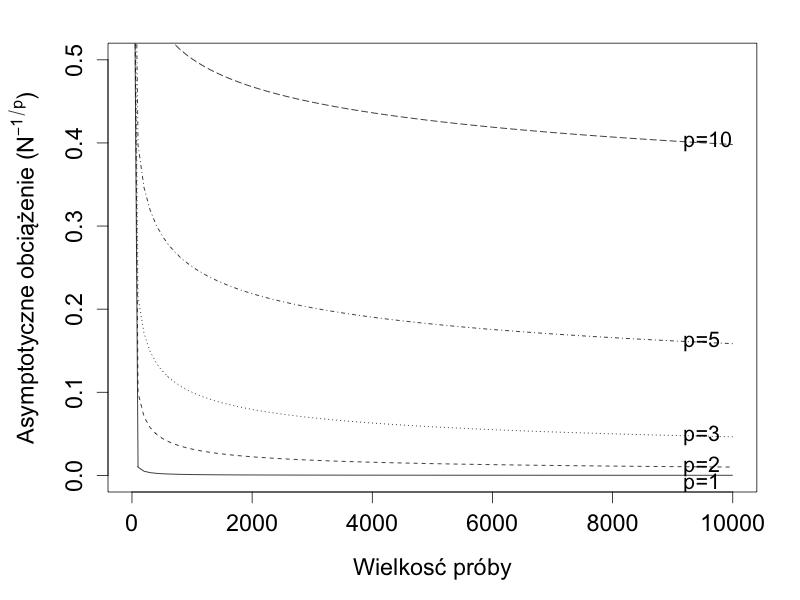
\includegraphics[width=0.6\textwidth]{figs/assymp-bias.png}
        \caption{Wizualizacja asymptotycznego obciążenia estymatora MI NN }
    \end{figure}
\end{frame}

\begin{frame}{Masowa imputacja -- podejście I -- Praktyka}

Mając na uwadze fakt, że przypisania wartości $y_i$ z próby nielosowej dla jednostek $k$ z próby losowej należy wykorzystać na podstawie wyłącznie jednej zmiennej, stosuje się następujące podejście:

\begin{enumerate}
    \item Budujemy model $m(\bx_i; \bbeta)$ na próbie nielosowej $S_A$ otrzymując $\hat{y}_i = m(\bx_i; \hat{\bbeta})$.
    \item Stosujemy model $m(\bx; \hat{\bbeta})$ na próbie losowej $S_B$ otrzymując $\hat{y}_k = m(\bx_k; \hat{\bbeta})$.
    \item Dla każdej jednostki $k \in S_B$ znajdujemy najbliższą jednostkę na podstawie $d(\hat{y}_k, \hat{y}_{i})$ i przepisujemy wartość $y_i$.
    \item Następnie wyznaczamy estymator

        \begin{equation}
        \hat{\mu}_{y,\text{MI-PMM}} = \sum_{i \in S_B} d_i^B y_i / \sum_{i \in S_B} d_i^B.
    \end{equation}

\end{enumerate}
To podejście w literaturze nazywa się \textit{predictive mean matching}.
\end{frame}

\begin{frame}{Masowa imputacja -- podejście II}

\begin{itemize}
    \item W pracy Kim,  Park, Chen i Wu (2021) \textbf{Combining Non-probability and Probability Survey Samples Through Mass Imputation}, (Journal of the Royal Statistical Society: Series A) zaproponowano trochę inne podejście ale oparte na solidnych, teoretycznych podstawach.
    \item Zamiast dokonywać poszukiwania najbliższego sąsiada wykorzystuje się wyłącznie 1 oraz 2 krok z poprzedniego slajdu.
    \item Estymator wartości średniej dany jest wtedy
         \begin{equation}
        \hat{\mu}_{y,\text{MI-K}} = \sum_{i \in S_B} d_i^B\hat{y}_i / \sum_{i \in S_B} d_i^B.
    \end{equation}
    \item Ten sposób nazywamy na potrzeby zajęć podejściem II do masowej imputacji.
    \item W wyżej wymienionej pracy zaproponowano również estymator wariancji w postaci zlinearyzowanej (konkretny wzór), jak i na podstawie metody bootstrap.
\end{itemize}
\end{frame}

\begin{frame}{Masowa imputacja -- przykład empiryczny}
\begin{center}
Przejdźmy do przykładu    
\end{center}
\end{frame}

\end{document}


